
%% Run LaTeX on this file several times to get Table of Contents,
\input{book_command}
%\includeonly{week3/Tuesday}
\includeonly{week5/Friday}
\begin{document}
%Hello
\frontmatter
%%%%%%%%%%%%%%%%%%%%%%%%%%%%%%%%%%%%%%%%%%%%%%%%%%%%%%%%%%%%%%%%
%%%Command
%% Title Pages
%% Wiley will provide title and copyright page, but you can make
%% your own titlepages if you'd like anyway
%% Setting up title pages, type in the appropriate names here:

\booktitle{A First Course \\ In \\
Linear Algebra}

\subtitle{MAT2040 Notebook}

\AuAff{Prof. Tom Luo\\ The Chinese University of Hongkong, Shenzhen}
\AuAff{Prof. Ruoyu Sun\\ University of Illinois Urbana-Champaign}
%\AuAff{Michael D. Logothetis\\ University of Patras}

%% \\ will start a new line.
%% You may add \affil{} for affiliation, ie,
%\authors{Robert M. Groves\\
%\affil{Universitat de les Illes Balears}
%Floyd J. Fowler, Jr.\\
%\affil{University of New Mexico}
%}

%% Print Half Title and Title Page:
\halftitlepage
\titlepage

%%%%%%%%%%%%%%%%%%%%%%%%%%%%%%%%%%%%%%%%%%%%%%%%%%%%%%%%%%%%%%%%
%% Copyright Page

%\begin{copyrightpage}{year}
%Title, etc
%\end{copyrightpage}

% Note, you must use \ to start indented lines, ie,
% 
 \begin{copyrightpage}{2004}
 Survey Methodology / Robert M. Groves . . . [et al.].
 \       p. cm.---(Wiley series in survey methodology)
 \    ``Wiley-Interscience."
 \    Includes bibliographical references and index.
 \    ISBN 0-471-48348-6 (pbk.)
 \    1. Surveys---Methodology.  2. Social 
 \  sciences---Research---Statistical methods.  I. Groves, Robert M.  II. %
 Series.\\

 HA31.2.S873 2004
 001.4'33---dc22                                             2004044064
 \end{copyrightpage}

%%%%%%%%%%%%%%%%%%%%%%%%%%%%%%%%%%%%%%%%%%%%%%%%%%%%%%%%%%%%%%%%
%% Only Dedication (optional) 

%\dedication{To my parents}

\tableofcontents

%\listoffigures %optional
%\listoftables  %optional

%% or Contributor Page for edited books
%% before \tableofcontents

%%%%%%%%%%%%%%%%%%%%%%%%%%%%%%%%%%%%%%%%%%%%%%%%%%%%%%%%%%%%%%%%
%  Contributors Page for Edited Book
%%%%%%%%%%%%%%%%%%%%%%%%%%%%%%%%%%%%%%%%%%%%%%%%%%%%%%%%%%%%%%%%

% If your book has chapters written by different authors,
% you'll need a Contributors page.

% Use \begin{contributors}...\end{contributors} and
% then enter each author with the \name{} command, followed
% by the affiliation information.

 \begin{contributors}
 \name{Zhi-quan Luo,} Shenzhen Research Institute of Big Data, Lecturer

 \name{Ruoyu Sun,} Industrial and Enterprise Systems Engineering, Lecturer

 \name{Jie Wang,} The Chinese University of Hongkong, Shenzhen, Typer
 \end{contributors}

%%%%%%%%%%%%%%%%%%%%%%%%%%%%%%%%%%%%%%%%%%%%%%%%%%%%%%%%%%%%%%%%
% Optional Foreword:

\begin{foreword}
\lipsum[1-2]
\end{foreword}

%%%%%%%%%%%%%%%%%%%%%%%%%%%%%%%%%%%%%%%%%%%%%%%%%%%%%%%%%%%%%%%%
% Optional Preface:

\begin{preface}
\lipsum[1-1]
\prefaceauthor{}
\where{place\\
 date}
\end{preface}

% ie,
% \begin{preface}
% This is an example preface.
% \prefaceauthor{R. K. Watts}
% \where{Durham, North Carolina\\
% September, 2004}

%%%%%%%%%%%%%%%%%%%%%%%%%%%%%%%%%%%%%%%%%%%%%%%%%%%%%%%%%%%%%%%%
% Optional Acknowledgments:

\acknowledgments
\lipsum[1-2]
\authorinitials{I. R. S.}  

%%%%%%%%%%%%%%%%%%%%%%%%%%%%%%%%
%% Glossary Type of Environment:

% \begin{glossary}
% \term{<term>}{<description>}
% \end{glossary}

%%%%%%%%%%%%%%%%%%%%%%%%%%%%%%%%
\begin{acronyms}
\acro{ASTA}{Arrivals See Time Averages}
\acro{BHCA}{Busy Hour Call Attempts}
\acro{BR}{Bandwidth Reservation}
\acro{b.u.}{bandwidth unit(s)}
\acro{CAC}{Call / Connection Admission Control}
\acro{CBP}{Call Blocking Probability(-ies)}
\acro{CCS}{Centum Call Seconds}
\acro{CDTM}{Connection Dependent Threshold Model}
\acro{CS}{Complete Sharing}
\acro{DiffServ}{Differentiated Services}
\acro{EMLM}{Erlang Multirate Loss Model}
\acro{erl}{The Erlang unit of traffic-load}
\acro{FIFO}{First in - First out}
\acro{GB}{Global balance}
\acro{GoS}{Grade of Service}
\acro{ICT}{Information and Communication Technology}
\acro{IntServ}{Integrated Services}
\acro{IP}{Internet Protocol}
\acro{ITU-T}{International Telecommunication Unit -- Standardization sector}
\acro{LB}{Local balance}
\acro{LHS}{Left hand side}
\acro{LIFO}{Last in - First out}
\acro{MMPP}{Markov Modulated Poisson Process}
\acro{MPLS}{Multiple Protocol Labeling Switching}
\acro{MRM}{Multi-Retry Model}
\acro{MTM}{Multi-Threshold Model}
\acro{PASTA}{Poisson Arrivals See Time Averages}
\acro{PDF}{Probability Distribution Function}
\acro{pdf}{probability density function}
\acro{PFS}{Product Form Solution}
\acro{QoS}{Quality of Service}
\acro{r.v.}{random variable(s)}
\acro{RED}{random early detection}
\acro{RHS}{Right hand side}
\acro{RLA}{Reduced Load Approximation}
\acro{SIRO}{service in random order}
\acro{SRM}{Single-Retry Model}
\acro{STM}{Single-Threshold Model}
\acro{TCP}{Transport Control Protocol}
\acro{TH}{Threshold(s)}
\acro{UDP}{User Datagram Protocol}
\end{acronyms}
\mainmatter
\setcounter{page}{1}

%\begin{introduction}
%
%The word \textit {traffic} becomes \textit {teletraffic} in telecommunications, as communications becomes telecommunications to indicate technology use, e.g., conversation from some distance through phones or Internet. The term teletraffic covers all kinds of computer communication traffic and telecom traffic.  This book includes teletraffic loss models.
%\end{introduction}

\chapter{Week1}

\section{Tuesday}\index{Tuesday_lecture}

\subsection{Introduction}
\subsubsection{\textit{Why do you learn Linear Algebra?}}
\paragraph{Important: LA + Calculus + Probability}

Every SSE student should learn {\emph{Linear Algebra}}, {\emph{Calculus}}, and {\emph{Probability}} to build strong fundation.

\paragraph{Practical: Computation}

Linear Algebra is more widely used than Calculus since we could use this {\emph{powerful}} tool to do discrete computation. (As we know, we can use calculus to deal with something continuous. But how do we do integration when facing lots of \emph{discrete data}? But linear algebra can help us deal with these data.)

\paragraph{Visualize} 

Conncect between \emph{Geometry} and \emph{Algebra}.

Let's take an easy example:
\begin{example}

Let $v$ and $w$ donate two vectors as below:
\[
\begin{array}{ll}
v= \begin{bmatrix}
1 \\ 2
\end{bmatrix},
&
w = \begin{bmatrix}
3 \\ 4
\end{bmatrix}.
\end{array}
\]

Then we can donate these two vectors in the graph:
\begin{center}
\setlength{\unitlength}{0.5 cm}
\begin{picture}(15,3)\thicklines
\put(0,0){\vector(1,2){1}} \put(0,0){\vector(1,0){2}}
\put(-0.2,1){$v$} \put(1,-0.6){$w$} \put(3.2,2){$v+w$}
\put(1,2){\line(1,0){0.2}} \put(0,0){\vector(3,2){3}}
\put(1.4,2){\line(1,0){0.2}} \put(1.8,2){\line(1,0){0.2}}
\put(2.2,2){\line(1,0){0.2}} \put(2.6,2){\line(1,0){0.2}}
\put(8,1){\vector(1,1){2}} \put(8,1){\vector(2,-1){2}}
\put(10,0){\vector(0,1){3}} \put(8.3,1.9){$v$} \put(8.3,0){$w$}
\put(10.5,1){$v-w$}
\end{picture}
\end{center}

And we can also add two vectors to get $v+w$. Additionally, we can change the coefficients in front of $v$ and $w$ to get $v-w$.

In two dimension space, we can visualize the vector in the coordinate. Then let's watch the \emph{three} dimension space.There are four vectors $u$,$v$,$w$ and $b$. We can also denote it in coordinate.

Here we raise a question: Can we denote vector $b$ as a linear combination with the three vectors $u$, $v$, and $w$? That is to say,
\begin{quotation}
Is there exists coefficients $x_1$, $x_2$, $x_3$ such that 
\[
x_1 \begin{pmatrix}
1 \\ 1 \\ 1
\end{pmatrix}+
x_2 \begin{pmatrix}
1 \\ 2 \\ 3
\end{pmatrix}+
x_3 \begin{pmatrix}
1 \\ 3 \\ 4
\end{pmatrix}=
\begin{pmatrix}
2 \\ 5 \\ 7
\end{pmatrix}?
\]
\end{quotation}

Then we only need to solve the system of equations 
\[\left\{ \begin{gathered}
x_1 + x_2 + x_3 = 2 \\
x_1 + 2x_2 + 3x_3 = 5 \\
x_1 + 3x_2 + 4x_3 = 7
\end{gathered} \right.
\implies \begin{pmatrix}
x_1 \\ x_2 \\ x_3
\end{pmatrix} = \begin{pmatrix}
0 \\ 1 \\ 1
\end{pmatrix}
\]
\end{example}
\paragraph{Abstract: Broad Applications}

Don't worry, broad doesn't mean boring. Instead, it means Linear Algebra can applied to lots of applications.

For example, if we denote a sequence of infinite numbers as a tuple that contains infinite numbers, and we denote this tuple as a vector, then we could build \emph{an infinite banach space.} Moreover, Given a function $f:\mathbb{R} \to \mathbb{R}$, we can describle a set of functions as a tuple, then we could build a \emph{function space}. These abstract knowledge may be not covered in this course. We will learn it in future courses.

\subsubsection{What is Linear Algebra?}
The central problem in math is to \emph{solve equations}. And equations can be seperated into two parts, \emph{nonlinear} and \emph{linear} ones. 

Let's look an example of Nonlinear equations below:
\[ 
\left\{ \begin{gathered}
3x_1x_2 + 5x_1^2 + 6x_2 = 9 \\
x_1x_2^2 + 5x_1 + 7x_2^2 = 10
\end{gathered}
\right.
\]

Well, it is a little bit complicated. We don't find a efficient algorithm to solve these equations. But in algebraic geometry course we will solve some nonlinear equations.

What you need to know about in this course is the linear equations and the methodology to solve it.

\begin{definition}[Linear Equations]
A linear equation in $n$ unknowns is the equation of the form
\[
a_1x_1 + a_2x_2 +\dots + a_nx_n = b,
\]
where $a_1,a_2,\dots,a_n,b$ are real numbers and $x_1,x_2,\dots,x_n$ are variables
\end{definition}

\begin{definition}[Linear System of Equations]
Linear system of $m$ equations in $n$ unknowns is the system of the form

\begin{gather}
a_{11}x_1 + a_{12}x_2 + \dots + a_{1n}x_n = b_1 \notag \\ 
a_{21}x_1 + a_{22}x_2 + \dots + a_{23}x_n = b_2 \notag \\
\dots 	\notag 	\\
a_{m1}x_1 + a_{m2}x_2 + \dots + a_{m3}x_n = b_m , \label{Eq:1.1}
\end{gather}
where $a_{ij}$ and the $b_i$ are all real numbers. We refer to (\ref{Eq:1})as $m \times n$ \emph{linear systems}.
\end{definition}

 
%------------------------------------------------

\subsection{Gaussian Elimination}

Here we mainly focus on $n \times n$ system of equations. 

\begin{example}
Let's recall how to solve a $2 \times 2$ system equatons as below:
\begin{align}
1x_1 + 2x_2 &= 5\label{Eq:1.2}\\
4x_1 + 5x_2 &=14\label{Eq:1.3}.
\end{align}

We can simplify the equation system above into the form (\emph{Augmented matrix}):
\[
\left[
\begin{array}{@{}cc|c@{}}
1 & 2 & 5 \\
4 & 5 & 14
\end{array}
\right]
\]

Secondly, by adding $(-4)\times(\ref{Eq:1.2})$ into (\ref{Eq:1.3}), we obtain:
\begin{align}
{1}x_1 + 2x_2 &=5\label{Eq:1.4}\\
0x_1 + (-3)x_2 &= -6\label{Eq:1.5}
\end{align}

Thirdly, by multiplying $-(1/3)$ of (\ref{Eq:1.5}), we obtain:
\begin{align}
{1}x_1 + 2x_2 &=5 \label{Eq:1.6}\\
1x_2 &= 2\label{Eq:1.7}
\end{align}

Fourthly, by adding $(-2)\times(\ref{Eq:1.7})$ into $(\ref{Eq:1.6})$, we obtain:
\begin{align}
{1}x_1 + 0x_2 &=1 	\\
1x_2 &= 2 
\end{align}

Here we get the solution $(x_1=1, x_2=2)$, and we could write the above process with augmented matrix form:
\[
\left[
\begin{array}{@{}cc|c@{}}
1 & 2 & 5 \\
4 & 5 & 14
\end{array}
\right]
\implies
\left[
\begin{array}{@{}cc|c@{}}
1 & 2 & 5 \\
0& -3 & -6
\end{array}
\right]
\implies
\left[
\begin{array}{@{}cc|c@{}}
1 & 2 & 5 \\
0& 1 & 2
\end{array}
\right]
\implies
\left[
\begin{array}{@{}cc|c@{}}
1 & 0 & 1 \\
0& 1 & 2
\end{array}
\right].
\]
\end{example}

The method shown above is called \emph{Gaussian Elimination}. Here we give a strict definition for Augmented matrix:
\begin{definition}[Augmented matrix]
For the system of equations
\begin{gather}
a_{11}x_1 + a_{12}x_2 + \dots + a_{1n}x_n = b_1 \notag \\ 
a_{21}x_1 + a_{22}x_2 + \dots + a_{2n}x_n = b_2 \notag \\
\dots 	\notag 	\\
a_{m1}x_1 + a_{m2}x_2 + \dots + a_{mn}x_n = b_m , \label{eq:linear system equations_2}
\end{gather}
the corresponding augmented matrix is given by 
\[
\left[
\begin{array}{@{}cccc|c@{}}
a_{11} & a_{12} & \dots & a_{1n} &  b_1 \\
a_{21} & a_{22} & \dots & a_{2n} &  b_2 \\
\vdots    & \vdots    & \ddots & \vdots    & \vdots \\
a_{m1} & a_{m2} & \cdots & a_{mn} &   b_n
\end{array}
\right].
\]
\end{definition}

We give the definition for a new term \emph{pivot}:
\begin{definition}[pivot]
Returning to the example, we find after third step the matrix is given by 
\[
\left[
\begin{array}{@{}cc|c@{}}
1 & 2 & 5 \\
0 & 1 & 2
\end{array}
\right].
\]

We find that the second row will be used to eliminate the element in the second column of the first row. Here we refer to the second row as the \emph{pivot
row}. The first nonzero entry in the pivotal row is called the \emph{pivot}. For the example case, the element in the second column of the second row is the pivot.
\end{definition}

\subsubsection{How to visualize the system of equation?}
Here we try to visualize the system of equation $
\left \{	\begin{gathered}
1x_1 + 2x_2 =5	\\
4x_1 + 5x_2 = 14 
\end{gathered}	\right.$:

\paragraph{Row Picture} Focusing on the row of the system of equation, we can denote each equation as a line on the coordinate axis. And the solution denote the coordinate.

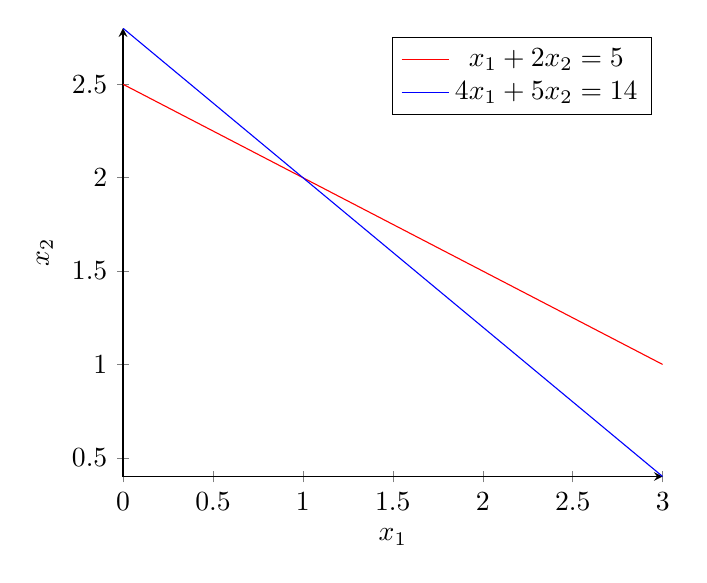
\begin{tikzpicture}
\begin{axis}[
    axis lines = left,
    xlabel = $x_1$,
    ylabel = {$x_2$},
]
%Below the red parabola is defined
\addplot [
    domain=0:3, 
    samples=100, 
    color=red,
]
{2.5-0.5*x};
\addlegendentry{$x_1+2x_2=5$}
%Here the blue parabloa is defined
\addplot [
    domain=0:3, 
    samples=100, 
    color=blue,
    ]
    {-0.8*x+2.8};
\addlegendentry{$4x_1+5x_2=14$}
\end{axis}
\end{tikzpicture}
\paragraph{Column Picture} Focusing on the column of the system of equation, we can denote 
$\begin{bmatrix}
1\\4
\end{bmatrix}$ and $\begin{bmatrix}
2\\5
\end{bmatrix}
$ as vectors in coordinate axis. {Could the linear combinations of these two vectors form the vector}
$\begin{bmatrix}
5\\14
\end{bmatrix}$?  If we denote $x_1$ and $x_2$ as coefficients, it suffices to solve the equation 
$
x_1\begin{bmatrix}
1\\4
\end{bmatrix} + x_2\begin{bmatrix}
2\\5
\end{bmatrix} = \begin{bmatrix}
5\\14
\end{bmatrix}$.

\subsubsection{The solutions of the Linear System of Equations}
The solution to linear system equation could only be \emph{unique}, \emph{infinite}, or \emph{empty}. Let's talk about it case by case in graphic way:
\paragraph{Case 1: unique solution} If two lines intersect at one point, then there is unique solution.
\begin{center}
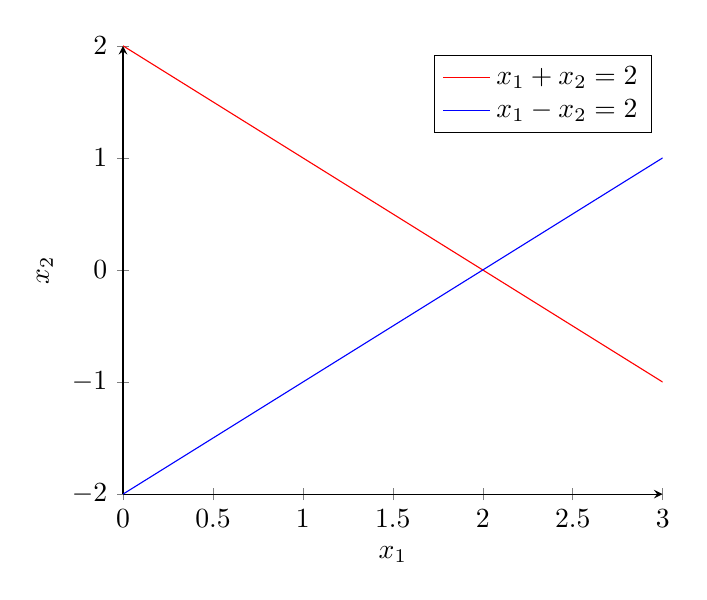
\begin{tikzpicture}
\begin{axis}[
    axis lines = left,
    xlabel = $x_1$,
    ylabel = {$x_2$},
]
%Below the red parabola is defined
\addplot [
    domain=0:3, 
    samples=100, 
    color=red,
]
{2-x};
\addlegendentry{$x_1+x_2=2$}
%Here the blue parabloa is defined
\addplot [
    domain=0:3, 
    samples=100, 
    color=blue,
    ]
    {x-2};
\addlegendentry{$x_1-x_2=2$}
\end{axis}
\end{tikzpicture}
\end{center}
\paragraph{Case2: no solution} If two lines are parallel, then there is no solution.
\begin{center}
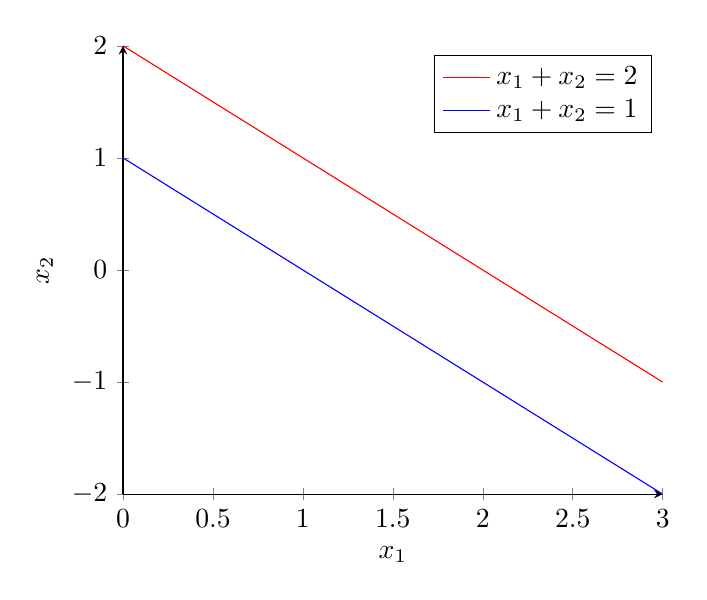
\begin{tikzpicture}
\begin{axis}[
    axis lines = left,
    xlabel = $x_1$,
    ylabel = {$x_2$},
]
%Below the red parabola is defined
\addplot [
    domain=0:3, 
    samples=100, 
    color=red,
]
{2-x};
\addlegendentry{$x_1+x_2=2$}
%Here the blue parabloa is defined
\addplot [
    domain=0:3, 
    samples=100, 
    color=blue,
    ]
    {1-x};
\addlegendentry{$x_1+x_2=1$}
\end{axis}
\end{tikzpicture}
\end{center}
\paragraph{Case 3: infinite number of solutions} If both equations represent the same line, then there are infinite number of solutions.
\begin{center}
\begin{tikzpicture}
\begin{axis}[
    axis lines = left,
    xlabel = $x_1$,
    ylabel = {$x_2$},
]
%Below the red parabola is defined
\addplot [
    domain=0:3, 
    samples=100, 
    color=red,
]
{2-x};
\addlegendentry{$x_1+x_2=2$}
%Here the blue parabloa is defined
\addplot [
    domain=0:3, 
    samples=100, 
    color=blue,
    ]
    {2-x};
\addlegendentry{$-x_1-x_2=-2$}
 
\end{axis}
\end{tikzpicture}
\end{center}
\subsubsection{How to solve $3 \times 3$ Systems?}

\begin{example} \qquad
\\
Let's recall how to solve a $3 \times 3$ system equations as below:

\[
\left \{	\begin{gathered}
2x_1 + x_2 +x_3=5 	\\
4x_1 + (-6)x_2 = -2 \\
-2x_2+7x_2+2x_3 = 9
\end{gathered}	\right.
\]
We can simplify the equation system above into the \emph{Augmented matrix} form:
\[
\left \{	\begin{gathered}
2x_1 + x_2 +x_3=5 	\\
4x_1 + (-6)x_2 = -2 \\
-2x_2+7x_2+2x_3 = 9
\end{gathered}	\right.
\qquad \implies \qquad
\left[
\begin{array}{@{}ccc|c@{}}
2 & 1 & 1 & 5\\
4 & -6 & 0 & -2\\
-2 & 7 & 2 & 9
\end{array}
\right]
\]
%
\[
\xLongrightarrow[\text{Add row 1 to row 3}]{\text{Add $(-2)\times$ row 1 to row 2}}{\quad\quad}
\left[
\begin{array}{@{}ccc|c@{}}
2 & 1 & 1 & 5\\
0 & -8 & -2 & -12\\
0 & 8 & 3 & 14
\end{array}
\right]
\]
\[\xLongrightarrow{\text{Add row 2 to row 3}}{\quad\quad}
\left[
\begin{array}{@{}ccc|c@{}}
2 & 1 & 1 & 5\\
0 & -8 & -2 & -12\\
0 & 0 & 1 & 2
\end{array}
\right]\]
This augmented matrix is the \emph{strictly triangular system}, and it's trial to get the final solution:
\[\implies
\begin{pmatrix}
x_1\\x_2\\x_3
\end{pmatrix}=
\begin{pmatrix}
1\\1\\2
\end{pmatrix}\]
\end{example}

Here we give the definition for strictly triangular system:
\begin{definition}[strictly triangular system]
For the augmented matrix
\[
\left[
\begin{array}{@{}cccc|c@{}}
a_{11} & a_{12} & \dots & a_{1n} &  b_1 \\
a_{21} & a_{22} & \dots & a_{2n} &  b_2 \\
\vdots    & \vdots    & \ddots & \vdots    & \vdots \\
a_{m1} & a_{m2} & \cdots & a_{mn} &   b_n
\end{array}
\right],
\]
if in the $k$th row, the first $(k-1)$th column entries are \textit{all zero} and the $k$th column entries is nonzero, we say the augmented matrix(or corresponding system equation) is of \emph{strictly triangular form}. This kind of matrix(or corresponding system equation) is called \emph{strictly triangular system}.
$(k = 1, . . . , m).$
\end{definition}

\subsubsection{How to solve $n \times n$ System?}
We try to reduce an $n \times n$ System to strictly triangular form. Let's take a special example:
\begin{example}
Given an $n \times n$ System of the form:
\begin{equation}\left[
\begin{array}{@{}cccc|c@{}}
a_{11} & a_{12} & \dots & a_{1n} &  b_1 \\
a_{21} & a_{22} & \dots & a_{2n} &  b_2 \\
\vdots    & \vdots    & \ddots & \vdots    & \vdots \\
a_{n1} & a_{n2} & \cdots & a_{nn} &   b_n
\end{array}\right]\label{eq:n*n_matrix}\end{equation}
Assuming the \emph{diagonal entries} are always \textit{nonzero} during our operation. 
Add row 1 that multiplied by a constant to other $n-1$ row to ensure the first entry of other $n-1$ rows are all \textit{zero}:
\begin{equation}
\implies 
\left[
\begin{array}{@{}cccc|c@{}}
a_{11} & a_{12} & \dots & a_{1n} &  b_1 \\
0 & \x & \dots & \x &  \x \\
\vdots    & \vdots    & \ddots & \vdots    & \vdots \\
0 & \x & \cdots & \x &   \x
\end{array}
\right] \label{eq:n*n_matrix_version1}\end{equation}


Then we proceed this way $n-1$times to obtain:
\begin{equation}
  \left[
    \begin{array}{@{}ccccc|c@{}}
    \x    & \x       & \x    & \x    & \x & \x\\ \cline{1-1}
    \bord & \x       & \x    & \x    & \x & \x\\ \cline{2-2}
          & \bord    & \x    & \x    & \x & \vdots \\ \cline{3-3}
          & \bigzero & \bord & \x    & \x & \vdots \\ \cline{4-4}
          &          &       & \bord & \x & \x \\ \cline{5-5}
  \end{array}\right]\label{eq:n*n_matrix_version2}
\end{equation}

This matrix is the \emph{Row-echelon form}.
And we do the back substitution again to obtain:
\begin{equation}
  \left[
    \begin{array}{@{}ccccc|c@{}}
    \x    &        &     &     &  & \x\\ \cline{1-1}
    \bord & \x       &     &     & \bigzero & \x\\ \cline{2-2}
          & \bord    & \x    &     &  & \vdots \\ \cline{3-3}
          & \bigzero & \bord & \x    &  & \vdots \\ \cline{4-4}
          &          &       & \bord & \x & \x \\ \cline{5-5}
  \end{array}\right]\label{eq:n*n_matrix_version3}
\end{equation}
This matrix is the \emph{Reduced Row-Echelon Form}.
Finally by multiplying every row by a nonzero constant to ensure its \emph{diagnoal entries} are all $1$:
\begin{equation}
  \left[
    \begin{array}{@{}ccccc|c@{}}
    1    &        &     &     &  & \x\\ \cline{1-1}
    \bord & 1       &     &     & \bigzero & \x\\ \cline{2-2}
          & \bord    & \ddots    &     &  & \vdots \\ \cline{3-3}
          & \bigzero & \bord & 1    &  & \vdots \\ \cline{4-4}
          &          &       & \bord & 1 & \x \\ \cline{5-5}
  \end{array}\right]\label{eq:n*n_matrix_version4}
\end{equation}
\end{example}

Then let's analysis the complexity of solving such a $n\times n$ system.
\subsection{Complexity Analysis}
\subsubsection{Step1: Reduction from matrix (\ref{eq:n*n_matrix}) to matrix (\ref{eq:n*n_matrix_version1})}
\begin{proposition}
The time complexity for Augmented matrix reduction using back-substitution algorithm is $\mathcal{O}(n^3)$.
\end{proposition}

\begin{proof}
The estimation for the time complexity requires us to estimate how many steps of \emph{multiplication} we need. (The time for addition is so small that can be ignored).
\begin{itemize}
\item
Reducing matrix (\ref{eq:n*n_matrix}) to matrix (\ref{eq:n*n_matrix_version1}) we need to do $n(n-1)$times multiplications.

This is because for each row (except first row) we have known the first entry is zero, while the remaining $(n-1)$ entries in each row should be computed by multiplying first row's entries and then add it to the row.
\item
Then it suffices to deal with the inner $(n-1)\times (n-1)$ matrix, which requires the $(n-1)\times (n-2)$ times multiplication.
\item
The back substitution for matrix (\ref{eq:n*n_matrix}) requires $n$ times reduction.
\end{itemize}
Hence the total multiplication times for back substitution for matrix (\ref{eq:n*n_matrix}) is
\begin{equation*}
\begin{split}
\sum_{i=1}^n i(i-1)
	&= \sum_{i=1}^n (i^2-i)  \\
 		&=\sum_{i=1}^n i^2 - \sum_{i=1}^n i \\
		&=\frac{n(n+1)(2n+1)}{6} - \frac{n(n+1)}{2} \\
		&=\frac{n^3-2n}{3} \sim \frac{n^3}{3} =O(n^3)
\end{split}
\end{equation*}
\end{proof}
But we can always develop more advanced algorithm that have smaller time complexity.

\subsubsection{Step2: Reduction from triangular system to diagonal system}

In order to reducing matrix (\ref{eq:n*n_matrix_version2}) to matrix (\ref{eq:n*n_matrix_version3}) we need to do back-substitution again. The matrix (\ref{eq:n*n_matrix_version3}) is diagonal system. Obviously, for this process the total multiplication times is given by
\[
1+2+\cdots+n-1 = \frac{n(n-1)}{2} \sim O(n^2)
\]
\subsubsection{Step3: Get final solution}

In the final step, we want to reduce matrix (\ref{eq:n*n_matrix_version3}) to matrix (\ref{eq:n*n_matrix_version4}), the only thing we need to do is to do one multiplication for each row to let the diagonal entries be $1$. Hence the total multiplication times for this process is given by
\[
\underbrace{1+1+\dots+1}_{\text{totally $n$ terms}} = O(n)
\]
\subsection{Brief Summary}
The reduction of $n\times n$ matrix requires three kinds of Row operations:
\begin{itemize}
\item \emph{Addition and Multiplication}.

Add to a row by a constant multiple of another row.

\item \emph{Multiplication}

Multiply a row by a nonzero constant.
\item \emph{Interchange}

Interchange two rows
\end{itemize}


\begin{enumerate}
\item
agds
\end{enumerate}•

\section{Thursday}\index{week5_Thursday_lecture}
\subsection{Orthogonality and Projection}
Two vectors are orthogonal if their inner product is zero:
\[
\bm u\perp\bm v
\Longleftrightarrow
\inp{\bm u}{\bm v}=0\qquad\text{(if $\bm u,\bm v\in\mathbb{R}^{n}$, then $\bm u\trans\bm v=0$.)}
\]
And orthogonality among vectors has an important property:
\begin{proposition}\qquad\\
If \emph{nonzero} vectors $v_1,\dots,v_k$ are mutually orthogonal (mutulally means $v_i\perp v_j$ for any $i\ne j$), then $\{v_1,\dots,v_k\}$ must be ind.
\end{proposition}
\begin{proof}
We only need to show that 
\[
\text{if }\alpha_1v_1+\dots+\alpha_kv_k=\bm 0,\qquad
\text{then }
\alpha_i=0\text{ for any $i\in\{1,2,\dots,k\}$.}
\]
\begin{itemize}
\item
We do inner product to show $\alpha_1$ must be zero:
\[
\begin{aligned}
\inp{v_1}{\alpha_1v_1+\dots+\alpha_kv_k}
&=\inp{v_1}{\bm 0}=0\\
&=\alpha_1\inp{v_1}{v_1}+\alpha_2\inp{v_1}{v_2}+\dots+\alpha_k\inp{v_1}{v_k}\\
&=\alpha_1\inp{v_1}{v_1}=\alpha_1\|v_1\|_2^2\\
&=0
\end{aligned}
\]
Since $v_1\ne \bm 0$, we have $\alpha_1=0$.
\item
Similarly, we have $\alpha_i=0$ for $i=1,\dots,k$.
\end{itemize}
\end{proof}
Now we can also talk about orthogonality among spaces:
\enlargethispage{2cm}
\begin{definition}[subspace orthogonality]
Two subspaces $\bm U$ and $\bm V$ of a vector space are \emph{orthogonal} if every vector $\bm u$ in $\bm U$ is \textit{perpendicular} to every vector $\bm v$ in $\bm V$:
\[
\text{\emph{Orthogonal subspaces}}\qquad
\bm u\perp\bm v\quad\forall\bm u\in\bm U,\bm v\in\bm V.
\]
\end{definition}
\begin{example}
Two walls look \textit{perpendicular} but they are not orthogonal subspaces! The meeting line is in both $\bm U$ and $\bm V$-and this line is not perpendicular to itself. Two planes (dimensions $2$ and $2$ in $\mathbb{R}^{3}$) cannot be orthogonal subspaces.\\
\begin{figure}[H]
\centering
\includegraphics{week5/orthogonality}
\caption{Orthogonality is impossible when $\dim\bm U+\dim\bm V>\dim(\bm U\cup\bm V)$}
\end{figure}
\end{example}
\begin{remark}
When a vector is in two orthogonal subspaces, it \textit{must} be zero. It is \emph{perpendicular} to
itself. 
\\The reason is clear: this vector $\bm u\in\bm U$ and $\bm u\in\bm V$, so $\inp{\bm u}{\bm u}=0$. It has to be zero vector.
\end{remark}
If two subspaces are perpendicular, their basis must be ind.
\begin{theorem}
Assume $\{u_1,\dots,u_k\}$ is the basis for $\bm U$, $\{v_1,\dots,v_l\}$ is the basis for $\bm V.$ If $\bm U\perp\bm V$ ($u_i\perp v_j$ for $\forall i,j$), then $u_1,u_2,\dots,u_k,v_1,v_2,\dots,v_l$ must be ind.
\end{theorem}
\begin{proof}
Suppose there exists $\{\alpha_1,\dots,\alpha_k\}$ and $\{\beta_1,\dots,\beta_l\}$ such that
\[
\alpha_1u_1+\dots+\alpha_ku_k+\beta_1v_1+\dots+\beta_lv_l=\bm 0
\]
then equibalently,
\[
\alpha_1u_1+\dots+\alpha_ku_k=-(\beta_1v_1+\dots+\beta_lv_l)
\]
Then we set $\bm w=\alpha_1u_1+\dots+\alpha_ku_k$, obviously, $\bm w\in\bm U$ and $\bm w\in\bm V$.\\ Hence it must be zero (This is due to remark above). Thus we have
\begin{gather*}
\alpha_1u_1+\dots+\alpha_ku_k=\bm 0\\
\beta_1v_1+\dots+\beta_lv_l=\bm 0.
\end{gather*}
Due to the independence, we have $\alpha_i=0$ and $\beta_j=0$ for $\forall i,j$. 
\end{proof}
\begin{corollary}
If $\{u_1,u_2,\dots,u_k,v_1,v_2,\dots,v_l\}\in\bm W$, then $\dim(\bm W)\ge\dim(\bm U)+\dim(\bm V)$.\\ Note that $\bm U\cup\bm V\subset\bm W$.
\end{corollary}
For subspaces $\bm U$ and $\bm V\in\mathbb{R}^{n}$, if $\mathbb{R}^{n}=\bm U\cup\bm V$, and moreover, $n=\dim(\bm U)+\dim(\bm V)$, then we say $\bm V$ is the \emph{orthogonal complement} of $\bm U$.
\begin{definition}[orthogonal complement]
For subspaces $\bm U$ and $\bm V\in\mathbb{R}^{n}$, if $\dim(\bm U)+\dim(\bm V)=n$ and $\bm U\perp\bm V$, then we say $\bm V$ is the \emph{orthogonal complement} of $\bm U$. And we denote $\bm V$ as $\bm U^{\perp}$.\\
Moreover, $\bm V=\bm U^{\perp}\Longleftrightarrow\bm V^{\perp}=\bm U$.
\end{definition}
\begin{example}
Suppose $\bm U\cup\bm V=\mathbb{R}^{3}$, $\bm U=\Span\{\bm e_1,\bm e_2\}$. If $\bm V$ is the orthogonal complement of $\bm U$, then $\bm V=\Span\{\bm e_3\}$. \\Moreover, $\bm U$ could also be expressed as $\Span\left\{\begin{pmatrix}
1\\1\\0
\end{pmatrix},\begin{pmatrix}
0\\1\\0
\end{pmatrix}\right\}$.
\end{example}
\emph{Example:}\\
Next let's show the nullspace is the orthogonal complement of the row space. (In $\mathbb{R}^{n}$).
Suppose $\bm A$ is a $m\times n$ matrix.
\begin{itemize}
\item
Firstly, we show $\dim(N(\bm A))+\dim(C(\bm A\trans))=\dim(N(\bm A)\cup C(\bm A\trans))=\dim(\mathbb{R}^{n})=n$:\\
We know $\dim(N(\bm A))=n-r$, where $r=\rank(\bm A)$. And $r=C(\bm A\trans))$.\\ Hence $\dim(N(\bm A))+\dim(C(\bm A\trans))=n$.
\item
Then we show $N(\bm A)\perp C(\bm A\trans)$:\\
For any $x\in N(\bm A)$, if we set $\bm A=\begin{bmatrix}
a_1\\a_2\\\vdots\\a_m
\end{bmatrix}$, then we obtain:
\[
\bm{Ax}=\begin{bmatrix}
a_1\\a_2\\\vdots\\a_m
\end{bmatrix}\begin{bmatrix}
\bm x
\end{bmatrix}=\begin{bmatrix}
0\\0\\\vdots\\0
\end{bmatrix}
\]
Hence \textit{every row has a zero product with} $x$. In other words, $\inp{a_i}{x}=0$ for $\forall i\in\{1,2,\dots,m\}$.\\
Hence for any $y=\sum_{i=1}^m\alpha_ia_i\in C(\bm A\trans)$, we obtain:
\[
\begin{aligned}
\inp{x}{y}&=\inp{y}{x}=\inp{\sum_{i=1}^m\alpha_ia_i}{x}\\
&=\sum_{i=1}^{m}\alpha_i\inp{a_i}{x}=0.
\end{aligned}
\]
Hence $x\perp y$ for $\forall x\in N(\bm A)$ and $y\in C(\bm A\trans)$.\\
\end{itemize}
Hence $N(\bm A)^{\perp}=C(\bm A\trans)$.\\
If we applying this equation to $\bm A\trans$, then we have $N(\bm A\trans)^{\perp}=C(\bm A)$. 
\enlargethispage{1cm}
\begin{theorem}[Fundamental theorem for linear alegbra, part 2]\qquad\\
\emph{$N(\bm A)$ is the orthogonal complement of the row space $C(\bm A\trans)$ (in $\mathbb{R}^{n}$).}\\
\emph{$N(\bm A\trans)$ is the orthogonal complement of the row space $C(\bm A)$ (in $\mathbb{R}^{m}$).}
\end{theorem}
\newpage
\begin{corollary}
$\bm{Ax}=\bm b$ is solvable if and only if $\bm y\trans\bm A=\bm 0$ implies $\bm y\trans\bm b$=0.
\end{corollary}
\begin{proof}\qquad\\
$\bm{Ax}=\bm b$ is solvable.
$\Longleftrightarrow$
$\bm b\in C(\bm A)$.
$\Longleftrightarrow$
$\bm b\in N(\bm A\trans)^{\perp}$\\
$\Longleftrightarrow$
$\bm y\trans\bm b=0$ for $\forall y\in N(\bm A\trans)$
$\Longleftrightarrow$
$\bm y\trans\bm A=\bm 0$ implies $\bm y\trans\bm b$=0.
\end{proof}
The Inverse Negative Propositions is more important:
\begin{corollary}
$\bm{Ax}=\bm b$ has no solution if and  and only if $\exists \bm y$ s.t. $\bm y\trans\bm A=0$ and $\bm y\trans\bm b\ne 0$.
\end{corollary}
\begin{remark}
\begin{theorem}\label{theorem_12.3}
$\bm{Ax}\ge\bm b$ has no solution if and only if $\exists \bm y\ge\bm 0$ such that $\bm y\trans\bm A=\bm 0$ and $\bm y\trans\bm b\ge \bm 0$.
\end{theorem}
$\bm y\trans\bm A=0$ requires exists one linear combination of the row space to be zero.
\begin{proof}[Necessity case.]
Suppose $\exists \bm y\ge\bm 0$ such that $\bm y\trans\bm A=\bm 0$ and $\bm y\trans\bm b\ge \bm 0$. And we assume there exists $x^{*}$ such that $\bm Ax^{*}\ge\bm b$. By postmultiplying $\bm y\trans$ we have 
\[\bm y\trans\bm Ax^{*}\ge\bm y\trans\bm b>\bm 0
\implies 
\bm 0>\bm 0.
\]
which is a contradiction!
\end{proof}
The complete proof for this theorem is not required in this course.
\end{remark}
\begin{example}
Given the system 
\begin{equation}
\begin{aligned}
x_1+x_2&\ge1\\
-x_1&\ge-1\\
-x_2&\ge2
\end{aligned}
\end{equation}
Eq(1)$\x$1+Eq(2)$\x$1+Eq(3)$\x$1 gives
\[
0\ge 2
\]
which is a contradiction!\\
So the key idea of theorem (\ref{theorem_12.3}) is to construct a linear combination of row space to let it become zero. Then if the right hand is larger than zero, then this system has no solution.
\end{example}
\begin{remark}
\begin{corollary}
If $\bm A=\bm A\trans$, then $N(\bm A\trans)^{\perp}=C(A)=C(\bm A\trans)=N(\bm A)$.
\end{corollary}
\begin{corollary}\label{corollary_12.5}
The system $\bm{Ax}=\bm b$ may not have a solution, but $\bm A\trans\bm A\bm x=\bm A\trans\bm b$ always have at least one solution for $\forall\bm b$.
\end{corollary}
\begin{proof}
Since $\bm A\trans\bm A$ is symmetric, we have $C(\bm A\trans\bm A)=C(\bm A\bm A\trans)$. You can check by yourself that $C(\bm A\bm A\trans)=C(\bm A\trans)$.
Hence $C(\bm A\trans\bm A)=C(\bm A\trans)$.\\
For any vector $\bm b$ we have $\bm A\trans\bm b\in C(\bm A\trans)\implies\bm A\trans\bm b\in C(\bm A\trans\bm A)$, which means there exists a linear combination of the columns of $\bm A\trans\bm A$ that equals to $\bm b$.\\
Equivalently, there exists a solution to $\bm A\trans\bm A\bm x=\bm A\trans\bm b$.
\end{proof}
\begin{corollary}\label{corollary_12.6}
$\bm A\trans\bm A$ is invertible if and only if columns of $\bm A$ are ind.
\end{corollary}
\begin{proof}
We have shown that $C(\bm A\trans\bm A)=C(\bm A\trans)$.\\ Hence $C(\bm A\trans\bm A)^{\perp}=C(\bm A\trans)^{\perp}\implies N(\bm A\trans\bm A)=N(\bm A)$.\\
$\bm A$ has ind. columns
$\Longleftrightarrow$
$N(\bm A)=\{\bm 0\}$
$\Longleftrightarrow$
$N(\bm A\trans\bm A)=\{\bm 0\}$
$\Longleftrightarrow$
$\bm A\trans\bm A$ is invertible.
\end{proof}
\end{remark}
\subsection{Least Squares Approximations}
$\bm{Ax}=\bm b$ often has no solution, if so, what should we do?\\
We cannot always get the error $\bm e=\bm b-\bm{Ax}$ down to zero, so we want to use least square method to minimize the error. In other words, our goal is to
\[
\min_{\bm x}\bm e^2=\min_{\bm x}\|\bm{Ax}-\bm b\|^2=\sum_{i=1}^{m}(a_i\trans\bm x-b_i)^2
\]
where $\bm A=\begin{bmatrix}
a_1\\a_2\\\vdots\\a_m
\end{bmatrix}$ and $\bm b=\begin{bmatrix}
b_1\\b_2\\\vdots\\b_m
\end{bmatrix}$.\\
The minimizer $\bm x$ is called \emph{linear least squares solution}.
\subsubsection{Matrix Calculus}
Firstly, you should know some basic calculus knowledge for matrix:
\begin{itemize}
\item
$\frac{\partial(f\trans g)}{\partial x}=\frac{\partial f(x)}{\partial x}g(x)+\frac{\partial g(x)}{\partial x}f(x)$
\end{itemize}
Example:
\begin{itemize}
\item
$\frac{\partial(a\trans \bm x)}{\partial \bm x}=a$
\item
$\frac{\partial(a\trans \bm A\bm x)}{\partial \bm x}=\frac{\partial((\bm A\trans a)\trans\bm x)}{\partial \bm x}=\bm A\trans a$
\item
$\frac{\partial(\bm A\bm x)}{\partial \bm x}=\bm A\trans$
\item
$\frac{\partial(\bm x\trans\bm A\bm x)}{\partial \bm x}=\bm A\bm x+\bm A\trans\bm x$
\end{itemize}
Thus, in order to minimize $\|\bm{Ax}-\bm b\|^2=(\bm{Ax}-\bm b)\trans(\bm{Ax}-\bm b)$, we only need to let its \emph{partial derivative} with respect to $\bm x$ to be \emph{zero.} (Since its second derivative is non-negative, we will talk about it in detail in other courses.) Hence we have
\[\begin{aligned}
\frac{\partial (\bm{Ax}-\bm b)\trans(\bm{Ax}-\bm b)}{\partial \bm x}&=\frac{\partial(\bm{Ax}-\bm b)}{\partial \bm x}(\bm{Ax}-\bm b)+\frac{\partial(\bm{Ax}-\bm b)}{\partial \bm x}(\bm{Ax}-\bm b)=2\frac{\partial(\bm{Ax}-\bm b)}{\partial \bm x}(\bm{Ax}-\bm b)\\
&=2(\frac{\partial(\bm A\bm x)}{\partial \bm x}-\frac{\partial(\bm b)}{\partial \bm x})(\bm{Ax}-\bm b)\\
&=2\bm A\trans(\bm{Ax}-\bm b)=\bm 0.
\end{aligned}
\]
Or equivalently, 
\[
\bm A\trans\bm{Ax}=\bm A\trans\bm b.
\]
According to corollary (\ref{corollary_12.5}), this equation always exists a solution. And this equation is called \emph{normal equation}.
\begin{theorem}\label{theorem_12.4}
The partial derivatives of $\|\bm{Ax}-\bm b\|^2$ are \emph{zero} when $\bm A\trans\bm{Ax}=\bm A\trans\bm b.$
\end{theorem}
\subsubsection{Fit a stright line}
Given a collection of data $(\bm x_i,y_i)$ for $i=1,\dots,m$, we can fit the model parameters:
\[
\left\{
\begin{aligned}
y_1&=a_0+a_1x_{1,1}+a_2x_{1,2}+\dots+a_nx_{1,n}+\varepsilon_1\\
y_2&=a_0+a_1x_{2,1}+a_2x_{2,2}+\dots+a_nx_{2,n}+\varepsilon_2\\
\vdots\\
y_m&=a_0+a_1x_{m,1}+a_2x_{m,2}+\dots+a_nx_{m,n}+\varepsilon_m
\end{aligned}
\right.
\]
Our fit line is 
\[
\hat y=a_0+a_1x_1+a_2x_2+\dots+a_nx_n
\]
In \textit{compact matrix form}, we have
\[
\begin{bmatrix}
y_1\\y_2\\\vdots\\y_n
\end{bmatrix}
=\begin{bmatrix}
1&x_{1,1}&x_{1,2}&\dots&x_{1,n}\\
1&x_{2,1}&x_{2,2}&\dots&x_{2,n}\\
\vdots&\vdots&&&\\
1&x_{m,1}&x_{m,2}&\dots&x_{m,n}\\
\end{bmatrix}\begin{bmatrix}
a_0\\a_1\\a_2\\\vdots\\a_{n}
\end{bmatrix}+\begin{bmatrix}
\varepsilon_1\\\varepsilon_2\\\vdots\\\varepsilon_m
\end{bmatrix}
\]
Or equivalently, we have 
\[
\bm y=\bm{Ax}+\bm \varepsilon
\]
where $\bm A =\begin{bmatrix}
1&x_{1,1}&x_{1,2}&\dots&x_{1,n}\\
1&x_{2,1}&x_{2,2}&\dots&x_{2,n}\\
\vdots&\vdots&&&\\
1&x_{m,1}&x_{m,2}&\dots&x_{m,n}\\
\end{bmatrix}_{m\times (n+1)}$, $\bm x=\begin{bmatrix}
a_0\\a_1\\a_2\\\vdots\\a_{n}
\end{bmatrix}_{(n+1)\times 1}$, $\bm \varepsilon=\begin{bmatrix}
\varepsilon_1\\\varepsilon_2\\\vdots\\\varepsilon_m
\end{bmatrix}_{m\times 1}$.\\
Our goal is to minimize $\|\hat{\bm y}-\bm y\|^2=\|\bm{Ax}-\bm y\|^2$. Then by theorem (\ref{theorem_12.4}), we only need to sovle $\bm A\trans\bm A\bm x=\bm A\trans\bm y$.
\subsection{Projections}
In corollary (\ref{corollary_12.6}), we know that if $\bm A$ has ind. columns, then $\bm A\trans\bm A$ is invertible. On this condition, the normal equation $\bm A\trans\bm A\bm x=\bm A\trans\bm b$ has unique solution $\bm x^{*}=(\bm A\trans\bm A)^{-1}\bm A\trans\bm b$.\\
Thus the error $\bm b-\bm A\bm x^{*}$ is minimum. And $\bm A\bm x^{*}=\bm A(\bm A\trans\bm A)^{-1}\bm A\trans\bm b$ \emph{approximately} equals to $\bm b$. \\
\begin{itemize}
\item
If $\bm b$ and $\bm{A}\bm x^{*}$ are exactly in the same space, then $\bm{A}\bm x^{*}=\bm b$.
\item
Otherwise, just as the Figure (\ref{figure_12.2}) shown, $\bm A\bm x^{*}$ is the projection of $\bm b$ to subspace $C(\bm A)$.
\end{itemize}
\begin{figure}[H]\centering
\includegraphics{week5/projection}
\caption{The projection of $\bm b$ onto a subspace $C(\bm A)$.}\label{figure_12.2}\end{figure}
\begin{definition}[Projection]
The projection of $\bm b$ onto the subspace $C(\bm A)$ is denoted as $\Proj_{C(\bm A)}(\bm b)$.
\end{definition}
\begin{definition}[Projection matrix]
Given $\bm A\bm x^{*}=\bm A(\bm A\trans\bm A)^{-1}\bm A\trans\bm b=\Proj_{C(\bm A)}(\bm b)$. Since $[\bm A(\bm A\trans\bm A)^{-1}\bm A\trans]\bm b$ is the projection of $\bm b$, we call $\bm P=\bm A(\bm A\trans\bm A)^{-1}\bm A\trans$ as \emph{projection matrix}.
\end{definition}
\begin{definition}[Idempotent]
Let $\bm A$ be a \emph{square} matrix that satisfies $\bm A=\bm A\bm A$, then $\bm A$ is called a \emph{idempotent} matrix.
\end{definition}
Let's show the projection matrix is \textit{idempotent}:\\
\[
\begin{aligned}
\bm P^{2}&=\bm A(\bm A\trans\bm A)^{-1}\bm A\trans\bm A(\bm A\trans\bm A)^{-1}\bm A\trans\\
&=\bm A(\bm A\trans\bm A)^{-1}(\bm A\trans\bm A)(\bm A\trans\bm A)^{-1}\bm A\trans\\
&=\bm A(\bm A\trans\bm A)^{-1}\bm A\trans=\bm P.
\end{aligned}
\]
\subsubsection{Observations}
\begin{itemize}
\item
If $\bm b\in C(\bm A)$, then $\exists \bm x$ s.t. $\bm{Ax}=\bm b$. Moreover, the projection of $\bm b$ is exactly $\bm b$:
\[
\begin{aligned}
\bm{Pb}&=\bm A(\bm A\trans\bm A)^{-1}\bm A\trans(\bm b)\\
&=\bm A(\bm A\trans\bm A)^{-1}\bm A\trans(\bm{Ax})\\
&=\bm A(\bm A\trans\bm A)^{-1}(\bm A\trans\bm A)\bm x\\
&=\bm{Ax}=\bm b.
\end{aligned}
\]
\item
Assume $\bm A$ has only one column, say, $\bm a$. Then we have
\[\begin{aligned}
\bm x^{*}&=(\bm A\trans\bm A)^{-1}\bm A\trans\bm b=\frac{\bm a\trans\bm b}{\bm a\trans\bm a}\\
\bm A\bm x^{*}&=\bm{Pb}=\bm A(\bm A\trans\bm A)^{-1}\bm A\trans(\bm b)=\frac{\bm a\trans\bm b}{\bm a\trans\bm a}\times\bm a=\frac{\bm a\trans\bm b}{\|\bm a\|^2}\times\bm a
\end{aligned}
\]
More interestingly, 
\[\frac{\bm a\trans\bm b}{\|\bm a\|^2}\times\bm a=\frac{\|\bm a\|\|\bm b\|\cos\theta}{\|\bm a\|^2}\times\bm a=\|\bm b\|\cos\theta\times\frac{\bm a}{\|\bm a\|}\]
which is the projection of $\bm b$ onto a line $\bm a$. (Shown in figure below.)
\begin{figure}[H]
\centering\includegraphics[width=10cm]{week5/projection_line}
\caption{The projection of $\bm b$ onto a line $\bm a$.}
\end{figure}
More generally, we can write the projection of $\bm b$ as:
\[
\Proj_{\bm a}(\bm b)=\frac{\inp{\bm a}{\bm b}}{\inp{\bm a}{\bm a}}\bm a
\]
Look at the figure above! The error is $\bm b-\Proj_{\bm a}(\bm b)$, which is obviously perpendicular to $\bm a$. And $\bm b-\Proj_{\bm a}(\bm b)\in\Span\{\bm a,\bm b\}$.\\
If we define $\bm b'=\bm b-\Proj_{\bm a}(\bm b)$, then it's easy to check $\Span\{\bm a,\bm b'\}=\Span\{\bm a,\bm b\}$ and $\bm a\perp\bm b'$. Hence we convert a basis to another basis such that the elements are orthogonal to each other. We will discuss it in detail in next lecture. 
\end{itemize}









% !TEX encoding = UTF-8 Unicode
\chapterimage{chapter_head_2.pdf} % Chapter heading image

%\chapter{Week1}

\section{Friday}\index{Friday_lecture}

\subsection{Matrix Multiplication}
\subsubsection{How to compute matrix multiplication quickly?}
\enlargethispage{1cm}
Given $m\times n$ matrix $\bm A$ and $n\times k$ matrix $\bm B$, then the result of $\bm{AB}$ should be a $m\times k$ matrix.\\
Let’s show a specific example:
\begin{example}
Given $4\times 3$ matrix $\bm A$ and $3\times 2$ matrix $\bm B$, then the result of $\bm{AB}$ should be a $4\times 2$ matrix:
\[
\bm{AB}=\begin{bmatrix}
1&2&3\\4&5&6\\7&8&9\\10&11&12
\end{bmatrix}\begin{bmatrix}
1&1\\1&0\\1&0
\end{bmatrix}=\begin{bmatrix}
\x&\x\\\x&\x\\\x&\x\\\x&\x
\end{bmatrix}_{4\x 2}.
\]
And the $(i,j)$th entry of the result should be the $i$th row of $\bm A$ multiply the $j$th
column of $\bm B$. In this example, the result has $4\x 2$ entries.\\
So we have to process such progress $4\x 2$ times to obtain the final result.\\
But we can try a more effecient method, we can calculate the \textit{entire row} of the result more
easily. For example,
\[
\left[\begin{array}{@{}ccc@{}}
\cellcolor{blue!20}1&\cellcolor{green!20}2&\cellcolor{red!20}3\\4&5&6\\7&8&9\\10&11&12
\end{array}\right]\left[\begin{array}{@{}cc@{}}
\rowcolor{blue!20}1&1\\
\rowcolor{green!20}1&0\\
\rowcolor{red!20}1&0
\end{array}\right]=
\left[\begin{array}{@{}cc@{}}
\rowcolor{black!20}6&1\\\x&\x\\\x&\x\\\x&\x
\end{array}\right].
\]
We should notice that \emph{the first row of the result is the linear combination of the row of
matrix $\bm B$, and the coefficients are entries of the first row of matrix $\bm A$:}
\[
\left[
\begin{array}{c@{}}
\cellcolor{blue!20}1
\end{array}
\right]\times
\left[\begin{array}{cc@{}}
\rowcolor{blue!20}1&1
\end{array}\right]
+
\left[
\begin{array}{c@{}}
\cellcolor{green!20}2
\end{array}
\right]\times
\left[\begin{array}{cc@{}}
\rowcolor{green!20}1&1
\end{array}\right]
+
\left[
\begin{array}{c@{}}
\cellcolor{red!20}3
\end{array}
\right]\times
\left[\begin{array}{cc@{}}
\rowcolor{red!20}1&1
\end{array}\right]=
\left[
\begin{array}{cc@{}}
\rowcolor{black!20}6&1
\end{array}
\right].
\]
On the other hand, we can calculate the \textit{entire column} of the result quickly:
\[
\left[\begin{array}{>{\columncolor{blue!20}}c>{\columncolor{green!20}}c>{\columncolor{red!20}}c@{}}
1&2&3\\4&5&6\\7&8&9\\10&11&12
\end{array}\right]\left[\begin{array}{cc@{}}
\cellcolor{blue!20}1&1\\
\cellcolor{green!20}1&0\\
\cellcolor{red!20}1&0
\end{array}\right]=
\left[\begin{array}{>{\columncolor{black!20}}cc@{}}
6&1\\\x&\x\\\x&\x\\\x&\x
\end{array}\right].
\]
\emph{The first column of the result is the linear combination of the column of matrix $\bm A$, and
the coefficients are entries of the first column of matrix $\bm B$:}
\[
\left[\begin{array}{>{\columncolor{blue!20}}c@{}}
1\\4\\7\\10
\end{array}\right]\left[\begin{array}{c@{}}
\cellcolor{blue!20}1
\end{array}\right]
+
\left[\begin{array}{>{\columncolor{green!20}}c@{}}
2\\5\\8\\11
\end{array}\right]\left[\begin{array}{c@{}}
\cellcolor{green!20}1
\end{array}\right]
+
\left[\begin{array}{>{\columncolor{red!20}}c@{}}
3\\6\\9\\12
\end{array}\right]\left[\begin{array}{c@{}}
\cellcolor{red!20}1
\end{array}\right]
=
\left[\begin{array}{>{\columncolor{red!20}}c@{}}
6\\15\\24\\33
\end{array}\right].
\]
You can do the remaining calculation by yourself, and the final result is given by:
\[
\bm{AB}=\begin{bmatrix}
1&2&3\\4&5&6\\7&8&9\\10&11&12
\end{bmatrix}_{4\x 3}\x\begin{bmatrix}
1&1\\1&0\\1&0
\end{bmatrix}_{3\x 2}=\begin{bmatrix}
6&1\\15&4\\24&7\\33&10
\end{bmatrix}_{4\x 2}.
\]
\end{example}
\subsection{Elementary Matrix}
So let’s review the concept for elementary matrix by an example:
\begin{remark}
It seems that we only talk about elementary matrix of type III instead of other types. So in
this course you can think there is \emph{only one} type of elementary matrix. This may contradict what
you see in the textbook.
\end{remark}
\begin{definition}[Elementary Matrix]
An elementary matrix $\bm E_{ij}$ is a matrix that its \textit{diagonal entries} are all $1$ and the $(i,j)$th column is a \textit{scalar}, and the remaining entries are all \textit{zero}.
\end{definition}
For example, the matrix $\bm A=\begin{pmatrix}
1&0&0\\0&1&0\\4&0&1
\end{pmatrix}$ is elementary matrix.
\begin{example}
Given vector $\bm b=\begin{bmatrix}
b_1&b_2&b_3
\end{bmatrix}\trans$ and elementary matrix $\bm E_{31}=\begin{bmatrix}
1&0&0\\0&1&0\\-l_{31}&0&1
\end{bmatrix}$, the effct of \textit{postmultiplying} $\bm E_{31}$ has the same effect of doing row operation:
\[
\bm E_{31}\bm b=\begin{bmatrix}
b_1\\b_2\\b_3-l_{31}b_1
\end{bmatrix}
\]
Let’s do more practice, given matrix $\bm E_{21}=\begin{bmatrix}
1&0&0\\-l_{21}&1&0\\0&0&1
\end{bmatrix}$, we can calculate the result of $\bm E_{21}\x(\bm E_{31}\bm b)$ and $\bm E_{21}\bm E_{31}$:
\begin{gather*}
\bm E_{21}\x(\bm E_{31}\bm b)=\begin{bmatrix}
1&0&0\\-l_{21}&1&0\\0&0&1
\end{bmatrix}\times\begin{bmatrix}
b_1\\b_2\\b_3-l_{31}b_1
\end{bmatrix}=\begin{bmatrix}
b_1\\b_2-l_{21}b_1\\b_3-l_{31}b_1
\end{bmatrix}\\
\bm E_{21}\bm E_{31}=\begin{bmatrix}
1&0&0\\-l_{21}&1&0\\0&0&1
\end{bmatrix}\begin{bmatrix}
1&0&0\\0&1&0\\-l_{31}&0&1
\end{bmatrix}
=\begin{bmatrix}
1&0&0\\-l_{21}&1&0\\-l_{31}&0&1
\end{bmatrix}
\end{gather*}
And additionally, we can use matrix multiplication to derive the result of $(\bm E_{21}\bm E_{31})\times\bm b$:
\[
(\bm E_{21}\bm E_{31})\times\bm b=\begin{bmatrix}
1&0&0\\-l_{21}&1&0\\-l_{31}&0&1
\end{bmatrix}\begin{bmatrix}
b_1\\b_2\\b_3
\end{bmatrix}=\begin{bmatrix}
b_1\\b_2-l_{21}b_1\\b_3-l_{31}b_1
\end{bmatrix}
\]
\end{example}
Amazingly, we find the result of $\bm E_{21}\x(\bm E_{31}\bm b)$ is actually the same as $(\bm E_{21}\bm E_{31})\times\bm b$, which is one of the properties of matrix.
\subsection{Properties of Matrix}
Operations on matrix has the following properties:
\begin{enumerate}
\item
$\bm A(\bm B+\bm C)=\bm{AB}+\bm{AC}.$
\item
$\bm{AB}\ne\bm{BA}$, this means $\bm{AB}$ doesn’t \textit{necessarily} equal to $\bm{BA}$.
\begin{remark}
In some special cases, $\bm{AB}$ may equal to $\bm{BA}$. For example, for elementary matrix, we have $\bm E_{21}\bm E_{31}=\bm E_{31}\bm E_{21}$, this means the order of row operation can be changed sometimes.\\\\
However, for most cases the equality is not satisfied. given row vector $\bm a=\begin{bmatrix}
a_1&a_2&a_3
\end{bmatrix}$ and column vector $\bm b=\begin{pmatrix}
b_1\\b_2\\b_3
\end{pmatrix}$, the result of $\bm{ab}$ and $\bm{ba}$ is given by:
\begin{gather*}
\bm{ab}=\begin{pmatrix}
a_1&a_2&a_3
\end{pmatrix}\begin{pmatrix}
b_1\\b_2\\b_3
\end{pmatrix}=a_1b_1+a_2b_2+a_3b_3\\
\bm{ba}=\begin{pmatrix}
b_1\\b_2\\b_3
\end{pmatrix}\begin{pmatrix}
a_1&a_2&a_3
\end{pmatrix}=\begin{pmatrix}
b_1a_1&b_1a_2&b_1a_3\\
b_2a_1&b_2a_2&b_2a_3\\
b_3a_1&b_3a_2&b_3a_3
\end{pmatrix}.
\end{gather*}
\end{remark}
\item
\emph{Block Multiplication} 
We use an example to show the process of block multiplicaion:
\begin{example}
Given two matrix $\bm A$ and $\bm B$, and we obtain $\bm A\x\bm B=\bm C$. In order to
compute the result of $\bm C$, we can partition $\bm A$ and $\bm B$ arbitrarily, for example, 
\[
\bm A=\left[
\begin{array}{@{}cc|c@{}}
4&0&4\\
6&6&8\\
\hline
-9&5&-8
\end{array}
\right]
=\begin{bmatrix}
\bm A_1&\bm A_2\\\bm A_3&\bm A_4
\end{bmatrix},\qquad
\bm B=\left[
\begin{array}{@{}cc|c@{}}
8&-3&-7\\
3&-7&-4\\
\hline
4&-4&1
\end{array}
\right]=\begin{bmatrix}
\bm B_1&\bm B_2\\\bm B_3&\bm B_4
\end{bmatrix}.
\]
The entries in $\bm A$ and $\bm B$ are picked arbitrarily. Thus we partition $\bm C$ into $4$ blocks
respectively:
\[
\bm C=\bm{AB}=\begin{bmatrix}
\bm C_1&\bm C_2\\\bm C_3&\bm C_4
\end{bmatrix}
\]
And there is an effective way to calculate $\bm C_1$, that is the block multiplication method
shown below:
\begin{gather*}
\bm{AB}=\begin{bmatrix}
\bm A_1&\bm A_2\\\bm A_3&\bm A_4
\end{bmatrix}\begin{bmatrix}
\bm B_1&\bm B_2\\\bm B_3&\bm B_4
\end{bmatrix}=\begin{bmatrix}
\bm{A_1B_1}+\bm{A_2B_3}&\bm{A_1B_2}+\bm{A_2B_4}\\\bm{A_3B_1}+\bm{A_4B_3}&\bm{A_3B_2}+\bm{A_4B_4}
\end{bmatrix}
=\begin{bmatrix}
\bm C_1&\bm C_2\\\bm C_3&\bm C_4
\end{bmatrix}\\
\implies
\bm C_1=\bm{A_1B_1}+\bm{A_2B_3}
=\begin{bmatrix}
4&0\\6&6
\end{bmatrix}\begin{bmatrix}
8&-3\\3&-7
\end{bmatrix}+\begin{bmatrix}
4\\-8
\end{bmatrix}\begin{bmatrix}
4&-4
\end{bmatrix}=\begin{bmatrix}
48&-28\\34&-28
\end{bmatrix}.
\end{gather*}
And you can do the remaining calculation to get result of $\bm{AB}$:
\[
\bm{AB}=\bm C=\left[\begin{array}{@{}cc|c@{}}
48&-28&-24\\34&-28&-74\\-89&24&35
\end{array}\right]
\]
\end{example}
And if we know $\bm B$ has $k$ columns, we can partition $\bm B$ into $k$ blocks to compute $\bm{AB}$:
\[
\bm{AB}=\bm A\x
\left[
\begin{array}{@{}c|c|c|c@{}}
B_1&B_2&\dots&B_k
\end{array}\right]
=\left[
\begin{array}{@{}c|c|c|c@{}}
\bm AB_1&\bm AB_2&\dots&\bm AB_k
\end{array}\right].
\]
Also, if we know $\bm A$ has $m$ rows, we can partition $\bm A$ into $m$ blocks to compute $\bm{AB}$:
\[
\bm{AB}=\left[\begin{array}{@{}c@{}}
\bm A_1\\
\hline
\bm A_2\\
\hline
\dots\\
\hline
\bm A_{m}
\end{array}\right]\x\bm B
=\left[\begin{array}{@{}c@{}}
\bm A_1\bm B\\
\hline
\bm A_2\bm B\\
\hline
\dots\\
\hline
\bm A_{m}\bm B
\end{array}\right]
\]
\end{enumerate}
\subsection{Permutation Matrix}
We notice that there is one type of matrix $\bm P$ such that postmultiplying $\bm P$ for arbitararily matrix $\bm A$ has the same effect of interchanging two rows of $\bm A$.\\
For example, if $\bm P=\begin{bmatrix}
0&1\\1&0
\end{bmatrix},$ $\bm A=\begin{bmatrix}
1&2\\3&4
\end{bmatrix},$ by postmultiplying $\bm P$ for $\bm A$ we obtain:
\[
\bm{PA}=\begin{bmatrix}
0&1\\1&0
\end{bmatrix}\begin{bmatrix}
1&2\\3&4
\end{bmatrix}=\begin{bmatrix}
3&4\\1&2
\end{bmatrix}.
\]
This progress has the same effect of interchanging the first row and the second row of $\bm A$.\\
This kind of matrix is called \textit{permutaion matrix}:
\begin{definition}[Permutation Matrix]\qquad\\
$\bm P$ is a \emph{permutation matrix} if postmultiplying $\bm P$ for matrix $\bm A$ has the same effect of interchanging rows of matrix $\bm A$.
\end{definition}
But how to describle a matrix that exchanges row $i$ and row $j$? We use notation $\bm P_{ij}$ to denote such
matrix. A matrix that only interchange two rows is called \textit{row exchange matrix}:
\begin{definition}[Row Exchange Matrix]
After a identity matrix’s $i$th and $j$th row being exchanged, it is denoted by $\bm P_{ij}$. And $\bm P_{ij}$ is called \emph{Row Exchange Matrix}. By postmultiplying $\bm P_{ij}$ for matrix $\bm A$ has the same effect of interchanging row $i$ and row $j$ of matrix $\bm A$.
\end{definition}
Let’s raise some examples to show what is row exchange matrix:
\begin{example}
$\bm P_{23}$ is used to exchange row $2$ and row $3$ of arbitarary matrix. And it is converted from identity matrix:
\begin{gather*}
\bm I=\begin{bmatrix}
1&0&0\\0&1&0\\0&0&1
\end{bmatrix}
\xLongrightarrow{\text{Interchange row $2$ and $3$}}
\begin{bmatrix}
1&0&0\\0&0&1\\0&1&0
\end{bmatrix}=\bm P_{23}.\\
\bm I=\begin{bmatrix}
1&0&0&0\\0&1&0&0\\0&0&1&0\\0&0&0&1
\end{bmatrix}
\xLongrightarrow{\text{Interchange row $2$ and $3$}}
\begin{bmatrix}
1&0&0&0\\0&0&1&0\\0&1&0&0\\0&0&0&1
\end{bmatrix}=\bm P_{23}.
\end{gather*}
Postmultiplying by $\bm P_{23}$ exchanges row $2$ and row $3$ of any matrix:
\[
\begin{bmatrix}
1&0&0\\0&0&1\\0&1&0
\end{bmatrix}
\left[
\begin{array}{cc@{}}
6&7\\
\rowcolor{blue!20}
15&4\\
\rowcolor{green!20}
24&3
\end{array}
\right]=
\left[
\begin{array}{cc@{}}
6&7\\
\rowcolor{green!20}
24&3\\
\rowcolor{blue!20}
15&4
\end{array}
\right]
\qquad\text{and}\qquad
\begin{bmatrix}
1&0&0&0\\0&1&0&0\\0&0&1&0\\0&0&0&1
\end{bmatrix}
\left[
\begin{array}{c@{}}
6\\
\rowcolor{green!20}
24\\
\rowcolor{blue!20}
15\\
4
\end{array}\right]
=\left[
\begin{array}{c@{}}
6\\
\rowcolor{blue!20}
15\\
\rowcolor{green!20}
24\\
4
\end{array}\right]
\]
\end{example}
\begin{remark}
You may be confused about the concept between \textit{permutation matrix} and \textit{row exchange matrix.} Our $\bm P_{23}$ (row exchange matrix) is just one particular permutation matrix---it exchanges
row 2 and row 3. Soon we will meet other permutation matrix, which can change the order of \emph{several} rows. For example, rows 1,2,3 can be changed to 3,2,1.
\end{remark}
Before we talk about the properties of permutation matrix, let’s introduce the definition for
nonsingular and inverse matrix:
\begin{definition}[Nonsigular matrix]
Let $\bm A$ be an $n\x n$ matrix, the following statements are equivalent:
\begin{enumerate}
\item
$\bm A$ is \emph{nonsingular} or \emph{invertible}.
\item
There exists a matrix $\bm B$ such that $\bm{AB}=\bm{BA}=\bm I$. And the matrix $\bm B$ is said to be the \emph{inverse} of $\bm A$, and we can write $\bm B=\bm A^{-1}.$
\item
After multiplying finite numbers of \emph{elementary matrix}, $\bm A$ can be converted to identity matrix $\bm I.$
\item
The system of equations $\bm{Ax}=\bm b$ has a unique solution.
\end{enumerate}
If matrix $\bm A$ is \emph{not} nonsingular, this matrix is called \emph{singular}.
\end{definition}
And we are interested in the form of the inverse of permutation matrix.
\begin{proposition}
\begin{enumerate}
\item
For a permutation matrix $\bm P$, it can always be decomposed into finite multiplication of row
exchange matrix $\bm P_{ij}$:
\[
\bm P=\bm P_{i_1j_1}\bm P_{i_2j_2}\ldots\bm P_{i_nj_n}
\]
\item
The inverse of a row exchange matrix is actually equal to itself:
\[
\bm P_{ij}\bm P_{ij}=\bm I
\Longleftrightarrow
\bm P_{ij}^{-1}=\bm P_{ij}
\]
\item
For a permutation matrix written as $\bm P=\bm P_{i_1j_1}\bm P_{i_2j_2}\ldots\bm P_{i_nj_n},$ its inverse matrix is given by:
\[
\bm P^{-1}=\bm P_{i_nj_n}^{-1}\bm P_{i_{n-1}j_{n-1}}^{-1}\ldots\bm P_{i_1j_1}^{-1}
=\bm P_{i_nj_n}\bm P_{i_{n-1}j_{n-1}}\ldots\bm P_{i_1j_1}
\]
\item
For $n\x n$ permutation matrix and $n\x n$ matrix given by
\[
\bm P=\left[\begin{array}{@{}c|ccc@{}}
1&0&0&0\\
\hline
0&&&\\
\vdots&&\bm P_{(n-1)\x(n-1)}&\\
0&&&
\end{array}\right]\qquad
\bm A=\left[\begin{array}{@{}c|ccc@{}}
a_{11}&a_{12}&\dots&a_{1n}\\
\hline
0&&&\\
\vdots&&\bm A_{(n-1)\x(n-1)}&\\
0&&&
\end{array}\right]
\]
we have:
\[
\bm P\bm A=\left[\begin{array}{@{}c|ccc@{}}
a_{11}&a_{12}&\dots&a_{1n}\\
\hline
0&&&\\
\vdots&&\bm P_{(n-1)\x(n-1)}\bm A_{(n-1)\x(n-1)}&\\
0&&&
\end{array}\right]
\]
\end{enumerate}
\end{proposition}
\begin{proof}[Proofoutline.]\qquad\\
\begin{itemize}
\item
For proposition $2$, it is because that if we exchange two rows of any matrix $\bm A$, and then we
exchange the same rows again, the effect is nothing!
\item
For proposition 3, it is because that we just need to do reverse order of our process in order to
get the inverse matrix.
\end{itemize}
\end{proof}
\subsection{LU decomposition}
After learning matrix multiplication, we should be familiar some basic result of matrix multiply
matrix:
\begin{enumerate}
\item
\emph{Product of upper triangular matries is also upper triangular matrix.}
\[
\left[
    \begin{array}{@{}ccccc@{}}
    \x    & \x       & \x    & \x    & \x \\ \cline{1-1}
    \bord & \x       & \x    & \x    & \x \\ \cline{2-2}
          & \bord    & \x    & \x    & \x \\ \cline{3-3}
          & \bigzero & \bord & \x    & \x \\ \cline{4-4}
          &          &       & \bord & \x \\ \cline{5-5}
  \end{array}\right]
  \left[
    \begin{array}{@{}ccccc@{}}
    \x    & \x       & \x    & \x    & \x \\ \cline{1-1}
    \bord & \x       & \x    & \x    & \x \\ \cline{2-2}
          & \bord    & \x    & \x    & \x \\ \cline{3-3}
          & \bigzero & \bord & \x    & \x \\ \cline{4-4}
          &          &       & \bord & \x \\ \cline{5-5}
  \end{array}\right]
  =
  \left[
    \begin{array}{@{}ccccc@{}}
    \x    & \x       & \x    & \x    & \x \\ \cline{1-1}
    \bord & \x       & \x    & \x    & \x \\ \cline{2-2}
          & \bord    & \x    & \x    & \x \\ \cline{3-3}
          & \bigzero & \bord & \x    & \x \\ \cline{4-4}
          &          &       & \bord & \x \\ \cline{5-5}
  \end{array}\right].
\]
\item
\emph{Product of diagonal matrices is also diagonal matrix.}
\[
\left[
    \begin{array}{@{}ccccc@{}}
    d_1    &        &     &     &  \\ \cline{1-1}
    \bord & d_2       &     & \bigzero    &  \\ \cline{2-2}
          & \bord    & \ddots    &     &  \\ \cline{3-3}
          & \bigzero & \bord & \ddots    &  \\ \cline{4-4}
          &          &       & \bord & d_n \\ \cline{5-5}
  \end{array}\right]
  \left[
    \begin{array}{@{}ccccc@{}}
    e_1    &        &     &     &  \\ \cline{1-1}
    \bord & e_2       &     & \bigzero    &  \\ \cline{2-2}
          & \bord    & \ddots    &     &  \\ \cline{3-3}
          & \bigzero & \bord & \ddots    &  \\ \cline{4-4}
          &          &       & \bord & e_n \\ \cline{5-5}
  \end{array}\right]
  =
  \left[
    \begin{array}{@{}ccccc@{}}
    d_1e_1    &        &     &     &  \\ \cline{1-1}
    \bord & d_2e_2       &     & \bigzero    &  \\ \cline{2-2}
          & \bord    & \ddots    &     &  \\ \cline{3-3}
          & \bigzero & \bord & \ddots    &  \\ \cline{4-4}
          &          &       & \bord & d_ne_n \\ \cline{5-5}
  \end{array}\right].
\]
\end{enumerate}
And like permutation matrix, there are also some intersting properties of elementary matrix:
\begin{proposition}
\item
The inverse of a elementary matrix is also a elementary matrix.\\
For example, $\bm E_{21}=\begin{bmatrix}
1&0&0\\-2&1&0\\0&0&1
\end{bmatrix}$ is an elementary matrix, the result of postmultiplying identity matrix is given by:
\[
\bm E_{21}\bm I=\begin{bmatrix}
1&0&0\\-2&1&0\\0&0&1
\end{bmatrix}
\]
It has the same effect of adding $(-2)\x$ row $1$ to row $2$. How to get identity again? We just need to add $2\x$ row $1$ to row $2$. So we only need to postmultiply another elementary matrix:
\[
\overline{\bm E_{21}}\bm E_{21}\bm I=\overline{\bm E_{21}}\bm E_{21}=\overline{\bm E_{21}}\begin{bmatrix}
1&0&0\\-2&1&0\\0&0&1
\end{bmatrix}
=\begin{bmatrix}
1&0&0\\2&1&0\\0&0&1
\end{bmatrix}\begin{bmatrix}
1&0&0\\-2&1&0\\0&0&1
\end{bmatrix}
=\begin{bmatrix}
1&0&0\\0&1&0\\0&0&1
\end{bmatrix}=\bm I.
\]
Hence $\overline{\bm E_{21}}$ is the inverse matrix of $\bm E_{21}$.
\item
The product of elementary matrix $\bm E_{ij}$ $(i<j)$ is lower triangular matrix. The product of
elementary matrix $\bm E_{ij}$ $(i>j)$ is upper triangular matrix.
\end{proposition}
Let’s look at an example to see what is LU decomposition:
\begin{example}
Let’s try Gaussian Elimination for a matrix that is nonsingular. Here we use elementary matrix to describle row operation above the arrow (without row exchange):
\[
\bm A=\begin{bmatrix}
2&1&1\\4&-6&0\\-2&7&2
\end{bmatrix}\xLongrightarrow{\bm E_{21}}
\begin{bmatrix}
2&1&1\\0&-8&-2\\-2&7&2
\end{bmatrix}\xLongrightarrow{\bm E_{31}}
\begin{bmatrix}
2&1&1\\0&-8&-2\\0&8&3
\end{bmatrix}\xLongrightarrow{\bm E_{32}}
\begin{bmatrix}
2&1&1\\0&-8&-2\\0&0&1
\end{bmatrix}=\bm U
\]
In this process we have $\bm E_{21}=\begin{bmatrix}
1&0&0\\-2&1&0\\0&0&1
\end{bmatrix},\quad\bm E_{31}=\begin{bmatrix}
1&0&0\\0&1&0\\1&0&1
\end{bmatrix},\quad\bm E_{32}=\begin{bmatrix}
1&0&0\\0&1&0\\0&1&1
\end{bmatrix}$.\\
Finally we convert $\bm A$ into an upper triangular matrix $\bm U$. Let’s reverse the process to find some interesting conclusion:
\begin{gather*}
\bm E_{32}\bm E_{31}\bm E_{21}\bm A=\bm U\\
\implies
\bm E_{32}^{-1}\bm E_{32}\bm E_{31}\bm E_{21}\bm A=\bm E_{32}^{-1}\bm U\\
\implies
\bm E_{31}\bm E_{21}\bm A=\bm E_{32}^{-1}\bm U\\
\cdots\implies
\bm A=\bm E_{21}^{-1}\bm E_{31}^{-1}\bm E_{32}^{-1}\bm U=\bm{LU}.
\end{gather*}
where $\bm L=\bm E_{21}^{-1}\bm E_{31}^{-1}\bm E_{32}^{-1}$, which is lower triangular matrix.\\
And we successfully decompose matrix $\bm A$ into multiplication of a lower triangular matrix $\bm L$
and a upper triangular matrix $\bm U$.
\end{example}
\subsubsection{One Square System = Two Triangular Systems}
When considering the \textit{nonsingular} case without row exchanges, recall what we have done before this lecture: we are working on $\bm A$ and $\bm b$ in one equation $\bm{Ax}=\bm b$. But computer wants to deal with $\bm A$ and $\bm b$ in separate equations. So LU decomposition can help us do the following things:
\begin{enumerate}
\item
\emph{Decomposition:} By elimination on matrix $\bm A$, we can decompose $\bm A$ into two matrix multiplication: $\bm A=\bm{LU}.$
\item
\emph{Solve:} forward elimination on $\bm b$ using $\bm L$, then back substitution for $\bm x$ using $\bm U$.
\begin{remark}
\textit{How does Solve work on?} First, we apply forward elimination to $\bm b$, which changes $\bm b$ to $\bm y$. In other words, we are actually solving $\bm{Ly}=\bm b$. After getting $\bm y$, we then do
back substitution to solve $\bm{Ux}=\bm y$. In other words, in second step we are solving $\bm{Ux}=\bm y$. The original system $\bm{Ax}=\bm b$ is converted into two triangular systems:
\[
\text{\emph{Forward and Backward}}\qquad
\text{Solve $\bm{Ly}=\bm b$ and then solve $\bm{Ux}=\bm y$.}
\]
\end{remark}
\begin{remark}
There is nothing new about those steps. This is exactly what we have done all the time. We are really solving the triangular system $\bm{Ly}=\bm b$ as elimination went forward. Then back substitution produced $\bm x$. An example shows what we actually
did:
\begin{example}
Forward elimination on $\bm{Ax}=\bm b$ will result in equation $\bm{Ux}=\bm y$:
\[
\bm{Ax}=\bm b\Longleftrightarrow
\left\{
\begin{aligned}
u+2v&=5\\4u+9v&=21
\end{aligned}
\right\}
\qquad
\text{becomes}
\left\{
\begin{aligned}
u+2v&=5\\v&=1
\end{aligned}
\right\}
\Longleftrightarrow
\bm{Ux}=\bm y.
\]
\textit{How to use matrix to compute it more quickly?}
\begin{itemize}
\item
$\bm{Ly}=\bm b:$\qquad In this system of equation, we know $\bm L=\begin{bmatrix}
1&0\\4&1
\end{bmatrix},$ in oder to solve
$\bm y$, we only need to multiply the inverse of $\bm L$ both sides:
\[
\begin{bmatrix}
1&0\\4&1
\end{bmatrix}\x\bm y=\begin{bmatrix}
5\\21
\end{bmatrix}\implies
\bm y=\bm L^{-1}\begin{bmatrix}
5\\21
\end{bmatrix}=\begin{bmatrix}
1&0\\-4&1
\end{bmatrix}\begin{bmatrix}
5\\21
\end{bmatrix}=\begin{bmatrix}
5\\1
\end{bmatrix}.
\]
\newpage
\item
$\bm{Ux}=\bm y:$\qquad In this system of equation, we know $\bm U=\begin{bmatrix}
1&2\\0&1
\end{bmatrix},$ in oder to solve
$\bm x$, we only need to multiply the inverse of $\bm U$ both sides:
\[
\begin{bmatrix}
1&2\\0&1
\end{bmatrix}\x\bm x=\begin{bmatrix}
5\\1
\end{bmatrix}\implies
\bm x=\bm U^{-1}\begin{bmatrix}
5\\1
\end{bmatrix}=\begin{bmatrix}
1&-2\\0&1
\end{bmatrix}\begin{bmatrix}
5\\1
\end{bmatrix}=\begin{bmatrix}
3\\1
\end{bmatrix}.
\]
Both \emph{Forward} and \emph{Back substitution} has $O(n^2)$ time complexity.
\end{itemize}
\end{example}
\end{remark}
\end{enumerate}
\subsection{LDU decomposition}
Suppose we have decomposed $\bm A$ into $\bm{LU}$, and the upper triangular matrix $\bm U$ is given by:
\[
\left[
    \begin{array}{@{}ccccc@{}}
    d_1    & \x       & \x    & \x    & \x \\ \cline{1-1}
    \bord & d_2       & \x    & \x    & \x \\ \cline{2-2}
          & \bord    & d_3    & \x    & \x \\ \cline{3-3}
          & \bigzero & \bord & d_4    & \x \\ \cline{4-4}
          &          &       & \bord & d_5 \\ \cline{5-5}
  \end{array}\right]
\]
If we want to let its diagonal entries to be all \emph{one}, we just need to multiply a matrix $\bm D^{-1}$ that is
given by:
\[
\left[
    \begin{array}{@{}ccccc@{}}
    d_1^{-1}    &        &     &     &  \\ \cline{1-1}
    \bord & d_2^{-1}       &    &  \bigzero   &  \\ \cline{2-2}
          & \bord    & d_3^{-1}    &     &  \\ \cline{3-3}
          & \bigzero & \bord & d_4^{-1}    &  \\ \cline{4-4}
          &          &       & \bord & d_5^{-1} \\ \cline{5-5}
  \end{array}\right]
\implies
\bm D^{-1}\bm U=
\left[
    \begin{array}{@{}ccccc@{}}
    1    & \x       & \x    & \x    & \x \\ \cline{1-1}
    \bord & 1       & \x    & \x    & \x \\ \cline{2-2}
          & \bord    & 1    & \x    & \x \\ \cline{3-3}
          & \bigzero & \bord & 1    & \x \\ \cline{4-4}
          &          &       & \bord & 1 \\ \cline{5-5}
  \end{array}\right].
\]
And we can translate LU decomposition into LDU decomposition by multiplying factor $\bm D\bm D^{-1}$:
\[
\bm A=\bm L\bm U=\bm L\bm D\bm D^{-1}\bm U
=\bm L\bm D(\bm D^{-1}\bm U)
=\bm L\bm D\overline{\bm U},
\]
where $\overline{\bm U}=\bm D^{-1}\bm U$ is also an upper triangular matix.\\
Since we know exactly matrix $\bm D^{-1}$, we can
solve for matrix $\bm D$:
\[
\bm D=\left[
    \begin{array}{@{}ccccc@{}}
    d_1    &        &     &     &  \\ \cline{1-1}
    \bord & d_2       &    &  \bigzero   &  \\ \cline{2-2}
          & \bord    & d_3    &     &  \\ \cline{3-3}
          & \bigzero & \bord & d_4    &  \\ \cline{4-4}
          &          &       & \bord & d_5 \\ \cline{5-5}
  \end{array}\right]
\]
In order to verify this solution you just need to multiply it by $\bm D^{-1}$ to ensure its result to be
\textit{identity matrix}. And we notice that the \textit{diagonal} entries of $\bm D$ are all \textit{pivots values} of $\bm U$.\\
Similarly, we can proceed this step again to let \textit{diagonal} entries of $\bm L$ to be $1$.
In conclusion, we decompose matrix $\bm A$ into the form:
\begin{align*}
\bm A&=\bm L\bm D\bm U\\
\text{where }&\text{$\bm L$ is lower triangular matrix with unit entries in diagonal}\\
&\text{$\bm D$ is diagonal matrix}\\
&\text{$\bm U$ is upper triangular matrix with unit entries in diagonal}
\end{align*}
This decomposition is called \emph{LDU decomposition}. Here is a property of LDU decomposition,
we state it first without proof. We will proof it in the future.
\begin{proposition}
Let $\bm L$ be a lower triangular matrix, $\bm D$ diagonal, and $\bm U$ upper triangular. If
$\bm A=\bm{LDU}$ and also $\bm A=\bm L_1\bm D_1\bm U_1$, then we have $\bm L=\bm L_1,\bm D=\bm D_1,\bm U=\bm U_1$. In other words, \emph{LDU
decomposition is unique to any matrix.}
\end{proposition}
\subsection{LU Decomposition with row exchanges}
How can we handle row exchange in our $\bm{LU}$ decomposition? \\
Assume we are going to do
Gaussian Elimination with matrix $\bm A$. We can postmultiply many elementary matrix $\bm E$ to get
$\bm{EEEA}$. Sometimes we need to multiply by $\bm P_{ij}$ to do \textit{row exchange} to continue Gaussian
Elimination. So we may end our elimination with something like $\bm{PEEEEPEEEPEEEEA}$. If
we can get all the elementary matrix $\bm L$ together, we could convert them into one single $\bm L$ that has
the same effect as before. \\But \textit{how can we get all the row exchange matrix $\bm P$ out from among
the $\bm L$?}\\
\begin{theorem}
If $\bm A$ is \textit{nonsingular}, then there exists a permutation matrix $\bm P$ such that $\bm{PA}=\bm{LU}$.
\end{theorem}
We skip the proof of this theorem, if you are interested in it, you may check the website:
\begin{verbatim}
http://www.doc88.com/p-9387269167515.html
\end{verbatim}
\include{week1/Assignment_One}
%\include{week2/Lecture_1}
%\include{week2/Lecture_2}

\chapter{Week1}

\section{Tuesday}\index{Tuesday_lecture}

\subsection{Introduction}
\subsubsection{\textit{Why do you learn Linear Algebra?}}
\paragraph{Important: LA + Calculus + Probability}

Every SSE student should learn {\emph{Linear Algebra}}, {\emph{Calculus}}, and {\emph{Probability}} to build strong fundation.

\paragraph{Practical: Computation}

Linear Algebra is more widely used than Calculus since we could use this {\emph{powerful}} tool to do discrete computation. (As we know, we can use calculus to deal with something continuous. But how do we do integration when facing lots of \emph{discrete data}? But linear algebra can help us deal with these data.)

\paragraph{Visualize} 

Conncect between \emph{Geometry} and \emph{Algebra}.

Let's take an easy example:
\begin{example}

Let $v$ and $w$ donate two vectors as below:
\[
\begin{array}{ll}
v= \begin{bmatrix}
1 \\ 2
\end{bmatrix},
&
w = \begin{bmatrix}
3 \\ 4
\end{bmatrix}.
\end{array}
\]

Then we can donate these two vectors in the graph:
\begin{center}
\setlength{\unitlength}{0.5 cm}
\begin{picture}(15,3)\thicklines
\put(0,0){\vector(1,2){1}} \put(0,0){\vector(1,0){2}}
\put(-0.2,1){$v$} \put(1,-0.6){$w$} \put(3.2,2){$v+w$}
\put(1,2){\line(1,0){0.2}} \put(0,0){\vector(3,2){3}}
\put(1.4,2){\line(1,0){0.2}} \put(1.8,2){\line(1,0){0.2}}
\put(2.2,2){\line(1,0){0.2}} \put(2.6,2){\line(1,0){0.2}}
\put(8,1){\vector(1,1){2}} \put(8,1){\vector(2,-1){2}}
\put(10,0){\vector(0,1){3}} \put(8.3,1.9){$v$} \put(8.3,0){$w$}
\put(10.5,1){$v-w$}
\end{picture}
\end{center}

And we can also add two vectors to get $v+w$. Additionally, we can change the coefficients in front of $v$ and $w$ to get $v-w$.

In two dimension space, we can visualize the vector in the coordinate. Then let's watch the \emph{three} dimension space.There are four vectors $u$,$v$,$w$ and $b$. We can also denote it in coordinate.

Here we raise a question: Can we denote vector $b$ as a linear combination with the three vectors $u$, $v$, and $w$? That is to say,
\begin{quotation}
Is there exists coefficients $x_1$, $x_2$, $x_3$ such that 
\[
x_1 \begin{pmatrix}
1 \\ 1 \\ 1
\end{pmatrix}+
x_2 \begin{pmatrix}
1 \\ 2 \\ 3
\end{pmatrix}+
x_3 \begin{pmatrix}
1 \\ 3 \\ 4
\end{pmatrix}=
\begin{pmatrix}
2 \\ 5 \\ 7
\end{pmatrix}?
\]
\end{quotation}

Then we only need to solve the system of equations 
\[\left\{ \begin{gathered}
x_1 + x_2 + x_3 = 2 \\
x_1 + 2x_2 + 3x_3 = 5 \\
x_1 + 3x_2 + 4x_3 = 7
\end{gathered} \right.
\implies \begin{pmatrix}
x_1 \\ x_2 \\ x_3
\end{pmatrix} = \begin{pmatrix}
0 \\ 1 \\ 1
\end{pmatrix}
\]
\end{example}
\paragraph{Abstract: Broad Applications}

Don't worry, broad doesn't mean boring. Instead, it means Linear Algebra can applied to lots of applications.

For example, if we denote a sequence of infinite numbers as a tuple that contains infinite numbers, and we denote this tuple as a vector, then we could build \emph{an infinite banach space.} Moreover, Given a function $f:\mathbb{R} \to \mathbb{R}$, we can describle a set of functions as a tuple, then we could build a \emph{function space}. These abstract knowledge may be not covered in this course. We will learn it in future courses.

\subsubsection{What is Linear Algebra?}
The central problem in math is to \emph{solve equations}. And equations can be seperated into two parts, \emph{nonlinear} and \emph{linear} ones. 

Let's look an example of Nonlinear equations below:
\[ 
\left\{ \begin{gathered}
3x_1x_2 + 5x_1^2 + 6x_2 = 9 \\
x_1x_2^2 + 5x_1 + 7x_2^2 = 10
\end{gathered}
\right.
\]

Well, it is a little bit complicated. We don't find a efficient algorithm to solve these equations. But in algebraic geometry course we will solve some nonlinear equations.

What you need to know about in this course is the linear equations and the methodology to solve it.

\begin{definition}[Linear Equations]
A linear equation in $n$ unknowns is the equation of the form
\[
a_1x_1 + a_2x_2 +\dots + a_nx_n = b,
\]
where $a_1,a_2,\dots,a_n,b$ are real numbers and $x_1,x_2,\dots,x_n$ are variables
\end{definition}

\begin{definition}[Linear System of Equations]
Linear system of $m$ equations in $n$ unknowns is the system of the form

\begin{gather}
a_{11}x_1 + a_{12}x_2 + \dots + a_{1n}x_n = b_1 \notag \\ 
a_{21}x_1 + a_{22}x_2 + \dots + a_{23}x_n = b_2 \notag \\
\dots 	\notag 	\\
a_{m1}x_1 + a_{m2}x_2 + \dots + a_{m3}x_n = b_m , \label{Eq:1.1}
\end{gather}
where $a_{ij}$ and the $b_i$ are all real numbers. We refer to (\ref{Eq:1})as $m \times n$ \emph{linear systems}.
\end{definition}

 
%------------------------------------------------

\subsection{Gaussian Elimination}

Here we mainly focus on $n \times n$ system of equations. 

\begin{example}
Let's recall how to solve a $2 \times 2$ system equatons as below:
\begin{align}
1x_1 + 2x_2 &= 5\label{Eq:1.2}\\
4x_1 + 5x_2 &=14\label{Eq:1.3}.
\end{align}

We can simplify the equation system above into the form (\emph{Augmented matrix}):
\[
\left[
\begin{array}{@{}cc|c@{}}
1 & 2 & 5 \\
4 & 5 & 14
\end{array}
\right]
\]

Secondly, by adding $(-4)\times(\ref{Eq:1.2})$ into (\ref{Eq:1.3}), we obtain:
\begin{align}
{1}x_1 + 2x_2 &=5\label{Eq:1.4}\\
0x_1 + (-3)x_2 &= -6\label{Eq:1.5}
\end{align}

Thirdly, by multiplying $-(1/3)$ of (\ref{Eq:1.5}), we obtain:
\begin{align}
{1}x_1 + 2x_2 &=5 \label{Eq:1.6}\\
1x_2 &= 2\label{Eq:1.7}
\end{align}

Fourthly, by adding $(-2)\times(\ref{Eq:1.7})$ into $(\ref{Eq:1.6})$, we obtain:
\begin{align}
{1}x_1 + 0x_2 &=1 	\\
1x_2 &= 2 
\end{align}

Here we get the solution $(x_1=1, x_2=2)$, and we could write the above process with augmented matrix form:
\[
\left[
\begin{array}{@{}cc|c@{}}
1 & 2 & 5 \\
4 & 5 & 14
\end{array}
\right]
\implies
\left[
\begin{array}{@{}cc|c@{}}
1 & 2 & 5 \\
0& -3 & -6
\end{array}
\right]
\implies
\left[
\begin{array}{@{}cc|c@{}}
1 & 2 & 5 \\
0& 1 & 2
\end{array}
\right]
\implies
\left[
\begin{array}{@{}cc|c@{}}
1 & 0 & 1 \\
0& 1 & 2
\end{array}
\right].
\]
\end{example}

The method shown above is called \emph{Gaussian Elimination}. Here we give a strict definition for Augmented matrix:
\begin{definition}[Augmented matrix]
For the system of equations
\begin{gather}
a_{11}x_1 + a_{12}x_2 + \dots + a_{1n}x_n = b_1 \notag \\ 
a_{21}x_1 + a_{22}x_2 + \dots + a_{2n}x_n = b_2 \notag \\
\dots 	\notag 	\\
a_{m1}x_1 + a_{m2}x_2 + \dots + a_{mn}x_n = b_m , \label{eq:linear system equations_2}
\end{gather}
the corresponding augmented matrix is given by 
\[
\left[
\begin{array}{@{}cccc|c@{}}
a_{11} & a_{12} & \dots & a_{1n} &  b_1 \\
a_{21} & a_{22} & \dots & a_{2n} &  b_2 \\
\vdots    & \vdots    & \ddots & \vdots    & \vdots \\
a_{m1} & a_{m2} & \cdots & a_{mn} &   b_n
\end{array}
\right].
\]
\end{definition}

We give the definition for a new term \emph{pivot}:
\begin{definition}[pivot]
Returning to the example, we find after third step the matrix is given by 
\[
\left[
\begin{array}{@{}cc|c@{}}
1 & 2 & 5 \\
0 & 1 & 2
\end{array}
\right].
\]

We find that the second row will be used to eliminate the element in the second column of the first row. Here we refer to the second row as the \emph{pivot
row}. The first nonzero entry in the pivotal row is called the \emph{pivot}. For the example case, the element in the second column of the second row is the pivot.
\end{definition}

\subsubsection{How to visualize the system of equation?}
Here we try to visualize the system of equation $
\left \{	\begin{gathered}
1x_1 + 2x_2 =5	\\
4x_1 + 5x_2 = 14 
\end{gathered}	\right.$:

\paragraph{Row Picture} Focusing on the row of the system of equation, we can denote each equation as a line on the coordinate axis. And the solution denote the coordinate.

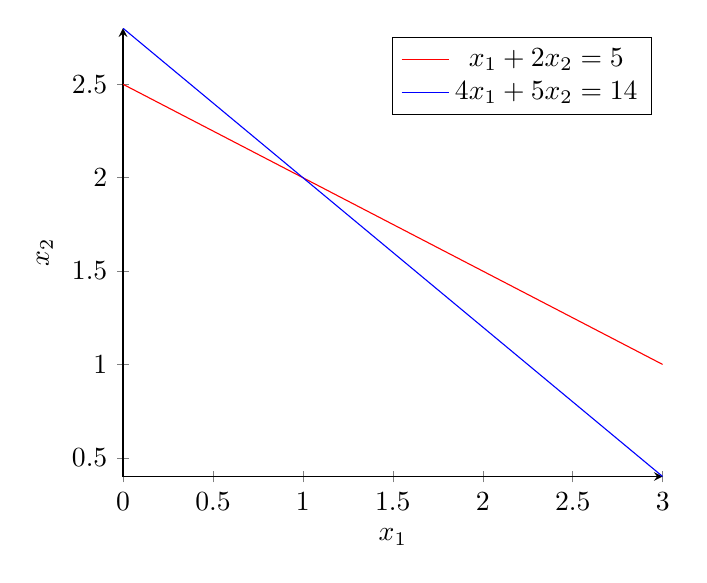
\begin{tikzpicture}
\begin{axis}[
    axis lines = left,
    xlabel = $x_1$,
    ylabel = {$x_2$},
]
%Below the red parabola is defined
\addplot [
    domain=0:3, 
    samples=100, 
    color=red,
]
{2.5-0.5*x};
\addlegendentry{$x_1+2x_2=5$}
%Here the blue parabloa is defined
\addplot [
    domain=0:3, 
    samples=100, 
    color=blue,
    ]
    {-0.8*x+2.8};
\addlegendentry{$4x_1+5x_2=14$}
\end{axis}
\end{tikzpicture}
\paragraph{Column Picture} Focusing on the column of the system of equation, we can denote 
$\begin{bmatrix}
1\\4
\end{bmatrix}$ and $\begin{bmatrix}
2\\5
\end{bmatrix}
$ as vectors in coordinate axis. {Could the linear combinations of these two vectors form the vector}
$\begin{bmatrix}
5\\14
\end{bmatrix}$?  If we denote $x_1$ and $x_2$ as coefficients, it suffices to solve the equation 
$
x_1\begin{bmatrix}
1\\4
\end{bmatrix} + x_2\begin{bmatrix}
2\\5
\end{bmatrix} = \begin{bmatrix}
5\\14
\end{bmatrix}$.

\subsubsection{The solutions of the Linear System of Equations}
The solution to linear system equation could only be \emph{unique}, \emph{infinite}, or \emph{empty}. Let's talk about it case by case in graphic way:
\paragraph{Case 1: unique solution} If two lines intersect at one point, then there is unique solution.
\begin{center}
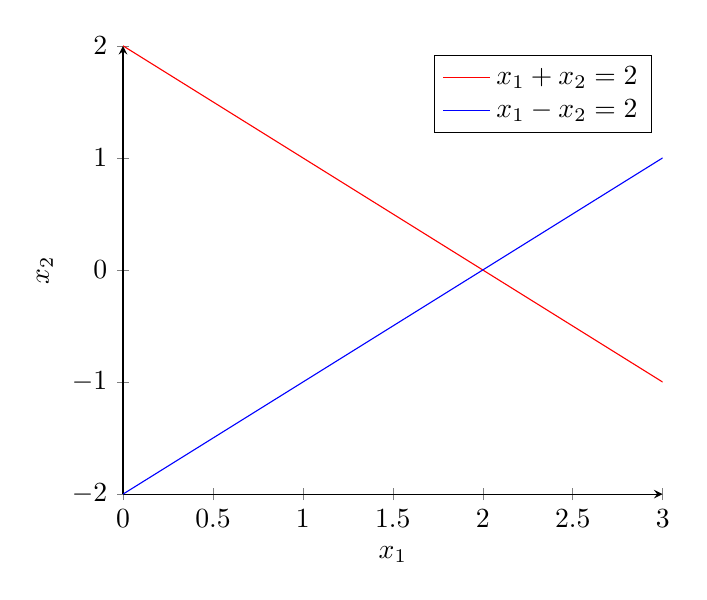
\begin{tikzpicture}
\begin{axis}[
    axis lines = left,
    xlabel = $x_1$,
    ylabel = {$x_2$},
]
%Below the red parabola is defined
\addplot [
    domain=0:3, 
    samples=100, 
    color=red,
]
{2-x};
\addlegendentry{$x_1+x_2=2$}
%Here the blue parabloa is defined
\addplot [
    domain=0:3, 
    samples=100, 
    color=blue,
    ]
    {x-2};
\addlegendentry{$x_1-x_2=2$}
\end{axis}
\end{tikzpicture}
\end{center}
\paragraph{Case2: no solution} If two lines are parallel, then there is no solution.
\begin{center}
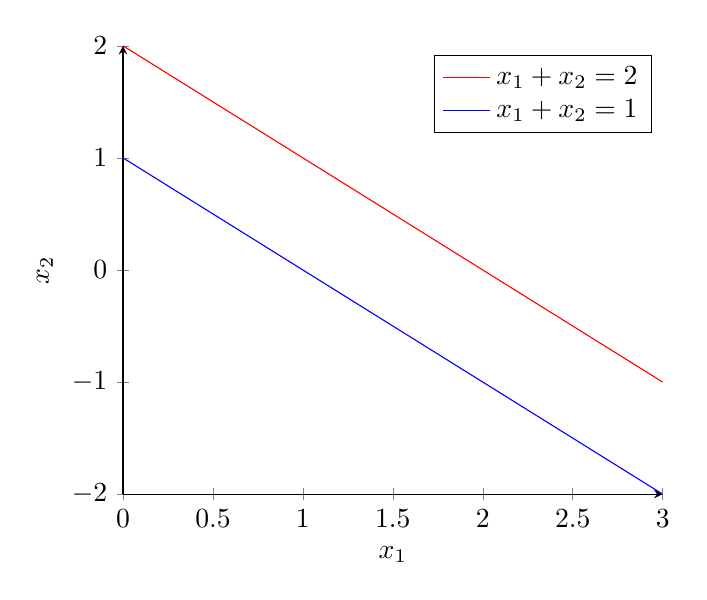
\begin{tikzpicture}
\begin{axis}[
    axis lines = left,
    xlabel = $x_1$,
    ylabel = {$x_2$},
]
%Below the red parabola is defined
\addplot [
    domain=0:3, 
    samples=100, 
    color=red,
]
{2-x};
\addlegendentry{$x_1+x_2=2$}
%Here the blue parabloa is defined
\addplot [
    domain=0:3, 
    samples=100, 
    color=blue,
    ]
    {1-x};
\addlegendentry{$x_1+x_2=1$}
\end{axis}
\end{tikzpicture}
\end{center}
\paragraph{Case 3: infinite number of solutions} If both equations represent the same line, then there are infinite number of solutions.
\begin{center}
\begin{tikzpicture}
\begin{axis}[
    axis lines = left,
    xlabel = $x_1$,
    ylabel = {$x_2$},
]
%Below the red parabola is defined
\addplot [
    domain=0:3, 
    samples=100, 
    color=red,
]
{2-x};
\addlegendentry{$x_1+x_2=2$}
%Here the blue parabloa is defined
\addplot [
    domain=0:3, 
    samples=100, 
    color=blue,
    ]
    {2-x};
\addlegendentry{$-x_1-x_2=-2$}
 
\end{axis}
\end{tikzpicture}
\end{center}
\subsubsection{How to solve $3 \times 3$ Systems?}

\begin{example} \qquad
\\
Let's recall how to solve a $3 \times 3$ system equations as below:

\[
\left \{	\begin{gathered}
2x_1 + x_2 +x_3=5 	\\
4x_1 + (-6)x_2 = -2 \\
-2x_2+7x_2+2x_3 = 9
\end{gathered}	\right.
\]
We can simplify the equation system above into the \emph{Augmented matrix} form:
\[
\left \{	\begin{gathered}
2x_1 + x_2 +x_3=5 	\\
4x_1 + (-6)x_2 = -2 \\
-2x_2+7x_2+2x_3 = 9
\end{gathered}	\right.
\qquad \implies \qquad
\left[
\begin{array}{@{}ccc|c@{}}
2 & 1 & 1 & 5\\
4 & -6 & 0 & -2\\
-2 & 7 & 2 & 9
\end{array}
\right]
\]
%
\[
\xLongrightarrow[\text{Add row 1 to row 3}]{\text{Add $(-2)\times$ row 1 to row 2}}{\quad\quad}
\left[
\begin{array}{@{}ccc|c@{}}
2 & 1 & 1 & 5\\
0 & -8 & -2 & -12\\
0 & 8 & 3 & 14
\end{array}
\right]
\]
\[\xLongrightarrow{\text{Add row 2 to row 3}}{\quad\quad}
\left[
\begin{array}{@{}ccc|c@{}}
2 & 1 & 1 & 5\\
0 & -8 & -2 & -12\\
0 & 0 & 1 & 2
\end{array}
\right]\]
This augmented matrix is the \emph{strictly triangular system}, and it's trial to get the final solution:
\[\implies
\begin{pmatrix}
x_1\\x_2\\x_3
\end{pmatrix}=
\begin{pmatrix}
1\\1\\2
\end{pmatrix}\]
\end{example}

Here we give the definition for strictly triangular system:
\begin{definition}[strictly triangular system]
For the augmented matrix
\[
\left[
\begin{array}{@{}cccc|c@{}}
a_{11} & a_{12} & \dots & a_{1n} &  b_1 \\
a_{21} & a_{22} & \dots & a_{2n} &  b_2 \\
\vdots    & \vdots    & \ddots & \vdots    & \vdots \\
a_{m1} & a_{m2} & \cdots & a_{mn} &   b_n
\end{array}
\right],
\]
if in the $k$th row, the first $(k-1)$th column entries are \textit{all zero} and the $k$th column entries is nonzero, we say the augmented matrix(or corresponding system equation) is of \emph{strictly triangular form}. This kind of matrix(or corresponding system equation) is called \emph{strictly triangular system}.
$(k = 1, . . . , m).$
\end{definition}

\subsubsection{How to solve $n \times n$ System?}
We try to reduce an $n \times n$ System to strictly triangular form. Let's take a special example:
\begin{example}
Given an $n \times n$ System of the form:
\begin{equation}\left[
\begin{array}{@{}cccc|c@{}}
a_{11} & a_{12} & \dots & a_{1n} &  b_1 \\
a_{21} & a_{22} & \dots & a_{2n} &  b_2 \\
\vdots    & \vdots    & \ddots & \vdots    & \vdots \\
a_{n1} & a_{n2} & \cdots & a_{nn} &   b_n
\end{array}\right]\label{eq:n*n_matrix}\end{equation}
Assuming the \emph{diagonal entries} are always \textit{nonzero} during our operation. 
Add row 1 that multiplied by a constant to other $n-1$ row to ensure the first entry of other $n-1$ rows are all \textit{zero}:
\begin{equation}
\implies 
\left[
\begin{array}{@{}cccc|c@{}}
a_{11} & a_{12} & \dots & a_{1n} &  b_1 \\
0 & \x & \dots & \x &  \x \\
\vdots    & \vdots    & \ddots & \vdots    & \vdots \\
0 & \x & \cdots & \x &   \x
\end{array}
\right] \label{eq:n*n_matrix_version1}\end{equation}


Then we proceed this way $n-1$times to obtain:
\begin{equation}
  \left[
    \begin{array}{@{}ccccc|c@{}}
    \x    & \x       & \x    & \x    & \x & \x\\ \cline{1-1}
    \bord & \x       & \x    & \x    & \x & \x\\ \cline{2-2}
          & \bord    & \x    & \x    & \x & \vdots \\ \cline{3-3}
          & \bigzero & \bord & \x    & \x & \vdots \\ \cline{4-4}
          &          &       & \bord & \x & \x \\ \cline{5-5}
  \end{array}\right]\label{eq:n*n_matrix_version2}
\end{equation}

This matrix is the \emph{Row-echelon form}.
And we do the back substitution again to obtain:
\begin{equation}
  \left[
    \begin{array}{@{}ccccc|c@{}}
    \x    &        &     &     &  & \x\\ \cline{1-1}
    \bord & \x       &     &     & \bigzero & \x\\ \cline{2-2}
          & \bord    & \x    &     &  & \vdots \\ \cline{3-3}
          & \bigzero & \bord & \x    &  & \vdots \\ \cline{4-4}
          &          &       & \bord & \x & \x \\ \cline{5-5}
  \end{array}\right]\label{eq:n*n_matrix_version3}
\end{equation}
This matrix is the \emph{Reduced Row-Echelon Form}.
Finally by multiplying every row by a nonzero constant to ensure its \emph{diagnoal entries} are all $1$:
\begin{equation}
  \left[
    \begin{array}{@{}ccccc|c@{}}
    1    &        &     &     &  & \x\\ \cline{1-1}
    \bord & 1       &     &     & \bigzero & \x\\ \cline{2-2}
          & \bord    & \ddots    &     &  & \vdots \\ \cline{3-3}
          & \bigzero & \bord & 1    &  & \vdots \\ \cline{4-4}
          &          &       & \bord & 1 & \x \\ \cline{5-5}
  \end{array}\right]\label{eq:n*n_matrix_version4}
\end{equation}
\end{example}

Then let's analysis the complexity of solving such a $n\times n$ system.
\subsection{Complexity Analysis}
\subsubsection{Step1: Reduction from matrix (\ref{eq:n*n_matrix}) to matrix (\ref{eq:n*n_matrix_version1})}
\begin{proposition}
The time complexity for Augmented matrix reduction using back-substitution algorithm is $\mathcal{O}(n^3)$.
\end{proposition}

\begin{proof}
The estimation for the time complexity requires us to estimate how many steps of \emph{multiplication} we need. (The time for addition is so small that can be ignored).
\begin{itemize}
\item
Reducing matrix (\ref{eq:n*n_matrix}) to matrix (\ref{eq:n*n_matrix_version1}) we need to do $n(n-1)$times multiplications.

This is because for each row (except first row) we have known the first entry is zero, while the remaining $(n-1)$ entries in each row should be computed by multiplying first row's entries and then add it to the row.
\item
Then it suffices to deal with the inner $(n-1)\times (n-1)$ matrix, which requires the $(n-1)\times (n-2)$ times multiplication.
\item
The back substitution for matrix (\ref{eq:n*n_matrix}) requires $n$ times reduction.
\end{itemize}
Hence the total multiplication times for back substitution for matrix (\ref{eq:n*n_matrix}) is
\begin{equation*}
\begin{split}
\sum_{i=1}^n i(i-1)
	&= \sum_{i=1}^n (i^2-i)  \\
 		&=\sum_{i=1}^n i^2 - \sum_{i=1}^n i \\
		&=\frac{n(n+1)(2n+1)}{6} - \frac{n(n+1)}{2} \\
		&=\frac{n^3-2n}{3} \sim \frac{n^3}{3} =O(n^3)
\end{split}
\end{equation*}
\end{proof}
But we can always develop more advanced algorithm that have smaller time complexity.

\subsubsection{Step2: Reduction from triangular system to diagonal system}

In order to reducing matrix (\ref{eq:n*n_matrix_version2}) to matrix (\ref{eq:n*n_matrix_version3}) we need to do back-substitution again. The matrix (\ref{eq:n*n_matrix_version3}) is diagonal system. Obviously, for this process the total multiplication times is given by
\[
1+2+\cdots+n-1 = \frac{n(n-1)}{2} \sim O(n^2)
\]
\subsubsection{Step3: Get final solution}

In the final step, we want to reduce matrix (\ref{eq:n*n_matrix_version3}) to matrix (\ref{eq:n*n_matrix_version4}), the only thing we need to do is to do one multiplication for each row to let the diagonal entries be $1$. Hence the total multiplication times for this process is given by
\[
\underbrace{1+1+\dots+1}_{\text{totally $n$ terms}} = O(n)
\]
\subsection{Brief Summary}
The reduction of $n\times n$ matrix requires three kinds of Row operations:
\begin{itemize}
\item \emph{Addition and Multiplication}.

Add to a row by a constant multiple of another row.

\item \emph{Multiplication}

Multiply a row by a nonzero constant.
\item \emph{Interchange}

Interchange two rows
\end{itemize}


\begin{enumerate}
\item
agds
\end{enumerate}•
\chapterimage{chapter_head_2.pdf} % Chapter heading image

%\chapter{Week2}

\section{Wednesday}\index{week2_Wednesday_lecture}
\subsection{Remarks on Gaussian Elimination}
\begin{enumerate}
\item
Gaussian Elimination to compute $\bm A^{-1}$ 
$\xleftrightarrow{}$
Solving $\bm{Ax_{i}} =e_i$ for $i=1,2,\dots,n$.\\
For each $i$ solving $\bm{Ax_i} = e_i$ takes $O(n^3)$.\\ Hence solving $nn$ such systems take $O(n^4)$ time.\\
However, if we solve $\bm{Ax_i} = e_i$ for $i=1,2,\dots,n$ simultaneously(that means we write all $b_i$ at the right side of the Augmented matrix.) ,by Gaussian Elimination takes $O(n^3)$ time.
\item
Gaussian Elimination is not a good job for large scale sparse matrix (\emph{sparse matrix} is a matrix in which most of the elements are zero. If given a $1000\times 1000$ sparse matrix, it is expensive to do Gaussian Elimination on this matrix).\\
Actually, for such matrix we use iterative method to solve it.(We have $\sum_{j=0}^{\infty}N^{j} = \bm A^{-1}$.)
\item
Given nonsingular matrix $\bm A$, Gaussian Elimination is really a sequence of multiplications by $\bm E$'s and $\bm P$'s:
\[
\bm E\ldots\bm E\bm P \bm A= \bm D
\]
where $\bm D$ is a diagonal matrix.(By doing row operation we can also convert $\bm A$ into $\bm D$.)\\
By postmultiplying $\bm D^{-1}$ we obtain 
\[
\bm D^{-1}(\bm E\ldots\bm E\bm P \bm A) = \bm I
\]
where the diagonals of $\bm D^{-1}$ are $1$ divides by pivots.\\
Hence we have
\[
\bm D^{-1}(\bm E\ldots\bm E\bm P \bm A) = \bm I
\implies (\bm D^{-1}\bm E\ldots\bm E\bm P )\bm A = \bm I
\]\[
\implies
\bm A = (\bm D^{-1}\bm E\ldots\bm E\bm P )^{-1} = \bm P^{-1}\bm E^{-1}\ldots\bm E^{-1}\bm D
\]

\end{enumerate}
\subsection{Properties of matrix}
\begin{enumerate}
\item
If $\bm A$ is a diagonal matrix which is given by
$
\bm A = \begin{bmatrix}
d_1&&0\\
&\vdots&\\
0&&d_n
\end{bmatrix}$,\\ then $\bm A^{-1}$ exists $\implies$ $d_1d_2d_3\dots d_n \ne 0$$\implies$
$
\bm A^{-1} = \begin{bmatrix}
d_1^{-1}&&0\\
&\vdots&\\
0&&d_n^{-1}
\end{bmatrix}
$
\item
If $\bm D_1,\bm D_2$ are diagonal and their product exists, then we have
\[
\bm D_1\bm D_2 = \bm D_2\bm D_1
\]
\item
If $\bm A,\bm B$ are both invertible, then $\bm{AB}$ is also invertible. The inverse of product $\bm{AB}$ is 
\[
(\bm{AB})^{-1} = \bm B^{-1}\bm A^{-1}
\]
\begin{proof}[Proofoutline.]
To see why the order is reversed, firstly multiply $\bm{AB}$ with $\bm B^{-1}\bm A^{-1}$:
\[
\bm{AB}(\bm B^{-1}\bm A^{-1}) = \bm{A}(\bm B\bm B^{-1})\bm A^{-1} = \bm A \bm I\bm A^{-1} = \bm A\bm A^{-1} = \bm I
\]
Similarly, $\bm B^{-1}\bm A^{-1}$ times $\bm{AB}$ leads to the same result. Hence we draw the conclusion: Inverse come in reverse order.
\end{proof}
\item
The same reverse order applies to three or more matrix:\\
If $\bm A,\bm B,\bm C$ are nonsingular, then $(\bm{ABC})^{-1} = \bm C^{-1}\bm B^{-1}\bm A^{-1}$.
\item
It's hard to say whether $(\bm A+\bm B)$ is invertible, but we have an interesting property:
\[
(\bm I-\bm A)^{-1} = \sum_{i=1}^{\infty}\bm A^{i}\qquad\text{when $\bm A$ is ``small'', we will explain ``small'' later.}
\]
\item
\emph{A triangular matrix is invertible if and only if no diagonal entries are zero.}\\
In order to explain it, let's discuss an example:
\begin{example}\qquad\\
We want to find the inverse of a lower triangular matrix $\bm A$:
\[
\bm A = \begin{bmatrix}
1&0&0&0\\
1&1&0&0\\
1&1&1&0\\
1&1&1&1
\end{bmatrix}
\]
Thus we do Gaussian Elimination to compute solution to $\bm{Ax} = \bm I$:
\[\left[
\begin{array}{@{}cccc|cccc@{}}
1&0&0&0&1&0&0&0\\
1&1&0&0&0&1&0&0\\
1&1&1&0&0&0&1&0\\
1&1&1&1&0&0&0&1
\end{array}\right]
\implies 
\left[
\begin{array}{@{}cccc|cccc@{}}
1&0&0&0&1&0&0&0\\
0&1&0&0&-1&1&0&0\\
0&0&1&0&0&-1&1&0\\
0&0&0&1&0&0&-1&1
\end{array}\right]
\]
Note that this result is obtained by three row operations:\\
``Add $(-1)\x$ row 3 to row 4'';\\``Add $(-1)\x$ row 2 to row 3'';\\``Add $(-1)\x$ row 1 to row 2''.
\end{example}
Hence we know why a nonzero diagonal lower triangular matrix is invertible. Because only in this case can we continue the Gaussian Elimination to convert it into identity matrix.
\item
Given an invertible lower triangular matrix $\bm A$, the inverse of $\bm A$ remains lower triangular.
\item
If $\bm A$ is $n\x n$ matrix and it is invertible. Then $\bm A$ could be decomposed into $\bm{LDU}$, such decomposition is unique.
\begin{proof}
Assume $\bm A$ could be written as $\bm A = \bm L_{1}\bm D_{1}\bm U_{1} = \bm L_{2}\bm D_{2}\bm U_{2}$.\\
And for the latter equation, we aftermultiply $\bm U_{1}^{-1}$ to obtain:
\[
\bm L_{1}\bm D_{1}\bm U_{1} = \bm L_{2}\bm D_{2}\bm U_{2}
\implies 
\bm L_{1}\bm D_{1} = \bm L_{2}\bm D_{2}\bm U_{2}\bm U_{1}^{-1}
\]
And then by postmultiplying $\bm L_{2}^{-1}$ we obtain:
\[
\bm L_{2}^{-1}\bm L_{1}\bm D_{1} = \bm D_{2}\bm U_{2}\bm U_{1}^{-1}
\]
Notice that the product of $\bm L_{2}^{-1}\bm L_{1}$ is lower triangular with unit diagonal. (This is because LDU decomposition requires $\bm L$ and $\bm U$ to have unit diagonal.) Hence the product $\bm L_{2}^{-1}\bm L_{1}\bm D_{1}$ must be lower triangular matrix. Similarly, the product $\bm D_{2}\bm U_{2}\bm U_{1}^{-1}$ must be upper triangular matrix. Hence they must be diagonal matrix.\\
Also, notice that the diagonal of $\bm L_{2}^{-1}\bm L_{1}\bm D_{1}$ is the same as the diagonal of $\bm D_{1}$(This is because the diagonal of $\bm L_{2}^{-1}\bm L_{1}$ has unit diagonal.) Hence $\bm L_{2}^{-1}\bm L_{1}\bm D_{1} = \bm D_{1}$. Similarly, $\bm D_{2}\bm U_{2}\bm U_{1}^{-1} = \bm D_{2}$. Hence we obtain $\bm D_{1} = \bm D_{2}$.\\
And we also obtain $\bm L_{2}^{-1}\bm L_{1}\bm D_{1} = \bm D_{1}\implies \bm L_{2}^{-1}\bm L_{1} = \bm D_{1}\bm D_{1}^{-1} = \bm I\implies \bm L_{1} = \bm L_{2}$. Similarly, we have $\bm U_{1} = \bm U_{2}$.
\end{proof}
\end{enumerate}
\subsection{matrix transpose}
We introduce a new matrix, it is the \emph{transpose} of $\bm A$, which is denoted by $\bm A\trans$. \textit{The columns of $\bm A\trans$ are the rows of $\bm A$.} For example, given a column vector $x\in \mathbb{R}^{n}$, the transpose $x\trans = (x_1,x_2,\dots,x_n)$ is row vector.\\
When $\bm A$ is $m\x n$ matrix, the transpose is $n\x m$:
\[
\bm A = \begin{bmatrix}
2 & 1 & 4\\0 &0 &3
\end{bmatrix}\qquad \bm A\trans = \begin{bmatrix}
2&0\\1&0\\4&3
\end{bmatrix}\qquad (\bm A\trans)\trans = \bm A
\] 
The entry in row $i$, column $j$ of $\bm A\trans$ comes from row $j$, column $i$ of the original matrix $\bm A$:
\[
\text{\emph{Exchange rows and columns}}\qquad (\bm A\trans)_{ij} = \bm A_{ji}
\]
The rules for transposes are very direct:
\begin{proposition}\qquad \\
\begin{itemize}
\item
\emph{Sum}\qquad The transpose of $\bm A+\bm B$ is $\bm A\trans + \bm B\trans$.
\item
\emph{Product}\qquad The transpose of $\bm{AB}$ is $(\bm{AB})\trans = (\bm B)\trans(\bm A)\trans.$
\end{itemize}
\end{proposition}
\newpage

\begin{proof}[Proofoutline.]
To understand why the product rule holds, we start with $(\bm{A}x)\trans = x\trans\bm A\trans:$\\
\emph{$\bm{A}x$ combines the columns of $\bm A$ while $x\trans\bm A\trans$ combines the rows of $\bm A\trans$.}\\
It is the same combination of the same vectors! So the transpose of the column $\bm{A}x$ is the row $x\trans\bm A\trans$. Now we can prove the formula $(\bm{AB})\trans = (\bm B)\trans(\bm A)\trans$, where $\bm B$ has several columns.\\
Assuming $\bm B = \left[
\begin{array}{c|c|c|c}
b_1&b_2&\ldots&b_k
\end{array}\right]$, Transposing $\bm{AB} = \left[
\begin{array}{c|c|c|c}
\bm Ab_1&\bm Ab_2&\ldots&\bm Ab_k
\end{array}\right]$ gives $\begin{bmatrix}
b_1\trans\bm A\trans\\b_2\trans\bm A\trans\\\vdots\\b_k\trans\bm A\trans
\end{bmatrix}$, which is actually $\bm B\trans\bm A\trans$.
\end{proof}
\subsubsection{symmetric matrix}
For a \textit{symmetric matrix}, transposing $\bm A$ into $\bm A\trans$ makes no change.
\begin{definition}[symmetric matrix]
A matrix $\bm A$ is \emph{symmetric matrix} if we have $\bm A = \bm A\trans$. This means that $\begin{bmatrix}
a_{ij}
\end{bmatrix} = \begin{bmatrix}
a_{ji}
\end{bmatrix}$.
\end{definition}
Choose any matrix $\bm A$, probably rectangular. Postmultiply $\bm A\trans$ to $\bm A$. Then the product $\bm A\trans\bm A$ is automatically a square symmetric matrix:\\
\begin{center}
\emph{The transpose of $\bm A\trans\bm A$ is $\bm A\trans(\bm A\trans)\trans$, which is $\bm A\trans\bm A$.}
\end{center}
The matrix $\bm A\bm A\trans$ is also symmetric. But $\bm A\bm A\trans$ is a different matrix from $\bm A\trans\bm A$. \\
We should make the transpose notation clear:\\
\begin{remark}
For two vector $x$ and $y$,
\begin{itemize}
\item
\emph{The dot product or inner product is $x\trans y$.}
\item
\emph{The rank one product or outer product is $xy\trans$.}
\end{itemize}
$x\trans y$ is a number while $xy\trans$ is a matrix.
\end{remark}
And we introduce a matrix that seems opposite to symmetric matrix:
\begin{definition}[Skew-symmetric]
For matrix $\bm A$, if we have $\bm A\trans = -\bm A$, then we say $\bm A$ is \emph{skew-symmetric} or \emph{anti-symmetric}.
\end{definition}
And moreover, any $n\x n$ matrix can be decomposed as the sum of a symmetric and skew-symmetric matrices. Let's prove it in the next lecture.






\include{week2/Assignment_Two}

%\chapter{Week2}

\section{Friday}\index{week2_Friday_lecture}
\subsection{symmetric matrix}
\begin{definition}[symmetric matrix]
A $n\x n$ matrix $\bm A$ is \emph{symmetric matrix} if we have $\bm A\trans = \bm A$, which means $ \begin{bmatrix}
a_{ij}
\end{bmatrix} = \begin{bmatrix}
a_{ji}
\end{bmatrix}.$
\end{definition}
For example, matrix $\bm A$ is symmetric matrix:
\[
\text{\emph{symmetric matrix}}\qquad \bm A = \begin{bmatrix}
2&1\\1&3
\end{bmatrix}=\bm A\trans
\]
\begin{definition}[skew-symmetric matrix]
A $n\x n$ matrix $\bm A$ is \emph{skew-symmetric matrix} or say, \emph{anti-symmetric matrix} if we have $\bm A = -\bm A\trans$.
\end{definition}
For example, matrix $\bm B$ is skew-symmetric matrix:
\[\text{\emph{skew-symmetric matrix}}\qquad \bm B = \begin{bmatrix}
0&-1\\1&0
\end{bmatrix}=-\bm B\trans\]
And there is an interesting theorem given by
\begin{theorem}
Any $n\x n$ matrix can be decomposed as the sum of a \textit{symmetric} and \textit{skew-symmetric} matrices.
\end{theorem}
\begin{proof}[Proofoutline.]
Given any $n\x n$ matrix $\bm A$, we can write $\bm A$ as:
\[
\bm A = \underbrace{\frac{\bm A+\bm A\trans}{2}}_{symmetric} + \underbrace{\frac{\bm A-\bm A\trans}{2}}_{skew-symmetric}
\]
\end{proof}
\newpage
\subsection{Interaction of inverse and transpose}
\begin{proposition}
If $\bm A$ exists, then $\bm A\trans$ also exists, and $(\bm A\trans)^{-1} = (\bm A^{-1})\trans$.
\end{proposition}
\begin{proof}
\[(\bm A^{-1}\bm A)\trans = \bm A\trans(\bm A^{-1})\trans = \bm I \implies (\bm A^{-1})\trans = (\bm A\trans)^{-1}\]
\end{proof}
\begin{corollary}
If matrix $\bm A$ is symmetric and invertible, then $\bm A^{-1}$ remains symmetric.
\end{corollary}
\begin{proof}
\[
(\bm A^{-1})\trans = (\bm A\trans)^{-1} = \bm A^{-1}
\implies \text{$\bm A^{-1}$ is symmetric.}
\]
\end{proof}
\begin{proposition}
If $\bm M = \begin{bmatrix}
\bm A&\bm B\\\bm C&\bm D
\end{bmatrix}$, then $\bm M\trans = \begin{bmatrix}
\bm A\trans&\bm C\trans\\\bm B\trans&\bm D\trans
\end{bmatrix}.$
\end{proposition}
\begin{corollary}
Given matrix $\bm M = \begin{bmatrix}
\bm A&\bm B\\\bm C&\bm D
\end{bmatrix}$, matrix $\bm M = \bm M\trans$ if and only if $\bm A=\bm A\trans,\bm D =\bm D\trans,\bm B\trans = \bm C.$
\end{corollary}
\begin{proposition}
Suppose $\bm A$ is $n\x n$, symmetric, and nonsingular matrix. When we do LDU decomposition such that $\bm A = \bm L\bm D\bm U$, $\bm U$ is exactly $\bm L\trans$.
\end{proposition}
\begin{proof}[Proofoutline.]
Suppose $\bm A = \bm{LDU}$, then $\bm A\trans = (\bm{LDU})\trans = \bm U\trans\bm D\trans\bm L\trans$.\\
Since $\bm D$ is diagonal matrix, we have $\bm D = \bm D\trans$.\\
Hence $\bm A\trans = \bm U\trans\bm D\bm L\trans = \bm A \implies \bm U\trans\bm D\bm L\trans = \bm{LDU} = \bm A.$\\
Since $\bm U\trans$ is also lower triangular matrix, $\bm L\trans$ is also upper triangular matrix, $\bm U\trans\bm D\bm L\trans$ is also LDU decomposition of $\bm A$.\\
Since LDU decomposition is unique, we obtain $\bm U\trans = \bm L,\bm L\trans = \bm U$.\\
Hence $\bm A = \bm{LDU} = \bm{LD}\bm L\trans$.
\end{proof}
\subsection{Vector Space}
We move to a new chapter-vector spaces. We know matrix calculation(such as $\bm Ax = \bm b$) involves many numbers. you may think they are linear combinations of $n$ vectors.  This chapter moves from numbers and vectors to a third level of understanding(the highest level).Instead of individual columns, we look at  "spaces" of vectors. And this chapter ends with the "\textit{Fundamental Theorem of Linear Algebra}".\\
We begin with the most important vector spaces. They are denoted as $\mathbb{R}^{n}$.
\begin{definition}
The space $\mathbb{R}^{n}$ contains all column vectors $v$ such that $v$ has $n$ entries.
\end{definition}
And we denote vectors as \textit{a
column between brackets}, or \textit{along a line using commas and parentheses:}\\
\[
\begin{bmatrix}
4\\\pi
\end{bmatrix}\text{ is in $\mathbb{R}^{2}$}\qquad(1,1,1)\text{ is in $\mathbb{R}^{3}.$}
\]
\newpage
\enlargethispage{2cm}
\begin{definition}[vector space]
A \emph{vector space} $\bm V$ is a set of vectors such that these vectors satisfy \textit{vector addition} and \textit{scalar multiplication}:
\begin{itemize}
\item
\emph{vector addition:}If vector $v$ and $w$ is in $\bm V$, then $v+w\in \bm V.$
\item
\emph{scalar multiplication:}If vector $v\in \bm V$, then $cv\in \bm V$ for any real numbers $c$.
\end{itemize}
\end{definition}
In other words, the set of vectors is \emph{closed} under \textit{addition} $v + w$ and \textit{multiplication} $cv$. In short, \emph{any linear combination is closed in vector space.}\\
\begin{proposition}
Every vector space must contain the zero vector.
\end{proposition}
\begin{proof}
Given $v\in\bm V\implies -v\in\bm V\implies v+(-v) = \bm 0\in \bm V.$
\end{proof}
\begin{example}
$\bm V = \left\{\begin{pmatrix}
a_1\\a_2\\\vdots\\a_n\\\vdots
\end{pmatrix}\mid \{a_n\}\text{ is infinite length sequences.} \right\}$ is a vector space.\\
This is because for any vector $v = \begin{pmatrix}
a_1\\a_2\\\vdots\\a_n\\\vdots
\end{pmatrix},w = \begin{pmatrix}
b_1\\b_2\\\vdots\\b_n\\\vdots
\end{pmatrix}$, \\we can define vector addition and scalar multiplication as follows:
\[
v+w = \begin{pmatrix}
a_1+b_1\\a_2+b_2\\\vdots\\a_n+b_n\\\vdots
\end{pmatrix}\qquad
cv = \begin{pmatrix}
ca_1\\ca_2\\\vdots\\ca_n\\\vdots
\end{pmatrix}\text{ for any $c\in\mathbb{R}$}
\]
$\bm V = span\left\{v_1=\begin{pmatrix}
\frac{1}{2}\\\frac{1}{4}\\\vdots\\\frac{1}{2^n}\\\vdots
\end{pmatrix},v_2=\begin{pmatrix}
\frac{1}{3}\\\frac{1}{9}\\\vdots\\\frac{1}{3^n}\\\vdots
\end{pmatrix},v_3=\begin{pmatrix}
\frac{1}{4}\\\frac{1}{16}\\\vdots\\\frac{1}{4^n}\\\vdots
\end{pmatrix}\right\} = \{\alpha_1v_1+\alpha_2v_2+\alpha_3v_3\mid \alpha_1,\alpha_2,\alpha_3\in\mathbb{R}.\}$ is also vector space. Here you may understand the notation ``\textit{span}'', the span of $v_1,v_2,v_3$ contains all linear combinations of vectors $v_1,v_2,v_3$.Also, $\bm V$ is a vector space. How to check?\\
Given any two vectors $u,w$ in $\bm V$, suppose $u = \alpha_1v_1+\alpha_2v_2+\alpha_3v_3, v=\beta_1v_1+\beta_2v_2+\beta_3v_3$, then we obtain:
\[
\begin{split}
\gamma_1u+\gamma_2v &= \gamma_1(\alpha_1v_1+\alpha_2v_2+\alpha_3v_3)+\gamma_2(\beta_1v_1+\beta_2v_2+\beta_3v_3) \\&= (\gamma_1\alpha_1+\gamma_2\beta_1)v_1+(\gamma_1\alpha_2+\gamma_2\beta_2)v_2+(\gamma_1\alpha_3+\gamma_2\beta_3)v_3
\end{split}
\]
where $\gamma_1,\gamma_2\in\mathbb{R}$. Hence any linear combination of $u$ and $w$ are also in $\bm V$. Hence $\bm V$ is a vector space. The inner product of $u$ and $v$ is series:
\[
<u,v> = \sum_{i\in \mathbb{N}}u_{i}v_{i}
\]
\end{example}
\newpage
\begin{example}
$\bm F = \{f(x)\mid f:[0,1]\mapsto \mathbb{R}\}$ is also a vector space. (verify it by yourself.) This vector space contains all real functions defined on $[0,1]$. And the vector space $\bm F$ is infinite dimensional. \\Given two functions $f$ and $g$ in $\bm F$, the inner product of $f$ and $g$ is given by
\[
<f,g> = \int_0^1f(x)g(x)\diff x
\]
Also, we can use span to form a vector space:
\[
\bm F = span\{sinx,x^3,e^x\} = \{\alpha_1sinx+\alpha_2x^3+\alpha_3e^x\mid \alpha_1,\alpha_2,\alpha_3\in\mathbb{R}.\}
\]
This set $\bm F$ is also a vector space.
\end{example}
\begin{example}
$\bm V = \left\{\begin{bmatrix}
a_{11}&a_{12}&a_{13}\\a_{21}&a_{22}&a_{23}
\end{bmatrix}\mid a_{ij}\in\mathbb{R}\text{ for $i=1,2; j=1,2,3.$}\right\}$ is also a vector space. (easy to verify). Moreover, it is equivalent to the span of six basic vectors:\\
\[
\bm V = span\left\{
\begin{bmatrix}
1&0&0\\0&0&0
\end{bmatrix},\begin{bmatrix}
0&1&0\\0&0&0
\end{bmatrix},\begin{bmatrix}
0&0&1\\0&0&0
\end{bmatrix},\begin{bmatrix}
0&0&0\\1&0&0
\end{bmatrix},\begin{bmatrix}
0&0&0\\0&1&0
\end{bmatrix},\begin{bmatrix}
0&0&0\\0&0&1
\end{bmatrix}
\right\}
\]
We say $\bm V$ is 6-dimension without introducing the definiton of dimension formally.
\end{example}
\begin{example}
$\bm V = \{\begin{bmatrix}
a_{ij}
\end{bmatrix}_{3\x 3}\mid \text{any $3\x 3$ matrices}\}$ is also a vector space.\\ Obviously, it is 9-dimension. We usually express it as $dim(\bm V) = 9$.\\$\bm V_1 = \{\begin{bmatrix}
a_{ij}
\end{bmatrix}_{3\x 3}\mid \text{any $3\x 3$ symmetric matrices}\}$ is a special vector space. \\Notice that $\bm V_1\subset\bm V$, so we say $\bm V_1$ is a \textit{subspace} of $\bm V$.\\
In the future we will know $dim(\bm V_1) = 6<9$.
\end{example}
We use more examples to explain subspace:
\begin{example}
Choose a plane through the origin $(0,0,0)$, note that this plane in three-dimensional space is not $\mathbb{R}^{2}$ (Even if it looks like $\mathbb{R}^{2}$). The vectors in the plane have three components and they belongs to $\mathbb{R}^{3}$. So this plane is a subspace of $\mathbb{R}^{3}$.\\ Notice that \textit{Every subspace also contains the zero vector} since subspace is a special vector space. So Here is a list of all the possible subspaces of $\mathbb{R}^{3}$:\\
\begin{itemize}
\item
($\bm L$) Any line through $(0,0,0)$
\item
($\bm R$) The whole space
\item
($\bm P$) Any plane through (0,0,0)
\item
($\bm Z$) The single vector $(0,0,0)$
\end{itemize}
\end{example}
\subsubsection{The solution to $\bm{Ax}= \bm 0$}
We can use vector space to discuss the solution of system of equation, firstly, let's introduce some definitions:
\begin{definition}[homogeneous equations]
A system of linear equations is said to be \emph{homogeneous} if the constants on the righthand
side are all zero. In other words, $\bm{Ax} = \bm 0$ is said to be \emph{homogeneous}.
\end{definition}
\begin{definition}[column space]
The column space consists of all linear combinations of the columns of matrix $\bm A$. In other words, if $m\x n$ matrix $\bm A$ is denoted by $\bm A = \left[
\begin{array}{c|c|c|c}
a_1&a_2&\ldots&a_n
\end{array}\right]$, then the column space is denoted by $\bm C(\bm A) = span(a_1,a_2,\dots,a_n)\subset\mathbb{R}^{m}$.
\end{definition}
\begin{definition}[null space]
The null space of $m\x n$ matrix $\bm A$ consists of all solutions to $\bm{Ax} = \bm 0$. And null space can be denoted as $\bm N(\bm A) = \{\bm x\mid\bm{Ax} = \bm 0\}\subset\mathbb{R}^{n}$.
\end{definition}
\begin{proposition}
The null space $\bm N(\bm A)$ is a vector space.
\end{proposition}
\begin{proof}[Proofoutline.]
For any two vectors $\bm x,\bm y\in\bm N(\bm A)$, we have $\bm{Ax} = \bm 0,\bm{Ay} = \bm 0$.\\
\[\implies \bm A(\alpha\bm x +\beta\bm y) = \alpha(\bm{Ax})+\beta(\bm{Ay}) = \alpha\bm 0+\beta\bm 0 = \bm 0\qquad \alpha,\beta\in\mathbb{R}.\]
Hence the linear combination of $\bm x$ and $\bm y$ is also in $\bm N(\bm A)$. Hence $\bm N(\bm A)$ is a vector space.
\end{proof}
\begin{example}
Describe the null space of $\bm A = \begin{bmatrix}
1&0\\5&0\\2&3
\end{bmatrix}.$\\
Obviously, converting matrix into linear system of equation we obtain:
\[
\left\{\begin{lgathered}
x_1+0x_2=0\\5x_1+4x_2=0\\2x_1+3x_2=0
\end{lgathered}\right.
\]
Then easily we obtain the solution $\left\{\begin{lgathered}
x_1=0\\x_2=0
\end{lgathered}\right.$. Hence the null space is $\bm N(\bm A) = \bm 0$.
\end{example}
\begin{example}
Describe the null space of $\bm A = \begin{bmatrix}
1&0&1\\5&4&9\\2&3&5
\end{bmatrix}.$\\
In the next lecture we will know its null space is a line. And we find that $\bm A\begin{pmatrix}
1\\1\\-1
\end{pmatrix}= \bm 0$. Hence $\begin{pmatrix}
1\\1\\-1
\end{pmatrix}$ is a special solution. Note that \textit{the null space contains all linear combinations of special solutions.} Hence the null space is $\bm N(\bm A) = \left\{c\begin{pmatrix}
1\\1\\-1
\end{pmatrix}\mid c\in\mathbb{R}\right\}$.
\end{example}
\subsubsection{The complete solution to $\bm{Ax} = \bm b$}
In order to find all solutions of $\bm{Ax} = \bm b$, ($\bm A$ may not be square matrix.) let's introduce two kinds of solutions:\\
\[
\qquad\bm{x_{particular}}\qquad\emph{The particular solution solves $\bm{Ax_p} = \bm b$}
\]
\[
\qquad\bm{x_{nullspace}}\qquad\emph{The special solutions solves $\bm{Ax_n} = \bm 0$}
\]
\newpage
That's talk about a theorem to help us solve the complete solution to $\bm{Ax} = \bm b$.
\begin{theorem}
Solution set of $\bm{Ax} = \bm b$ can be represented as $\bm{x_{complete}} = \bm{x_p} + \bm{x_n}$.
\end{theorem}
\begin{proof}
\begin{proof}[Sufficiency.]Given $\bm{x_{complete}} = \bm{x_p} + \bm{x_n}$, it suffices to show $\bm{x_{complete}}$ is the solution to $\bm{Ax} = \bm b$. And we notice that 
\[
\bm A\bm{x_{complete}} = \bm A(\bm{x_p} + \bm{x_n}) = \bm A\bm{x_p}+\bm A\bm{x_n} = \bm b+\bm 0 = \bm b.
\]
Hence $\bm{x_{complete}}$ is the solution to $\bm{Ax} = \bm b$.
\end{proof}
\begin{proof}[Necessity.]Suppose $\bm x$ is another solution to $\bm{Ax} = \bm b$, it suffices to show $\bm x = \bm{x_p} + \bm{x_n}$. \\Hence we only need to show $\bm x- \bm{x_p}\in \bm N(\bm A)$.\\
Notice that $\bm A(\bm x-\bm{x_p}) = \bm A\bm x-\bm A\bm{x_p} = \bm b-\bm b = \bm 0$. \\Hence $\bm x- \bm{x_p}\in \bm N(\bm A)$. Thus $\bm x = \bm{x_p}+\bm{x_n}$.
\end{proof}\end{proof}
\begin{example}
There are $n=2$ unknowns but only $m=1$ equations:
\[
x_1+x_2 = 2.
\]
It's easy to check that the particular solution can be $\bm{x_p} = \begin{pmatrix}
1\\1
\end{pmatrix}$, the special solutions could be $\bm{x_n} = c\begin{pmatrix}
1\\-1
\end{pmatrix}$, $c$ can be taken arbitararily.\\ Hence the complete solution for the equations could be written as \[\bm{x_{complete}} = \bm{x_p}+\bm{x_n} = \begin{pmatrix}
c+1\\-c+1
\end{pmatrix}.\]
So we summarize that if there are $n$ unknowns and $m$ equations such that $m<n$, then $\bm{Ax} = \bm b$ is \emph{underdetermined} (It has many solutions).
\begin{figure}[H]
\centering
\includegraphics{week2/complete.jpg}
\caption{Complete solution = one particular solution + all nullspace solutions}
\end{figure}
\end{example}
\subsubsection{Row-Echelon Matrices}
Given $m\x n$ matrix $\bm A$, we can still do Gaussian Elimination to convert $\bm A$ into $\bm U$, where $\bm U$ is of \emph{Row Echelon form}. The whole process could be expressed as:
\[
\bm{PA} = \bm{LDU}
\]
where $\bm L$ is $m\x m$ lower triangular matrix, $\bm U$ is $m\x n$ matrix that is of \textit{row echelon form}.\\
For example, here is a $4\x 7$ row echelon matrix with the three pivots $\bm 1$ highlighted in blue:
\[
\bm U = \left[
\begin{array}{@{}ccccccc@{}}
\cellcolor{cyan!50}1&\x&\x&\x&\x&\x&\x\\
0&\cellcolor{cyan!50}1&\x&\x&\x&\x&\x\\
0&0&0&0&0&\cellcolor{cyan!50}1&\x\\
0&0&0&0&0&0&0
\end{array}
\right]
\]
\begin{remark}
\begin{itemize}
\item
Columns 3,4,5,7 have no pivots, and we say the free variables are $x_3,x_4,x_5,x_7.$
\item
Columns 1,2,6 have pivots, and we say the pivot variables are $x_1,x_2,x_6.$
\end{itemize}
\end{remark}
Moreover, we can convert $\bm U$ into $\bm R$ that is of \emph{reduced row echelon form}. For example, the $\bm U$ we listed above can be converted into:
\[
\bm R = \left[
\begin{array}{@{}ccccccc@{}}
\cellcolor{cyan!50}1&0&\x&\x&\x&0&\x\\
0&\cellcolor{cyan!50}1&\x&\x&\x&0&\x\\
0&0&0&0&0&\cellcolor{cyan!50}1&\x\\
0&0&0&0&0&0&0
\end{array}
\right]
\]
\emph{The reduced row echelon matrix $\bm R$ has zeros above the pivots as well as below. Zeros above the pivots come from upward elimination.}
\begin{remark}
Remember the two steps (forward and back elimination) in solving $\bm{Ax} = \bm b$:
\begin{enumerate}
\item
\emph{Forward Elimination} takes $\bm A$ to $\bm U$. (or its reduced form $\bm R$)
\item
\emph{Back Elimination} in $\bm{Ux} = \bm c$ or $\bm{Rx} = \bm d$ produces $\bm x$.
\end{enumerate}
\end{remark}

\subsubsection{Problem Size Analysis}
When faced with $m\x n$ matrix $\bm A$, notice that `$m$' denotes \emph{number of equations}, `$n$' denotes \emph{number of variables}. Assume `$r$' denotes \emph{number of pivots}, then we know `$r$' is also \emph{number of pivot variables}, `$n-r$' is \emph{number of free variables}, and finally we have $m-r$ \emph{redundant equations}.











\include{week2/Assignment_Three}
%\include{week3/Lecture_1}
%\include{week3/Lecture_2}

\chapter{Week3}

\section{Tuesday}\index{week3_Tuesday_lecture}
\subsection{Introduction}
\subsubsection{Why do we learn Linear Algebra?}
So, we raise the question again, why do we learn LA?
\begin{itemize}
\item
Baisis of AI/ML/SP/etc.\\
In information age, \textit{artificial intelligence, machine learning, structured programming}, and otherwise gains great popularity among researchers. LA is the basis of them, so in order to explore science in modern age, you should learn LA well.
\item
Solving linear system of equations.\\
How to solve linear system of equations efficiently and correctly is the \emph{key} question for mathematicians.
\item
Internal grace.\\
LA is very beautiful, hope you enjoy the beauty of math.
\item
Interview questions.\\
LA is often used for interview questions for phd. Because the upper bound of difficulty for LA is \emph{infinity}, interviewer often choose LA to question phd.
\end{itemize}
\subsubsection{What is LA?}
The main part of Mathematics is given below:
\[
\text{mathematics}\begin{cases}
&\text{Analysis+Calculus} \\
&\text{Algebra:foucs on structure} \\
&\text{Geometry}
\end{cases}
\]
All parts of math are based on \emph{axiom systems}. And \emph{LA} is the significant part of \textit{Algebra}, which focus on the linear structure.

\newpage

\subsection{Review of 2 weeks}
\emph{Motivating question: How to solve linear system equations?}\\
The basic method is \emph{Gaussian Elimination} (To make equations \textit{simpler}. The main idea is \textit{induction})\\
\hspace*{1cm}Given one equation $ax=b$, you can easily sovle it:
\[
\qquad\qquad \implies \text{``if $a>0$, no solution.'' or }x=\frac{b}{a} 
\]
\hspace*{1cm}By induction, \textit{if you can sovle $n\x n$ systems, can you solve $(n+1)\x(n+1)$ systems?}\\
In this process, math notations is needed:
\begin{itemize}
\item
matrix multiplication
\item
matrix inverse
\item
transpose, symmetric matrices
\end{itemize}
So in first two weeks, we just learn two things:
\begin{itemize}
\item
\textit{linear system could be solved \emph{almost} by G.E.}
\item
\textit{Furthermore, Gaussian Elimination is (almost) LU decomposition.}
\end{itemize}
But there is a question remained to be solved:\\
\hspace*{1cm}For \emph{singular} system, How to solve it?
\begin{itemize}
\item
When will it has no solution, when it has infinitely many solutions? (Note that singular system don'y has unique solution.)
\item
If it has infinitely many solutions, how to find and express these solutions?
\end{itemize}
If we express system as matrix, we only to answer the question: \emph{How to solve rectangular?}\\
\subsection{Examples of solving equations}

\begin{itemize}
\item
For square case, we often convert the system into $\bm{Rx} = \bm c$, where $\bm R$ is of \textit{row echelon form}.
\item
But for rectangular case, \textit{row echelon form}(ref) is not enough, we must convert it into \emph{reduced row echelon form}(rref):
\[\bm U\text{(ref)} = \left[
\begin{array}{@{}ccccccc@{}}
\cellcolor{cyan!50}1&0&\x&\x&\x&0&\x\\
0&\cellcolor{cyan!50}1&\x&\x&\x&0&\x\\
0&0&0&0&0&\cellcolor{cyan!50}1&\x\\
0&0&0&0&0&0&0
\end{array}
\right]
\implies
\bm R\text{(rref)} = \left[
\begin{array}{@{}ccccccc@{}}
\cellcolor{cyan!50}1&0&\x&\x&\x&0&\x\\
0&\cellcolor{cyan!50}1&\x&\x&\x&0&\x\\
0&0&0&0&0&\cellcolor{cyan!50}1&\x\\
0&0&0&0&0&0&0
\end{array}
\right]\]
\end{itemize}
\begin{example}
We discuss how to solve square matrix of \emph{rref}:
If all rows have nonzero entry, we have:
\[
\begin{bmatrix}
1&&\bigzero&\\
&1&&\\
&&1&\\
&\bigzero&&1
\end{bmatrix}\bm x = \bm c
\implies \bm x = \bm c
\]
We already sovled this system, but note that \textit{the last row could be all zero}:
\[
\begin{bmatrix}
1&&&\\
&1&&\\
&&1&\\
&&&0
\end{bmatrix}\bm x = \bm c\implies
\begin{cases}
x_1 = c_1\\
x_2 = c_2\\
x_3 = c_3\\
0 = c_4
\end{cases}
\]
\newpage
So the result has two cases:
\begin{itemize}
\item
If $c_4\ne0$, we have no solution of this system.
\item
If $c_4=0$, we have infinitely many solutions, which can be expressed as:
\[
x_{\text{complete}} = \begin{pmatrix}
c_1\\c_2\\c_3\\x_4
\end{pmatrix} = \begin{pmatrix}
c_1\\c_2\\c_3\\0
\end{pmatrix}+x_4\begin{pmatrix}
0\\0\\0\\1
\end{pmatrix}
\]
where $x_4$ could be arbitarary number.
\end{itemize}
Hence for the $n\x n$ systems, does Gaussian Elimination work?\\
Answer: Almost, except ``pivot=0''case.
\begin{itemize}
\item
All pivots $\ne0\implies$ system has unique solution.
\item
Some pivots $=0$ (The matrix is singular)
\begin{enumerate}
\item
No solution.
\item
Infinitely many solution.
\end{enumerate}
\end{itemize}
\end{example}
\subsubsection{What is G.E. doing? (Nonsingular case.)}
\emph{Abstrastion}: We use matrix to represent system of equations (Chinese mathematicians fail to do this.):
\[\begin{cases}
a_{11}x_1 + a_{12}x_2 + \dots + a_{1n}x_n = b_1 \\ 
a_{21}x_1 + a_{22}x_2 + \dots + a_{23}x_n = b_2  \\
\dots 	 	\\
a_{m1}x_1 + a_{m2}x_2 + \dots + a_{m3}x_n = b_m  
\end{cases}
\implies
\bm{Ax} = \bm b\]
By postmultiplying $\bm E_{ij}$ and $\bm P_{ij}$ we do one step of elimination:
\[
\bm E_{ij}\bm A\bm x = \bm b\qquad\bm P_{ij}\bm A\bm x = \bm b
\]
By several steps of elimination, we obtain the final result:
\[
\bm{\hat LPAx} = \bm{\hat LPb}
\]
where $\bm{\hat LPA}$ represents a upper triangular matrix $\bm U$, $\hat L$ is the lower triangular matrix.
\[
\implies \bm{\hat LPA} = \bm U\implies
\bm{PA} = \bm{\hat L}^{-1}\bm U\triangleq\bm{LU}
\]
So Gaussian Elimination is almost the $LU$ decomposition.\\
\subsubsection{Example for solving rectangular system of rref}
Recall the definition for rref:
\begin{definition}[reduced row echelon form]
Suppose a matrix has $r$ \textit{nonzero} rows, each row has leading $1$ as pivots. If all columns with pivots (call it pivot column) are all zero entries apart from the pivot in this column, then this matrix is said to be \emph{reduced row echelon form}(\emph{rref}).
\end{definition}
Next we want to show an example for how to solve non-square system of rref, note that in last lecture we know the solution is given by:
\[
\bm x_{\text{complete}} =\bm x_p +\bm x_{\text{special}} 
\]

\begin{example}
We try to solve the system $\begin{bmatrix}
1&3&0&-1\\0&0&1&1\\0&0&0&0
\end{bmatrix}\bm x = \bm c$.
\begin{itemize}
\item
\emph{step 1:}Find null space. Thus we only need to solve $\bm{Rx} = \bm 0$.
\[
\implies \begin{bmatrix}
1&3&0&-1\\0&0&1&1\\0&0&0&0
\end{bmatrix}\begin{bmatrix}
x_1\\x_2\\x_3\\x_4
\end{bmatrix} = \begin{bmatrix}
0\\0\\0
\end{bmatrix}\implies \left\{\begin{rgathered}
x_1+3x_2+0x_3-x_4=0\\
x_3+x_4=0
\end{rgathered}\right.
\]
What should we do next? We want to express the \emph{pivot variable} as the form of \emph{free variable.}\\
Note that the pivot columns in $\bm R$ are column $1$ and $3$, so the pivot variable is $x_1$ and $x_3$. The free variable is the remaining variable, say, $x_2$ and $x_4$.\\
Hence the expression for $x_1$ and $x_3$ is given by:
\[
\left\{\begin{lgathered}
x_1=-3x_2+x_4\\
x_2=-x_4
\end{lgathered}\right.
\]
Hence all solutions to $\bm{Rx} = \bm 0$ are
\[
\bm x_{\text{special}} = \begin{bmatrix}
-3x_2+x_4\\x_2\\-x_4\\x_4
\end{bmatrix} = x_2\begin{bmatrix}
-3\\1\\0\\0
\end{bmatrix} + x_4\begin{bmatrix}
1\\0\\-1\\1
\end{bmatrix}
\]
where $x_2$ and $x_4$ can be taken arbitararily.
\item
\emph{step 2:}find particular solution to $\bm{Rx} = \bm c$.\\
The trick for this step is to set $x_2=x_4=0$. (\textit{set free variable to be zero and then derive the pivot variable.})\\
\[
\implies \begin{bmatrix}
1&3&0&-1\\0&0&1&1\\0&0&0&0
\end{bmatrix}\begin{bmatrix}
x_1\\0\\x_3\\0
\end{bmatrix} = \begin{bmatrix}
c_1\\c_2\\c_3
\end{bmatrix}
\implies
\left\{\begin{rgathered}
x_1 =c_1\\
x_3 =c_2\\
0 =c_3
\end{rgathered}\right.
\]
$\implies$ 
\begin{itemize}
\item
if $c_3 = 0$, then exists particular solution $\bm x_p = \begin{bmatrix}
c_1\\0\\c_2\\0
\end{bmatrix}$;
\item
if $c_3\ne 0$, then $\bm{Rx} = \bm c$ has no solution.
\end{itemize}
\item
\emph{Final solution:} Assume $c_3= 0$, then all solution to $\bm{Rx} = \bm c$ is given by:
\[
\bm x_{complete} = \bm x_p + \bm x_{\text{special}} = 
\begin{bmatrix}
c_1\\0\\c_2\\0
\end{bmatrix} + x_2\begin{bmatrix}
-3\\1\\0\\0
\end{bmatrix} + x_4\begin{bmatrix}
1\\0\\-1\\1
\end{bmatrix}
\]
\end{itemize}
\end{example}
Next we show how to solve a general rectangular:
\newpage
\subsection{How to solve a general rectangular}
For linear system $\bm{Ax} = \bm b$, where $\bm A$ is rectangular, we can solve this system as follows:\\
\begin{itemize}
\item
\emph{step1: }Gaussian Elimination.\\
With proper rows permutaion (postmultiply $\bm P_{ij}$) and row transformation (postmultiply $\bm E_{ij}$) we convert $\bm A$ into $\bm R$(rref), then we only need to solve $\bm{Rx} = \bm c$.
\begin{example}
The first example is a $3\x 4$ matrix with two pivots:
\[
\bm A = \begin{bmatrix}
1&1&2&3\\2&2&8&10\\3&3&10&13
\end{bmatrix}
\]
clearly $a_{11}=1$ is the first pivot, clear row 2 and row 3 of this matrix:
\[
\bm A
\xLongrightarrow[\bm E_{31} = \begin{bmatrix}
1&0&0\\0&1&0\\-3&0&1
\end{bmatrix}]{\bm E_{21} = \begin{bmatrix}
1&0&0\\-2&1&0\\0&0&1
\end{bmatrix}}
\begin{bmatrix}
1&1&2&3\\0&0&4&4\\0&0&4&4
\end{bmatrix}
\xLongrightarrow[\bm E_{32} = \begin{bmatrix}
1&0&0\\0&1&0\\0&-1&1
\end{bmatrix}]{\bm E_{12} = \begin{bmatrix}
1&-\frac{1}{2}&0\\0&1&0\\0&0&1
\end{bmatrix}}
\begin{bmatrix}
1&1&0&1\\0&0&4&4\\0&0&0&0
\end{bmatrix}\\
\]
\[\implies \begin{bmatrix}
1&1&0&1\\0&0&1&1\\0&0&0&0
\end{bmatrix}\]
If we want to solve $\bm{Ax} = \bm b$, firstly we should convert $\bm A$ into $\begin{bmatrix}
1&1&0&1\\0&0&1&1\\0&0&0&0
\end{bmatrix}$(rref).
\end{example}
Then we should identify \emph{pivot variables} and \emph{free variables}. we can follow the direction to derive these:\\
pivot$\implies$pivot columns$\implies$pivot columns$\implies$pivot variable
\begin{example}
we want to identify \emph{pivot variables} and \emph{free variables} of $\bm R$: 
\[
\bm R = \left[
\begin{array}{@{}ccccccc@{}}
\cellcolor{cyan!50}1&0&\x&\x&\x&0&\x\\
0&\cellcolor{cyan!50}1&\x&\x&\x&0&\x\\
0&0&0&0&0&\cellcolor{cyan!50}1&\x\\
0&0&0&0&0&0&0
\end{array}
\right]
\]
The pivot are $r_{11},r_{22},r_{36}$. So the pivot columns are column $1,2,6$. So the \textit{pivot variables} are $x_1,x_2,x_6$; the \textit{free variables} are $x_3,x_4,x_5,x_7$.
\end{example}
\item
\emph{step2: }Compute null space $N(\bm A)$.
In order to find $N(\bm A)$, we only need to compute $N(\bm R)$.
\begin{itemize}
\item
For each of $(n-r)$ free variables,\\
\hspace*{1cm}set value of \emph{it} to be $1$.\\
\hspace*{1cm}set other \emph{free variables} to be 0.\\
\hspace*{1cm}Then solve $\bm{Rx} = \bm 0$ to get special solution $y_j$ for $j=1,2,\dots,n-r$.
\begin{example}
continue with $3\x 4$ matrix example:
\[
\bm R = \begin{bmatrix}
1&1&0&1\\0&0&1&1\\0&0&0&0
\end{bmatrix}\]
We want to find special solutions to $\bm{Rx} = \bm 0$:
\begin{enumerate}
\item
Set $x_2=1$ and $x_4=0$. Solve $\bm{Rx} = \bm 0$, then $x_1=-1$ and $x_3 = 0$. \\Hence one special solution is $y_1 = \begin{bmatrix}
-1\\1\\0\\0
\end{bmatrix}$.
\item
Set $x_2=0$ and $x_4=1$. Solve $\bm{Rx} = \bm 0$, then $x_1=-1$ and $x_3 = -1$. \\Then another special solution is $y_2 = \begin{bmatrix}
-1\\0\\-1\\1
\end{bmatrix}$.
\end{enumerate}
\end{example}
\item
When we get $(n-r)$ special solutions to $\bm{Rx} = \bm 0$: $y_1,y_2,\dots,y_{n-r}.$
\\Then $N(\bm A) = \text{span}(y_1,y_2,\dots,y_{n-r})$.
\begin{example}
We continue the example above, when we get all special solutions $y_1 = \begin{bmatrix}
-1\\1\\0\\0
\end{bmatrix},y_2 = \begin{bmatrix}
-1\\0\\-1\\1
\end{bmatrix}$, \emph{the null space contains all linear combinations of the special solutions.}\\
\[
\bm x_{\text{special}} = span(\begin{bmatrix}
-1\\1\\0\\0
\end{bmatrix},\begin{bmatrix}
-1\\0\\-1\\1
\end{bmatrix}) = x_2\begin{bmatrix}
-1\\1\\0\\0
\end{bmatrix} + x_4\begin{bmatrix}
-1\\0\\-1\\1
\end{bmatrix}
\]
where $x_2,x_4$ here could be arbitarary.
\end{example}
\end{itemize}
\item
\emph{step3: }Compute a particular solution $\bm x_p$.\\
The easiest way is to ``read'' from $\bm{Rx} = \bm c = \begin{bmatrix}
c_1\\c_2\\\vdots\\c_n
\end{bmatrix}$:\\
Suppose $\bm R\in\mathbb{R}^{m\x n}$ has $r (\le m)$ pivot variables, then it has $(m-r)$ zero rows and (n-r) free variables. In order to have solution, we must have $c_{r+1}=\dots=c_n=0$. In other words, \emph{For a solution to exist, zero rows in $\bm R$ must also be zero in $\bm c$.}
\begin{example}
If $\bm{Rx} = \begin{bmatrix}
1&3&0&2\\0&0&1&4\\\bm 0&\bm 0&\bm 0&\bm 0
\end{bmatrix}\bm x = \bm c = \begin{bmatrix}
c_1\\c_2\\c_3
\end{bmatrix}$, then in order to have a solution, we must let $c_3\ne 0$.
\end{example}
\newpage

So we have to discuss the particular solution case by case:
\begin{itemize}
\item
\emph{case1:} one of $c_{r+1},\dots,c_n$ is nonzero, then the system has \emph{no} solution.
\item
\emph{case2:} $c_{r+1}=\dots=c_n$, then a particular solution exists:
\[
\bm x_p = \begin{bmatrix}
x_1\\x_2\\\vdots\\x_n
\end{bmatrix}
\]
We set all \emph{free variables} to be zero, and pivot variables are from $\bm c$. More specifically, the first entry in $\bm c$ is exactly the value for the first pivot variable;the second entry in $\bm c$ is exactly the value for the second pivot variable$\dots\dots$
\begin{example}
If $\bm{Rx} = \begin{bmatrix}
1&3&0&2\\0&0&1&4\\\bm 0&\bm 0&\bm 0&\bm 0
\end{bmatrix}\bm x = \bm c = \begin{bmatrix}
c_1\\c_2\\0
\end{bmatrix}$, we want to compute particular solution 
\[\bm x_p = \begin{bmatrix}
x_1\\x_2\\x_3\\x_4
\end{bmatrix}\]
Then we know $x_2,x_4$ are free variable, so $x_2=x_4=0$; $x_1,x_3$ are pivot variable, so we have $\begin{pmatrix}
x_1\\x_3
\end{pmatrix} = \begin{pmatrix}
c_1\\c_2
\end{pmatrix}$.\\
Hence the solution for $\bm{Rx} = \bm c$ is $\begin{bmatrix}
c_1\\0\\c_2\\0
\end{bmatrix}$.
\end{example}
\end{itemize}
\item
\emph{Final step:} All solution of $\bm{Ax} = \bm b$ are $\bm x_{\text{complete}} = \bm x_p + \bm x_{\text{special}}$, where $x_{\text{special}}\in N(\bm A)$. $\bm x_p$ is defined in step3, $\bm x_{\text{special}}$ is defined in step2.
\end{itemize}
However, where does the number $r$ come? $r$ denotes the \emph{rank} of a matrix, which will be discussed next lecture.




















\chapterimage{chapter_head_2.pdf} % Chapter heading image

%\chapter{Week3}

\section{Thursday}\index{week3_Thursday_lecture}
\subsection{Review}
Last time you may be confused about how to compute $N(\bm A)$ or $y_1,y_2,\dots,y_{n-r}$ (step2). Now let's review the whole steps for solving rectangular bu using block matrix:\\
\begin{itemize}
\item
Firstly, we convert our rref into the form $\begin{bmatrix}
\bm I&\bm B\\\bm 0&\bm 0
\end{bmatrix}$ by switching columns.
\begin{example}
Last time our rref is given by:
\[
\bm R = \begin{bmatrix}
1&3&0&-1\\0&0&1&1\\0&0&0&0
\end{bmatrix}
\]
We notice that column 3 is pivot column, so we can switch it into the second column. (By switching column 2 and column 3):
\[
\bm R\implies \begin{bmatrix}
1&0&3&-1\\0&1&0&1\\0&0&0&0
\end{bmatrix} = \begin{bmatrix}
\bm I&\bm B\\\bm 0&\bm 0
\end{bmatrix}
\]
\end{example}
\item
Then our system equation is translated (We use $3\x 4$ matrix to show the whole process.):
\[
\bm{Rx} = \bm c\implies \begin{bmatrix}
\bm I&\bm B\\\bm 0&\bm 0
\end{bmatrix}\begin{bmatrix}
x_1\\x_2\\x_3\\x_4
\end{bmatrix} = \begin{bmatrix}
c_1\\c_2\\c_3
\end{bmatrix}
\]
\newpage

Because we have changed the columns, so here row $2$ and row $3$ is also switched respectively. And then $x_1$ and $x_2$ are pivot variables, $x_3$ and $x_4$ are free variables. Then we derive:
\[
\implies
\left\{\begin{aligned}
\bm I\begin{bmatrix}
x_1\\x_2
\end{bmatrix}+ \bm B\begin{bmatrix}
x_3\\x_4
\end{bmatrix} &= \begin{bmatrix}
c_1\\c_2
\end{bmatrix}\\
0 &= c_3
\end{aligned}\right.
\]
\item
If $c_3\ne 0$, then there is no solution; next, let's assume $c_3=0$. Then \textit{pivot variables} could be expressed as the form of \textit{free variables}:
\[
\begin{pmatrix}
x_1\\x_2
\end{pmatrix} = \begin{pmatrix}
c_1\\c_2
\end{pmatrix} - \bm B\begin{pmatrix}
x_3\\x_4
\end{pmatrix}
\]
Hence all solutions to $\bm{Rx} = \bm c$ is obtained:
\[
\bm x = \begin{bmatrix}
x_1\\x_2\\x_3\\x_4
\end{bmatrix} = \begin{bmatrix}
x_1\\x_2\\0\\0
\end{bmatrix} + \begin{bmatrix}
0\\0\\x_3\\x_4
\end{bmatrix} = 
\begin{bmatrix}
c_1\\c_2\\0\\0
\end{bmatrix} - \begin{bmatrix}
\bm B\begin{pmatrix}
x_3\\x_4
\end{pmatrix}\\0\\0
\end{bmatrix} +\begin{bmatrix}
0\\0\\x_3\\x_4
\end{bmatrix}
\]
Suppose $-\bm B = \begin{bmatrix}
\bm{\hat y_1}&\bm{\hat y_2}
\end{bmatrix}$, then pivot variables is equivalent to
\[
\implies\begin{pmatrix}
x_1\\x_2
\end{pmatrix} = \begin{pmatrix}
c_1\\c_2
\end{pmatrix}+x_3\bm{\hat y_1} + x_4\bm{\hat y_2}
\]
\item
So the complete solution to the system is

\begin{align}
\bm x &= \begin{pmatrix}
c_1\\c_2\\0\\0
\end{pmatrix} +  \begin{pmatrix}
x_3\bm{\hat y_1} + x_4\bm{\hat y_2}\\0\\0
\end{pmatrix} + \begin{pmatrix}
0\\0\\x_3\\x_4
\end{pmatrix}\\
&=\begin{pmatrix}
c_1\\c_2\\0\\0
\end{pmatrix} +  x_3\begin{pmatrix}
\bm{\hat y_1}\\0\\0
\end{pmatrix}+x_4\begin{pmatrix}
\bm{\hat y_2}\\0\\0
\end{pmatrix} + x_3\begin{pmatrix}
0\\0\\1\\0
\end{pmatrix} + x_4\begin{pmatrix}
0\\0\\0\\1
\end{pmatrix}\\
&=\underbrace{\begin{pmatrix}
c_1\\c_2\\0\\0
\end{pmatrix}}_{\bm x_p}
+\underbrace{x_3\begin{pmatrix}
\bm{\hat y_1}\\1\\0
\end{pmatrix} + x_4\begin{pmatrix}
\bm{\hat y_2}\\0\\1
\end{pmatrix}}_{\bm x_{\text{special}}}
\end{align}                                          
where $x_3$ and $x_4$ could be arbitarary.
\item
Notice that the block matrix is given by:
\[\begin{pmatrix}
\bm{\hat y_1}&\bm{\hat y_2}\\1&0\\0&1
\end{pmatrix}
= \begin{pmatrix}
-\bm B\\\bm I
\end{pmatrix}\implies
\begin{pmatrix}
\bm I&\bm B\\\bm 0&\bm 0
\end{pmatrix}\begin{bmatrix}
-\bm B\\\bm I
\end{bmatrix} = \begin{bmatrix}
-\bm B+\bm B\\\bm 0
\end{bmatrix} = \begin{bmatrix}
\bm 0\\\bm 0
\end{bmatrix}
\]
\end{itemize}
If our rectangular matrix is $m\x n(m>n)$, how to solve it?\\
Answer: Also, we do G.E. to get rref, which will be of the form
\[
\begin{bmatrix}
1&&\\&1&\\&&1\\0&\dots&0
\end{bmatrix}\text{ or }\begin{bmatrix}
1& & & & \\
 &\ddots&&&\\
 & & 1&&\\
 &&&0&\\
 &&&&0\\0&0&0&\dots&0
\end{bmatrix}
\]
\subsection{Remarks on solving linear system equations}
\emph{The two possibilities for linear equations depend on $m$ and $n$:}
\begin{theorem}
Let $m$ denote number of equations, $n$ denote number of variables. For number of solutions for $\bm{Ax} = \bm b$, where $\bm A\in\mathbb{R}^{m\x n}$, we obtain:
\begin{itemize}
\item
$m<n$: either no solution or infinitely many solutions
\item
$m\ge n$: no solution;unique solution ($N(\bm A) =\bm 0$); or infinitely many solutions.
\end{itemize}
\end{theorem}
\begin{proof}[Proofoutline for $m<n$ case:]
Recall we can convert $\bm{Ax} = \bm b$ into $\bm{Rx} = \bm{c}$:
\[
\begin{bmatrix}
1&&&\x&\x\\&\ddots&&\x&\x\\&&1&\x&\x\\0&0&0&0&0\\\dots&&&&\\0&0&0&0&0
\end{bmatrix}\bm x = \begin{bmatrix}
c_1\\\vdots\\c_r\\c_{r+1}\\\vdots\\c_n
\end{bmatrix}
\]
Note that $x_1.x_2.\dots,x_r$ is pivot variables (This is because of column switching). Hence we have $(n-r)$ free variables, thus $N(\bm A)$ is spanned by $(n-r)$ special vectors $y_1,y_2,\dots,y_{n-r}$.\\
Hence we only need to show $n>r$ \textit{given the condition} $n>m$:\\
Obviously, $r\le m$, and we have $n>m$, so we obtain $n>r$.
\end{proof}
So we get the proposition immediately:
\begin{proposition}
For system $\bm{Ax} = \bm b$, where $\bm A\in\mathbb{R}^{m\x n},$ $m<n$,\\
\hspace*{1cm}it either has no solution or infinitely many solutions.
\end{proposition}
\begin{corollary}\label{corollary_infinite_condition}
For system $\bm{Ax} = \bm 0$, where $\bm A\in\mathbb{R}^{m\x n},$ $m<n$,\\
\hspace*{1cm} it always has infinitely many solutions.
\end{corollary}
\newpage

\subsubsection{What is r?}
We ask the question again, what is $r$? Let's see some examples before answering this question.
\begin{example}
If we want to solve system of equations of size $1000$ as the following:
\[
\left\{\begin{aligned}
x_1+x_2&=3\\2x_1+2x_2&=6\\\dots\\1000x_1+1000x_2&=3000
\end{aligned}\right.
\]
It seems very difficult when hearding it has 1000 equations, but the remaining 999 equations could be redundant (They actually don't exist):
\[
\begin{bmatrix}
1&1\\2&2\\\vdots&\vdots\\1000&1000
\end{bmatrix}\implies
\begin{bmatrix}
1&1\\0&0\\\vdots&\vdots\\0&0
\end{bmatrix}
\]
\end{example}
Here we see only one equation $x_1+x_2=3$ is true, the remaining part is not true. So we claim that $r$ is the number of ``true'' equations. But what is the definition for ``true'' equations? Let's discuss the definition for \textit{linear dependence} first.
\subsection{Linearly dependence}
\begin{definition}[linearly dependence]
The vectors $\bm v_1,\bm v_2,\dots,\bm v_n$ in linear space $\bm V$ are \emph{linearly dependent} if there exists $c_1,c_2,\dots,c_n\in\mathbb{R}$ s.t.
\[
c_1\bm v_1+c_2\bm v_2 +\dots+c_n\bm v_n = \bm 0.
\]
In other words, it means one of $v_i$ could be expressed as linear combination of others. When assuming $c_n\ne 0$, we can express $\bm v_n$ as:
\[
\bm v_n = -\frac{c_1}{c_n}\bm v_1-\frac{c_2}{c_n}\bm v_2 -\dots-\frac{c_{n-1}}{c_n}\bm v_{n-1}.
\]
\end{definition}
\begin{definition}[linearly independence]
The vectors $\bm v_1,\bm v_2,\dots,\bm v_n$ in linear space $\bm V$ are \emph{linearly independent} if the two statements are equivalent:
\begin{itemize}
\item
$c_1\bm v_1+c_2\bm v_2 +\dots+c_n\bm v_n = \bm 0$
\item
All scalars $c_1=c_2=\dots=c_n=0$.
\end{itemize}
In other words, if $\bm v_1,\bm v_2,\dots,\bm v_n$ are not \emph{linearly dependent}, they must be \emph{linearly independent}.
\end{definition}
\begin{remark}
Note that \emph{only} in this course, if we say vectors are dependent, we mean they are \emph{linearly} dependent. And we often express \textit{dependent} as \textit{dep.}; we also sometimes express \textit{linearly dependent} as \textit{lin. dep.}; express \textit{linearly independent} as \textit{lin. ind.}
\end{remark}
Here we pick some examples to help you understand lin. dep. and lin. ind.:
\newpage
\begin{example}\qquad\\
\begin{itemize}
\item
$\bm v_1=(1,1)$ and $\bm v_2 = (2,2)$ are \emph{dep.} because
\[
(-2)\x\bm v_1 + \bm v_2 = \bm 0.
\]
\item
The only one vector $\bm v_1=2$ is \emph{ind.} because 
\[
c\bm v_1 = \bm 0
\Longleftrightarrow
c=0.
\]
\item
The only one vector $\bm v_1=0$ is \emph{dep.} because
\[
2\x\bm v_1 = \bm 0
\]
\item
$\bm v_1 = (1,2)$ and $\bm v_2 = (0,0)$ are \emph{dep.} because
\[
0\x\bm v_1 + 1\x\bm v_2 = \bm 0.
\]
\item
The upper triangular matrix $\bm A = \begin{bmatrix}
3&4&2\\0&1&5\\0&0&2
\end{bmatrix}$ has three column vectors:
\[
\bm v_1 = \begin{bmatrix}
3\\0\\0
\end{bmatrix},\bm v_2 = \begin{bmatrix}
4\\1\\0
\end{bmatrix},\bm v_3 = \begin{bmatrix}
2\\5\\2
\end{bmatrix}
\]
$\bm v_1,\bm v_2,\bm v_3$ are \emph{ind.} because
\[
c_1\bm v_1 + c_2\bm v_2 + c_3\bm v_3 = \bm 0
\Longleftrightarrow
c_1=c_2=c_3=0. (\text{Why?})
\]
\end{itemize}
\end{example}
\subsubsection{Relation between \textit{lin.ind.} and \textit{equations}}
The following statements are equivalent:
\begin{itemize}
\item
Vectors $a_1,a_2,\dots,a_n\in\mathbb{R}^{m}$ are dep.
\item
$\exists$ $c_i$ not all zero s.t. $\sum_{i=1}^{n}c_ia_i = \bm 0$.
\item
$\exists$ some $\bm c\ne\bm 0$ s.t.
\[
\bm{Ac} = \left[\begin{array}{c|c|c}
a_1&\dots&a_n
\end{array}\right]\bm c = \bm 0
\]
\end{itemize}
So what if $m<n$, when checking corollary (\ref{corollary_infinite_condition}), we immediately obtain:
\begin{corollary}
When vectors $a_1,a_2,\dots,a_n\in\mathbb{R}^{m}(m<n)$ are dependent, there exists infinitely solutions $c_1,c_2,\dots,c_n$ such that $\sum_{i=1}^{n}c_ia_i = \bm 0$.
\end{corollary}
So we say the true equations are those linearly independent equations.
\newpage

\subsection{Basis and dimension}
\begin{definition}[Basis]
The vectors $v_1,\dots,v_n$ form a \emph{basis} for a vector space $\bm V$ if and only if:
\begin{enumerate}
\item
$v_1,\dots,v_n$ are \emph{linearly independent}.
\item
$v_1,\dots,v_n$ span $\bm V$.
\end{enumerate}
\end{definition}
\begin{example}
In $\mathbb{R}^{3}$, $\begin{bmatrix}
1\\0\\0
\end{bmatrix},\begin{bmatrix}
0\\1\\0
\end{bmatrix},\begin{bmatrix}
0\\0\\1
\end{bmatrix}$ form a basis.\\
$\begin{bmatrix}
1\\0\\0
\end{bmatrix}$ is not a basis, since it doesn't span $\mathbb{R}^{3}$.\\
$\begin{bmatrix}
1\\0\\0
\end{bmatrix},\begin{bmatrix}
0\\1\\0
\end{bmatrix},\begin{bmatrix}
0\\0\\1
\end{bmatrix},\begin{bmatrix}
2\\0\\0
\end{bmatrix}$ don't form a basis, since they don'y linearly independent.\\
$\begin{bmatrix}
1\\0\\0
\end{bmatrix},\begin{bmatrix}
1\\2\\3
\end{bmatrix},\begin{bmatrix}
2\\1\\3
\end{bmatrix}$ form a basis.
\end{example}
We feel that the number of vectors for basis of $\mathbb{R}^{3}$ is always 3, is this a coincidence? The theorem below gives the answer.
\begin{theorem}\label{theorem_3.2}
If $v_1,v_2,\dots,v_m$ is a basis; $w_1,w_2,\dots,w_n$ is a basis for the same vector space $\bm V$, then $n=m$.
\end{theorem}
In order to proof it, let's try simple case first:
\begin{proof}[proofoutline.]\qquad\\

\begin{itemize}
\item
Let's consider $\bm V = \mathbb{R}$ case first:\\
For $\mathbb{R}$, 1 forms a basis.\\
Given any two vectors $x$ and $y$, they are not a basis for $\mathbb{R}$. It is because that
\begin{itemize}
\item
if $x=0$ or $y=0$, they are not ind.
\item
otherwise, $y = \frac{y}{x}\x x\implies \frac{y}{x}\x x + (-1)\x y = 0$. So they are not ind.
\end{itemize}\item
Then we consider $\bm V = \mathbb{R}^3$ case:\\
For $\mathbb{R}^3$, $\begin{bmatrix}
1\\0\\0
\end{bmatrix},\begin{bmatrix}
0\\1\\0
\end{bmatrix},\begin{bmatrix}
0\\0\\1
\end{bmatrix}$ is a basis.\\
We want to show if $v_1,v_2,\dots,v_m$ is a basis, then $m=3$.



\begin{itemize}
\item
Let's proof $m=4$ is impossible ($4$ vectors in $\mathbb{R}^{3}$ cannot be a basis.):\\
We only need to show for $\forall a_1,a_2,a_3,a_4\in\mathbb{R}^{3}$ they must be dep.\\
$\Longleftrightarrow$$\bm{Ax} = \bm 0$ has nonzero solutions, where $\bm A = \left[\begin{array}{c|c|c|c}
a_1&a_2&\dots&a_4
\end{array}\right]\in \mathbb{R}^{3\x 4}$. \\
By corollary (\ref{corollary_infinite_condition}), it is obviously true.
\item
The same argument could show any basis for $\mathbb{R}^{3}$ satisfies $m\le 3$.
\item
Then let's prove $m=2$ is impossible (2 vectors in $\mathbb{R}^{2}$ cannot be a basis):\\
We only need to show for $\forall a_1,a_2\in \mathbb{R}^{3}$, they cannot span the whole space.\\
If this is not true, then $\bm{Ax} = \bm b$ must have solution, where $\bm A = \left[\begin{array}{c|c}
a_1&a_2
\end{array}\right]\in \mathbb{R}^{3\x 2}$.\\
However, this kind matrix may have no solution, which forms a contradiction.
\item
The same arugment could show any basis for $\mathbb{R}^{3}$ satisfies $m\ge 3$.
\end{itemize}
\item
The same arugment could show any basis for $\mathbb{R}^{n}$ satisfies $m=n$.
\item
Next, let's consider general vector space:\\
We assume $n<m$ (contradiction).\\
We have known $v_1,\dots,v_n$ is a basis, our goal is to show $w_1,\dots,w_m$ cannot form a basis.\\
$\Leftarrow\exists$ $\bm c = \begin{bmatrix}
c_1&c_2&\dots&c_m
\end{bmatrix}\trans\ne\bm 0$ s.t.
\begin{equation}\label{combination}
c_1w_1+c_2w_2+\dots+c_mw_m = 0.
\end{equation}
Moreover, we can express $w_1,\dots,w_m$ in form of $v_1,\dots,v_n$:
\begin{equation}\label{basis_for_w}
\left\{\begin{aligned}
w_1 &= a_{11}v_1 +\dots+a_{1n}v_n\\
\dots\\
w_m &= a_{m1}v_1 +\dots + a_{mn}v_n
\end{aligned}\right.
\end{equation}
By (\ref{basis_for_w}), we can write (\ref{combination}) as:
\[
\begin{aligned}
0 &= \sum_{j=1}^{m}c_jw_j\\
  &= \sum_{j=1}^{m}c_j(\sum_{i=1}^{n}a_{ji}v_i)\\
  &= \sum_{j=1}^{m}\sum_{i=1}^{n}c_ja_{ji}v_i\\
  &= \sum_{i=1}^{n}\sum_{j=1}^{m}c_ja_{ji}v_i\\
  &= \sum_{i=1}^{n}v_i\x(\sum_{j=1}^{m}c_ja_{ji})\\
  &= v_1\x(\sum_{j=1}^{m}c_ja_{j1}) + v_2\x(\sum_{j=1}^{m}c_ja_{j2}) +\dots +v_n\x(\sum_{j=1}^{m}c_ja_{jn})
\end{aligned}
\]
So, in order to let LHS=0, we only need to let each of RHS=0, more specifically, we only need to let $
\sum_{j=1}^{m}c_ja_{j1} = \sum_{j=1}^{m}c_ja_{j2} = \dots = \sum_{j=1}^{m}c_ja_{jn} = 0.$
\\To write it into matrix form, we only need to let system $\bm A\trans \bm c = \bm 0$ has solution. \\where $\bm A = \begin{bmatrix}
a_{ij}
\end{bmatrix}_{1\le i\le m;1\le j\le n}$ and $\bm c = \begin{bmatrix}
c_1&c_2&\dots&c_m
\end{bmatrix}\trans$.\\
By corollary (\ref{corollary_infinite_condition}), since $\bm A\trans$ is $n\x m$ matrix where $n<m$, it has infinitely nonzero solution.
\end{itemize}
\end{proof}
During the proof, we face two difficulties:
\begin{enumerate}
\item
For arbitararily $\bm V$, we write a concrete form to express $w_1,w_2,\dots,w_m$.
\item
We write matrix form to express $\sum_{j=1}^{m}c_ja_{j1} = \sum_{j=1}^{m}c_ja_{j2} = \dots = \sum_{j=1}^{m}c_ja_{jn} = 0.$
\end{enumerate}
Next since all basis contains the same number of vectors, we can define the number of vectors to be dimension:
\begin{definition}[Dimension]
The \emph{dimension} for a vector space is the number of vectors in a basis for it.
\end{definition}
\begin{remark}
Remember that vector space $\{0\}$ has dimension $0$.\\In order to denote the dimension for a given vector space $\bm V$, we often write it as dim($\bm V$).
\end{remark}
\begin{example}
\begin{itemize}
\item
$\mathbb{R}^{n}$ has dimension $n$.
\item
$\{\text{All $m\x n$ matrix}\}$ has dimension $m\cdot n$.
\item
$\{\text{All $n\x n$ symmetric matrix}\}$ has dimension $\frac{n(n+1)}{2}$.
\item
Let $\bm P$ denote the vector space of all polynomials $f(x) = a_0+a_1x+\dots+a_nx^n$.\\
dim($\bm P$)$\ne 3$ since $1,x,x^2,x^3$ are ind.\\
The same argument can show dim($\bm P$) is not equal to any real number, so dim($\bm P$)=$\infty$
\end{itemize}
\end{example}
Human beings often ask a question: for a line and a plane, which is bigger?
\begin{enumerate}
\item
Does plane has more point than a line?\\
No, Cantor syas they have the same ``number'' of points by constructing a one-to-one mapping.\\
Furthermore, $\mathbb{R},\mathbb{R}^2,\dots,\mathbb{R}^n$ has the same number of points.
\item
However, the plane has bigger dimension than a line. So from this point of view, a plane is bigger than a line.
\end{enumerate}
You should know some common knowledge for dimension:
\begin{enumerate}
\item
Programmer lives in $\bm 2$ dimension world. (They only live with binary.)
\item
Engineer lives in $\bm 3$ dimension world. (They only live with enign.)
\item
Physician lives in $\bm 4$ dimension world. (They discuss time.)
\item
String theories states that our world is $\bm 11$ or $\bm 26$ dimension, which has been proved by Qingshi Zhu.
\item
For 3-body, they can perform dimension attack on you.
\end{enumerate}
\subsubsection{What is rank?}
Finally let's answer the question: What is rank?\\
rank=dimension of row space of a matrix.\\
We will discuss it next lecture.























\section{Friday}\index{week3_Friday_lecture}
\subsection{Review}
\begin{proposition}\label{solution_for_undetermined_system}
Undetermined system $\bm{Ax} = \bm b (m<n\text{ or number of equations < number of unknowns})$ has no solution or infinitely many solutions.
\end{proposition}
We want to understand the meaning of rank: number of ''true'' equations. \\Then we introduce definition of \textit{linearly independence} and \textit{linearly dependence.}\\
Dependence has relation with system:
\begin{proposition}
$\bm{Ax} = \bm 0$ has nonzero solutions if and only if the column vectors of $\bm A$ are dep.
\end{proposition}
Combining it with proposition  (\ref{solution_for_undetermined_system}) we derive the corollary:
\begin{corollary}
Any $(n+1)$ vectors in $\mathbb{R}^{n}$ are dep.
\end{corollary}
\begin{proposition}
Undetermined system $\bm{Ax} = \bm b (m\ge n\text{ or number of equations $\ge$ number of unknowns})$ may have no solution or unique solution or infinitely many solutions.
\end{proposition}
From this proposition we derive the corollary immediately:
\begin{corollary}
Any $(n-1)$ vectors in $\mathbb{R}^{n}$ cannot span the whole space.
\end{corollary}
Then we introduce the definition of basis:
\begin{definition}[Basis]
A set of ind. vectors that span this space is called the \emph{basis} of this space.
\end{definition}
Then we introduce a theorem says \emph{All basis of a given vector space have the same size.}\\
Hence we introduce \emph{dimension} to denote the \textit{number of vectors in a basis.}
\subsection{More on basis and dimension}
The basis of a given vector space has to satisfy two constraints:
\[
\underbrace{\text{lin. ind.}}_{\text{not too many}}+\underbrace{\text{ span the space}}_{\text{not too few}}
\]
The \emph{lin. ind.} constraint let the size of basis not too many. For example, if given $1000$ vectors of $\mathbb{R}^{3}$, they are very likely to be dep. \\
\emph{Spanning the space} let the size of basis not too few. For example, given only $3$ vectors of $\mathbb{R}^{100}$, they cannot span the whole space obviously.\\
We claim: \begin{align*}
\text{A basis }&=\text{ maximal ind. set}\\
&=\text{ minimal spanning set}
\end{align*}
\begin{definition}[spanning set]
$v_1,v_2,\dots,v_n$ is the spanning set of $\bm V$ iff. $\bm V = \text{span}\{v_1,v_2,\dots,v_n\}$.
\end{definition}
\begin{example}
$v_1 = \begin{pmatrix}
1\\2\\1
\end{pmatrix}$ is not a basis of $\mathbb{R}^{3}$.\\
We can add $v_2 = \begin{pmatrix}
1\\0\\0
\end{pmatrix}$, which is ind. of $v_1$. But they still don't form a basis.\\
Then we add one more vector $v_3 = \begin{pmatrix}
0\\1\\0
\end{pmatrix}$, then $v_1,v_2,v_3$ form a basis of $\mathbb{R}^{3}$.
\end{example}
\begin{theorem}\label{theorem_3.3}
Let $\bm V$ be a space of dimension $n>0$, then
\begin{enumerate}
\item
Any set of $n$ ind. vectors span $\bm V$.
\item
Any $n$ vectors that span $\bm V$ are ind.
\end{enumerate}
\end{theorem}

Here I list the proof outline, you should follow the direction to prove it in detail.
\begin{proof}[proofoutline.]\qquad\\
\begin{enumerate}
\item
Suppose $v_1,v_2,\dots,v_n$ are ind. and $v$ is arbitarary vector in $\bm V$. Firstly, show that $v_1,v_2,\dots,v_n,v$ is dep. Thus derive the equation $c_1v_1+c_2v_2+\dots+c_{n}v_n+c_{n+1}v = \bm 0$. Argue that scalar $c_{n+1}\ne 0$. Then express $v$ in form of $v_1,v_2,\dots,v_n$. It follows that $v_1,v_2,\dots,v_n$ span $\bm V$.
\item
Suppose $v_1,v_2,\dots,v_n$ span $\bm V$. Assume $v_1,v_2,\dots,v_n$ are dep. Then show that $v_n$ could be written as form of other $(n-1)$ vectors, it follows that $v_1,v_2,\dots,v_{n-1}$ still span $\bm V$. If $v_1,v_2,\dots,v_{n-1}$ are also dep, we can continue eliminating one vector. We continue this way until we get an ind. spanning set with $k<n$ elements, which contradicts dim($\bm V$)$=n$. Therefore, $v_1,v_2,\dots,v_n$ must be ind.\end{enumerate}
\end{proof}
\enlargethispage{1cm}
\begin{example}\label{span_dimension_three}
$\begin{pmatrix}
1\\1\\2
\end{pmatrix},\begin{pmatrix}
2\\1\\3
\end{pmatrix},\begin{pmatrix}
1\\3\\2
\end{pmatrix}$ are ind. $\implies$ they span $\mathbb{R}^{3}$.
\end{example}
\newpage
\subsubsection{Clarification of dimension}
Firstly, we need to understand ``set'':
\begin{enumerate}
\item
$P\triangleq\{\text{All polynomials}\} = \text{span}\{1,x,x^2,\dots\}\implies \text{dim}(P)=\infty$.
\item
$P_3\triangleq\{\text{All polynomials with degree $\le$ 3}\} = \text{span}\{1,x,x^2,x^3\}\implies \text{dim}(P)=4$.
\item
$Q\triangleq\text{span}\{x^2,1+x^3+x^{10},x^{300}\}\implies \text{dim}(Q) = 3.$
\end{enumerate}
\begin{remark}
dim of space $\ne$ dim of the space it lives in.\\
For example, the line in $\mathbb{R}^{100}$ has dim $1$.
\end{remark}
\subsection{What is rank?}
rank is \textit{the number of nonzero pivots of rref of A.}
\begin{example}\qquad\\
\[
\bm A = \begin{bmatrix}
1&3&3&4\\2&6&9&7\\-1&-3&3&4
\end{bmatrix}
\xLongrightarrow{\text{row transform}}
\bm U = \begin{bmatrix}
1&3&0&-1\\0&0&1&1\\0&0&0&0
\end{bmatrix}
\]
$\bm U$ has two pivots, hence rank($\bm A$) = rank($\bm U$) = 2.
\end{example}
However, the definition for rank is too complicated, can we define rank of $\bm A$ directly?\\
\emph{Key question: What quantity is not changed under row transformation?}\\
\textit{Answer: }Dimension of row space.
\begin{definition}[column space]
The \emph{column space} of a matrix is the subspace of $\mathbb{R}^{n}$ spanned by the columns.\\
In other words, suppose $\bm A = \left[\begin{array}{c|c|c}
a_1&\dots&a_n
\end{array}\right]$, the column space is given by
\[
\text{col}(\bm A) = \text{span}\{a_1,a_2,\dots,a_n\}.
\]
\end{definition}
\begin{definition}[row space]
The \emph{row space} of a matrix is the subspace of $\mathbb{R}^{n}$ spanned by the rows.\\
The \emph{row space} of $\bm A$ is $\text{col}(\bm A\trans)$, it is the column space of $\bm A\trans$.\\
In other words, suppose $\bm A = \left[\begin{array}{c}
a_1\\
\hline
\dots\\
\hline
a_n
\end{array}\right]$, the row space is given by
\[
\row(\bm A) = \Span\{a_1,a_2,\dots,a_n\}.
\]
\end{definition}
\begin{proposition}\label{row_transformation}
Row transforamtion doesn't change the row space
\end{proposition}
\begin{proof}
After row transformation, \textit{new rows are linear combinations of old rows.} \\Hence we have $\row(new rows) \subset\row(old rows)$.\\
Assuming $\bm A\xLongrightarrow{\text{Row Transfom}}\bm B$, then we have $\row(\bm B)\subset\row(\bm A)$.\\
Since row transformations are invertible, we also have $\bm B\xLongrightarrow{\text{Row Transfom}}\bm A$, hence we have $\row(\bm A)\subset\row(\bm B)$.\\
Hence we obtain $\row(\bm B)=\row(\bm A)$.
\end{proof}
\newpage
Hence $\rank(\bm A) = \text{pivots of $\bm U$} = \dim(\row(\bm U)) = \dim(\row(\bm A))$.\\
Hence we have a much simpler definition for rank:
\begin{definition}[rank]
The \emph{dimension of the column space} is the \emph{rank of a matrix}.
\end{definition}
In example (\ref{span_dimension_three}), we find $\dim(\row(\bm A)) = \dim(\col(\bm A)) = 2$, is this a coincidence? \textit{The fundamental theorem of linear algebra} gives this answer:
\begin{theorem}\label{column_rank_row_rank}
The row space and column space both have dimension $\bm r$. Sometimes we call $\dim(\col(\bm A))$ as \textit{column rank}, we call $\dim(\row(\bm A))$ as \textit{row rank}. \\Thus it says \textit{column rank=row rank= rank}.\\
In other words, $\dim(\row(\bm A)) = \dim(\col(\bm A)).$
\end{theorem}
Let's discuss an example to have an idea of proving it.
\begin{example}
\qquad\\
\[
\bm A = \begin{bmatrix}
1&3&3&4\\2&6&9&7\\-1&-3&3&4
\end{bmatrix}
\xLongrightarrow{\text{row transform}}
\bm U = \begin{bmatrix}
1&3&0&-1\\0&0&1&1\\0&0&0&0
\end{bmatrix}
\]
We notice that \emph{column rank of $\bm A =\bm 2$} and \emph{column rank of $\bm U =\bm 2$}.\\
Why do they have the same \emph{column space dimension}?\\
\begin{itemize}
\item
\textit{Wrong reason: }''$\bm A$ and $\bm U$ has the same column space''. This is false. For example, the first column of $\bm A$ is $\begin{pmatrix}
1\\2\\-1
\end{pmatrix}\notin\col(\bm U)$. The column spaces of $\bm A$ and $\bm U$ are \emph{different}, but the dimension of them are the \emph{same}----equal to 2.
\item
\textit{Right reason: }The \emph{same} combinations of the columns are zero (or nonzero) for $\bm A$ and $\bm U$. Say it in another way: $\bm{Ax} = \bm 0$ iff. $\bm{Ux} = \bm 0$. In other words, the $r$ pivot columns(of both) are independent; the $(n-r)$ free columns(of both) are dependent. \\
For example, for $\bm U$, column $1$ and $3$ are ind.(pivot columns); column $2$ and $4$ are dep.(free columns).\\
For $\bm A$, column $1$ and $3$ are also ind.(pivot columns); column $2$ and $4$ are also dep.(free columns).
\end{itemize}
\end{example}
We will show \emph{Row transformation doesn't change ind. relations of columns.}
\begin{proposition}
Suppose matrix $\bm A$ is converted into $\bm B$ by row transformation. If a set of columns of $\bm A$ are ind. then so are corresponding columns of $\bm B$.
\end{proposition}
\begin{proof}
Assume $\bm A = \left[\begin{array}{c|c|c}
a_1&\dots&a_n
\end{array}\right], \bm B = \left[\begin{array}{c|c|c}
b_1&\dots&b_n
\end{array}\right]$.\\
Without loss of generality (We often denote it as ``WLOG''), we assume $a_1,a_2,\dots,a_k$ are ind.(We can achieve it by switching columns.)\\
We define $\bm{\hat{A}} = \left[\begin{array}{c|c|c}
a_1&\dots&a_k
\end{array}\right],\bm{\hat{B}} = \left[\begin{array}{c|c|c}
b_1&\dots&b_k
\end{array}\right]$.\\
\begin{enumerate}
\item
Notice that $\bm{\hat{A}}$ could be converted into $\bm{\hat{B}}$ by row transformation.\\
Hence $\bm{\hat{A}x}=\bm 0$ and $\bm{\hat{B}x}=\bm 0$ has same solutions.
\item
On the other hand, $a_1,a_2,\dots,a_k$ are ind. columns.\\
Hence $\bm{\hat{A}x}=\bm 0$ has only zero solution.
\end{enumerate}
Combining (1) and (2), $\bm{\hat{B}x}=\bm 0$ has only zero solution. Hence $b_1,b_2,\dots,b_k$ are ind.
\end{proof}
\newpage
Thus we can answer why $\bm A$ and $\bm U$ has the same column space dimension:
\begin{proposition}\label{column_rank}
Row transformation doesn't change the column rank.
\end{proposition}
\begin{proof}
Assume $\bm A\xLongrightarrow{\text{row transform}}\bm B$.\\
Assume $\dim(\col(\bm A)) = r$, then we pick $r$ ind. columns if $\bm A$. After row transformation, they are still ind. Hence $\dim(\col(\bm B))\ge r = \dim(\col(\bm A))$.\\
Since row transformations are invertible, we get $\bm B\xLongrightarrow{\text{row transform}}\bm A$.\\ Similarly, $\dim(\col(\bm A))\ge \dim(\col(\bm B))$.\\
Hence $\dim(\col(\bm A))= \dim(\col(\bm B))$.
\end{proof}
Thus using proposition (\ref{row_transformation}) and (\ref{column_rank}) we can proof theorem (\ref{column_rank_row_rank}):
\begin{proof}[Proof for theorem \ref{column_rank_row_rank}]
Assume $\bm A\xLongrightarrow{\text{row transform}}\bm U$(rref).\\
\begin{itemize}
\item
Proposition $(\text{\ref{row_transformation}})\implies \dim(\row(\bm A) = \dim(\row(\bm U))$.
\item
Proposition $(\text{\ref{column_rank}})\implies \dim(\col(\bm A) = \dim(\col(\bm U))$.
\item
Notice that $\dim(\row(\bm U))$ denotes number of pivots, $\dim(\col(\bm U))$ denotes number of pivot columns. Obviously, $\dim(\row(\bm U))=\dim(\col(\bm U))$.
\end{itemize}
Hence $\dim(\row(\bm A))=\dim(\col(\bm A))$.
\end{proof}
\begin{remark}
$\dim(\row(\bm U))$ denotes number of pivots, actually, it denotes the number of ``true'' equations. $\dim(\col(\bm U))$ denotes the number of pivot columns, actually, it denotes the number of ``true'' variables.\\
\emph{Theorem \ref{column_rank_row_rank} implies number of ``true'' equations should equal to number of ``true'' variables.}
\end{remark}
\subsubsection{What is null space dimension?}
Assume the system $\bm{Ax}=\bm b$ has $n$ variables.\\
\emph{Number of pivot varibales + Number of free variables = $\bm n$}.
\[
\implies \rank(\bm A) + \rank(N(\bm A)) = n
\]
where $\rank(\bm A) = \dim(\col(\bm A))$.\\
$\bm b\in\col(\bm A)$ iff. $\bm{Ax} = \bm b$ for some $\bm x$.\\
Hence $\col(\bm A)$ denotes all possible vectors in the form $\bm{Ax}$. Hence we call $\col(\bm A)$ as ``\emph{range space}'' of $\bm A$, which is denoted as range($\bm A$).\\
Finally we have $\dim(\text{range($\bm A$)}) + \dim(N(\bm A)) = n$.
\begin{proposition}
If $\bm{Ax} = \bm b$ has at least one solution, then $\rank(\bm A) = \rank(\begin{bmatrix}
\bm A&\bm b
\end{bmatrix})$.
\end{proposition}
\begin{example}
If $\bm A = \begin{bmatrix}
a_1&a_2&a_3
\end{bmatrix}$, if $\bm{Ax} = \bm b$ has at least one solution, then $\rank(\begin{bmatrix}
a_1&a_2&a_3
\end{bmatrix}) = \rank(\begin{bmatrix}
a_1&a_2&a_3&b
\end{bmatrix})$.
\end{example}
\begin{proof}[Proofoutline.]
\[
\bm{Ax} = \bm b\Longleftrightarrow \bm b\in\col(\bm A)
\]
Hence $\bm b$ is the linear combination of columns of $\bm A$. So Adding one more column $\bm b$ doesn't change the dimension of $\col(\bm A)$. Hence $\rank(\bm A) = \rank(\begin{bmatrix}
\bm A&\bm b
\end{bmatrix})$.
\end{proof}
\begin{proposition}
If $\rank(\bm A)\le n-1$ for $m\x n$ matrix $\bm A$, then $\bm{Ax} = \bm b$ has no or infinitely many solutions.
\end{proposition}
\begin{proof}[Proofoutline.]
\[
\dim(\col(\bm A))+\dim(N(\bm A)) = n
\implies \dim(N(\bm A))\ge 1
\]
So we have special solution for $\bm{Ax} = \bm b$. For particular solution, if it doesn't exist, then we have no solution, otherwise we have infinitely many solutions.
\end{proof}
\begin{definition}[Full Rank]
For $m\x n$ matrix $\bm A$, if $\rank(\bm A) = \min(m,n)$, then we say $\bm A$ is \emph{full rank}.
\end{definition}
\begin{theorem}
For $n\x n$ matrix $\bm A$, it is invertible iff. $\rank(\bm A) = n$.
\end{theorem}
\begin{proof}\qquad\\
\textit{Sufficiency.    }Assume $\rank(\bm A)=r<n$, then by row transformation, we can convert $\bm A$ into $\bm U = \begin{bmatrix}
\bm I_{r}&\bm B\\\bm 0&\bm 0
\end{bmatrix}$(rref), where $\bm B$ is $r\x(n-r)$ matrix. We can represent the process in matrix notation:
\[
\bm P\bm A = \bm U(\text{rref})
\]
$\bm P$ is the product of row transformation matrix, which is obviously invertible.\\
Since $\bm A$ is invertible, we let $\bm A^{-1} = \begin{bmatrix}
\bm C_{1}\\\bm C_{2}
\end{bmatrix}$, where $\bm C_{1}$ is an $r\x n$ matrix. Hence 
\[
\bm P = \bm P\bm I_{n}=\bm P(\bm A\bm A^{-1}) = (\bm{PA})\bm A^{-1} = \bm U\bm A^{-1} = \begin{bmatrix}
\bm I_{r}&\bm B\\\bm 0&\bm 0
\end{bmatrix}\begin{bmatrix}
\bm C_{1}\\\bm C_{2}
\end{bmatrix} = \begin{bmatrix}
\bm C_{1}+\bm B\bm C_{2}\\\bm 0
\end{bmatrix}
\]
Since $\bm P$ has $(n-r)$ rows as zero rows, so it is not invertible, which makes contradiction.\\
\textit{Necessity.   }If $\bm A$ is full rank, then it has $n$ pivots, then by row transformation we can convert it into $\bm I$(rref). We can represent this process in matrix notation:
\[
\bm P\bm A = \bm I
\]
where $\bm P$ is the product of row transformation matrix. Hence $\bm P$ is the left inverse of $\bm A$, $\bm A$ is invertible.
\end{proof}
\subsubsection{Matrices of rank 1}
\begin{example}\[
\bm A = \begin{bmatrix}
2&1&1\\4&2&2\\8&4&4\\-2&-1&-1
\end{bmatrix}\xlongequal{\bm v\trans = \begin{bmatrix}
2&1&1
\end{bmatrix}}\begin{bmatrix}
\bm v\trans\\2\bm v\trans\\4\bm v\trans\\-\bm v\trans
\end{bmatrix} = \begin{bmatrix}
1\\2\\4\\-1
\end{bmatrix}\bm v\trans\xlongequal{\bm u=\begin{bmatrix}
1&2&4&-1
\end{bmatrix}\trans}\bm u\bm v\trans
\]
Here $\rank(\bm A) = 1$.
\end{example}
\begin{proposition}
Every rank 1 matrix $\bm A$ has the form $\bm A = \bm u\bm v\trans = \text{column vector}\x\text{row vector}$.
\end{proposition}
\newpage
\begin{proof}
We set $\bm A = \begin{bmatrix}
\bm c_1\\\bm c_2\\\vdots\\\bm c_n
\end{bmatrix}$, where $\bm c_i$ is row vector.
WLOG, we set $\bm c_1\ne\bm 0$ and $\bm c_1 = \begin{pmatrix}
a_1b_1&a_1b_2&\dots&a_1b_n
\end{pmatrix}$, where $a_1\ne0,b_i(i=1,\dots,n)$ are not all zero.\\
Since $\rank(\bm A) = 1$, we have $\dim(\row(\bm A)) = 1$. Hence $\bm c_i$ is dep. with $\bm c_1$. So we set $b_i = \frac{a_i}{a_1}$ for $i=1,2,\dots,n$. Thus we construct the form of $\bm A$:
\[
\bm A = \begin{bmatrix}
a_1b_1&a_1b_2&\dots&a_1b_n\\
a_2b_1&a_2b_2&\dots&a_2b_n\\
\vdots&\vdots&&\vdots\\
a_nb_1&a_nb_2&\dots&a_nb_n\\
\end{bmatrix} = \begin{bmatrix}
a_1\\a_2\\\vdots\\a_n
\end{bmatrix}\begin{bmatrix}
b_1&b_2&\dots&b_n
\end{bmatrix}
\]
\end{proof}
Question: What about the form of rank 2?

\textit{Enjoy midterm!}\\
\includegraphics[width =10cm]{do_it}





















\include{week3/Assignment_Four}
%\include{week4/Lecture_1}
%\include{week4/Lecture_2}
\include{exam/midterm/MAT2040_Sample_Exam}
\include{exam/midterm/MAT2040_Midterm_Exam}

\chapter{Week4}

\section{Friday}\index{week4_Friday_lecture}
\subsection{Linear Transformation}
Start with a matrix $\bm A$. When multiplying $\bm A$ with a vector $\bm v$, it transform $\bm v$ to another vector $\bm{Av}$. Matrix multiplication $L(\bm v) = \bm{Av}$ gives a \emph{linear transformation}:
\begin{definition}[linear transformation]
A transformation $L$ assigns an output $T(\bm v)$ to each inpout vector $\bm v$ in $\bm V$.\\
The transformation is \emph{linear transformation} if it satisfies
\[
L(\alpha \bm v_1 + \beta \bm v_2)=\alpha L(\bm v_1)+\beta L(\bm v_2)
\]
for all vector $v_1,v_2$ and scalar $\alpha,\beta$.
\end{definition}
\emph{Key Observation:} If the input is $\bm v = \bm 0$, the output must be $L(\bm v) = \bm 0$.
\subsubsection{The idea of linear transformation}
Given linear transformation $L: \mathbb{R}^{n}\mapsto\mathbb{R}^{m}$, let's show that in order to study the output we only need to start from the \emph{basis} of our output: \\
\enlargethispage{1cm}
Assume the basis of $\mathbb{R}^{n}$ is $\{e_1,e_2,\dots,e_n\}$, where $L(e_i)=a_i\in\mathbb{R}^{m}$ for $i=1,\dots,n$.\\
Notice that \emph{The rule of linearity extends to combinations of three vectors or $\bm n$ vectors.}\\
Hence given any vector $\bm x=x_1e_1+x_2e_2+\dots+x_ne_n\in\mathbb{R}^{n}$, we express its transformation in matrix multiplication form:
\[
\begin{aligned}
L(\bm x) &= L(x_1e_1+x_2e_2+\dots+x_ne_n)\\
			 &= x_1L(e_1)+x_2L(e_2)+\dots+x_nL(e_n)\\
			 &= x_1a_1+x_2a_2+\dots+x_na_n=\begin{bmatrix}
a_1&a_2&\dots&a_n
\end{bmatrix}\begin{bmatrix}
x_1\\x_2\\\dots\\x_n
\end{bmatrix}\\
			 &= \bm{Ax}
\end{aligned}
\]
where $\bm A$ is a $m\x n$ matrix with columns $a_1,\dots,a_n$.\newpage

\subsubsection{Matrix defines linear transformation}
Conversely, given $m\x n$ matrix $\bm A$, $L(\bm x) = \bm{Ax}$ defines a linear mapping. This is because matrix multiplication is also a lienar operator.\\
\begin{remark}
Transformations have a new ``language''. For example, for nonlinear transformation, if there is \emph{no matrix}, we cannot talk about a \emph{column space}. But this idea could be rescued. We know the \textit{column space} consists of all outputs $\bm{Av}$, the \textit{nullspace} consists of all inputs for which $\bm{Av}=\bm 0$. We could translate those terms into ``range'' and ``kernel'':
\end{remark}
\begin{definition}[range]
For a linear transformation $L:V\mapsto W$, the range (or image) of $L$ refers to the set of all outputs $T(\bm v)$, which is denoted as:
\[
\Range(L)=\{L(\bm x):x\in\bm V\}
\]
Sometimes we also use notation $\im(L)$ to express the same thing.
\end{definition}
\emph{The range corresponds to column space}. If $L(\bm x)=\bm{Ax}$, we have $\Range(L)=\col(\bm A)$.
\begin{definition}[kernel]
The kernel of $L$ refers to the set of all inputs for which $L(\bm v)=\bm 0$, which is denoted as:
\[
\ker(L)=\{\bm x:L(\bm x)=\bm 0\}
\]
\end{definition}
\emph{Kernel corresponds to nullspace}. If $L(\bm x)=\bm{Ax}$, we have $\ker(L)=N(\bm A)$.
\begin{remark}
For linear transformation $L:\bm V\mapsto \bm W$, where $L(\bm x)=\bm{Ax}$. We have two rules:
\[
\begin{aligned}
N(\bm A)&\mapsto \{\bm 0\}\\
\bm V&\mapsto \col(\bm A)
\end{aligned}
\]
\end{remark}
\subsection{Example: differentiation}
\emph{Key idea of this section:}\\
\hspace*{1cm}{\bfseries\textit{Suppose we know $L(\bm v_1),\dots,L(\bm v_n)$ for the basis vectors $\bm v_1,\dots,\bm v_n$,Then the linearity produces $L(\bm v)$ for every other input vector $\bm v$.}}\\
\emph{Reason:} Every $\bm v$ is a unique combination $c_1\bm v_1+\dots+c_n\bm v_n$ of the basis vector $\bm v_i$. Suppose $L$ is a linear transformation, $L(\bm v)$ must be the \emph{same combination} $c_1L(\bm v_1)+\dots+c_nL(v_n)$ of the \emph{known outputs} $L(\bm v_i)$.\\\\
The derivative of the functions $1,x,x^2,x^3$ are $0,1,2x,3x^2$. If we consider ``\emph{taking the derivative}'' as a transformation, whose inputs and outputs are functions, then we claim that the \emph{derivative transformation} is \emph{linear}:
\[
L(\bm v)=\frac{\diff \bm v}{\diff x}\qquad\text{obeys the linearity rule}\qquad\frac{\diff}{\diff x}(c\bm v+d\bm w) = c\frac{\diff \bm v}{\diff x}+d\frac{\diff \bm w}{\diff x}
\]
If we consider $1,x,x^2,x^3$ as vectors instead of functions, we notice they form a basis for the space $\bm V$ of \textit{polynomials with degree$\le 3$}. Find derivatives of these four basis tells us all derivatives in $\bm V$:
\begin{example}
Given any vector $\bm v$ in $\bm V$, it can be expressed as $\bm v=a+bx+cx^2+dx^3$. Thus we want to find the derivative transformation output for $\bm v$:
\[
\begin{aligned}
L(\bm v)&=aL(1)+bL(x)+cL(x^2)+dL(x^3)\\
        &=a\x(0)+b\x(1)+c\x(2x)+d\x(3x^2)\\
        &=b+2cx+3dx^2
\end{aligned}
\]
Can we express this linear transformation $L$ by a matrix $\bm A$? The answer is \textit{Yes}:\\
The derivative transforms the space $\bm V$ of cubics to the space $\bm W$ of quadratics. The basis for $\bm V$ is $1,x,x^2,x^3$. The basis for $\bm W$ is $1,x,x^2$. \textit{The derivative matrix is 3 by 4}:
\[
\bm A= \begin{bmatrix}
0&1&0&0\\0&0&2&0\\0&0&0&3
\end{bmatrix}=\text{\emph{matrix form of derivative $L$}}.
\]
Why is $\bm A$ the correct matrix? Because \emph{multiplying by $\bm A$ agrees with transforming by $L$}. The derivative of $\bm v=a+bx+cx^2+dx^3$ is $L(\bm v)=b+2cx+3dx^2$. The same numbers $b$ and $2c$ and $3d$ appear when we multiply by matrix $\bm A$:
\[
\textit{\emph{Take the derivative}}\qquad
\begin{bmatrix}
0&1&0&0\\0&0&2&0\\0&0&0&3
\end{bmatrix}\begin{bmatrix}
a\\b\\c\\d
\end{bmatrix}=\begin{bmatrix}
b\\2c\\3d
\end{bmatrix}.
\]
What does the matrix $\begin{bmatrix}
a\\b\\c\\d
\end{bmatrix}$ and $\begin{bmatrix}
b\\2c\\3d
\end{bmatrix}$ mean? \\It is the \emph{coordinate vector} of $\bm v$ and $L(\bm v)$. If we consider $a+bx+cx^2+dx^3$ as a vector, then it's better for us to study its coordinate vector $\begin{bmatrix}
a\\b\\c\\d
\end{bmatrix}$.\\ Hence taking derivative of $\bm v$ is the same as multiplying matrix $\bm A$ by its coordinate vector.
\end{example}



\subsubsection{The inverse of the derivative.}
The \emph{integral} is the inverse of the derivative. That is the Fundamental Theorem of Calculus. We see it now in linear Algebra. The integral transformation $L^{-1}$ that \textit{takes the integral from 0 to x} is linear! Applying $L^{-1}$ to $1,x,x^2$, which are $\bm w_1,\bm w_2,\bm w_3$:
\[
\text{\emph{Integration is $L^{-1}$}}\qquad
\int_0^x1\diff x=x,\quad\int_0^xx\diff x=\frac{1}{2}x^2,\quad\int_0^xx^2\diff x=\frac{1}{3}x^3.
\]
By linearity, the integral of $\bm w=B+Cx+Dx^2$ is $L^{-1}(\bm w)=Bx+\frac{1}{2}Cx^2+\frac{1}{3}Dx^3$. The integral of a quadratic is a cubic. The input space of $L^{-1}$ is the quadratics, the output space is the cubics. \emph{Integration takes W back to V}. Integration matrix will be 4 by 3:
\[
\text{\emph{Take the integral}}\qquad\begin{bmatrix}
0&0&0\\1&0&0\\0&\frac{1}{2}&0\\0&0&\frac{1}{3}
\end{bmatrix}
\begin{bmatrix}
B\\C\\D
\end{bmatrix}=\begin{bmatrix}
0\\B\\\frac{1}{2}C\\\frac{1}{3}D
\end{bmatrix}.
\]
\enlargethispage{1cm}
If our input is $\bm w=B+Cx+Dx^2$, our integral is $0+Bx+\frac{1}{2}Cx^2+\frac{1}{3}Dx^3$.
\newpage
Recall we have express derivative and integral as matrix:
\[
\bm A=\begin{bmatrix}
0&1&0&0\\0&0&2&0\\0&0&0&3
\end{bmatrix}\qquad\bm A^{-1}=\begin{bmatrix}
0&0&0\\1&0&0\\0&\frac{1}{2}&0\\0&0&\frac{1}{3}
\end{bmatrix}
\]
I want to call this matrix $\bm A^{-1}$, though rectangular matrices don't have inverses. We notice that $\bm A^{-1}$ is the \emph{right inverse} of matrix $\bm A$! (Do you remember the definition that shown in mid-term?)
\[
\bm A\bm A^{-1}=\begin{bmatrix}
1&0&0\\0&1&0\\0&0&1
\end{bmatrix}\qquad\text{but}\qquad\bm A^{-1}\bm A=\begin{bmatrix}
0&0&0&0\\0&1&0&0\\0&0&1&0\\0&0&0&1
\end{bmatrix}.
\]
This is reasonable. If you integrate a function and then differentiate, you get back to the start. Hence $\bm A\bm A^{-1}=\bm I$. But if you differentiate before integrating, the constant term is lost.\\ \emph{The integral of the derivative of 1 is zero}:
\[
L^{-1}L(1)=\text{integral of zero function}=0.
\]
\emph{Summary: }In this example, we want to take the derivative. Then we let $\bm V$ be a vector space of polynomials with degree $\le 3$. Then its basis is given by $E=\{1,x,x^2,x^3\}$. Any $v\in\bm V$ there is a unique linear combination of the basis vectors that equals to $v$:
\[
v=a+bx+cx^2+dx^3
\]
We write the coordinate vector of $v$ relative to $E$:
\[
[v]_{E}=\begin{bmatrix}
a\\b\\c\\d
\end{bmatrix}
\]
Then we postmultiply $\bm A$ by $[v]_{E}$ to get the coordinate vector of output space:
\[
[L(v)]_{F}=\bm A[v]_{E}
\]
where $F=\{1,x,x^2\}$.\\
Here we give the formal definition for coordinate vector:
\enlargethispage{2cm}
\begin{definition}[coordinate vector]
Let $\bm V$ be a vector space of dimension $n$ and let $B=\{v_1,v_2,\dots,v_n\}$ be an \emph{ordered} basis for $\bm V$. Then for any $v\in\bm V$ there is a unique linear combination of the basis vectors such that
\[
v=\alpha_1v_1+\alpha_2v_2+\dots+\alpha_nv_n
\]
where $\alpha_1,\dots,\alpha_n$ are scalars.\\
The \emph{coordinate vector} of $v$ relative to $B$ is given by
\[
[v]_{B}=\begin{bmatrix}
\alpha_1\\\vdots\\\alpha_n
\end{bmatrix}
\]
Hence vector $v$ could be expressed as:
$
v=\begin{bmatrix}
v_1&v_2&\dots&v_n
\end{bmatrix}\x [v]_{B}.
$
\end{definition}
\newpage
Also, there follows a theorem which is easy to verify:
\begin{theorem}
Let $E=\{v_1,\dots,v_n\}$ be a basis for $\bm V$; $F=\{w_1,\dots,w_m\}$ be a basis for $\bm W$. Given linear transformation $L:\bm V\mapsto \bm W$, for any vector $v\in\bm V$, there exists $m\x n$ matrix $\bm A$ such that
\[
[L(v)]_F=\bm A[v]_E
\]
\end{theorem}
And there is a corollary that is more commonly useful:
\begin{corollary}\label{matrix_representation}
Given linear transformation $L:\bm V\mapsto \bm V$. We set $E = \{\alpha_1,\dots,\alpha_n\}$ to be its basis. Then given any vector $v$, there exists $n\x n$ matrix $\bm A$ such that
\[
[L(v)]_{E}=\bm A[v]_{E}
\]
\end{corollary}
\subsection{Basis Change}
Suppose $L:\bm V\mapsto \bm V$. $E=\{v_1,\dots,v_n\}$ is a basis for $\bm V$, $F=\{u_1,\dots,u_n\}$ is another basis for $\bm V$. Then vector $u_1,\dots,u_n$ could be expressed by vectors $v_1,\dots,v_n$. So we set
\[
\begin{aligned}
u_1&=s_{11}v_1+s_{12}v_2+\dots+s_{1n}v_n,\\
u_2&=s_{21}v_1+s_{22}v_2+\dots+s_{2n}v_n,\\
\dots\\
u_n&=s_{n1}v_1+s_{n2}v_2+\dots+s_{nn}v_n.
\end{aligned}
\]
We could write this system into matrix form:
\[
(u_1,\dots,u_n)=(v_1,\dots,v_n)\begin{pmatrix}
s_{11}&s_{12}&\dots&s_{1n}\\
s_{21}&s_{22}&\dots&s_{2n}\\
\vdots&\vdots&\dots&\vdots\\
s_{n1}&s_{n2}&\dots&s_{nn}
\end{pmatrix}.
\]
We set $\bm S=(s_{ij})$. Hence we obtain:
\begin{equation}\label{basis_change_formula}
(u_1,\dots,u_n)=(v_1,\dots,v_n)\bm S.
\end{equation}
You should \emph{prove it by yourself} that $\bm S$ is invertible. Hence we have:
\begin{equation}\label{basis_change_formula_inverse}
(u_1,\dots,u_n)\bm S^{-1}=(v_1,\dots,v_n).
\end{equation}
Given any vector $x\in\bm V$, we want to study its transformation relative to its coordinate vector. In other words, we want to study the relationship between $L(x)$ and $[x]_{F}$:
\[
\begin{aligned}
L(x)  	&=	\begin{bmatrix}v_1&v_2&\dots&v_n\end{bmatrix}\x [L(x)]_{E}\\
	    	&= \begin{bmatrix}v_1&v_2&\dots&v_n\end{bmatrix}\x (\bm A[x]_{E})\qquad\text{$\leftarrow$ due to corollary (\ref{matrix_representation})}
	    	\\
	    	&= \begin{bmatrix}u_1&u_2&\dots&u_n\end{bmatrix}\bm S^{-1}\x (\bm A[x]_{E})\\
\end{aligned}
\]
\begin{itemize}
\item
And we claim that $[x]_{E}=\bm S[x]_{F}$:\\
For any vector $x\in\bm V$, we obtain:
\[
\begin{aligned}
x &=\begin{bmatrix}v_1&v_2&\dots&v_n\end{bmatrix}\x [x]_{E}\\
&=\begin{bmatrix}u_1&u_2&\dots&u_n\end{bmatrix}\x [x]_{F}\\
&= \begin{bmatrix}v_1&v_2&\dots&v_n\end{bmatrix}\x \bm S[x]_{F}
\end{aligned}
\]
Hence $[x]_{E}=\bm S[x]_{F}$.
\end{itemize}
Hence $L(x)$ could be expressed as:
\[
L(x)=
\begin{bmatrix}u_1&u_2&\dots&u_n\end{bmatrix}\bm S^{-1}\x (\bm A\bm S[x]_{F})=\begin{bmatrix}u_1&u_2&\dots&u_n\end{bmatrix}\bm S^{-1}\bm A\bm S[x]_{F}
\]
What do the following process mean? We know that given basis $E=\{v_1,\dots,v_n\}$, performing linear transformation on any vector $x$ is just the same as matrix multiplication:
\[
L(x)=\begin{bmatrix}v_1&v_2&\dots&v_n\end{bmatrix}\x \bm A[x]_{E}
\]
But what about changing another basis $F=\{u_1,\dots,u_n\}$? Do we still mutliply the same matrix $\bm A$? The answer is no! We must change $\bm A$ into $\bm S^{-1}\bm A\bm S$:
\[
L(x)=\begin{bmatrix}u_1&u_2&\dots&u_n\end{bmatrix}\bm S^{-1}\bm A\bm S[x]_{F}
\]
We give a definition for such phenomenon:
\begin{definition}[Similar]
Let $\bm A,\bm B$ be $n\x n$ matrix. If there exists invertible $n\x n$ matrix $\bm S$ such that $\bm B=\bm S^{-1}\bm A\bm S$, then we say that $\bm A$ is \emph{similar} to $\bm B$.
\end{definition}
\subsection{Determinant}
The determinat of a square matrix is a single number, which contains an amazing amount of information about the matrix. It has four major uses:
\begin{itemize}
\item
\emph{The determinant is zero if and only if the matrix has no inverse}.
\item
\emph{It can be used to calculate the area or volumn of a box:}
\begin{figure}[H]\centering
\includegraphics[width=5cm]{week4/calculus}
\end{figure}
For example, suppose that $\bm u=u_1\bm i+u_2\bm j+u_3\bm k,\bm v=v_1\bm i+v_2\bm j+v_3\bm k$. In order to compute the area of the parallelogram determined by $\bm u$ and $\bm v$, we just need to compute the determinant
$\begin{vmatrix}
\bm i&\bm j&\bm k\\u_1&u_2&u_3\\v_1&v_2&v_3
\end{vmatrix}$.
\item
\emph{The product of all the pivots $=(\pm 1)\x$the determinant:}\\
For a 2 by 2 matrix $\bm A=\begin{bmatrix}
a&b\\c&d
\end{bmatrix}$, the pivots are $a$ and $d-(\frac{c}{a})b$. The product of pivots is the determinant:
\[
\text{\emph{Product of pivots}}\qquad a(d-\frac{c}{a}b)=ad-bc\qquad\text{\emph{which is}}\quad \text{det }\bm A
\]
\item
\emph{Compute determinants to find $\bm A^{-1}$ and $\bm A^{-1}\bm b$} (This formula is called \emph{Cramer's Rule}.)
\end{itemize}
\subsubsection{The properties of the Determinant}
We don't intend to define the determinant by its formulas. It's better to start with its properties. These properties are simple, but they prepare for the formulas.
\begin{remark}
Brackets for the matrix, straight bars for its determinant. For example,
\[
\text{The determinant of }\begin{bmatrix}
a&b\\c&d
\end{bmatrix} \text{ is } \begin{vmatrix}
a&b\\c&d\end{vmatrix}=ad-bc
\]
The determinant is written in two ways, det $\bm A$ and $|\bm A|$.
\end{remark}
We will introduce three basic properties, then we will show how properties $1-3$ derive other properties.\\

\begin{enumerate}
\item
\emph{The determinant of the $\bm n$ by $\bm n$ identity matrix is 1.}
\begin{gather*}
\begin{vmatrix}1&0\\0&1\end{vmatrix}=1\qquad\text{and}\qquad\begin{vmatrix}
1&&\\&\ddots&\\&&1\end{vmatrix}=1.
\end{gather*}
\item
\emph{The determianant changes sign when two rows are exchanged.} (sign reversal)
\begin{gather*}
\text{Check:   }\begin{vmatrix}c&d\\a&b\end{vmatrix}=-\begin{vmatrix}a&b\\c&d\end{vmatrix}\qquad\text{(both sides equal $bc-ad$)}.
\end{gather*}
\item
\emph{The determinant is a linear function of each row separately.} (all other rows stay fixed).
\begin{gather*}
\text{\emph{multiply row 1 by any number $\bm t$}}\qquad\begin{vmatrix}ta&tb\\c&d\end{vmatrix}=t\begin{vmatrix}a&b\\c&d\end{vmatrix}
\end{gather*}
\begin{gather*}
\text{\emph{Add row 1 of $\bm A$ to row 1 of $\bm B$:}}\qquad\begin{vmatrix}a_1+a_2&b_1+b_2\\c&d\end{vmatrix}=\begin{vmatrix}a_1&b_1\\c&d\end{vmatrix}+\begin{vmatrix}a_2&b_2\\c&d\end{vmatrix}
\end{gather*}
Note that this rule \emph{deos not} mean $\det (\bm A+\bm B)=\det \bm A+\det\bm B$.\\ Note that this rule \emph{does not} mean $\det(t\bm A)=t\det(\bm A)$. \\Actually, $\det(t\bm A)=t^n\det \bm A$. This is reasonable. Imagining that expanding a rectangle by 2, its area will increase by 4. Expand an $n-$dimensional box by $t$ and its volumn will increase by $t^n$.\\
Pay special attention to property $1-3$. They completely determine the $\det\bm A$. We could stop here to find a formula for determinants. But we prefer to derive other properties that follow directly from the first three.
\item
\emph{If two rows of $\bm A$ are equal, then $\det\bm A=\bm0$.}
\begin{gather*}
\text{Check 2 by 2:   }\begin{vmatrix}a&b\\a&b\end{vmatrix}
=0.
\end{gather*}
Property 4 follows from Property 2.
\begin{proof}[Proofoutline.]
\textit{Exchange the two equal row.} The determinant $\bm D$ is supposed to change sign. But also the matrix is not changed, so we have $-\bm D=\bm D\implies\bm D=0$.
\end{proof}
\item
\emph{Adding a constant multiple of a row to another row doesn't change $\det\bm A$.}
\[
\begin{vmatrix}a+lc&b+ld\\c&d\end{vmatrix}=
\begin{vmatrix}a&b\\c&d\end{vmatrix}+\begin{vmatrix}lc&ld\\c&d\end{vmatrix}=\begin{vmatrix}a&b\\c&d\end{vmatrix}+l\begin{vmatrix}c&d\\c&d\end{vmatrix}=
\begin{vmatrix}a&b\\c&d\end{vmatrix}=\det\bm A
\]
\emph{Conclusion }\textit{The determinant is not changed by the usual elimination step from $\bm A$ to $\bm U$}. Since every row exchange reverses the sign, we have $\det\bm A=\pm\det\bm U$.
\newpage
\item
\emph{If $\bm A$ is triangular, then $\det\bm A=$ product of diagonal entries}.
\begin{gather*}
\text{\emph{Triangular}}\qquad\begin{vmatrix}a&b\\0&d\end{vmatrix}=ad\qquad\text{and also}\qquad\begin{vmatrix}a&0\\c&d\end{vmatrix}=ad
\end{gather*}
Suppose all diagonal entries of $\bm A$ are nonzero. We do Gaussian Elimination to convert $\bm A$ into diagonal matrix:
\[
\det\begin{bmatrix}
a_{11}&&&\bigzero\\&a_{22}&&\\&&\ddots&\\\bigzero&&&a_{nn}
\end{bmatrix}=a_{11}a_{22}\dots a_{nn}.
\]
Factor $a_{11}$ from the first row by property 3; then factor $a_{22}$ from the second row;$\dots\dots$. Finally the determinant is $a_{11}\x a_{22}\x a_{33}\dots\x a_{nn}\x\det\bm I=a_{11}\x a_{22}\x a_{33}\dots\x a_{nn}$.
\item 
$\det(\bm{AB})=\det(\bm A)\det(\bm B)$.
\begin{proof}\qquad\\
\begin{itemize}
\item
If $|\bm B|$ is zero, it's easy to verify that $\bm B$ is singular, then $\bm{AB}$ is singular. Thus $\det(\bm{AB})=0=\det(\bm A)\det(\bm B)$.
\item
Suppose $|\bm B|$ is not zero, and $\bm A,\bm B$ is $n\x n$ matrix. Consider the ratio $D(\bm A)=\frac{|\bm{AB}|}{|\bm B|}$. \textit{Check that this ratio has properties 1,2,3.} If so, $D(\bm A)$ has to be the determinant, say, $|\bm A|$. Thus we have $|\bm A|=\frac{|\bm{AB}|}{\bm B}$:\\\\
\emph{Property 1  }\textit{(Determinant of I)}\quad If $\bm A=\bm I$, then the ratio becomes $D(\bm A)=\frac{|\bm B|}{|\bm B|}=1.$\\\\
\emph{Property 2  }\textit{(Sign reversal)}\quad When two rows of $\bm A$ are exchanged, the same two rows of $\bm{AB}$ are also exchanged. Therefore $|\bm{AB}|$ changes sign and so does the ratio $\frac{|\bm{AB}|}{\bm B}$.\\\\
\emph{Property 3  }\textit{(Linearity)}\quad When row 1 of $\bm A$ is multiplied by $t$, so is row 1 of $\bm{AB}$. Thus the ratio is also increased by $t$. Thus we still have $|\bm A|=\frac{|\bm{AB}|}{\bm B}$.\\
If we Add row 1 of $\bm A_1$ to row 1 of $\bm A_2$. Then row 1 of $\bm A_1\bm B$ also adds to row 1 of $A_2B$. By property three, determinants add. After dividing by $|\bm B|$, the ratios add. Hence we still have $|\bm A|=\frac{|\bm{AB}|}{\bm B}$.\\\\
\textit{Conclusion}\qquad The ratio $D(\bm A)$ has the same three properties that defines determinant, hence it equals $|\bm A|$. Hence we obtain the product rule $|\bm{AB}|=|\bm A||\bm B|$.\\
\end{itemize}
\end{proof}

Immediately here follows a corollary:
\begin{corollary}
\[\det(\bm A^{-1})=\frac{1}{\det(\bm A)}\]
\end{corollary}
\item
\emph{The transpose $\bm A\trans$ has the same determinant as $\bm A$.}
\begin{gather*}
\text{\emph{Transpose}}\qquad\begin{vmatrix}a&b\\c&d\end{vmatrix}=\begin{vmatrix}a&c\\b&d\end{vmatrix}\qquad\text{Both sides equal $ad-bc$}.
\end{gather*}
\begin{proof}
\begin{itemize}
\item
When $\bm A$ is singular, $\bm A\trans$ is also singular. Hence $|\bm A\trans|=|\bm A|=0$.
\item
Otherwise $\bm A$ has LU decomposition $\bm{PA}=\bm{LU}$. Transposing both siders gives $\bm A\trans\bm P\trans=\bm U\trans\bm L\trans$. By product rule we have
\[
\det\bm P\det\bm A=\det\bm L\det\bm U\qquad\text{and}\qquad\det\bm A\trans\det\bm P\trans=\det\bm U\trans\det\bm L\trans.
\]
\begin{itemize}
\item
Firstly, $\det\bm L=\det\bm L\trans=1$. (By property 6, they both have 1's on the diagonal).
\item
Secondly, $\det\bm U=\det\bm U\trans$. (By property 6, they have the same diagonal)
\item
Thirdly, $\det\bm P=\det\bm P\trans$. (Verify by yourself that $\bm P\trans\bm P=\bm I$. Hence $|\bm P\trans||\bm P|=1$. Since permutation matrix is obtained by exchanging rows of $\bm I$, the only possible value for determinant of permuation matrix is $\pm 1$. Hence $\bm P$ and $\bm P\trans$ must both equal to 1 or both equal to -1).
\end{itemize}
So $\bm{L,U,P}$ has the same determinants as $\bm L\trans,\bm U\trans,\bm P\trans$, Hence we have $\det\bm A=\det\bm A\trans$.
\end{itemize}
\end{proof}
\end{enumerate}













\include{week4/Assignment_Five}
%\include{week5/Lecture_1}
%\include{week5/Lecture_2}

\chapter{Week1}

\section{Tuesday}\index{Tuesday_lecture}

\subsection{Introduction}
\subsubsection{\textit{Why do you learn Linear Algebra?}}
\paragraph{Important: LA + Calculus + Probability}

Every SSE student should learn {\emph{Linear Algebra}}, {\emph{Calculus}}, and {\emph{Probability}} to build strong fundation.

\paragraph{Practical: Computation}

Linear Algebra is more widely used than Calculus since we could use this {\emph{powerful}} tool to do discrete computation. (As we know, we can use calculus to deal with something continuous. But how do we do integration when facing lots of \emph{discrete data}? But linear algebra can help us deal with these data.)

\paragraph{Visualize} 

Conncect between \emph{Geometry} and \emph{Algebra}.

Let's take an easy example:
\begin{example}

Let $v$ and $w$ donate two vectors as below:
\[
\begin{array}{ll}
v= \begin{bmatrix}
1 \\ 2
\end{bmatrix},
&
w = \begin{bmatrix}
3 \\ 4
\end{bmatrix}.
\end{array}
\]

Then we can donate these two vectors in the graph:
\begin{center}
\setlength{\unitlength}{0.5 cm}
\begin{picture}(15,3)\thicklines
\put(0,0){\vector(1,2){1}} \put(0,0){\vector(1,0){2}}
\put(-0.2,1){$v$} \put(1,-0.6){$w$} \put(3.2,2){$v+w$}
\put(1,2){\line(1,0){0.2}} \put(0,0){\vector(3,2){3}}
\put(1.4,2){\line(1,0){0.2}} \put(1.8,2){\line(1,0){0.2}}
\put(2.2,2){\line(1,0){0.2}} \put(2.6,2){\line(1,0){0.2}}
\put(8,1){\vector(1,1){2}} \put(8,1){\vector(2,-1){2}}
\put(10,0){\vector(0,1){3}} \put(8.3,1.9){$v$} \put(8.3,0){$w$}
\put(10.5,1){$v-w$}
\end{picture}
\end{center}

And we can also add two vectors to get $v+w$. Additionally, we can change the coefficients in front of $v$ and $w$ to get $v-w$.

In two dimension space, we can visualize the vector in the coordinate. Then let's watch the \emph{three} dimension space.There are four vectors $u$,$v$,$w$ and $b$. We can also denote it in coordinate.

Here we raise a question: Can we denote vector $b$ as a linear combination with the three vectors $u$, $v$, and $w$? That is to say,
\begin{quotation}
Is there exists coefficients $x_1$, $x_2$, $x_3$ such that 
\[
x_1 \begin{pmatrix}
1 \\ 1 \\ 1
\end{pmatrix}+
x_2 \begin{pmatrix}
1 \\ 2 \\ 3
\end{pmatrix}+
x_3 \begin{pmatrix}
1 \\ 3 \\ 4
\end{pmatrix}=
\begin{pmatrix}
2 \\ 5 \\ 7
\end{pmatrix}?
\]
\end{quotation}

Then we only need to solve the system of equations 
\[\left\{ \begin{gathered}
x_1 + x_2 + x_3 = 2 \\
x_1 + 2x_2 + 3x_3 = 5 \\
x_1 + 3x_2 + 4x_3 = 7
\end{gathered} \right.
\implies \begin{pmatrix}
x_1 \\ x_2 \\ x_3
\end{pmatrix} = \begin{pmatrix}
0 \\ 1 \\ 1
\end{pmatrix}
\]
\end{example}
\paragraph{Abstract: Broad Applications}

Don't worry, broad doesn't mean boring. Instead, it means Linear Algebra can applied to lots of applications.

For example, if we denote a sequence of infinite numbers as a tuple that contains infinite numbers, and we denote this tuple as a vector, then we could build \emph{an infinite banach space.} Moreover, Given a function $f:\mathbb{R} \to \mathbb{R}$, we can describle a set of functions as a tuple, then we could build a \emph{function space}. These abstract knowledge may be not covered in this course. We will learn it in future courses.

\subsubsection{What is Linear Algebra?}
The central problem in math is to \emph{solve equations}. And equations can be seperated into two parts, \emph{nonlinear} and \emph{linear} ones. 

Let's look an example of Nonlinear equations below:
\[ 
\left\{ \begin{gathered}
3x_1x_2 + 5x_1^2 + 6x_2 = 9 \\
x_1x_2^2 + 5x_1 + 7x_2^2 = 10
\end{gathered}
\right.
\]

Well, it is a little bit complicated. We don't find a efficient algorithm to solve these equations. But in algebraic geometry course we will solve some nonlinear equations.

What you need to know about in this course is the linear equations and the methodology to solve it.

\begin{definition}[Linear Equations]
A linear equation in $n$ unknowns is the equation of the form
\[
a_1x_1 + a_2x_2 +\dots + a_nx_n = b,
\]
where $a_1,a_2,\dots,a_n,b$ are real numbers and $x_1,x_2,\dots,x_n$ are variables
\end{definition}

\begin{definition}[Linear System of Equations]
Linear system of $m$ equations in $n$ unknowns is the system of the form

\begin{gather}
a_{11}x_1 + a_{12}x_2 + \dots + a_{1n}x_n = b_1 \notag \\ 
a_{21}x_1 + a_{22}x_2 + \dots + a_{23}x_n = b_2 \notag \\
\dots 	\notag 	\\
a_{m1}x_1 + a_{m2}x_2 + \dots + a_{m3}x_n = b_m , \label{Eq:1.1}
\end{gather}
where $a_{ij}$ and the $b_i$ are all real numbers. We refer to (\ref{Eq:1})as $m \times n$ \emph{linear systems}.
\end{definition}

 
%------------------------------------------------

\subsection{Gaussian Elimination}

Here we mainly focus on $n \times n$ system of equations. 

\begin{example}
Let's recall how to solve a $2 \times 2$ system equatons as below:
\begin{align}
1x_1 + 2x_2 &= 5\label{Eq:1.2}\\
4x_1 + 5x_2 &=14\label{Eq:1.3}.
\end{align}

We can simplify the equation system above into the form (\emph{Augmented matrix}):
\[
\left[
\begin{array}{@{}cc|c@{}}
1 & 2 & 5 \\
4 & 5 & 14
\end{array}
\right]
\]

Secondly, by adding $(-4)\times(\ref{Eq:1.2})$ into (\ref{Eq:1.3}), we obtain:
\begin{align}
{1}x_1 + 2x_2 &=5\label{Eq:1.4}\\
0x_1 + (-3)x_2 &= -6\label{Eq:1.5}
\end{align}

Thirdly, by multiplying $-(1/3)$ of (\ref{Eq:1.5}), we obtain:
\begin{align}
{1}x_1 + 2x_2 &=5 \label{Eq:1.6}\\
1x_2 &= 2\label{Eq:1.7}
\end{align}

Fourthly, by adding $(-2)\times(\ref{Eq:1.7})$ into $(\ref{Eq:1.6})$, we obtain:
\begin{align}
{1}x_1 + 0x_2 &=1 	\\
1x_2 &= 2 
\end{align}

Here we get the solution $(x_1=1, x_2=2)$, and we could write the above process with augmented matrix form:
\[
\left[
\begin{array}{@{}cc|c@{}}
1 & 2 & 5 \\
4 & 5 & 14
\end{array}
\right]
\implies
\left[
\begin{array}{@{}cc|c@{}}
1 & 2 & 5 \\
0& -3 & -6
\end{array}
\right]
\implies
\left[
\begin{array}{@{}cc|c@{}}
1 & 2 & 5 \\
0& 1 & 2
\end{array}
\right]
\implies
\left[
\begin{array}{@{}cc|c@{}}
1 & 0 & 1 \\
0& 1 & 2
\end{array}
\right].
\]
\end{example}

The method shown above is called \emph{Gaussian Elimination}. Here we give a strict definition for Augmented matrix:
\begin{definition}[Augmented matrix]
For the system of equations
\begin{gather}
a_{11}x_1 + a_{12}x_2 + \dots + a_{1n}x_n = b_1 \notag \\ 
a_{21}x_1 + a_{22}x_2 + \dots + a_{2n}x_n = b_2 \notag \\
\dots 	\notag 	\\
a_{m1}x_1 + a_{m2}x_2 + \dots + a_{mn}x_n = b_m , \label{eq:linear system equations_2}
\end{gather}
the corresponding augmented matrix is given by 
\[
\left[
\begin{array}{@{}cccc|c@{}}
a_{11} & a_{12} & \dots & a_{1n} &  b_1 \\
a_{21} & a_{22} & \dots & a_{2n} &  b_2 \\
\vdots    & \vdots    & \ddots & \vdots    & \vdots \\
a_{m1} & a_{m2} & \cdots & a_{mn} &   b_n
\end{array}
\right].
\]
\end{definition}

We give the definition for a new term \emph{pivot}:
\begin{definition}[pivot]
Returning to the example, we find after third step the matrix is given by 
\[
\left[
\begin{array}{@{}cc|c@{}}
1 & 2 & 5 \\
0 & 1 & 2
\end{array}
\right].
\]

We find that the second row will be used to eliminate the element in the second column of the first row. Here we refer to the second row as the \emph{pivot
row}. The first nonzero entry in the pivotal row is called the \emph{pivot}. For the example case, the element in the second column of the second row is the pivot.
\end{definition}

\subsubsection{How to visualize the system of equation?}
Here we try to visualize the system of equation $
\left \{	\begin{gathered}
1x_1 + 2x_2 =5	\\
4x_1 + 5x_2 = 14 
\end{gathered}	\right.$:

\paragraph{Row Picture} Focusing on the row of the system of equation, we can denote each equation as a line on the coordinate axis. And the solution denote the coordinate.

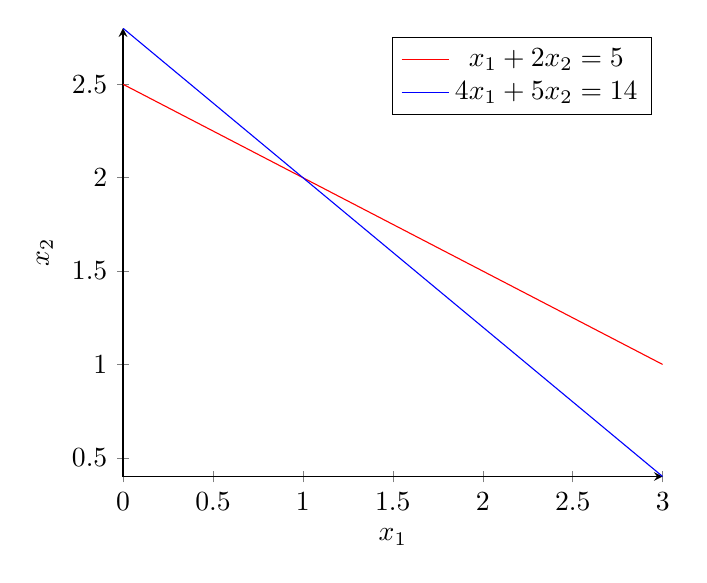
\begin{tikzpicture}
\begin{axis}[
    axis lines = left,
    xlabel = $x_1$,
    ylabel = {$x_2$},
]
%Below the red parabola is defined
\addplot [
    domain=0:3, 
    samples=100, 
    color=red,
]
{2.5-0.5*x};
\addlegendentry{$x_1+2x_2=5$}
%Here the blue parabloa is defined
\addplot [
    domain=0:3, 
    samples=100, 
    color=blue,
    ]
    {-0.8*x+2.8};
\addlegendentry{$4x_1+5x_2=14$}
\end{axis}
\end{tikzpicture}
\paragraph{Column Picture} Focusing on the column of the system of equation, we can denote 
$\begin{bmatrix}
1\\4
\end{bmatrix}$ and $\begin{bmatrix}
2\\5
\end{bmatrix}
$ as vectors in coordinate axis. {Could the linear combinations of these two vectors form the vector}
$\begin{bmatrix}
5\\14
\end{bmatrix}$?  If we denote $x_1$ and $x_2$ as coefficients, it suffices to solve the equation 
$
x_1\begin{bmatrix}
1\\4
\end{bmatrix} + x_2\begin{bmatrix}
2\\5
\end{bmatrix} = \begin{bmatrix}
5\\14
\end{bmatrix}$.

\subsubsection{The solutions of the Linear System of Equations}
The solution to linear system equation could only be \emph{unique}, \emph{infinite}, or \emph{empty}. Let's talk about it case by case in graphic way:
\paragraph{Case 1: unique solution} If two lines intersect at one point, then there is unique solution.
\begin{center}
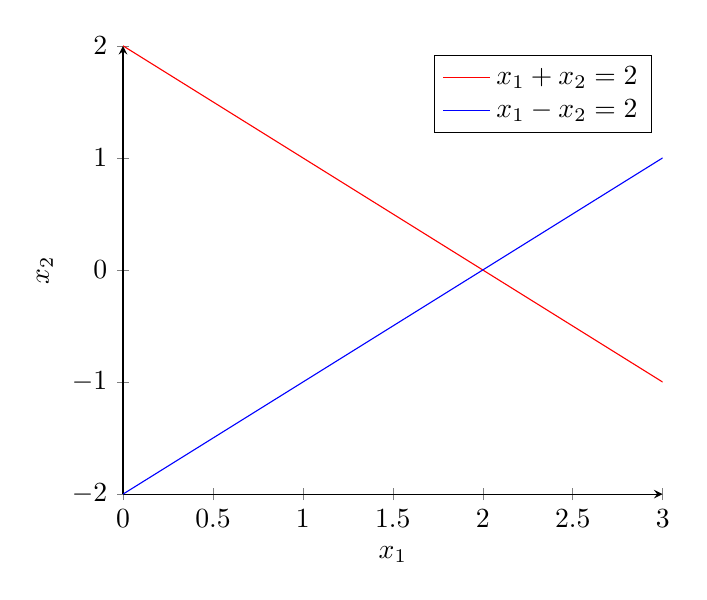
\begin{tikzpicture}
\begin{axis}[
    axis lines = left,
    xlabel = $x_1$,
    ylabel = {$x_2$},
]
%Below the red parabola is defined
\addplot [
    domain=0:3, 
    samples=100, 
    color=red,
]
{2-x};
\addlegendentry{$x_1+x_2=2$}
%Here the blue parabloa is defined
\addplot [
    domain=0:3, 
    samples=100, 
    color=blue,
    ]
    {x-2};
\addlegendentry{$x_1-x_2=2$}
\end{axis}
\end{tikzpicture}
\end{center}
\paragraph{Case2: no solution} If two lines are parallel, then there is no solution.
\begin{center}
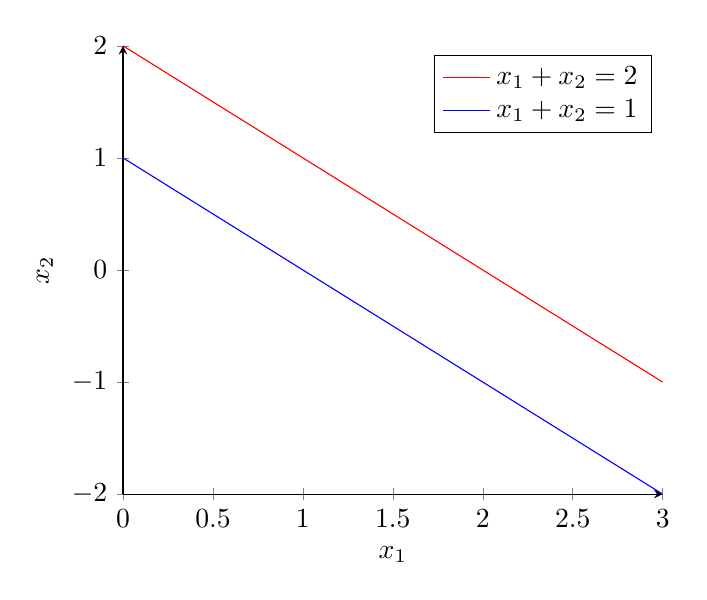
\begin{tikzpicture}
\begin{axis}[
    axis lines = left,
    xlabel = $x_1$,
    ylabel = {$x_2$},
]
%Below the red parabola is defined
\addplot [
    domain=0:3, 
    samples=100, 
    color=red,
]
{2-x};
\addlegendentry{$x_1+x_2=2$}
%Here the blue parabloa is defined
\addplot [
    domain=0:3, 
    samples=100, 
    color=blue,
    ]
    {1-x};
\addlegendentry{$x_1+x_2=1$}
\end{axis}
\end{tikzpicture}
\end{center}
\paragraph{Case 3: infinite number of solutions} If both equations represent the same line, then there are infinite number of solutions.
\begin{center}
\begin{tikzpicture}
\begin{axis}[
    axis lines = left,
    xlabel = $x_1$,
    ylabel = {$x_2$},
]
%Below the red parabola is defined
\addplot [
    domain=0:3, 
    samples=100, 
    color=red,
]
{2-x};
\addlegendentry{$x_1+x_2=2$}
%Here the blue parabloa is defined
\addplot [
    domain=0:3, 
    samples=100, 
    color=blue,
    ]
    {2-x};
\addlegendentry{$-x_1-x_2=-2$}
 
\end{axis}
\end{tikzpicture}
\end{center}
\subsubsection{How to solve $3 \times 3$ Systems?}

\begin{example} \qquad
\\
Let's recall how to solve a $3 \times 3$ system equations as below:

\[
\left \{	\begin{gathered}
2x_1 + x_2 +x_3=5 	\\
4x_1 + (-6)x_2 = -2 \\
-2x_2+7x_2+2x_3 = 9
\end{gathered}	\right.
\]
We can simplify the equation system above into the \emph{Augmented matrix} form:
\[
\left \{	\begin{gathered}
2x_1 + x_2 +x_3=5 	\\
4x_1 + (-6)x_2 = -2 \\
-2x_2+7x_2+2x_3 = 9
\end{gathered}	\right.
\qquad \implies \qquad
\left[
\begin{array}{@{}ccc|c@{}}
2 & 1 & 1 & 5\\
4 & -6 & 0 & -2\\
-2 & 7 & 2 & 9
\end{array}
\right]
\]
%
\[
\xLongrightarrow[\text{Add row 1 to row 3}]{\text{Add $(-2)\times$ row 1 to row 2}}{\quad\quad}
\left[
\begin{array}{@{}ccc|c@{}}
2 & 1 & 1 & 5\\
0 & -8 & -2 & -12\\
0 & 8 & 3 & 14
\end{array}
\right]
\]
\[\xLongrightarrow{\text{Add row 2 to row 3}}{\quad\quad}
\left[
\begin{array}{@{}ccc|c@{}}
2 & 1 & 1 & 5\\
0 & -8 & -2 & -12\\
0 & 0 & 1 & 2
\end{array}
\right]\]
This augmented matrix is the \emph{strictly triangular system}, and it's trial to get the final solution:
\[\implies
\begin{pmatrix}
x_1\\x_2\\x_3
\end{pmatrix}=
\begin{pmatrix}
1\\1\\2
\end{pmatrix}\]
\end{example}

Here we give the definition for strictly triangular system:
\begin{definition}[strictly triangular system]
For the augmented matrix
\[
\left[
\begin{array}{@{}cccc|c@{}}
a_{11} & a_{12} & \dots & a_{1n} &  b_1 \\
a_{21} & a_{22} & \dots & a_{2n} &  b_2 \\
\vdots    & \vdots    & \ddots & \vdots    & \vdots \\
a_{m1} & a_{m2} & \cdots & a_{mn} &   b_n
\end{array}
\right],
\]
if in the $k$th row, the first $(k-1)$th column entries are \textit{all zero} and the $k$th column entries is nonzero, we say the augmented matrix(or corresponding system equation) is of \emph{strictly triangular form}. This kind of matrix(or corresponding system equation) is called \emph{strictly triangular system}.
$(k = 1, . . . , m).$
\end{definition}

\subsubsection{How to solve $n \times n$ System?}
We try to reduce an $n \times n$ System to strictly triangular form. Let's take a special example:
\begin{example}
Given an $n \times n$ System of the form:
\begin{equation}\left[
\begin{array}{@{}cccc|c@{}}
a_{11} & a_{12} & \dots & a_{1n} &  b_1 \\
a_{21} & a_{22} & \dots & a_{2n} &  b_2 \\
\vdots    & \vdots    & \ddots & \vdots    & \vdots \\
a_{n1} & a_{n2} & \cdots & a_{nn} &   b_n
\end{array}\right]\label{eq:n*n_matrix}\end{equation}
Assuming the \emph{diagonal entries} are always \textit{nonzero} during our operation. 
Add row 1 that multiplied by a constant to other $n-1$ row to ensure the first entry of other $n-1$ rows are all \textit{zero}:
\begin{equation}
\implies 
\left[
\begin{array}{@{}cccc|c@{}}
a_{11} & a_{12} & \dots & a_{1n} &  b_1 \\
0 & \x & \dots & \x &  \x \\
\vdots    & \vdots    & \ddots & \vdots    & \vdots \\
0 & \x & \cdots & \x &   \x
\end{array}
\right] \label{eq:n*n_matrix_version1}\end{equation}


Then we proceed this way $n-1$times to obtain:
\begin{equation}
  \left[
    \begin{array}{@{}ccccc|c@{}}
    \x    & \x       & \x    & \x    & \x & \x\\ \cline{1-1}
    \bord & \x       & \x    & \x    & \x & \x\\ \cline{2-2}
          & \bord    & \x    & \x    & \x & \vdots \\ \cline{3-3}
          & \bigzero & \bord & \x    & \x & \vdots \\ \cline{4-4}
          &          &       & \bord & \x & \x \\ \cline{5-5}
  \end{array}\right]\label{eq:n*n_matrix_version2}
\end{equation}

This matrix is the \emph{Row-echelon form}.
And we do the back substitution again to obtain:
\begin{equation}
  \left[
    \begin{array}{@{}ccccc|c@{}}
    \x    &        &     &     &  & \x\\ \cline{1-1}
    \bord & \x       &     &     & \bigzero & \x\\ \cline{2-2}
          & \bord    & \x    &     &  & \vdots \\ \cline{3-3}
          & \bigzero & \bord & \x    &  & \vdots \\ \cline{4-4}
          &          &       & \bord & \x & \x \\ \cline{5-5}
  \end{array}\right]\label{eq:n*n_matrix_version3}
\end{equation}
This matrix is the \emph{Reduced Row-Echelon Form}.
Finally by multiplying every row by a nonzero constant to ensure its \emph{diagnoal entries} are all $1$:
\begin{equation}
  \left[
    \begin{array}{@{}ccccc|c@{}}
    1    &        &     &     &  & \x\\ \cline{1-1}
    \bord & 1       &     &     & \bigzero & \x\\ \cline{2-2}
          & \bord    & \ddots    &     &  & \vdots \\ \cline{3-3}
          & \bigzero & \bord & 1    &  & \vdots \\ \cline{4-4}
          &          &       & \bord & 1 & \x \\ \cline{5-5}
  \end{array}\right]\label{eq:n*n_matrix_version4}
\end{equation}
\end{example}

Then let's analysis the complexity of solving such a $n\times n$ system.
\subsection{Complexity Analysis}
\subsubsection{Step1: Reduction from matrix (\ref{eq:n*n_matrix}) to matrix (\ref{eq:n*n_matrix_version1})}
\begin{proposition}
The time complexity for Augmented matrix reduction using back-substitution algorithm is $\mathcal{O}(n^3)$.
\end{proposition}

\begin{proof}
The estimation for the time complexity requires us to estimate how many steps of \emph{multiplication} we need. (The time for addition is so small that can be ignored).
\begin{itemize}
\item
Reducing matrix (\ref{eq:n*n_matrix}) to matrix (\ref{eq:n*n_matrix_version1}) we need to do $n(n-1)$times multiplications.

This is because for each row (except first row) we have known the first entry is zero, while the remaining $(n-1)$ entries in each row should be computed by multiplying first row's entries and then add it to the row.
\item
Then it suffices to deal with the inner $(n-1)\times (n-1)$ matrix, which requires the $(n-1)\times (n-2)$ times multiplication.
\item
The back substitution for matrix (\ref{eq:n*n_matrix}) requires $n$ times reduction.
\end{itemize}
Hence the total multiplication times for back substitution for matrix (\ref{eq:n*n_matrix}) is
\begin{equation*}
\begin{split}
\sum_{i=1}^n i(i-1)
	&= \sum_{i=1}^n (i^2-i)  \\
 		&=\sum_{i=1}^n i^2 - \sum_{i=1}^n i \\
		&=\frac{n(n+1)(2n+1)}{6} - \frac{n(n+1)}{2} \\
		&=\frac{n^3-2n}{3} \sim \frac{n^3}{3} =O(n^3)
\end{split}
\end{equation*}
\end{proof}
But we can always develop more advanced algorithm that have smaller time complexity.

\subsubsection{Step2: Reduction from triangular system to diagonal system}

In order to reducing matrix (\ref{eq:n*n_matrix_version2}) to matrix (\ref{eq:n*n_matrix_version3}) we need to do back-substitution again. The matrix (\ref{eq:n*n_matrix_version3}) is diagonal system. Obviously, for this process the total multiplication times is given by
\[
1+2+\cdots+n-1 = \frac{n(n-1)}{2} \sim O(n^2)
\]
\subsubsection{Step3: Get final solution}

In the final step, we want to reduce matrix (\ref{eq:n*n_matrix_version3}) to matrix (\ref{eq:n*n_matrix_version4}), the only thing we need to do is to do one multiplication for each row to let the diagonal entries be $1$. Hence the total multiplication times for this process is given by
\[
\underbrace{1+1+\dots+1}_{\text{totally $n$ terms}} = O(n)
\]
\subsection{Brief Summary}
The reduction of $n\times n$ matrix requires three kinds of Row operations:
\begin{itemize}
\item \emph{Addition and Multiplication}.

Add to a row by a constant multiple of another row.

\item \emph{Multiplication}

Multiply a row by a nonzero constant.
\item \emph{Interchange}

Interchange two rows
\end{itemize}


\begin{enumerate}
\item
agds
\end{enumerate}•

\section{Thursday}\index{week5_Thursday_lecture}
\subsection{Orthogonality and Projection}
Two vectors are orthogonal if their inner product is zero:
\[
\bm u\perp\bm v
\Longleftrightarrow
\inp{\bm u}{\bm v}=0\qquad\text{(if $\bm u,\bm v\in\mathbb{R}^{n}$, then $\bm u\trans\bm v=0$.)}
\]
And orthogonality among vectors has an important property:
\begin{proposition}\qquad\\
If \emph{nonzero} vectors $v_1,\dots,v_k$ are mutually orthogonal (mutulally means $v_i\perp v_j$ for any $i\ne j$), then $\{v_1,\dots,v_k\}$ must be ind.
\end{proposition}
\begin{proof}
We only need to show that 
\[
\text{if }\alpha_1v_1+\dots+\alpha_kv_k=\bm 0,\qquad
\text{then }
\alpha_i=0\text{ for any $i\in\{1,2,\dots,k\}$.}
\]
\begin{itemize}
\item
We do inner product to show $\alpha_1$ must be zero:
\[
\begin{aligned}
\inp{v_1}{\alpha_1v_1+\dots+\alpha_kv_k}
&=\inp{v_1}{\bm 0}=0\\
&=\alpha_1\inp{v_1}{v_1}+\alpha_2\inp{v_1}{v_2}+\dots+\alpha_k\inp{v_1}{v_k}\\
&=\alpha_1\inp{v_1}{v_1}=\alpha_1\|v_1\|_2^2\\
&=0
\end{aligned}
\]
Since $v_1\ne \bm 0$, we have $\alpha_1=0$.
\item
Similarly, we have $\alpha_i=0$ for $i=1,\dots,k$.
\end{itemize}
\end{proof}
Now we can also talk about orthogonality among spaces:
\enlargethispage{2cm}
\begin{definition}[subspace orthogonality]
Two subspaces $\bm U$ and $\bm V$ of a vector space are \emph{orthogonal} if every vector $\bm u$ in $\bm U$ is \textit{perpendicular} to every vector $\bm v$ in $\bm V$:
\[
\text{\emph{Orthogonal subspaces}}\qquad
\bm u\perp\bm v\quad\forall\bm u\in\bm U,\bm v\in\bm V.
\]
\end{definition}
\begin{example}
Two walls look \textit{perpendicular} but they are not orthogonal subspaces! The meeting line is in both $\bm U$ and $\bm V$-and this line is not perpendicular to itself. Two planes (dimensions $2$ and $2$ in $\mathbb{R}^{3}$) cannot be orthogonal subspaces.\\
\begin{figure}[H]
\centering
\includegraphics{week5/orthogonality}
\caption{Orthogonality is impossible when $\dim\bm U+\dim\bm V>\dim(\bm U\cup\bm V)$}
\end{figure}
\end{example}
\begin{remark}
When a vector is in two orthogonal subspaces, it \textit{must} be zero. It is \emph{perpendicular} to
itself. 
\\The reason is clear: this vector $\bm u\in\bm U$ and $\bm u\in\bm V$, so $\inp{\bm u}{\bm u}=0$. It has to be zero vector.
\end{remark}
If two subspaces are perpendicular, their basis must be ind.
\begin{theorem}
Assume $\{u_1,\dots,u_k\}$ is the basis for $\bm U$, $\{v_1,\dots,v_l\}$ is the basis for $\bm V.$ If $\bm U\perp\bm V$ ($u_i\perp v_j$ for $\forall i,j$), then $u_1,u_2,\dots,u_k,v_1,v_2,\dots,v_l$ must be ind.
\end{theorem}
\begin{proof}
Suppose there exists $\{\alpha_1,\dots,\alpha_k\}$ and $\{\beta_1,\dots,\beta_l\}$ such that
\[
\alpha_1u_1+\dots+\alpha_ku_k+\beta_1v_1+\dots+\beta_lv_l=\bm 0
\]
then equibalently,
\[
\alpha_1u_1+\dots+\alpha_ku_k=-(\beta_1v_1+\dots+\beta_lv_l)
\]
Then we set $\bm w=\alpha_1u_1+\dots+\alpha_ku_k$, obviously, $\bm w\in\bm U$ and $\bm w\in\bm V$.\\ Hence it must be zero (This is due to remark above). Thus we have
\begin{gather*}
\alpha_1u_1+\dots+\alpha_ku_k=\bm 0\\
\beta_1v_1+\dots+\beta_lv_l=\bm 0.
\end{gather*}
Due to the independence, we have $\alpha_i=0$ and $\beta_j=0$ for $\forall i,j$. 
\end{proof}
\begin{corollary}
If $\{u_1,u_2,\dots,u_k,v_1,v_2,\dots,v_l\}\in\bm W$, then $\dim(\bm W)\ge\dim(\bm U)+\dim(\bm V)$.\\ Note that $\bm U\cup\bm V\subset\bm W$.
\end{corollary}
For subspaces $\bm U$ and $\bm V\in\mathbb{R}^{n}$, if $\mathbb{R}^{n}=\bm U\cup\bm V$, and moreover, $n=\dim(\bm U)+\dim(\bm V)$, then we say $\bm V$ is the \emph{orthogonal complement} of $\bm U$.
\begin{definition}[orthogonal complement]
For subspaces $\bm U$ and $\bm V\in\mathbb{R}^{n}$, if $\dim(\bm U)+\dim(\bm V)=n$ and $\bm U\perp\bm V$, then we say $\bm V$ is the \emph{orthogonal complement} of $\bm U$. And we denote $\bm V$ as $\bm U^{\perp}$.\\
Moreover, $\bm V=\bm U^{\perp}\Longleftrightarrow\bm V^{\perp}=\bm U$.
\end{definition}
\begin{example}
Suppose $\bm U\cup\bm V=\mathbb{R}^{3}$, $\bm U=\Span\{\bm e_1,\bm e_2\}$. If $\bm V$ is the orthogonal complement of $\bm U$, then $\bm V=\Span\{\bm e_3\}$. \\Moreover, $\bm U$ could also be expressed as $\Span\left\{\begin{pmatrix}
1\\1\\0
\end{pmatrix},\begin{pmatrix}
0\\1\\0
\end{pmatrix}\right\}$.
\end{example}
\emph{Example:}\\
Next let's show the nullspace is the orthogonal complement of the row space. (In $\mathbb{R}^{n}$).
Suppose $\bm A$ is a $m\times n$ matrix.
\begin{itemize}
\item
Firstly, we show $\dim(N(\bm A))+\dim(C(\bm A\trans))=\dim(N(\bm A)\cup C(\bm A\trans))=\dim(\mathbb{R}^{n})=n$:\\
We know $\dim(N(\bm A))=n-r$, where $r=\rank(\bm A)$. And $r=C(\bm A\trans))$.\\ Hence $\dim(N(\bm A))+\dim(C(\bm A\trans))=n$.
\item
Then we show $N(\bm A)\perp C(\bm A\trans)$:\\
For any $x\in N(\bm A)$, if we set $\bm A=\begin{bmatrix}
a_1\\a_2\\\vdots\\a_m
\end{bmatrix}$, then we obtain:
\[
\bm{Ax}=\begin{bmatrix}
a_1\\a_2\\\vdots\\a_m
\end{bmatrix}\begin{bmatrix}
\bm x
\end{bmatrix}=\begin{bmatrix}
0\\0\\\vdots\\0
\end{bmatrix}
\]
Hence \textit{every row has a zero product with} $x$. In other words, $\inp{a_i}{x}=0$ for $\forall i\in\{1,2,\dots,m\}$.\\
Hence for any $y=\sum_{i=1}^m\alpha_ia_i\in C(\bm A\trans)$, we obtain:
\[
\begin{aligned}
\inp{x}{y}&=\inp{y}{x}=\inp{\sum_{i=1}^m\alpha_ia_i}{x}\\
&=\sum_{i=1}^{m}\alpha_i\inp{a_i}{x}=0.
\end{aligned}
\]
Hence $x\perp y$ for $\forall x\in N(\bm A)$ and $y\in C(\bm A\trans)$.\\
\end{itemize}
Hence $N(\bm A)^{\perp}=C(\bm A\trans)$.\\
If we applying this equation to $\bm A\trans$, then we have $N(\bm A\trans)^{\perp}=C(\bm A)$. 
\enlargethispage{1cm}
\begin{theorem}[Fundamental theorem for linear alegbra, part 2]\qquad\\
\emph{$N(\bm A)$ is the orthogonal complement of the row space $C(\bm A\trans)$ (in $\mathbb{R}^{n}$).}\\
\emph{$N(\bm A\trans)$ is the orthogonal complement of the row space $C(\bm A)$ (in $\mathbb{R}^{m}$).}
\end{theorem}
\newpage
\begin{corollary}
$\bm{Ax}=\bm b$ is solvable if and only if $\bm y\trans\bm A=\bm 0$ implies $\bm y\trans\bm b$=0.
\end{corollary}
\begin{proof}\qquad\\
$\bm{Ax}=\bm b$ is solvable.
$\Longleftrightarrow$
$\bm b\in C(\bm A)$.
$\Longleftrightarrow$
$\bm b\in N(\bm A\trans)^{\perp}$\\
$\Longleftrightarrow$
$\bm y\trans\bm b=0$ for $\forall y\in N(\bm A\trans)$
$\Longleftrightarrow$
$\bm y\trans\bm A=\bm 0$ implies $\bm y\trans\bm b$=0.
\end{proof}
The Inverse Negative Propositions is more important:
\begin{corollary}
$\bm{Ax}=\bm b$ has no solution if and  and only if $\exists \bm y$ s.t. $\bm y\trans\bm A=0$ and $\bm y\trans\bm b\ne 0$.
\end{corollary}
\begin{remark}
\begin{theorem}\label{theorem_12.3}
$\bm{Ax}\ge\bm b$ has no solution if and only if $\exists \bm y\ge\bm 0$ such that $\bm y\trans\bm A=\bm 0$ and $\bm y\trans\bm b\ge \bm 0$.
\end{theorem}
$\bm y\trans\bm A=0$ requires exists one linear combination of the row space to be zero.
\begin{proof}[Necessity case.]
Suppose $\exists \bm y\ge\bm 0$ such that $\bm y\trans\bm A=\bm 0$ and $\bm y\trans\bm b\ge \bm 0$. And we assume there exists $x^{*}$ such that $\bm Ax^{*}\ge\bm b$. By postmultiplying $\bm y\trans$ we have 
\[\bm y\trans\bm Ax^{*}\ge\bm y\trans\bm b>\bm 0
\implies 
\bm 0>\bm 0.
\]
which is a contradiction!
\end{proof}
The complete proof for this theorem is not required in this course.
\end{remark}
\begin{example}
Given the system 
\begin{equation}
\begin{aligned}
x_1+x_2&\ge1\\
-x_1&\ge-1\\
-x_2&\ge2
\end{aligned}
\end{equation}
Eq(1)$\x$1+Eq(2)$\x$1+Eq(3)$\x$1 gives
\[
0\ge 2
\]
which is a contradiction!\\
So the key idea of theorem (\ref{theorem_12.3}) is to construct a linear combination of row space to let it become zero. Then if the right hand is larger than zero, then this system has no solution.
\end{example}
\begin{remark}
\begin{corollary}
If $\bm A=\bm A\trans$, then $N(\bm A\trans)^{\perp}=C(A)=C(\bm A\trans)=N(\bm A)$.
\end{corollary}
\begin{corollary}\label{corollary_12.5}
The system $\bm{Ax}=\bm b$ may not have a solution, but $\bm A\trans\bm A\bm x=\bm A\trans\bm b$ always have at least one solution for $\forall\bm b$.
\end{corollary}
\begin{proof}
Since $\bm A\trans\bm A$ is symmetric, we have $C(\bm A\trans\bm A)=C(\bm A\bm A\trans)$. You can check by yourself that $C(\bm A\bm A\trans)=C(\bm A\trans)$.
Hence $C(\bm A\trans\bm A)=C(\bm A\trans)$.\\
For any vector $\bm b$ we have $\bm A\trans\bm b\in C(\bm A\trans)\implies\bm A\trans\bm b\in C(\bm A\trans\bm A)$, which means there exists a linear combination of the columns of $\bm A\trans\bm A$ that equals to $\bm b$.\\
Equivalently, there exists a solution to $\bm A\trans\bm A\bm x=\bm A\trans\bm b$.
\end{proof}
\begin{corollary}\label{corollary_12.6}
$\bm A\trans\bm A$ is invertible if and only if columns of $\bm A$ are ind.
\end{corollary}
\begin{proof}
We have shown that $C(\bm A\trans\bm A)=C(\bm A\trans)$.\\ Hence $C(\bm A\trans\bm A)^{\perp}=C(\bm A\trans)^{\perp}\implies N(\bm A\trans\bm A)=N(\bm A)$.\\
$\bm A$ has ind. columns
$\Longleftrightarrow$
$N(\bm A)=\{\bm 0\}$
$\Longleftrightarrow$
$N(\bm A\trans\bm A)=\{\bm 0\}$
$\Longleftrightarrow$
$\bm A\trans\bm A$ is invertible.
\end{proof}
\end{remark}
\subsection{Least Squares Approximations}
$\bm{Ax}=\bm b$ often has no solution, if so, what should we do?\\
We cannot always get the error $\bm e=\bm b-\bm{Ax}$ down to zero, so we want to use least square method to minimize the error. In other words, our goal is to
\[
\min_{\bm x}\bm e^2=\min_{\bm x}\|\bm{Ax}-\bm b\|^2=\sum_{i=1}^{m}(a_i\trans\bm x-b_i)^2
\]
where $\bm A=\begin{bmatrix}
a_1\\a_2\\\vdots\\a_m
\end{bmatrix}$ and $\bm b=\begin{bmatrix}
b_1\\b_2\\\vdots\\b_m
\end{bmatrix}$.\\
The minimizer $\bm x$ is called \emph{linear least squares solution}.
\subsubsection{Matrix Calculus}
Firstly, you should know some basic calculus knowledge for matrix:
\begin{itemize}
\item
$\frac{\partial(f\trans g)}{\partial x}=\frac{\partial f(x)}{\partial x}g(x)+\frac{\partial g(x)}{\partial x}f(x)$
\end{itemize}
Example:
\begin{itemize}
\item
$\frac{\partial(a\trans \bm x)}{\partial \bm x}=a$
\item
$\frac{\partial(a\trans \bm A\bm x)}{\partial \bm x}=\frac{\partial((\bm A\trans a)\trans\bm x)}{\partial \bm x}=\bm A\trans a$
\item
$\frac{\partial(\bm A\bm x)}{\partial \bm x}=\bm A\trans$
\item
$\frac{\partial(\bm x\trans\bm A\bm x)}{\partial \bm x}=\bm A\bm x+\bm A\trans\bm x$
\end{itemize}
Thus, in order to minimize $\|\bm{Ax}-\bm b\|^2=(\bm{Ax}-\bm b)\trans(\bm{Ax}-\bm b)$, we only need to let its \emph{partial derivative} with respect to $\bm x$ to be \emph{zero.} (Since its second derivative is non-negative, we will talk about it in detail in other courses.) Hence we have
\[\begin{aligned}
\frac{\partial (\bm{Ax}-\bm b)\trans(\bm{Ax}-\bm b)}{\partial \bm x}&=\frac{\partial(\bm{Ax}-\bm b)}{\partial \bm x}(\bm{Ax}-\bm b)+\frac{\partial(\bm{Ax}-\bm b)}{\partial \bm x}(\bm{Ax}-\bm b)=2\frac{\partial(\bm{Ax}-\bm b)}{\partial \bm x}(\bm{Ax}-\bm b)\\
&=2(\frac{\partial(\bm A\bm x)}{\partial \bm x}-\frac{\partial(\bm b)}{\partial \bm x})(\bm{Ax}-\bm b)\\
&=2\bm A\trans(\bm{Ax}-\bm b)=\bm 0.
\end{aligned}
\]
Or equivalently, 
\[
\bm A\trans\bm{Ax}=\bm A\trans\bm b.
\]
According to corollary (\ref{corollary_12.5}), this equation always exists a solution. And this equation is called \emph{normal equation}.
\begin{theorem}\label{theorem_12.4}
The partial derivatives of $\|\bm{Ax}-\bm b\|^2$ are \emph{zero} when $\bm A\trans\bm{Ax}=\bm A\trans\bm b.$
\end{theorem}
\subsubsection{Fit a stright line}
Given a collection of data $(\bm x_i,y_i)$ for $i=1,\dots,m$, we can fit the model parameters:
\[
\left\{
\begin{aligned}
y_1&=a_0+a_1x_{1,1}+a_2x_{1,2}+\dots+a_nx_{1,n}+\varepsilon_1\\
y_2&=a_0+a_1x_{2,1}+a_2x_{2,2}+\dots+a_nx_{2,n}+\varepsilon_2\\
\vdots\\
y_m&=a_0+a_1x_{m,1}+a_2x_{m,2}+\dots+a_nx_{m,n}+\varepsilon_m
\end{aligned}
\right.
\]
Our fit line is 
\[
\hat y=a_0+a_1x_1+a_2x_2+\dots+a_nx_n
\]
In \textit{compact matrix form}, we have
\[
\begin{bmatrix}
y_1\\y_2\\\vdots\\y_n
\end{bmatrix}
=\begin{bmatrix}
1&x_{1,1}&x_{1,2}&\dots&x_{1,n}\\
1&x_{2,1}&x_{2,2}&\dots&x_{2,n}\\
\vdots&\vdots&&&\\
1&x_{m,1}&x_{m,2}&\dots&x_{m,n}\\
\end{bmatrix}\begin{bmatrix}
a_0\\a_1\\a_2\\\vdots\\a_{n}
\end{bmatrix}+\begin{bmatrix}
\varepsilon_1\\\varepsilon_2\\\vdots\\\varepsilon_m
\end{bmatrix}
\]
Or equivalently, we have 
\[
\bm y=\bm{Ax}+\bm \varepsilon
\]
where $\bm A =\begin{bmatrix}
1&x_{1,1}&x_{1,2}&\dots&x_{1,n}\\
1&x_{2,1}&x_{2,2}&\dots&x_{2,n}\\
\vdots&\vdots&&&\\
1&x_{m,1}&x_{m,2}&\dots&x_{m,n}\\
\end{bmatrix}_{m\times (n+1)}$, $\bm x=\begin{bmatrix}
a_0\\a_1\\a_2\\\vdots\\a_{n}
\end{bmatrix}_{(n+1)\times 1}$, $\bm \varepsilon=\begin{bmatrix}
\varepsilon_1\\\varepsilon_2\\\vdots\\\varepsilon_m
\end{bmatrix}_{m\times 1}$.\\
Our goal is to minimize $\|\hat{\bm y}-\bm y\|^2=\|\bm{Ax}-\bm y\|^2$. Then by theorem (\ref{theorem_12.4}), we only need to sovle $\bm A\trans\bm A\bm x=\bm A\trans\bm y$.
\subsection{Projections}
In corollary (\ref{corollary_12.6}), we know that if $\bm A$ has ind. columns, then $\bm A\trans\bm A$ is invertible. On this condition, the normal equation $\bm A\trans\bm A\bm x=\bm A\trans\bm b$ has unique solution $\bm x^{*}=(\bm A\trans\bm A)^{-1}\bm A\trans\bm b$.\\
Thus the error $\bm b-\bm A\bm x^{*}$ is minimum. And $\bm A\bm x^{*}=\bm A(\bm A\trans\bm A)^{-1}\bm A\trans\bm b$ \emph{approximately} equals to $\bm b$. \\
\begin{itemize}
\item
If $\bm b$ and $\bm{A}\bm x^{*}$ are exactly in the same space, then $\bm{A}\bm x^{*}=\bm b$.
\item
Otherwise, just as the Figure (\ref{figure_12.2}) shown, $\bm A\bm x^{*}$ is the projection of $\bm b$ to subspace $C(\bm A)$.
\end{itemize}
\begin{figure}[H]\centering
\includegraphics{week5/projection}
\caption{The projection of $\bm b$ onto a subspace $C(\bm A)$.}\label{figure_12.2}\end{figure}
\begin{definition}[Projection]
The projection of $\bm b$ onto the subspace $C(\bm A)$ is denoted as $\Proj_{C(\bm A)}(\bm b)$.
\end{definition}
\begin{definition}[Projection matrix]
Given $\bm A\bm x^{*}=\bm A(\bm A\trans\bm A)^{-1}\bm A\trans\bm b=\Proj_{C(\bm A)}(\bm b)$. Since $[\bm A(\bm A\trans\bm A)^{-1}\bm A\trans]\bm b$ is the projection of $\bm b$, we call $\bm P=\bm A(\bm A\trans\bm A)^{-1}\bm A\trans$ as \emph{projection matrix}.
\end{definition}
\begin{definition}[Idempotent]
Let $\bm A$ be a \emph{square} matrix that satisfies $\bm A=\bm A\bm A$, then $\bm A$ is called a \emph{idempotent} matrix.
\end{definition}
Let's show the projection matrix is \textit{idempotent}:\\
\[
\begin{aligned}
\bm P^{2}&=\bm A(\bm A\trans\bm A)^{-1}\bm A\trans\bm A(\bm A\trans\bm A)^{-1}\bm A\trans\\
&=\bm A(\bm A\trans\bm A)^{-1}(\bm A\trans\bm A)(\bm A\trans\bm A)^{-1}\bm A\trans\\
&=\bm A(\bm A\trans\bm A)^{-1}\bm A\trans=\bm P.
\end{aligned}
\]
\subsubsection{Observations}
\begin{itemize}
\item
If $\bm b\in C(\bm A)$, then $\exists \bm x$ s.t. $\bm{Ax}=\bm b$. Moreover, the projection of $\bm b$ is exactly $\bm b$:
\[
\begin{aligned}
\bm{Pb}&=\bm A(\bm A\trans\bm A)^{-1}\bm A\trans(\bm b)\\
&=\bm A(\bm A\trans\bm A)^{-1}\bm A\trans(\bm{Ax})\\
&=\bm A(\bm A\trans\bm A)^{-1}(\bm A\trans\bm A)\bm x\\
&=\bm{Ax}=\bm b.
\end{aligned}
\]
\item
Assume $\bm A$ has only one column, say, $\bm a$. Then we have
\[\begin{aligned}
\bm x^{*}&=(\bm A\trans\bm A)^{-1}\bm A\trans\bm b=\frac{\bm a\trans\bm b}{\bm a\trans\bm a}\\
\bm A\bm x^{*}&=\bm{Pb}=\bm A(\bm A\trans\bm A)^{-1}\bm A\trans(\bm b)=\frac{\bm a\trans\bm b}{\bm a\trans\bm a}\times\bm a=\frac{\bm a\trans\bm b}{\|\bm a\|^2}\times\bm a
\end{aligned}
\]
More interestingly, 
\[\frac{\bm a\trans\bm b}{\|\bm a\|^2}\times\bm a=\frac{\|\bm a\|\|\bm b\|\cos\theta}{\|\bm a\|^2}\times\bm a=\|\bm b\|\cos\theta\times\frac{\bm a}{\|\bm a\|}\]
which is the projection of $\bm b$ onto a line $\bm a$. (Shown in figure below.)
\begin{figure}[H]
\centering\includegraphics[width=10cm]{week5/projection_line}
\caption{The projection of $\bm b$ onto a line $\bm a$.}
\end{figure}
More generally, we can write the projection of $\bm b$ as:
\[
\Proj_{\bm a}(\bm b)=\frac{\inp{\bm a}{\bm b}}{\inp{\bm a}{\bm a}}\bm a
\]
Look at the figure above! The error is $\bm b-\Proj_{\bm a}(\bm b)$, which is obviously perpendicular to $\bm a$. And $\bm b-\Proj_{\bm a}(\bm b)\in\Span\{\bm a,\bm b\}$.\\
If we define $\bm b'=\bm b-\Proj_{\bm a}(\bm b)$, then it's easy to check $\Span\{\bm a,\bm b'\}=\Span\{\bm a,\bm b\}$ and $\bm a\perp\bm b'$. Hence we convert a basis to another basis such that the elements are orthogonal to each other. We will discuss it in detail in next lecture. 
\end{itemize}









\chapterimage{M31_hallas}% Chapter heading image

%\chapter{Week5}

\section{Friday}\index{week5_Friday_lecture}
This lecture has two goals. The first is to see \emph{how orthogonality makes it easy to find projection matrix $\bm P$ and the projection $\Proj_{C(\bm A)}\bm b$}. \textit{Orthogonality makes the product $\bm A\trans\bm A$ a diagonal matrix}. The second goal is to \emph{show how to construct orthogonal vectors}. For matrix $\bm A=\begin{bmatrix}
a_1&a_2&\dots&a_n
\end{bmatrix}$, the columns may not be orthogonal. Then we convert $a_1,\dots,a_n$ to orthogonal vectors, which will be the columns of a new matrix $\bm Q$.
\subsection{Orthonormal basis}
The vectors $\bm q_1,\dots,\bm q_n$ are \emph{orthogonal} when their inner product $\inp{\bm q_i}{\bm q_j}$ are zero. ($i\ne j$.) With one more step--just divide each vector by its length, then the vectors become \emph{orthogonal unit vectors}. Their lengths are all 1. Then its basis is called \emph{orthonormal}.
\begin{definition}[orthonormal]
The vectors $\bm q_1,\dots,\bm q_n$ are \emph{orthonormal} if
\[
\inp{\bm q_i}{\bm q_j}=\begin{cases}
0&\text{when $i\ne j$}\qquad\text{(\emph{orthogonal} vectors)},\\
1&\text{when $i=j$}\qquad\text{(\emph{unit} vectors: $\|\bm q_i\|=1$)}.
\end{cases}
\]
Moreover, if $\bm q_1,\dots,\bm q_n$ are \emph{orthonormal}, then the basis $\{\bm q_1,\dots,q_n\}$ is called \emph{orthonormal basis}.
\end{definition}
\begin{example}
Unit vectors $\bm e_1=\begin{pmatrix}
1\\0\\\vdots\\0
\end{pmatrix},\bm e_2=\begin{pmatrix}
0\\1\\\vdots\\0
\end{pmatrix},\dots,\bm e_n=\begin{pmatrix}
0\\0\\\vdots\\1
\end{pmatrix}$ is an \textit{orthonormal basis} for $\mathbb{R}^{n}$.
\end{example}
If we want to express vector $\bm b$ as a linear combination of arbitrary basis $\{\bm q_1,\bm q_2,\dots,\bm q_n\}$, what should you do?\\
\textit{Answer:} To solve the system $\bm{Ax}=\bm b$, where $\bm A=\begin{bmatrix}
\bm q_1&\bm q_2&\dots&\bm q_n
\end{bmatrix}$.\\
What if $\{\bm q_1,\bm q_2,\dots,\bm q_n\}$ form an \emph{orthogonal} basis? How to find solution $\bm x$ s.t. 
\[
\bm b=x_1\bm q_1+x_2\bm q_2+\dots+x_n\bm q_n?
\]
\textit{Answer}: We just do the inner product of each $\bm q_i$ with $\bm b$ to get the coefficient $x_i$:
\[
\begin{aligned}
\inp{\bm q_i}{\bm b}&=x_1\inp{\bm q_i}{\bm q_1}+x_2\inp{\bm q_i}{\bm q_2}+\dots+x_n\inp{\bm q_i}{\bm q_n}\\
&=x_i\inp{\bm q_i}{\bm q_i}=x_i
\end{aligned}
\]
Since $x_i=\inp{\bm q_i}{\bm b}$, we could express $\bm b$ as:
\[
\bm b=\sum_{i=1}^{n}\inp{\bm q_i}{\bm b}\bm q_i.
\]
In this case, since $\{\bm q_1,\bm q_2,\dots,\bm q_n\}$ forms a basis, the columns of $\bm A$ must be ind. Hence $\bm A$ is invertible, then we get the solution to $\bm{Ax}=\bm b$:
\begin{equation}
\bm x=\bm A^{-1}\bm b.
\end{equation}
\begin{definition}[matrix with orthonormal columns]\qquad\\
Define $\bm Q=\begin{bmatrix}
q_1&q_2&\dots&q_n
\end{bmatrix}$. If vectors $\bm q_1,\dots,\bm q_n$ are \emph{orthonormal}, then we say $\bm Q$ is a matrix with \emph{orthonormal} columns.
\begin{remark}
Note that a matrix with \emph{orthonormal} columns is often denoted as $\bm Q$.
\end{remark}
\end{definition}
Such matrix \emph{is easy to work with} because we have:
\begin{equation}\label{eq:easy_to_work}
\bm Q\trans\bm Q=\begin{pmatrix}
\bm q_1\trans\\\bm q_2\trans\\\dots\\\bm q_n\trans
\end{pmatrix}\begin{pmatrix}
\bm q_1&\bm q_2&\dots&\bm q_n
\end{pmatrix}=\begin{pmatrix}
\bm q_1\trans\bm q_1&&\\
&\ddots&\\
&&\bm q_n\trans\bm q_n
\end{pmatrix}=\bm I.
\end{equation}
\begin{remark}
Note that a matrix with orthonormal columns $\bm Q$ is \textit{not required to be square}! Moreover, $\{\bm q_1,\dots,\bm q_n\}$ in $\bm Q$ is \textit{not required to form a basis}.
\end{remark}
\begin{definition}[orthogonal matrix]
An \emph{square} that is a \textit{matrix with orthonormal columns} is called \emph{othogonal matrix}.
\end{definition}
\begin{example}\qquad\\
If $\bm Q$ is a orthogonal matrix, while $\bm{\hat\bm Q}$ is a matrix with orthonormal columns that is \emph{not square}. Do the products $\bm Q\bm Q\trans$ and $\bm{\hat Q}\bm{\hat Q\trans}$ always be \textit{identity matrix}?\\
\textit{Answer}:
\begin{itemize}
\item
$\bm Q\bm Q\trans$ is always \textit{identity matrix}. According to equation (\ref{eq:easy_to_work}), we have $\bm Q\trans\bm Q=\bm I$.\\ Hence $\bm Q\trans$ is the left inverse of square matrix $\bm Q$.\\ Hence $\bm Q^{-1}=\bm Q\trans\implies\bm Q\bm Q\trans=\bm Q\bm Q^{-1}=\bm I$.\\
Moreover, solving $\bm{Qx}=\bm b$ is equivalent to $\bm x=\bm Q^{-1}\bm b=\bm Q\trans\bm b$, which is \textit{exactly} 
\[
\bm x=\begin{bmatrix}
\inp{\bm q_1}{\bm b}\\\inp{\bm q_2}{\bm b}\\\vdots\\\inp{\bm q_n}{\bm b}
\end{bmatrix}.
\]
\item
But the product $\bm \hat Q\bm \hat Q\trans$ will never be identity matrix. Assume $\bm \hat Q$ is a $m\times n$ matrix. ($m\ne n$.) Then it's easy to verify that $\rank(\bm \hat Q\bm \hat Q\trans)=\rank(\bm\hat Q)$.\\ Since $\bm\hat Q$ has orthonormal columns, the columns of $\bm\hat Q$ are ind. Hence $\rank(\bm\hat Q)=n$.\\ But $\rank(\bm \hat Q\bm \hat Q\trans)=\rank(\bm\hat Q)=n\ne m=\rank(\bm I_{m})$.\\
Moreover, if $\bm\hat Q$ has only one column $\bm\hat q$, then $\bm \hat Q\bm \hat Q\trans=\bm\hat q\bm\hat q\trans=\rank(1)\ne \bm I_{m}$.
\end{itemize}
\end{example}
\begin{proposition}\quad\\
If $\bm Q$ has orthonormal columns, then it \textit{leaves lengths unchanged}, in other words,
\[
\text{\emph{Same length}}\qquad\qquad
\|\bm{Qx}\|=\|\bm x\|\quad\text{for every vector $\bm x$.}
\]
Also, $\bm Q$ preserves inner products for vectors:
\[
\inp{\bm{Qx}}{\bm{Qy}}=\inp{\bm x}{\bm y}\quad\text{for every vectors $\bm x$ and $\bm y$.}
\]
\end{proposition}
\begin{proof}[Proofoutline.]
$\|\bm{Qx}\|^2=\|\bm x\|^2$ because
\[\begin{aligned}
\inp{\bm{Qx}}{\bm{Qx}}&=\bm x\trans\bm Q\trans\bm Q\bm x=\bm x\trans(\bm Q\trans\bm Q)\bm x\\
&=\bm x\trans\bm I\bm x=\bm x\trans\bm x
\end{aligned}
\]
Hence we have $\|\bm{Qx}\|=\|\bm x\|$. Just using $\bm Q\trans\bm Q=\bm I$, we can derive $\inp{\bm{Qx}}{\bm{Qy}}=\inp{\bm x}{\bm y}$.
\end{proof}
Orthogonal matrices are excellent for computations, since numbers can never grow too large when lengths of vectors are fixed.\\
In particular, if $\bm Q\in\mathbb{R}^{m\times n}$ has orthonormal columns, the least square problem is easy:\\
Although $\bm{Qx}=\bm b$ may not have a solution, but the normal equation
\[
\bm Q\trans\bm Q\bm \hat x=\bm Q\trans\bm b
\]
must have a unique solution $\bm\hat x=\bm Q\trans\bm b$. Why? Since $\bm Q\trans\bm Q=\bm I$, we derive $\bm\hat x=\bm Q\trans\bm Q\bm \hat x=\bm Q\trans\bm b$.\\
\emph{\textit{\Large Summary:}}\\
Hence the \emph{least squares solution} to $\bm{Qx}=\bm b$ is $\bm\hat x=\bm Q\trans\bm b$. In other words, $\bm Q\bm Q\trans\bm b\approx \bm b$. \emph{The projection matrix is} $\bm P=\bm Q\bm Q\trans$. Note that the projection $\Proj_{\col(\bm Q)}(\bm b)=\bm Q\bm Q\trans\bm b$ doesn't equal to $\bm b$ in general.\\
For general $\bm A$, the projection matrix is $\bm P=\bm A(\bm A\trans\bm A)^{-1}\bm A\trans$.
\subsection{Gram-Schmidt Process}
``Orthogonal is good''. So our goal for this section is: \textit{Given ind. vectors, how to make them orthonormal?}\\
We start with three ind. vectors $\bm a,\bm b,\bm c$ in $\mathbb{R}^{3}$. In order to construct orthonormal vectors, firstly we construct three \emph{orthogonal} vectors $\bm A,\bm B,\bm C$. Then we divide $\bm A,\bm B,\bm C$ by their lengths to get three \emph{orthonormal} vectors $\bm q_1=\frac{\bm A}{\|\bm A\|},\bm q_2=\frac{\bm B}{\|\bm B\|},\bm q_3=\frac{\bm C}{\|\bm C\|}.$
\newpage
Firstly we set $\bm A=\bm a$. The next vector $\bm B$ must be perpendicular to $\bm A$.\\ Look at the figure (\ref{figure_13.1}) below, We find that $\bm B=\bm b-\Proj_{\bm A}(\bm b)$. Hence
\[
\text{\emph{First Gram-Schmidt step}}\qquad
\bm B=\bm b-\frac{\inp{\bm A}{\bm b}}{\inp{\bm A}{\bm A}}\bm A.
\]
\begin{figure}[H]
\centering\includegraphics[width=5cm]{week5/gram}
\caption{Subtract projection to get $\bm B=\bm b-\Proj_{\bm A}\bm b$.}\label{figure_13.1}
\end{figure}
You can take inner product between $\bm A$ and $\bm B$ to verify that $\bm A$ and $\bm B$ are orthogonal in Figure (\ref{figure_13.1}). Note that $\bm B$ is not zero (otherwise $\bm a$ and $\bm b$ would be dep. We will show it later.)\\\\
Then we want to construct vector $\bm C$. $\bm C$ is not a linear combination of $\bm A$ and $\bm B$. (Because $\bm c$ is not a linear combination of $\bm a$ and $\bm b$.) But most likely $\bm c$ is \emph{not} perpendicular to $\bm A$ and $\bm B$. Hence we \textit{subtract $\bm c$ off its projections onto the space of $\bm A$ and $\bm B$.} to get $\bm C$:
\[
\text{\emph{Next Gram-Schmidt step}}\qquad\begin{aligned}
\bm C&=\bm c-\Proj_{\Span\{\bm A,\bm B\}}(\bm c)\\
&=\bm c-\Proj_{\bm A}(\bm c)-\Proj_{\bm B}(\bm c)\\
&=\bm c-\frac{\inp{\bm A}{\bm c}}{\inp{\bm A}{\bm A}}\bm A-\frac{\inp{\bm B}{\bm c}}{\inp{\bm B}{\bm B}}\bm B.
\end{aligned}
\]
\begin{figure}[H]\centering
\includegraphics[width=5cm]{week5/nextgram}
\end{figure}
Finally we get $\bm A,\bm B,\bm C$. Orthonormal vectors $\bm q_1,\bm q_2,\bm q_3$ are obtained by dividing their lengths (shown in Figure (\ref{Final_gram})):
\begin{figure}[H]\centering
\includegraphics[width=5cm]{week5/finalgram}
\caption{Final Gram-Schmidt step}
\label{Final_gram}
\end{figure}
Next we show an example of Gram-Schmidt step:
\begin{example}
How to construct orthonormal vectors for $\bm a=\begin{pmatrix}
1\\0\\1
\end{pmatrix},\bm b=\begin{pmatrix}
1\\0\\0
\end{pmatrix},\bm c=\begin{pmatrix}
2\\1\\0
\end{pmatrix}?$\\
\begin{itemize}
\item
Firstly we set $\bm A=\bm a=\begin{pmatrix}
1\\0\\1
\end{pmatrix}$.
\item
\[
\begin{aligned}
\bm B&=\bm b-\Proj_{\bm A}(\bm b)=\bm b-\frac{\inp{\bm A}{\bm b}}{\inp{\bm A}{\bm A}}\bm A\\
&=\begin{pmatrix}
1\\0\\0
\end{pmatrix}-\begin{pmatrix}
1\\0\\1
\end{pmatrix}\trans\begin{pmatrix}
1\\0\\0
\end{pmatrix}2^{-1}\begin{pmatrix}
1\\0\\1
\end{pmatrix}\\
&=\begin{pmatrix}
\frac{1}{2}\\0\\-\frac{1}{2}
\end{pmatrix}
\end{aligned}
\]
\item
\[
\begin{aligned}
\bm C&=\bm c-\Proj_{\bm A}(\bm c)-\Proj_{\bm B}(\bm c)=\bm c-\frac{\inp{\bm A}{\bm c}}{\inp{\bm A}{\bm A}}\bm A-\frac{\inp{\bm B}{\bm c}}{\inp{\bm B}{\bm B}}\bm B\\
&=\begin{pmatrix}
2\\1\\0
\end{pmatrix}-\begin{pmatrix}
1\\0\\1
\end{pmatrix}\trans\begin{pmatrix}
2\\1\\0
\end{pmatrix}2^{-1}\begin{pmatrix}
1\\0\\1
\end{pmatrix}-\begin{pmatrix}
\frac{1}{2}\\0\\-\frac{1}{2}
\end{pmatrix}\trans\begin{pmatrix}
2\\1\\0
\end{pmatrix}(\frac{1}{2})^{-1}\begin{pmatrix}
\frac{1}{2}\\0\\-\frac{1}{2}
\end{pmatrix}\\
&=\begin{pmatrix}
0\\1\\0
\end{pmatrix}
\end{aligned}
\]
Hence we obtain our orthonormal vectors:
\[
\bm q_1=\frac{\bm A}{\|\bm A\|}
=\begin{pmatrix}
\frac{1}{\sqrt 2}\\0\\\frac{1}{\sqrt 2}
\end{pmatrix},
,\bm q_2=\frac{\bm B}{\|\bm B\|}
=\begin{pmatrix}
\frac{1}{\sqrt 2}\\0\\-\frac{1}{\sqrt 2}
\end{pmatrix}
,\bm q_3=\frac{\bm C}{\|\bm C\|}
=\begin{pmatrix}
0\\1\\0
\end{pmatrix}
\]
\end{itemize}
And we derive the orthogonal matrix $\bm Q$:
\[
Q=\begin{pmatrix}
\frac{1}{\sqrt 2}&\frac{1}{\sqrt 2}&0\\0&0&1\\
\frac{1}{\sqrt 2}&-\frac{1}{\sqrt 2}&0
\end{pmatrix}
\]
\end{example}
But when will the Gram-Schmidt process ``fail''? Let's describle this process in general case, then we answer this question.\\
\subsubsection{Gram-Schmidt process in general case}
\emph{Input: }Ind. vectors $a_1,\dots,a_n$.\\
Firstly we want to construct orthogonal vectors $\bm A_1,\dots,\bm A_n$.\\
In step $j\in\{1,\dots,n\}$, we want to compute $a_j$ minus its projection in the space spanned by $\{\bm A_1,\bm A_2,\dots,\bm A_{j-1}\}$:
\[
\begin{aligned}
\bm A_j&=a_j-\Proj_{\Span\{\bm A_1,\bm A_2,\dots,\bm A_{j-1}\}}(a_j)\\
&=a_j-\Proj_{\bm A_1}(a_j)-\Proj_{\bm A_2}(a_j)-\dots-\Proj_{\bm A_{j-1}}(a_j)\\
&=a_j-\frac{\inp{\bm A_1}{a_j}}{\inp{\bm A_1}{\bm A_1}}\bm A_1-\frac{\inp{\bm A_2}{a_j}}{\inp{\bm A_2}{\bm A_2}}\bm A_2-\dots-\frac{\inp{\bm A_{j-1}}{a_j}}{\inp{\bm A_{j-1}}{\bm A_{j-1}}}\bm A_{j-1}
\end{aligned}
\]
After we get $\bm A_1,\dots,\bm A_n$, we can construct orthonormal vectors:
\[
\bm q_j=\frac{\bm A_j}{\|\bm A_j\|}\quad\text{for }j=1,2,\dots,n.
\]
So when do this process fail? When $\exists j$ such that $\bm A_j=\bm 0$, we cannot continue this process anymore.
\begin{proposition}
$\bm A_j\ne\bm0$ for $\forall j$ if and only if $a_1,a_2,\dots,a_n$ are ind.
\end{proposition}
\begin{proof}[Proofoutline.]
$\bm A_j=\bm0\Longleftrightarrow
a_j=\Proj_{\Span{\bm A_1,\dots,\bm A_{j-1}}}(a_j)$\\
Hence we only need to prove $\exists j$ s.t. $\bm A_j=\bm 0$ if and only if $a_1,a_2,\dots,a_n$ are dep.\\
\textit{Sufficiency. }Given $\bm A_j=\bm0$, then $a_j=\Proj_{\Span{\bm A_1,\dots,\bm A_{j-1}}}(a_j)\in\Span\{\bm A_1,\dots,\bm A_{j-1}\}$. It's easy to verify that $\Span\{\bm A_1,\dots,\bm A_{j-1}\}=\Span\{a_1,\dots,a_{j-1}\}$. Hence $a_j\in\Span\{a_1,\dots,a_{j-1}\}$. \\Hence $a_1,\dots,a_j$ are dep. Thus $a_1,\dots,a_n$ are dep.\\\\
\textit{Necessity. }Given $a_1,a_2,\dots,a_n$ are dep. Then obviously, $a_n\in\Span\{a_1,\dots,a_{n-1}\}$. It's easy to verify that $a_n=\Proj_{\Span\{a_1,\dots,a_{n-1}\}}(\bm a_n)$. Thus $a_n=\Proj_{\Span\{\bm A_1,\dots,\bm A_{n-1}\}}(\bm a_n)\implies \bm A_n=\bm0$.
\end{proof}
\subsection[The Factorization $A=QR$.]{The Factorization $\bm A=\bm{QR}$}
We know Gaussian Elimination leads to \textit{LU decomposition}; in fact, Gram-Schmidt process leads to \textit{QR factorization}. These two decomposition methods are quite important in LA, let's discuss QR factorization briefly:\\
Given a matrix $\bm A=\begin{bmatrix}
\bm a&\bm b&\bm c
\end{bmatrix}$, we finally end with a matrix $\bm Q=\begin{bmatrix}
\bm q_1&\bm q_2&\bm q_3
\end{bmatrix}$.\\ How are these two matrix related? \\
\textit{Answer:} Since the linear combination of $\bm a,\bm b,\bm c$ leads to $\bm q_1,\bm q_2,\bm q_3$ (vice versa), there must be a third matrix connecting $\bm A$ to $\bm Q$. This third matrix is the triangular $\bm R$ such taht $\bm A=\bm{QR}$.\\
In general case, $\bm a_1,\dots,\bm a_k$ are combinations of $\bm q_1,\dots,\bm q_k$ at every step.\\ (In general suppose $\bm A=\begin{bmatrix}
\bm a_1&\bm a_2&\dots&\bm a_n
\end{bmatrix}, \bm Q=\begin{bmatrix}
\bm q_1&\bm q_2&\dots&\bm q_n
\end{bmatrix}$)
\newpage
Let's discuss a specific example to show how to do factorization.
\begin{example}
Given $\bm A=\begin{bmatrix}
\bm a&\bm b&\bm c
\end{bmatrix}$, whose columns are ind. We can write $\bm A$ as:
\[
\bm A=\begin{bmatrix}
\bm q_1&\bm q_2&\bm q_3
\end{bmatrix}\begin{bmatrix}
\bm q_1\trans\bm a&\bm q_1\trans\bm b&\bm q_1\trans\bm c\\0&\bm q_2\trans\bm b&\bm q_2\trans\bm c\\0&0&\bm q_3\trans\bm c
\end{bmatrix}
\]
where $\bm q_1,\bm q_2,\bm q_3$ are \emph{orthonormal}.\\
We define $\bm R\triangleq\begin{bmatrix}
\bm q_1\trans\bm a&\bm q_1\trans\bm b&\bm q_1\trans\bm c\\0&\bm q_2\trans\bm b&\bm q_2\trans\bm c\\0&0&\bm q_3\trans\bm c
\end{bmatrix}, \bm Q\triangleq\begin{bmatrix}
\bm q_1&\bm q_2&\bm q_3
\end{bmatrix}$.\\
Hence $\bm A$ could be factorized into:
\[
\bm A=\bm{QR}
\]
where $\bm R$ is upper triangular, $\bm Q$ is a matrix with orthonormal columns.
\end{example}
We have a theorem about QR faactorization (without proof):
\begin{theorem}
Every $m\times n$ matrix $\bm A$ with ind. columns can be factorized as
\[
\bm A=\bm{QR}
\]
where $\bm Q$ is a matrix with \textit{orthonormal columns}, $\bm R$ is a upper triangular matrix (always square).
\end{theorem}
We postmultiply $\bm Q\trans$ both sides for $\bm A=\bm{QR}$ to obtain $\bm R=\bm Q\trans\bm A$. In fact, the inverse of $\bm R$ always exists.
\enlargethispage{1cm}
\begin{proof}
suppose $\bm A=\begin{bmatrix}
\bm a_1&\bm a_2&\dots&\bm a_n
\end{bmatrix}, \bm Q=\begin{bmatrix}
\bm q_1&\bm q_2&\dots&\bm q_n
\end{bmatrix}$.
 Thus we derive \[\bm R=\bm Q\trans\bm A=\begin{bmatrix}
\bm q_1\trans\bm a_1&\bm q_1\trans\bm a_2&\dots&\bm q_1\trans\bm a_n\\
0&\bm q_2\trans\bm a_2&\dots&\bm q_2\trans\bm a_n\\
\vdots&\vdots&\ddots&\vdots\\
0&0&\dots&\bm q_n\trans\bm a_n
\end{bmatrix}
\]
For every step $j$ we have 
\[\bm A_j=\bm a_j-\Proj_{\Span\{a_1,\dots,a_{j-1}\}}( \bm a_j),\qquad \bm q_j=\frac{\bm A_j}{\|\bm A_j\|}.
\]
Since $\inp{\bm A_j}{\bm a_j}=\inp{\bm a_j}{\bm a_j}-\inp{\Proj_{\Span\{a_1,\dots,a_{j-1}\}}(\bm a_j)}{\bm a_j}=\|a_j\|^2-\|\Proj_{\Span\{a_1,\dots,a_{j-1}\}}(\bm a_j)\|^2>0$, we have $\inp{\bm q_j}{\bm a_j}=\frac{\inp{\bm A_j}{\bm a_j}}{\|\bm A_j\|}>0.$ Hence the diagonal of $\bm R$ are all positive. Hence this triangular matrix is \textit{invertible.}
\end{proof}
\begin{proposition}
If $\bm A=\bm{QR}$, then we have a simple way to solve $\bm A\trans\bm A\bm x=\bm A\trans\bm b$.
\end{proposition}
\begin{proof}[Explain:]
Since we have
\[
\begin{aligned}
\bm A\trans\bm A\bm x&=\bm R\trans\bm Q\trans\bm Q\bm R\bm x=\bm R\trans\bm R\bm x\\
\bm A\trans\bm b&=\bm R\trans\bm Q\trans\bm b
\end{aligned}
\]
it's equivalent to solve $\bm R\trans\bm R\bm x=\bm R\trans\bm Q\trans\bm b$.\\
Sicne $\bm R$ is \textit{invertible}, we solve by substitution to get
\[
\bm x=(\bm R\trans\bm R)^{-1}\bm R\trans\bm Q\trans\bm b=\bm R^{-1}\bm Q\trans\bm b.
\]
\end{proof}\newpage
\subsection{Function Space}
Sometimes we may also discuss orthonormal basis and Gram-Schmidt process on function space. There is a simple example:
\begin{example}
For subspace $\Span\{1,x,x^2\}\subset C[-1,1]$, firstly, how to define orthogonal for the basis $\{1,x,x^2\}$?\\
\textit{Pre-requisite: }Inner product.
\[
\inp{f}{g}=\int_{a}^{b}fg\diff x \text{ for $f,g\in C[a,b]$.}\qquad
\|f\|^2=\int_{a}^{b}f^2\diff x
\]
If we have defined inner product, then we can talk about \textit{orthogonality} for $\{1,x,x^2\}$. It's easy to verify that
\[
\inp{1}{x}=0\quad\inp{x}{x^2}=0\quad\inp{1}{x^2}=\frac{2}{3}.
\]
If we do the Gram-Schmidt Process, we obtain:
\[
\bm A=1,\qquad\bm B=x,\qquad
\bm C=x^2-\frac{\inp{1}{x^2}}{\inp{1}{1}}1-\frac{\inp{x}{x^2}}{\inp{x}{x}}x=x^2-\frac{1}{3}
\]
$\bm A,\bm B,\bm C$ are \textit{orthogonal}. We can divide their length to obtain orthonormal basis:
\[
\begin{aligned}
\bm q_1&=\frac{\bm A}{\|\bm A\|}=\frac{1}{\sqrt{\int_{-1}^{1}1^2\diff x}}=\frac{1}{2}\qquad\\
\bm q_2&=\frac{\bm B}{\|\bm B\|}=\frac{x}{\sqrt{\int_{-1}^{1}x^2 \diff x}}=\frac{x}{2/3}=\frac{3}{2}x\qquad\\
\bm q_3&=\frac{\bm C}{\|\bm C\|}=\frac{x^2-\frac{1}{3}}{\sqrt{\int_{-1}^{1}(x^2-\frac{1}{3})^2 \diff x}}=\frac{x^2-\frac{1}{3}}{\frac{8}{45}}=\frac{45x^2-15}{8}
\end{aligned}
\]
Hence $\{\bm q_1,\bm q_2, \bm q_3\}$ is the orthonormal basis for $\Span\{1,x,x^2\}$.
\end{example}
\begin{example}
Consider the collection $\mathcal{F}$ of functions defined on $[0,2\pi]$, where
\[
\mathcal{F}:=\{1,\cos x,\sin x,\cos 2x,\sin 2x,\dots,\cos mx,\sin mx,\dots\}
\]
Using various trigonometric identities, we can show that if $f$ and $g$ are \emph{distinct}(different) functions in $\mathcal{F}$, we have $\int_{0}^{2\pi}fg\diff x=0$. For example,
\[
\inp{\sin x}{\sin 2x}=\int_{0}^{2\pi}\sin x\sin 2x\diff x=\int_{0}^{2\pi}\frac{1}{2}(\cos x-\cos 3x)\diff x=0.
\]
And moreover, if $f=g$, we have $\int_{0}^{2\pi}f^2\diff x=\pi$. For example,
\[
\inp{\sin 5x}{\sin 5x}=\int_{0}^{2\pi}\sin^2 5x\diff x=\int_{0}^{2\pi}\frac{1}{2}(1+\cos 10x)\diff x=\pi.
\]
In conclusion, the collection $\{1,\sin mx,\cos mx\}$ for $k=1,2,\dots$ are \textit{orthogonal} in $C[0,2\pi]$. Note that this set is \emph{not orthonormal}!
\end{example}
This example motivates the fourier transformation:
\subsection{Fourier Series}
The Fourier series of a function is its expansion into sines and cosines:
\[
f(x)=a_0+a_1\cos x+b_1\sin x+a_2\cos 2x+b_2\sin 2x+\dots
\]
where $f(x)\in C[0,2\pi]$. We have an orthogonal basis! But what kind of function could be expressed in this way? There is a theorem for this condition (without proof):
\begin{theorem}
If a function $f$ have the finite length in its function space $C[a,b]$, then it could be expressed as \textit{fourier series}.
\end{theorem}
But how to compute the coefficients $a_i's$ and $b_j's$? The key is orthogonality! For example, in order to get $a_1$, we just do the inner product between $f(x)$ and $\cos x$:
\begin{figure}[H]\centering
\includegraphics[width=5cm]{week5/1810645243}
\caption{Enjoy fourier series!}
\end{figure}
\[
\inp{f(x)}{\cos x}=a_1\inp{\cos x}{\cos x}+0
\implies
a_1=\frac{\inp{f(x)}{\cos x}}{\inp{\cos x}{\cos x}}=\frac{1}{\pi}\int_{0}^{2\pi}f(x)\cos x\diff x
\]
Similarly we derive 
\[
a_m=\frac{1}{\pi}\int_{0}^{2\pi}f(x)\cos mx\diff x
\qquad
b_m=\frac{1}{\pi}\int_{0}^{2\pi}f(x)\sin mx\diff x.
\]
\include{week5/Assignment_Six}
%\include{week6/Lecture_1}
%\include{week6/Lecture_2}

\chapter{Week6}

\section{Tuesday}\index{week6_Tuesday_lecture}
\subsection{Summary of last two weeks}
In the first two weeks, we have learnt how to solve linear system of equations $\bm{Ax}=\bm b$. To understand this equation better, we learn the definition for matrices and vector space. Matrices calculation involve vectors, the columns $\bm{Ax}$ are linear combination of $n$ vectors--columns of $\bm{A}$. \\
\subsubsection{Determinants}
And then we learn how to describle the \emph{quantity of a matrix}--determinant. The determinant of a square matrix is a single number. That number contains an amazing amount of information about the matrix. There are three main points about determinant:
\begin{itemize}
\item
\textit{Determinants is related to invertibility, rank, eigenvalue, PSD$,\dots$}
\item
$\det(\bm{AB})=\det(\bm A)\det(\bm B).$
\item
\textit{The square matrix $\bm A$ is invertible} if and only if $\det(\bm A)\ne 0.$
\end{itemize}

\subsubsection{Linear Transformation}
Linear transfromation is another important topic. The matrix multiplication $T(\bm v)=\bm{Av}$ gives a lienar transformation. If we consider a vector as a point in a vector space, then \textit{the linear transformation allows movements in the space}. It ``transforms'' vector $\bm v$ to another vector $\bm{Av}$. In view of linear transformation, we can understand $\det(\bm{AB})=\det(\bm A)\det(\bm B)$ better:
\[
\det(\bm A)=\text{Volumn of $\bm{Ak}$, where $\bm k$ is a unit cube.}
\]
If we transform the $\bm k$ by $\bm A$ secondly by $\bm B$, actually, it has the same effect of transforming $\bm k$ by $\bm{BA}$.
\begin{figure}[H]
\centering
\includegraphics[width=10cm]{week6/determinant}
\caption{Transformation of a vector by $\bm A$, then by $\bm B$ has the same effect by $\bm{BA}$.}
\end{figure}
Hence if we denote the volumn on a graph, we find the volumn of $\bm B(\bm{Ak})$ is exactly the same as $(\bm{BA})\bm k$. Hence we have $\det(\bm B)\det(\bm A)=\det(\bm{BA})$.\\
Morevoer, $\det(\bm A)=0\Longleftrightarrow
\text{Volumn of $\bm{Ak}=0$}\Longleftrightarrow
\dim(\bm{Ak})=0.$\\
Cramer's Rule also has geometric meaning, which will not be talked in this lecture. (In big data age, people will not use cramer's rule frequently.)\\
Linear transformation has a matrix representation under certain basis. How to transform one basis into another basis? We have to use \textit{similar matrices as matrix representation}.
\subsubsection{Orthogonality}
Why we learn orthogonality? It has two motivations:
\begin{enumerate}
\item
Linear independence between vectors
$\Longleftrightarrow\text{Angle}\ne0\degree.$\\
Then we are interested in the special case:
orthogonal$\Longleftrightarrow\text{Angle}=90\degree$.
\item
Solving least squares (linear regression).\\
Input: $x =$age of propellant, Output: $y = $shear strength.\\
Our data contains $S=\{(x_1,y_1),\dots,(x_{n},y_{n})\}$, $n=20$ samples.\\
We want to find a best line that fit the data:
\begin{figure}[H]
\centering
\includegraphics[width=5cm]{week6/regression}
\caption{The relationship between $x$ and $y$.}
\end{figure}
In other words, we want to find $\bm x$ s.t.
\[
    (\tikzmark{identity}{$\bm A$}\tikzmark[red]{G}{$\bm x$}
    \approx\tikzmark[purple]{C}{$\bm b$})
\]
\begin{tikzpicture}[overlay, remember picture,node distance =1.5cm]
    \node (identitydescr) [below left=of identity ]{age};
    \draw[,->,thick] (identitydescr) to [in=-90,out=90] (identity);
    \node[red] (Gdescr) [below =of G]{coefficient};
    \draw[red,->,thick] (Gdescr) to [in=-90,out=90] (G);
    
    \node[purple] (Cdescr) [below right =of C]{strength};
    \draw[purple,->,thick] (Cdescr) to [in=-90,out=90] (C.south);
\end{tikzpicture}
\end{enumerate}
\newpage
The general least square problem is given by:
\[
\min_{\bm x\in\mathbb{R}^{n}}\|\bm{Ax}-\bm b\|^2
\]
where $\bm b\in\mathbb{R}^{m}$.
\begin{itemize}
\item
If $m=n$, this optimization problem is converted into find the solution to equation $\bm{Ax}=\bm b$.
\item
Otherwise, the least square solution must satisfy $\frac{\partial }{\partial \bm x}\|\bm{Ax}-\bm b\|^2=\bm 0$.
\[
\implies\bm A\trans\bm A\bm x=\bm A\trans\bm b.\qquad\text{(\emph{normal equation.})}
\]
\end{itemize}
This potimization problem also has geometric meaning:
\begin{figure}[H]
\centering\includegraphics{week6/least_square}
\caption{Least square problem: find $\bm x$ such that $\bm{Ax}=\Proj_{\bm A}(\bm b).$}
\end{figure}
So you need to memorize we only need to find $\bm x$ such that $\bm{Ax}=\Proj_{\bm A}(\bm b)$.\\
But how to find $\Proj_{\bm A}(\bm b)$? You can write it as inner product:
\[
\Proj_{\bm A}(\bm b)=\bm A\frac{1}{\inp{\bm A}{\bm A}}\inp{\bm A}{\bm b}
=\bm A(\bm A\trans\bm A)^{-1}\bm A\trans\bm b.
\]
\begin{remark}
\begin{itemize}
\item
The projection of $\bm b$ onto a vector $\bm a$ is given by:
\[
\Proj_{\bm a}(\bm b)=\frac{\inp{\bm a}{\bm b}}{\inp{\bm a}{\bm a}}\bm a
\]
Since the factor $\frac{\inp{\bm a}{\bm b}}{\inp{\bm a}{\bm a}}$ is a scalar, you can also write the projection as:
\[
\Proj_{\bm a}(\bm b)=\bm a\frac{\inp{\bm a}{\bm b}}{\inp{\bm a}{\bm a}}
\]
\item
However, the projection of $\bm b$ onto a subspace $\{\bm{Ax}|\bm x\in\mathbb{R}^{n}\}$ is given by
\[
\Proj_{\bm A}(\bm b)=\bm A\frac{1}{\inp{\bm A}{\bm A}}\inp{\bm A}{\bm b}
\]
We \emph{cannot} write this projection as $\frac{1}{\inp{\bm A}{\bm A}}\inp{\bm A}{\bm b}\bm A$, since the factor $\frac{1}{\inp{\bm A}{\bm A}}\inp{\bm A}{\bm b}$ is a vector instead of a scalar.
\enlargethispage{1cm}
\end{itemize}
\end{remark}
The least square solution is given by
\[
\bm x=(\bm A\trans\bm A)^{-1}\bm A\trans\bm b.
\]
If $\bm A=\bm Q$, where $\bm Q$ is a \textit{orthogonal matrix}, then the solution is converted as 
\[
\bm x=\bm Q\trans\bm b.
\]
\subsection{Eigenvalues and eigenvectors}
\subsubsection{Why do we study eigenvalues and eigenvectors?}
\begin{itemize}
\item
\emph{Motivation 1: }If we consider matrices as the \textit{movements} (linear transformation) for \textit{vectors} in vector space. Then roughly speaking, \textit{eigenvalues} are the \textit{speed} of the movements, \textit{eigenvectors} are the \textit{direction} of the movements
\item
\emph{Motivation 2: }We know that linear transformation has different matrix representation for different basis. But which representation is \emph{simplest} for one linear transformation? This section gives us answer to this question.
\end{itemize}
When vectors are multiplied by A, almost all vectors change direction. If $\bm x$ has the same direction as $\bm{Ax}$, they are called \emph{eigenvectors}.
\[
\text{\emph{The key equation is }}\bm{Ax}=\lambda\bm x,\qquad\text{\emph{The numebr $\lambda$ is the eigenvalue of $\bm A$.}}
\]
\begin{definition}[Eigenvectors and Eigenvalues]
Let $\bm A$ be $n\times n$ matrix. A scalar $\lambda$ is an \emph{eigenvalue} of $\bm A$ iff $\exists$ a vector $\bm x\ne \bm 0$ s.t. $\bm{Ax}=\lambda \bm x$. The vector $\bm x$ is called an \emph{eigenvector} (corresponding to $\lambda$.)
\end{definition}
\begin{example}\qquad\\
\begin{gather*}
\bm A=\begin{bmatrix}
4&-2\\1&1
\end{bmatrix}\qquad\bm x=\begin{bmatrix}
2\\1
\end{bmatrix}\\
\bm{Ax}=\begin{bmatrix}
6\\3
\end{bmatrix}=3\begin{bmatrix}
2\\1
\end{bmatrix}=3\bm x.
\end{gather*}
$\lambda=3$ is the eigenvalue of $\bm A$.\\
$\bm x=\begin{bmatrix}
2\\1
\end{bmatrix}$ is the eigenvalue of $\bm A$ associated with $\lambda=3.$
\end{example}
\begin{proposition}
If $\bm x$ is an eigenvector of $\bm A$, so is $\alpha\bm x$ for all \textit{nonzero} scalar $\alpha$. (These vectors have the same eigenvalue.)
\end{proposition}
\subsubsection{Calculation}
How to find $\lambda$ and $\bm x$? In other words, how to solve the nonlinear equation $\bm{Ax}=\lambda\bm x$, where $\lambda$ and $\bm x$ are unknowns? If we can know the eigenvalues $\lambda$, then we can solve the system $(\lambda\bm I-\bm A)\bm x=\bm 0$ to get the corresponding eigenvectors.\\
But how to find eigenvalues? $\bm{Ax}=\lambda\bm x$ has a nonzero solution $\Longleftrightarrow$$(\lambda\bm I-\bm A)\bm x=\bm 0$ has a nonzero solution $\Longleftrightarrow$ $(\lambda\bm I-\bm A)$ is singular $\Longleftrightarrow$$\det(\lambda\bm I-\bm A)=0.$\\ This is how to recognize an eigenvalue $\lambda$:
\begin{proposition}
The number $\lambda$ is the eigenvalue of $\bm A$ if and only if $\lambda\bm I-\bm A$ is singular.
\begin{equation}
\text{\emph{Equation for the eigenvalues}}
\qquad
\det(\lambda\bm I-\bm A)=0.
\end{equation}
\end{proposition}
\enlargethispage{1cm}
\begin{definition}[characteristic polynomial]
Define $P_{\bm A}(\lambda):=\det(\lambda\bm I-\bm A)$. \\Then $P_{\bm A}(\lambda)=\det(\lambda\bm I-\bm A)$ is called the \emph{characteristic polynomial} for the matrix $\bm A$.\\ And the equation $\det(\lambda\bm I-\bm A)=0$ is called the \emph{characteristic equation} for the matrix $\bm A$.\\ If $P_{\bm A}(\lambda^{*})=0$, then we say $\lambda^*$ is the root of $P_{\bm A}(\lambda)$.
\end{definition}
The roots of $P_{\bm A}(\lambda)$ are the \emph{eigenvalues} of $\bm A$. $\forall\bm x\in N(\lambda\bm I-\bm A)$ (\textit{eigenspace}) is an eigenvector associated with $\lambda$.
\newpage
\begin{example}
Find the eigenvalues and eigenvectors of $\bm A=\begin{bmatrix}
3&2\\3&-2
\end{bmatrix}$.\\
\begin{gather*}
\det(\lambda\bm I-\bm A)=\begin{bmatrix}
\lambda -3&-2\\-3&\lambda+2
\end{bmatrix}=0.\\
\implies (\lambda+3)(\lambda-2)-6=0.
\implies \lambda^2-\lambda-12=0.\implies
\lambda_1=4\quad\lambda_2=-3.
\end{gather*}
Eigenvalues of $\bm A$ are $\lambda_1=4\text{ and }\lambda_2=-3.$\\
In order to get eigenvectors, we solve $(\bm A-\lambda\bm I)\bm x=\bm 0$:
\begin{itemize}
\item
For $\lambda_1$, $(\bm A-\lambda_1\bm I)\bm x=\begin{bmatrix}
-1&2\\3&-6
\end{bmatrix}=\bm 0$.
\[
\implies \bm x=\begin{bmatrix}
2x_2\\x_2
\end{bmatrix}=x_2\begin{bmatrix}
2\\1
\end{bmatrix}
\]
Hence any $\alpha\begin{bmatrix}
2&1
\end{bmatrix}\trans$ $(\alpha\ne0)$ is the eigenvector of $\bm A$ associated with $\lambda_1=4.$
\item
For $\lambda_2$, similarly, we derive
\[
\bm x=\begin{bmatrix}
-x_2\\3x_2
\end{bmatrix}=x_2\begin{bmatrix}
-1\\3
\end{bmatrix}
\]
Hence any $\beta\begin{bmatrix}
-1&3
\end{bmatrix}\trans$ $(\beta\ne0)$ is the eigenvector of $\bm A$ associated with $\lambda_2=-3.$
\end{itemize}
\end{example}
\subsubsection{Possible difficulty: how to solve $\det(\lambda\bm I-\bm A)=0$?}
$P_{\bm A}(\lambda)$ is a characteristic polynomial with degree $n$. Actually, we can write $P_{\bm A}(\lambda)$ as:
\[
P_{\bm A}(\lambda)=\lambda^n-a_1\lambda^{n-1}+a_2\lambda^{n-2}-\dots+(-1)^{n}a_n
\]
When $n$ increases, it's hard to find its roots:
\begin{itemize}
\item
When $n=2$, solution to $ax^2+bx+c=0$ has \textit{closed form}, which means we can express $x$ in terms of $a,b,c$ directly.
\item
When $n=3$, solution to $ax^3+bx^2+cx+d=0$ has \textit{closed form}, which has been proved in $15$th century.
\item
When $n=4$, solution to $ax^4+bx^3+cx^2+dx+e=0$ also has \textit{closed form}.
\item
However, when $n\ge5$, the characteristic equation has \textit{no closed form} solution, which has been proved by Galois and Abel.
\end{itemize}
Although we cannot find closed form solution for large $n$, does there exist such solution which is not closed form? Gauss gives us the answer:
\begin{theorem}[Fundamental theorem of algebra]
Every nonzero, single variable, degree $n$ polynomial with \textit{complex coefficients} has \textit{exactly} $n$ complex roots. (Counted with multiplicity.)
\end{theorem}
What's the meaning of \textit{multiplicity?}\\ For example, the polynomial $(x-1)^2$ has one root 1 with multiplicity 2.\\
\newpage
\emph{Implication: }\\
Hence every polynomial $f(x)$ could be written as
\begin{align*}
f(x)&=a_nx^n+a_{n-1}x^{n-1}+\dots+a_1x_1+a_0\\
&=a_n(x-x_1)(x-x_2)\dots(x-x_n)
\end{align*}
where $x_i$'s are roots for $f(x)$.\\
Moreover, \emph{$P_{\lambda}(\bm A)$ has exactly $n$ roots, or say, $\bm A$ has $n$ eigenvalues.(counted with multiplicity.)}
\begin{remark}
Exact roots are almost impossible to find. But approximate roots (eigenvalues) can be find easily by numerical algorithm. (such as Newton's method.)
\end{remark}
\subsection{Products and Sums of Eigenvalue}
Suppose $P_{\bm A}(\lambda)=\det(\lambda\bm I-\bm A)$ has $n$ roots $\lambda_1,\dots,\lambda_n$, then we obtain:
\begin{equation}
P_{\bm A}(\lambda)=\det(\lambda\bm I-\bm A)=(\lambda-\lambda_1)\dots(\lambda-\lambda_n)
\label{characteristic}
\end{equation}
Why the coefficient for $\lambda^{n}$ is 1 in equation (\ref{characteristic})? If we expand $\det(\lambda\bm I-\bm A)$, we find
\begin{equation}
\det(\lambda\bm I-\bm A)=\begin{vmatrix}
\lambda-a_{11}&-a_{12}&\dots&-a_{nn}\\
-a_{21}&\lambda-a_{22}&\dots&-a_{2n}\\
\vdots&\vdots&\ddots&\vdots\\
-a_{n1}&\dots&\dots&\lambda-a_{nn}
\end{vmatrix}
\label{characteristic_det}
\end{equation}
So $\lambda$ only appears in diagonal. If we expand the determinant, the coefficient is obviously 1.\\
Moreover, in $(\ref{characteristic})$, the coefficient of $\lambda^{n-1}$ is
\[
-(\lambda_1+\lambda_2+\dots+\lambda_n)
\]
In $(\ref{characteristic_det})$, $\lambda^{n-1}$ only appears among $(\lambda-a_{11})(\lambda-a_{22})\dots(\lambda-a_{nn})$. Hence the coefficient of $\lambda^{n-1}$ is
\[
-(a_{11}+a_{22}+\dots+a_{nn})
\]
Consequently, we derive
\[
\sum\lambda_i=\text{\emph{trace}}=\sum a_{ii}
\]
The sum of the entries on the main diagonal is called the \emph{trace} of $\bm A$.\\
If we let $\lambda=0$ in $(\ref{characteristic})$, then we obtain $\det(-\bm A)=(-1)^n\lambda_1\lambda_2\dots\lambda_n$.  \\
And obviously, $\det(-\bm A)=(-1)^{n}\det(\bm A)$.\\
Hence $(-1)^{n}\det(\bm A)=(-1)^n\lambda_1\lambda_2\dots\lambda_n\implies
\det(\bm A)=\lambda_1\lambda_2\dots\lambda_n.$
So we have two useful conclusions:
\begin{theorem}
\emph{\textit{The product of the $n$ eigenvalues equals the determinant.}}\\
\emph{\textit{The sum of the $n$ eigenvalues equals the sum of the $n$ diagonal entries.}}
\end{theorem}
\subsection{Application: Page Rank and Web Search}
If we do keyword search on google, every keyword will return 20k pages. But how to generate more useful pages for us? Our goal is to \textit{compute a vector $\bm x=\begin{bmatrix}
x_1&x_2&\dots&x_n
\end{bmatrix}$ in $\mathbb{R}^{n}$, each $x_i$ represents the importance of the page.} Then we only need to generate the most important pages for us.\\
\newpage
The information we use: links.\\
We use the number of links to judge whether a page is important. For example,
\begin{itemize}
\item
A page \textit{linked to by $10^5$ pages} is more important than a page \textit{linked by $10$ pages}.
\item
If two pages \textit{both linked to by $100$ pages}, are they the same important?\\
The answer is no. For example, in your own blogs, if you create $100$ pages that all link to your home page, then obviously your home page is not so important. These $100$ pages are created by yourself, which are called \emph{fake pages}.
\end{itemize}
We do the following assumptions:
\begin{itemize}
\item
Assume we have $100n$ people are visiting pages. We have $n$ pages.
\item
We assume every page have $100$ visitors. They follow the links on that page.
\item
And we assume \textit{multiple of links are equally split.} (For example, if one page have $5$ links, then there will be $100/5=20$ people follow each link.)
\end{itemize}
To start with, the distribution of people for $n$ pages is given by:
\[
\bm x^0=\begin{pmatrix}
x_1^0\\x_2^0\\\vdots\\x_n^0
\end{pmatrix}
\]
We assume the probability people will go from page $j$ to page $i$ is $a_{ij}$.\\
Question: If page $j$ links to by $5$ pages, what's $a_{ij}$?\\
Answer: due to assumption 3, roughly speaking, $a_{ij}=\frac{1}{5}$.\\
However, this answer is not absolutely right. Since assumption is not always true. If we consider \textit{stochastic process}, then $a_{ij}$ is given by:
\[
a_{ij}=0.85\times\frac{1}{5}+0.15\times\frac{1}{n}.
\]
If we write matrix $\bm A=\begin{bmatrix}
a_{ij}
\end{bmatrix}_{1\le i,j\le n}$, then the $(i,j)$ entry of $\bm A$ represents the probability that a random Web surfer will link from page $j$ to page $i$.
\\
Next step distribution:\\
Hence when each surfer follow one link of the pages, the distribution of people among pages is given by
\[
\bm x^1=\bm A\bm x^0=\begin{pmatrix}
x_1^1\\x_2^1\\\vdots\\x_n^1
\end{pmatrix}
\]
In general, we obtain $\bm x^{k+1}=\bm A\bm x^{k}$.\\
If the sequence $\{\bm x^k\}$ converges, then take the limit $k\rightarrow\infty$ suppose $\lim\limits_{k\rightarrow\infty}\bm x^k=\bm x^*$. Then we obtain:
\[
\bm x^{k+1}=\bm A\bm x^{k}
\implies
\bm x^*=\bm A\bm x^*
\]
Hence we only need to get $\bm x^*$, which is the \textit{eigenvector} of $\bm A$.\\
Once we get the distribution of people for pages, we get the importance of each page.

\section{Thursday}\index{week7_Thursday_lecture}
\subsection{Review}
\begin{itemize}
\item
\emph{eigenvalue and eigenvectors}:
If for square matrix $\bm A$ we have
\[
\bm{Ax}=\lambda\bm x
\]
where $\bm x\ne\bm 0$, then we say $\lambda$ is the \textit{eigenvalue}, $\bm x$ is the \textit{eigenvector} corresponding to $\lambda$.
\item
\emph{How to compute eigenvalues and eigenvectors?}
To solve the eigenvalue problem for an $n$ by $n$ matrix, you should follow these steps:
\begin{itemize}
\item
\textit{Compute the determinant of $\lambda\bm I-\bm A$.} The determinant is a polynomial in $\lambda$ of degree $n$.
\item
\textit{Find the roots of this polynomial}, by solving $\det(\lambda\bm I-\bm A)=0$. The $n$ roots are the $n$ eigenvalues of $\bm A$. They make $\bm A-\lambda\bm I$ singular.
\item
For each eigenvalue $\lambda$, \textit{Solve $(\lambda\bm I-\bm A)\bm x=\bm 0$ to find an eigenvector $\bm x$.}
\end{itemize}
\end{itemize}
\subsection{Similarity and eigenvalues}
Which two matrices have the same eigenvalues? The similar matrices have the same eigenvalues:
\begin{definition}[Similar]
If there exists a \textit{nonsingular} matrix $\bm S$ such that
\[
\bm B=\bm S^{-1}\bm A\bm S,
\]
then we say $\bm A$ is \emph{similar} to $\bm B$.
\end{definition}
\begin{proposition}\label{proposition_15.1}
Let $\bm A$ and $\bm B$ be $n\times n$ matrices. If $\bm B$ is \textit{similar} to $\bm A$, then $\bm A$ and $\bm B$ have the same eigenvalues.
\end{proposition}
\textit{Proofidea.} Since eigenvalues are the roots of the \textit{characteristic polynomial}, so it suffices to prove these two polynomials are the same.
\begin{proof}
The \textit{characteristic polynomial} for $\bm B$ is given by
\begin{align*}
P_{\bm B}(\lambda)&=\det(\lambda\bm I-\bm B)\\
&=\det(\lambda\bm I-\bm S^{-1}\bm A\bm S)=\det(\bm S^{-1}\lambda\bm I\bm S-\bm S^{-1}\bm A\bm S)\\
&=\det(\bm S^{-1}(\lambda\bm I-\bm A)\bm S)\\
&=\det(S^{-1})\det(\lambda\bm I-\bm A)\det(\bm S)
\end{align*}
Since $\det(\bm S^{-1})\det(\bm S)=1$, we obtain:
\begin{align*}
P_{\bm B}(\lambda)&=\det(\lambda\bm I-\bm A)\\
&=P_{\bm A}(\lambda).
\end{align*}
Since they have the same \textit{characteristic polynomial}, the roots for \textit{characteristic polynomials} of $\bm A$ and $\bm B$ must be same. Hence they have the same eigenvalues.
\end{proof}
\begin{remark}
What is invarient? In other words, what is not changed during matrix transformation?
\begin{itemize}
\item
\emph{Rank} is invarient under \textit{row transformation}.
\item
\emph{Eigenvalues} is invarient undet \textit{similar transformation}.
\item
Unluckily, similar matrices usually don't have the same eigenvectors. It's easy to raise a counterexample.
\end{itemize}
\end{remark}
By using eigenvalues, we have a new proof for $\det(\bm S^{-1})=\frac{1}{\det(\bm S)}$.
\begin{proof}
Suppose $\det(\bm S)=\lambda_1\lambda_2\dots\lambda_n$, where $\lambda_i$'s are eigenvalues of $\bm S$.\\
Then there exists $\bm x_i$ such that
\[
\bm S\bm x_i=\lambda_i\bm x_i
\]
for $i=1,\dots,n$.\\
Since $\bm S$ is invertible, all $\lambda_i$'s are nonzero, and we obain:
\[
\bm x_i=\lambda_i\bm S^{-1}\bm x_i
\implies
\frac{1}{\lambda_i}\bm x_i=\bm S^{-1}\bm x_i
\]
Or equivalently, $\bm S^{-1}\bm x_i=\frac{1}{\lambda_i}\bm x_i$. $\frac{1}{\lambda_i}$'s are eigenvalues of $\bm S^{-1}$.\\ Since $S^{-1}$ is $n\times n$ matrix, $\frac{1}{\lambda_i}$'s ($i=1,\dots,n$) are the only eigenvalues of $\bm S^{-1}$.
\\ Hence the determinant of $\bm S^{-1}$ is the product of eigenvalues:
\[
\det(\bm S^{-1})=\frac{1}{\lambda_1}\frac{1}{\lambda_2}\dots\frac{1}{\lambda_n}=\frac{1}{\det(\bm S)}.
\]
\end{proof}
We can also use eigenvalue to proof the statement below:
\begin{proposition}
$\bm A$ is singular if and only if $\det(\bm A)=0.$
\end{proposition}
\begin{proof}
Suppose $\det(\bm A)=\lambda_1\lambda_2\dots\lambda_n$, where $\lambda_i$'s are eigenvalues of $\bm A$.\\
Thus
\[
\det(\bm A)=0\Longleftrightarrow
\exists\lambda_i=0\Longleftrightarrow
\exists\text{ nonzero }\bm x\text{ s.t. }\bm A\bm x=\lambda_i\bm x=0\bm x=\bm 0.
\]
Equivalently, $\bm A$ is singular.
\end{proof}
\newpage
\subsection{Diagonalization}
Proposition (\ref{proposition_15.1}) says if $\bm A$ is similar to $
\bm B$, then they have the same eigenvalues.
\begin{itemize}
\item
Q1:
\textit{What about the reverse direction?}
\item
What's the simplest form of matrix to have eigenvalues $\lambda_1,\lambda_2,\dots,\lambda_n$?\\ We can answer this question immediately. The matrix $\begin{pmatrix}
\lambda_1&&\\&\ddots&\\&&\lambda_n
\end{pmatrix}$ has the simplest form. And we often write this matrix as $\diag(\lambda_1,\dots,\lambda_n)$.\\
Q2: What we want to ask is that \textit{if $\bm A$ has eigenvalues $\lambda_1,\dots,\lambda_n$, then $\bm A$ and $\diag(\lambda_1,\dots,\lambda_n)$ have the same eigenbalues. Are they similar?}
\end{itemize}
\begin{remark}
Why the matrix $\diag(\lambda_1,\dots,\lambda_n)$ has eigenvalues $\lambda_1,\dots,\lambda_n$?\\
\textit{Answer: }Let's explain it with $n=2:$
\[
\begin{pmatrix}
\lambda_1&\\&\lambda_2
\end{pmatrix}\begin{pmatrix}
1\\0
\end{pmatrix}=\begin{pmatrix}
\lambda_1\\0
\end{pmatrix}=\lambda_1\begin{pmatrix}
1\\0
\end{pmatrix}\qquad
\begin{pmatrix}
\lambda_1&\\&\lambda_2
\end{pmatrix}\begin{pmatrix}
0\\1
\end{pmatrix}=\begin{pmatrix}
0\\\lambda_2
\end{pmatrix}=\lambda_2\begin{pmatrix}
0\\1
\end{pmatrix}
\]
General $n$ is also easy to verify.
\end{remark}
The answer to question 1 and 2 are both No! Let's raise a counterexample to explain it:\\
\begin{example}\qquad\\
If $\bm A=\begin{bmatrix}
0&1\\0&0
\end{bmatrix}$, then $P_{\bm A}(\lambda)=\det(\lambda\bm I-\bm A)=\begin{vmatrix}\lambda&-1\\0&\lambda\end{vmatrix}
$.
Hence its eigenvalues are $\lambda_1=\lambda_2=0$.\\
And $\bm A$ and $\bm D=\diag(0,0)$ have the same eigenvalues. Are they similar?\\
We assume they are similar, which means there exists invertible matrix $\bm S$ such that
\[
\bm A=\bm S^{-1}\bm D\bm S=\bm S^{-1}\begin{pmatrix}
0&0\\0&0
\end{pmatrix}\bm S=\bm 0
\]
which leads to a contradiction!
So $\bm A$ and $\bm D=\diag(\lambda_1,\lambda_2)$ are not similar.
\end{example}
Suppose $\bm A$ has eigenvalues $\lambda_1,\dots,\lambda_n$, but $\bm A$ and $\diag(\lambda_1,\dots,\lambda_n)$ may not be similar! But which matrix is similar to its diagonal matrix $\diag(\lambda_1,\dots,\lambda_n)$?
\begin{definition}[Diagonalizable]
An $n\times n$ matrix $\bm A$ is \emph{diagonalizable} if $\bm A$ is similar to a \textit{diagonal matrix}, that is to say,
$\exists$ nonsingular matrix $\bm S$ and diagonal matrix $\bm D$ such that
\[
\bm S^{-1}\bm A\bm S=\bm D
\]
We say $\bm S$ \textit{diagonalize} $\bm A$.
\end{definition}
You should remember the remarks below, they are very important. (We will show the proof for the remarks later.)
\begin{remark}
\begin{enumerate}
\item
If $\bm A$ is diagonalizable, then the column vectors of the diagonalizing matrix $\bm S$
are eigenvectors of $\bm A$ and the diagonal elements of $\bm D$ are the corresponding
eigenvalues of $\bm A$.
\item
The diagonalizing matrix $\bm S$ is not unique.
\item
If $\bm A$ is $n\x n$ and A has $n$ distinct eigenvalues, then $\bm A$ is diagonalizable. If the
eigenvalues are not distinct, then $\bm A$ may or may not be diagonalizable depending
on whether $\bm A$ has $n$ linearly independent eigenvectors.
\end{enumerate}
\end{remark}
Why is diagonalizable good?
\begin{theorem}[Diagonalization]\qquad\\
An $n\times n$ matrix $\bm A$ is \textit{diagonalizable} iff $\bm A$ has $n$ ind. eigenvectors.
\end{theorem}
\begin{proof}\qquad\\
\textit{Necessity.} Suppose $\bm A$ has $n$ ind. eigenvectors $\bm x_i$ for $i=1,\dots,n.$ And we assume $\exists \lambda_i$ such that
\[
\bm{A}\bm x_{i}=\lambda_i\bm x_{i}\text{  for }i=1,\dots,n.
\]
We multiply $\bm A$ with $\bm S=\begin{bmatrix}
\bm x_1&\bm x_2&\dots&\bm x_n
\end{bmatrix}$. The first column of $\bm{AS}$ is $\bm A\bm x_1$, that is $\lambda_1\bm x_1$. Then we obtain:
\[
\text{\emph{$\bm A$ times $\bm S$}}\qquad\qquad
\bm{AS}=\bm A\begin{bmatrix}
\bm x_1&\bm x_2&\dots&\bm x_n
\end{bmatrix}=\begin{bmatrix}
\lambda_1\bm x_1&\lambda_2\bm x_2&\dots&\lambda_n\bm x_n
\end{bmatrix}.
\]
The trick is to split this matrix $\bm{AS}$ into $\bm S$ times $\bm D$:
\[
\text{\emph{$\bm S$ times $\bm D$}}\qquad\qquad
\begin{bmatrix}
\lambda_1\bm x_1&\lambda_2\bm x_2&\dots&\lambda_n\bm x_n
\end{bmatrix}=\begin{bmatrix}
\bm x_1&\bm x_2&\dots&\bm x_n
\end{bmatrix}\begin{bmatrix}
\lambda_1&&\\&\ddots&\\&&\lambda_n
\end{bmatrix}=\bm{SD}.
\]
Hence we obtain $\bm{AS}=\bm{SD}$. Since $\bm x_i$'s are ind, there exists the inverse $\bm S^{-1}$.\\
So $\bm D=\bm S^{-1}\bm A\bm S$.\\
\textit{Sufficiency.} If $\bm A$ is diagonalizable, then there exists $\bm S$ and $\bm D$ such that
\[
\bm D=\bm S^{-1}\bm A\bm S
\]
where $\bm S$ is nonsingular. And we assume $\bm D=\diag(\lambda_1,\dots,\lambda_n)$.\\
Suppose $\bm S=\begin{bmatrix}
\bm x_1&\bm x_2&\dots&\bm x_n
\end{bmatrix}$, where $\bm x_i$'s are ind.\\
Then from equation $\bm D=\bm S^{-1}\bm A\bm S$ we obtain $\bm{AS}=\bm{SD}\implies \bm A\bm x_i=\lambda_i\bm x_i$ for $i=1,2,\dots,n$.\\
Hence $\lambda_i$'s are eigenvalues and $\bm x_i$'s are ind. eigenvectors of $\bm A$.
\end{proof}
For $n\times n$ matrix $\bm A$ which is \textit{diagonalizable}, if its eigenvectors $\{\bm x_1,\dots,\bm x_n\}$ form a basis, then for any $\bm y\in\mathbb{R}^{n}$, there exists $(c_1,c_2,\dots,c_n)$ such that
\[
\bm y=c_1\bm x_1+c_2\bm x_2+\dots+c_n\bm x_n
\]
If we consider matrix $\bm A$ as representation of linear transformation, we obtain
\begin{align*}
\bm{Ay}&=c_1\bm A\bm x_1+\dots+c_n\bm A\bm x_n\\
&=c_1\lambda_1\bm x_1+\dots+c_n\lambda_n\bm x_n
\end{align*}
So if we transform $\bm y$ into $\bm{Ay}$, it's equivalent to transform the coefficient $(c_1,\dots,c_n)$ into $(c_1\lambda_1,\dots,c_n\lambda_n)$.
\begin{gather*}
\bm y\xLongrightarrow{\bm A}\bm{Ay}
\\
(c_1,\dots,c_n)\xLongrightarrow{\bm D=\diag(\lambda_1,\dots,\lambda_n)}
(c_1\lambda_1,\dots,c_n\lambda_n)=(c_1,\dots,c_n)\begin{pmatrix}
\lambda_1&&\\&\ddots&\\&&\lambda_n
\end{pmatrix}
\end{gather*}
But is there an useful way to determine whether the eigenvectors of $\bm A$ is independent?
\newpage
\begin{theorem}
If $\lambda_1,\dots,\lambda_k$ are \textit{distinct} eigenvalues of a matrix $\bm A$ with corresponding eigenvectors $\bm x_1,\dots,\bm x_k$, then $\bm x_1,\dots,\bm x_k$ are linearly independent.
\end{theorem}
\begin{proof}\begin{itemize}
\item
Let's start with $k=2$. We assume $\lambda_1\ne\lambda_2$ but $\bm x_1,\bm x_2$ are dep.\\ That is to say, $\exists(c_1,c_2)\ne\bm 0$ s.t.
\begin{equation}\label{eq_15.1}
c_1\bm x_1+c_2\bm x_2=\bm 0.
\end{equation}
If we multiply $\bm A$ both sides, we obtain
\begin{equation}\label{eq_15.2}
\bm A(c_1\bm x_1+c_2\bm x_2)=\bm 0
\implies
c_1\lambda_1\bm x_1+c_2\lambda_2\bm x_2=\bm 0.
\end{equation}
Eq(\ref{eq_15.1})$\x\lambda_2-$Eq(\ref{eq_15.2}):
\[
(c_1\lambda_2-c_1\lambda_1)\bm x=\bm 0.
\implies
c_1(\lambda_2-\lambda_1)\bm x=\bm 0.
\]
Since $\lambda_1\ne\lambda_2$,$\bm x\ne\bm 0$, we derive $c_2=0$.\\
Similarly, if we let Eq(\ref{eq_15.1})$\x\lambda_1-$Eq(\ref{eq_15.2}) to cancel $c_2$, then we get $c_1=0$.\\
Hence $(c_1,c_2)=\bm 0$ leads to contradiction!
\item
How to proof this statement for general $k$?\\
Assume there exists $(c_1,\dots,c_k)\ne\bm 0$ s.t.
\begin{equation}
c_1\bm x_1+\dots+c_k\bm x_k=\bm 0
\end{equation}
Then 
\begin{equation}
\bm A(c_1\bm x_1+\dots+c_k\bm x_k)=c_1\lambda_1+c_2\lambda_2+\dots+c_k\lambda_k\bm x_k=\bm 0.
\end{equation}
We can let Eq$(11.4)-\lambda_k\x $Eq$(11.3)$ to cancel $\bm x_k$:
\begin{equation}
c_1(\lambda_1-\lambda_k)\bm x_1+\dots+c_k(\lambda_{k-1}-\lambda_k)\bm x_{k-1}=\bm 0.
\end{equation}
We can continue this process to cancel $\bm x_{k-1},\bm x_{k-2},\dots,\bm x_2$ to get:
\[
c_1(\lambda_1-\lambda_k)\dots(\lambda_1-\lambda_2)\bm x_1=\bm 0\qquad
\text{which forces }c_1=0.
\]
Similarly every $c_i=0$ for $i=1,\dots,n$. Here is the contradiction!
\end{itemize}
\end{proof}
\begin{corollary}
If all eigenvalues of $\bm A$ are \textit{distinct}, then $\bm A$ is \textit{diagonalizable}
\end{corollary}
\subsection[Powers of $A$]{Powers of $\bm A$}
If $\bm A=\bm S^{-1}\bm D\bm S$, then $\bm A^2=(\bm S^{-1}\bm D\bm S)(\bm S^{-1}\bm D\bm S)=\bm S^{-1}\bm D^2\bm S$.\\
In general, $\bm A^k=(\bm S^{-1}\bm D\bm S)\dots(\bm S^{-1}\bm D\bm S)=\bm S^{-1}\bm D^k\bm S$.\\
We may ask if eigenvalues of $\bm A$ are $\lambda_1,\dots,\lambda_n$, then what is the eigenvalues of $\bm A^k$? The answer is intuitive, the eigenvalues of $\bm A^k$ are $\lambda_1^k,\dots,\lambda_n^k$. But you may use the wrong way to proof this statement:
\begin{proposition}
If eigenvalues of $n\x n$ matrix $\bm A$ are $\lambda_1,\dots,\lambda_n$, then eigenvalues of $\bm A^{k}$ are $\lambda_1^k,\dots,\lambda_n^k$.
\end{proposition}
\begin{proof}[Wrong proof 1:]
Assume $\bm A=\bm S^{-1}\bm D\bm S$, then $\bm A^{k}=\bm S^{-1}\bm D^{k}\bm S$. Suppose $\bm D=\diag(\lambda_1,\dots,\lambda_n)$, then $\bm D^{k}=\diag(\lambda_1^k,\dots,\lambda_n^k)$. Hence eigenvalues of $\bm A^{k}$ are $\lambda_1^k,\dots,\lambda_n^k$.\\
This proof is wrong, because $\bm A$ may not be \textit{diagonalizable}, which means $\bm A$ may not have the form $\bm A=\bm S^{-1}\bm D\bm S$.
\end{proof}
\begin{proof}[Wrong proof 2:]
If $\bm{Ax}=\lambda\bm x$, then $\bm A^2\bm x=\bm A(\bm A\bm x)=\bm A(\lambda\bm x)=\lambda(\bm{Ax})=\lambda^2\bm x$.\\
Hence for general $k$, $\bm A^k\bm x=\lambda^k\bm x$.\\
This proof only states that if $\lambda$ is the eigenvalue of $\bm A$, then $\lambda^k$ is the eigenvalues of $\bm A^k$. But it cannot derive this proposition.\\ Let's raise a counterexample: Let eigenvalues of $\bm A$ be $\lambda_1=1,\lambda_2=1,\lambda_3=2$, the eigenvalues of $\bm A^2$ be $1^2,2^2,2^2$. Then obviously, this $\bm A$ and $\bm A^2$ is a contradiction for this proof. Because $1,2$ are the eigenvalues of $\bm A$, but this proof fails to determine its multiplicity!
\end{proof}
\subsection{Nondiagonalizable Matrices}
Sometimes we face some matrices that have too few eigenvalues. (don't count with multiplicity)\\ For example, if $\bm A=\begin{bmatrix}
0&1\\0&0
\end{bmatrix}$, it's easy to verify that its eigenvalue is $\lambda=0$ and eigenvectors are of the form $\bm x=\begin{bmatrix}
c\\0
\end{bmatrix}$.\\
However, this $2\times 2$ matrix cannot be diagonalized. Why? Let's introduce a definition:\\
\begin{definition}[Eigenspace]
Suppose $\bm A$ has $k$ distinct eigenvalues $\lambda_1,\dots,\lambda_k$. Then the eigenspace for $\bm A$ is the union of all eigenvectors. Or say, the eigenspace is the union of all null space $N(\lambda_i\bm I-\bm A)$ for $i=1,\dots,k$.\\
Moreover, the null space $N(\lambda_i\bm I-\bm A)$ is called the \emph{eigenspace corresponding to eigenvalue $\lambda_i$.}
\end{definition}
Why this 2 by 2 matrix $\bm A$ cannot be diagonalizable? Because it has two repeated eigenvalues $\lambda_1=\lambda_2=0$. And its eigenspace is of dimension $1<2$. In general, if a eigenspace for a $n\x n$ matrix has dimension $k<n$, then it cannot be diagonalizable.
















\section{Friday}\index{week7_Friday_lecture}
\subsection{Review}
\begin{itemize}
\item
\emph{Diagonalization: }If a $n\x n$ matrix is diagonalizable, it's equivalent to say it has $n$ ind. eigenvectors. So its eigenvectors form a basis for $\mathbb{R}^n$. $(*)$
\item
If \textit{eigenvalues are distinct}, then $(*)$ holds.
\end{itemize}
\subsection{Fibonacci Numbers}
We show a famous example, where eigenvalues tell how to find the formula for Fibonacci Numbers.\\
\emph{Every new Fibonacci number come from two previous ones:}
\begin{align*}
\text{\emph{Fibonacci Number: }}&0,1,1,2,3,5,8,13,\dots\\
\text{\emph{Fibonacci Equation: }}&\bm F_{k+2}=\bm F_{k+1}+\bm F_{k},\quad\bm F_0=0,\bm F_1=1.
\end{align*}
\text{\emph{How to compute $\bm F_{100}$ without computing $\bm F_2$ to $\bm F_{99}$?}}\\
The key is to begin with a matrix equation $\bm u_{k+1}=\bm A\bm u_k$. We put two Fibonacci number into a vector $\bm u_k$, then you will see the matrix $\bm A$:
\[
\text{Let }\bm u_k=\begin{bmatrix}
\bm F_{k+1}\\\bm F_k
\end{bmatrix}.\text{ The rule }\left\{
\begin{aligned}
\bm F_{k+2}&=\bm F_{k+1}+\bm F_{k}\\\bm F_{k+1}&=\bm F_{k+1}
\end{aligned}\right.\text{ is }\bm u_{k+1}=\begin{bmatrix}
1&1\\1&0
\end{bmatrix}\bm u_{k}.\qquad
\bm u_0=\begin{bmatrix}
1\\0
\end{bmatrix}
\]
Every step we mutliply $\bm u_0$ by $\bm A$. After 100 steps we obtain $\bm u_{100}=\bm A^{100}\bm u_0$:
\[
\bm u_{100}=\begin{bmatrix}
\bm F_{101}\\\bm F_{100}
\end{bmatrix}=\bm A^{100}\bm u_0=\bm A^{100}\begin{bmatrix}
1\\0
\end{bmatrix}.
\]
But how to compute $\bm A^{100}$? If possible, you can diagonalize $\bm A$.\\ It's eay to show that for matrix $\bm A=\begin{bmatrix}
1&1\\1&0
\end{bmatrix}$, we can decompose it into
$
\bm A=\bm S\bm D\bm S^{-1}.
$\\
where $\bm D=\diag(\lambda_1,\lambda_2)$, $\bm S=\begin{bmatrix}
\lambda_1&\lambda_2\\1&1
\end{bmatrix}.$\\
And $\begin{bmatrix}
\lambda_1\\1
\end{bmatrix}$ is the eigenvector corresponding to $\lambda_1$, $\begin{bmatrix}
\lambda_2\\1
\end{bmatrix}$ is the eigenvector corresponding to $\lambda_2$. You can verify $\lambda_1=\frac{1+\sqrt{5}}{2},\lambda_2=\frac{1-\sqrt{5}}{2}.$\\
Thus we obtain $\bm A^{100}=\bm S\bm D^{100}\bm S^{-1}$. Hence we can compute $\bm u_{100}$:
\begin{align*}
\bm u_{100}&=\bm A^{100}\bm u_0=\bm S\bm D^{100}\bm S^{-1}\bm u_0=\bm S\begin{pmatrix}
\lambda_1^{100}&\\&\lambda_2^{100}
\end{pmatrix}\bm S^{-1}\bm u_0
\\&=\begin{bmatrix}
\lambda_1&\lambda_2\\1&1
\end{bmatrix}\begin{pmatrix}
\lambda_1^{100}&\\&\lambda_2^{100}
\end{pmatrix}\begin{bmatrix}
\lambda_1&\lambda_2\\1&1
\end{bmatrix}^{-1}\begin{bmatrix}
1\\0
\end{bmatrix}=\begin{bmatrix}
\bm F_{101}\\\bm F_{100}
\end{bmatrix}
\end{align*}
After messy computation, we obtain 
\[
\bm F_{100}=\frac{1}{\sqrt{5}}\left[\lambda_1^{100}-\lambda_2^{100}\right]
=\frac{1}{\sqrt{5}}\left[\left(\frac{1+\sqrt{5}}{2}\right)^{100}-\left(\frac{1-\sqrt{5}}{2}\right)^{100}\right]
\]
\emph{Another way to compute $\bm F_{100}$:}\\
We wet $\bm S=\begin{bmatrix}
\bm x_1&\bm x_2
\end{bmatrix}$, where $\bm x_1=\begin{bmatrix}
\lambda_1\\1
\end{bmatrix},\bm x_2=\begin{bmatrix}
\lambda_2\\1
\end{bmatrix}.$ $\bm x_1,\bm x_2$ are eigenvectors of $\bm A$.\\
We let $\bm u_k=\begin{bmatrix}
\bm F_{k+1}\\\bm F_{k}
\end{bmatrix}$.\\
Firstly, We want to find linear combination of $\bm x_1$ and $\bm x_2$ to get $\bm u_0=\begin{bmatrix}
1\\0
\end{bmatrix}$:
\[
\begin{bmatrix}
1\\0
\end{bmatrix}=\frac{1}{\lambda_1-\lambda_2}\left(\begin{bmatrix}
\lambda_1\\1
\end{bmatrix}-\begin{bmatrix}
\lambda_2\\1
\end{bmatrix}\right)\qquad
\text{or}\qquad
\bm u_0=\frac{\bm x_1-\bm x_2}{\lambda_1-\lambda_2}
\]
Then we multiply $\bm u_{0}$ by $\bm A^{100}$ to get $\bm u_{100}$:
\begin{align*}
\bm u_{100}&=\bm A^{100}\bm u_0=\frac{\bm A^{100}\bm x_1-\bm A^{100}\bm x_2}{\lambda_1-\lambda_2}\\
&=\frac{\bm A^{99}(\bm A\bm x_1)-\bm A^{99}(\bm A\bm x_2)}{\lambda_1-\lambda_2}=\frac{\lambda_1\bm A^{99}\bm x_1-\lambda_2\bm A^{99}\bm x_2}{\lambda_1-\lambda_2}=\frac{\lambda_1^2\bm A^{98}\bm x_1-\lambda_2^2\bm A^{98}\bm x_2}{\lambda_1-\lambda_2}=\dots\\
&=\frac{\lambda_1^{100}\bm x_1-\lambda_2^{100}\bm x_2}{\lambda_1-\lambda_2}
\end{align*}
Since $\lambda_1-\lambda_2=\sqrt{5}$, finally we obtain the same result.
\subsection{Imaginary Eigenvalues}
The eigenvalues might not be real numbers sometimes.
\begin{example}\qquad\\
Consider the rotation matrix given by $\bm K=\begin{bmatrix}
0&-1\\1&0
\end{bmatrix}$. It rotates our vector by $90\degree$:
\[
\bm K\begin{pmatrix}
\cos\theta\\\sin\theta
\end{pmatrix}=\begin{pmatrix}
-\sin\theta\\\cos\theta
\end{pmatrix}.
\]
\begin{figure}[H]
\centering
\includegraphics[width=10cm]{week6/rotation}
\caption{Rotate a vector by $90\degree$.}
\end{figure}
This rotation matrix exists eigenvector and eigenvalue, which means $\exists\bm v\ne\bm 0$ and $\lambda$ s.t. \[\bm K\bm v=\lambda\bm v.\] 
However, this equation means this rotaion matrix doesn't change the direction of $\bm v$. But in geometric meaning it rotates vector $\bm v$ by $90\degree$. Why? This phenomenon will not happen unless we go to imaginary eigenvectors. Let's compute eigenvalues and eigenvectors for $\bm K$ first:
\[
P_{\bm K}(\lambda)=\begin{vmatrix}
\lambda&1\\-1&\lambda\end{vmatrix}
=\lambda^2+1
\implies
\lambda_1=i,\quad\lambda_2=-i.
\]
\begin{align*}
(\lambda_1\bm I-\bm K)\bm x&=\begin{pmatrix}
i&1\\-1&i
\end{pmatrix}\begin{pmatrix}
x_1\\x_2
\end{pmatrix}=\bm 0\implies\bm x=\alpha\begin{pmatrix}
1\\-i
\end{pmatrix}.\\
(\lambda_2\bm I-\bm K)\bm x&=\begin{pmatrix}
-i&1\\-1&-i
\end{pmatrix}\begin{pmatrix}
x_1\\x_2
\end{pmatrix}=\bm 0\implies\bm x=\beta\begin{pmatrix}
1\\i
\end{pmatrix}.
\end{align*}
Moverover, we can do similar transformation for $\bm K$:
\[
\bm D=\bm S^{-1}\bm K\bm S=\begin{pmatrix}
i&\\&-i
\end{pmatrix}\qquad\text{where $\bm S=\begin{bmatrix}
1&1\\-i&i
\end{bmatrix}$.}
\]
\end{example}
\begin{remark}
For motion in vector space, eigenvalues are ``speed''
 and eigenvectors are ``directions'' under basis $\bm S=\begin{bmatrix}
\bm x_1&\bm x_2&\dots&\bm x_n
\end{bmatrix}$.
\[
\bm v=c_1\bm x_1+\dots+c_n\bm x_n
\xLongrightarrow{\text{postmultiply $\bm A$}}\bm{Av}=c_1\lambda_1\bm x_1+\dots+c_n\lambda_n\bm x_n.
\]
\[
\begin{pmatrix}
c_1&\dots&c_n
\end{pmatrix}
\xLongrightarrow{\text{rightmultiply $\bm D=\diag(\lambda_1,\dots,\lambda_n)$}}
\begin{pmatrix}c_1\lambda_1&\dots&c_n\lambda_n
\end{pmatrix}.
\]
\end{remark}
\subsection{Complex Numbers}
Even when the matrix is real, its eigenvalues of this matrix may be complex numbers. Example: A 2 by 2
rotation matrix has no real eigenvectors. It rotates a vector by $90\degree$. But it has complex eigenvalues $i$ and $-i$.
\begin{definition}[Complex Numbers]
A cpmplex number $\bm x\in\mathbb{C}$ could be written as $\bm x=a+bi$, where $i^2=-1$.\\
Its \emph{complex conjugate} is defined as $\bm{\bar x}=a-bi$.\\
Its \emph{modulus} is defined as $|\bm x|=\sqrt{a^2+b^2}=\sqrt{\bm x\bm{\bar x}}.$
\end{definition}
\begin{figure}[H]
\centering\includegraphics{week6/complex}
\caption{The number $z=a+bi$ corrsponds to the vector 
$(a,b)$.}
\end{figure}
\subsection{Complex Vectors}
\begin{definition}[Length (norm) for complex]
For $z=\begin{bmatrix}
z_1\\z_2\\\vdots\\z_n
\end{bmatrix}\in\mathbb{C}^n$, its \emph{length (norm)}
 is defined as
\[
\|z\|=\sqrt{|z_1|^2+|z_2|^2+\dots+|z_n|^2}=\sqrt{\inp{z}{z}}=\sqrt{z_1\bar z_1+z_2\bar z_2+\dots+z_n\bar z_n}.
\]
\end{definition}
Before we introduce the definition of inner product for complex, let's introduce the \textit{Hermitian} of a vector in $\mathbb{C}^n$:
\begin{definition}[Hermitian]
The hermitian of a vector in $\mathbb{C}^n$ is its \textit{conjugate transpose}.
\[
\bm z=\begin{bmatrix}
z_1\\\vdots\\z_n
\end{bmatrix}\qquad
\bm z\Her=\bm{\bar z}\trans=\begin{bmatrix}
\bar z_1&\dots&\bar z_n
\end{bmatrix}.
\]
\end{definition}
\newpage
\begin{definition}[Inner product]
The inner product of real or complex vectors $\bm z$ and $\bm w$ is $\bm w\Her\bm z$, which is defined as
\[
\inp{\bm z}{\bm w}=\bm w\Her\bm z=\begin{bmatrix}
\bm{\bar w_1}&\dots&\bm{\bar w_n}
\end{bmatrix}\begin{bmatrix}
\bm{z_1}\\\vdots\\\bm{z_n}
\end{bmatrix}=\bm{\bar w_1}\bm{z_1}+\dots+\bm{\bar w_n}\bm{z_n}.
\]
\end{definition}
\begin{remark}
Note that with complex vectors, $\bm w\Her\bm z$ is different from $\bm z\Her\bm w$. \emph{The order of the vectors is now important!} In fact, $\bm z\Her\bm w=\bm{\bar z_1}\bm{w_1}+\dots+\bm{\bar z_n}\bm{w_n}$ is the complex conjugate of $\bm w\Her\bm z$.
\end{remark}
\begin{definition}[Orthogonal]
The two vectors of real or complex are \textit{orthogonal} if their \emph{inner product} is zero.
\[
\bm z\perp\bm w\implies
\inp{\bm z}{\bm w}=\bm w\Her\bm z=0
\]
\end{definition}
\begin{example}\qquad\\
Given $\bm z=\begin{pmatrix}
1\\i
\end{pmatrix}, \bm w=\begin{pmatrix}
-i\\1
\end{pmatrix}$.\\
Although we have $\bm z\trans\bm w=0$, the two vectors are not perpendicular.\\ This is because $\inp{\bm z}{\bm w}=\bm w\Her\bm z=\begin{bmatrix}
i&1
\end{bmatrix}\begin{bmatrix}
1\\i
\end{bmatrix}=2i\ne0.$
\end{example}
\begin{example}
The inner product of $\bm u=\begin{bmatrix}
1\\i
\end{bmatrix}$ with $\bm v=\begin{bmatrix}
i\\1
\end{bmatrix}$ is $\begin{bmatrix}
-i&1
\end{bmatrix}\begin{bmatrix}
1\\i
\end{bmatrix}=0.$\\
Although those vectors $(1,i)$ and $(i,1)$ don't look perpendicular, actually they are! \emph{A zero inner product still means vectors are orthogonal.}
\end{example}
\begin{proposition}[Conjugate symmetry]\qquad\\
For two vectors $\bm z$ and $\bm w\in\mathbb{C}^{n}$, we have $\overline{\inp{\bm z}{\bm w}}=\inp{\bm w}{\bm z}.$
\end{proposition}
\begin{proof}[Verify:]
\begin{gather*}
\inp{\bm z}{\bm w}=\bm w\Her\bm z=\bm{\bar w}\trans\bm z
=\bm{\bar w_1}\bm{z_1}+\dots+\bm{\bar w_n}\bm{z_n}
\\
\inp{\bm w}{\bm z}=\bm z\Her\bm w=\bm{\bar z}\trans\bm w
=\bm{\bar z_1}\bm{w_1}+\dots+\bm{\bar z_n}\bm{w_n}
\end{gather*}
And since we have $\overline{\bm w\bm v}=\bm{\bar w}\bm{\bar v}$ and $\overline{\bm w+\bm v}=\bm{\bar w}+\bm{\bar v}$, it's easy to find that
\[
\overline{\bm{\bar w_1}\bm{z_1}+\dots+\bm{\bar w_n}\bm{z_n}}
=\bm{w_1}\bm{\bar z_1}+\dots+\bm{w_n}\bm{\bar z_n}.
=\bm{\bar z_1}\bm{w_1}+\dots+\bm{\bar z_n}\bm{w_n}.
\]
Hence $\overline{\inp{\bm z}{\bm w}}=\inp{\bm w}{\bm z}.$
\end{proof}
\begin{proposition}[Sesquilinear]\qquad\\
For two vectors $\bm z$ and $\bm w\in\mathbb{C}^{n}$, we have
\begin{gather}
\inp{\alpha\bm z}{\bm w}=\alpha\inp{\bm z}{\bm w}\\
\inp{\bm z}{\beta\bm w}=\bar\beta\inp{\bm z}{\bm w}\label{eq:16.2}
\end{gather}
for scalars $\alpha$ and $\beta$.
\end{proposition}
\begin{proof}[Verify:]
\begin{align*}
\inp{\alpha\bm z}{\bm w}&=\bm w\Her(\alpha\bm z)\\&=\alpha(\bm w\Her\bm z)\\&=\alpha\inp{\bm z}{\bm w}.
\end{align*}
For equation (\ref{eq:16.2}), due to the conjugate symmetry, we derive
\[
\inp{\bm z}{\beta\bm w}=\overline{\inp{\beta\bm w}{\bm z}}
\]
Since $\inp{\beta\bm w}{\bm z}=\beta\inp{\bm w}{\bm z}=\beta\overline{\inp{\bm z}{\bm w}}$, we obtain
\[
\inp{\bm z}{\beta\bm w}=\overline{\beta\overline{\inp{\bm z}{\bm w}}}=\bar\beta\inp{\bm z}{\bm w}.
\]
\end{proof}
\subsubsection{Hermitian of matrix}
The Hermitian of a matrix $\bm A$ is given by
\[
\bm A\Her:=\bar{\bm A}\trans
\]
And the rules for hermitian usually comes frim transpose. For example, the hermitian has the property
\[
(\bm A\bm B)\Her=\bm B\Her\bm A\Her.
\]
\begin{center}
\begin{tabular}{cU}
\hline
  $\mathbb{R}^n$  & $\mathbb{C}^n$ \\
  
$\inp{\bm x}{\bm y}=\bm x\trans\bm y$ &  $\inp{\bm z}{\bm w}=\bm w\Her\bm z$\\

$\bm x\trans\bm y=\bm y\trans\bm x$  & $\bm z\Her\bm w=\overline{\bm w\Her\bm z}$\\

$\|\bm x\|^2=\bm x\trans\bm x$   &   $\|\bm z\|^2=\bm z\Her\bm z$\\

$\bm x\perp\bm y\Longleftrightarrow \bm x\trans\bm y=0$&
$\bm z\perp\bm w\Longleftrightarrow \bm w\Her\bm z=0$\\
\hline
\end{tabular}
\end{center}
\begin{remark}
\textit{What aspects of eigenvalues/eigenvectors are not nice?}\\
\begin{itemize}
\item
Some matrix are \textit{non-diagonalizable}. (or equivalently, eigenvectors don't form a basis.)
\item
Eigenvalues can be \textit{complex}.
\end{itemize}
We may ask, what matrix has all real eigenvalues? Let's focus on \textit{real} matrix first. For real symmetric matrix, its eigenvalues are all real!
\end{remark}
You should remember the proposition below carefully, they are very important.
\begin{proposition}\label{real_symmetric}
For a \textit{real symmetric} matrix $\bm A$, 
\begin{itemize}
\item
All eigenvalues are real numbers.
\item
Its eigenvectors corresponding to distinct eigenvalues are orthogonal.
\item
$\bm A$ is diagonalizable. More general, all eigenvectors of $\bm A$ are orthogonal!
\end{itemize}
\end{proposition}
Before the proof, let's introduce a useful formula: $\inp{\bm{Ax}}{\bm y}=\inp{\bm x}{\bm A\Her\bm y}$.\\
\[
\textit{Verify: }\inp{\bm{Ax}}{\bm y}=\bm y\Her\bm{Ax}=(\bm A\Her\bm y)\Her\bm x=\inp{\bm x}{\bm A\Her\bm y}
\]
\begin{proof}
\begin{itemize}
\item
For the first part, suppose $\bm x$ is any eigenvectors of $\bm A$ corresponding to eigenvalue $\lambda$. Then we obtain
\[
\inp{\bm{Ax}}{\bm x}=\inp{\bm x}{\bm A\Her\bm x}
\]
\begin{itemize}
\item
For the LHS, $\inp{\bm{Ax}}{\bm x}=\inp{\lambda\bm x}{\bm x}=\lambda\inp{\bm x}{\bm x}$.
\item
For the RHS, Since $\bm A$ is a real symmetric matrix, we have $\bm A\Her=\bar{\bm A}\trans=\bm A\trans=\bm A$.\\ Hence $\inp{\bm x}{\bm A\Her\bm x}=\inp{\bm x}{\bm{Ax}}$. Moreover, $\inp{\bm x}{\bm{Ax}}=\inp{\bm x}{\lambda\bm x}=\bar\lambda\inp{\bm x}{\bm x}$.\\ So we have $\inp{\bm x}{\bm A\Her\bm x}=\bar\lambda\inp{\bm x}{\bm x}.$
\end{itemize}
Finally we have $\lambda\inp{\bm x}{\bm x}=\inp{\bm{Ax}}{\bm x}=\inp{\bm x}{\bm A\Her\bm x}=\bar\lambda\inp{\bm x}{\bm x}.$\\
Since $\bm x\ne\bm 0$, $\inp{\bm x}{\bm x}\ne0.$ Hence $\lambda=\bar\lambda$. So $\lambda$ is real.
\item
For the second part, suppose $\bm x_1$ and $\bm x_2$ are two eigenvectors corresponding to two \emph{distinct} eigenvalues $\lambda_1$ and $\lambda_2$ respectively. Our goal is to show $\bm x_1\perp\bm x_2$. We find that
\[
\inp{\bm A\bm x_1}{\bm x_2}=\inp{\bm x_1}{\bm A\Her\bm x_2}
\]
\begin{itemize}
\item
For LHS, $\inp{\bm A\bm x_1}{\bm x_2}=\inp{\lambda_1\bm x_1}{\bm x_2}=\lambda_1\inp{\bm x_1}{\bm x_2}$.
\item
For RHS, $\inp{\bm x_1}{\bm A\Her\bm x_2}=\inp{\bm x_1}{\bm A\bm x_2}=\inp{\bm x_1}{\lambda_2\bm x_2}=\bar\lambda_2\inp{\bm x_1}{\bm x_2}$. Since we have shown that all eigenvalues are real for $\bm A$, we obtain $\bar\lambda=\lambda$.\\
Hence $\inp{\bm x_1}{\bm A\Her\bm x_2}=\lambda_2\inp{\bm x_1}{\bm x_2}.$
\end{itemize}
Hence $\lambda_1\inp{\bm x_1}{\bm x_2}=\inp{\bm A\bm x_1}{\bm x_2}=\inp{\bm x_1}{\bm A\Her\bm x_2}=\lambda_2\inp{\bm x_1}{\bm x_2}.$\\ Since $\lambda_1\ne\lambda_2$, we obtain $\inp{\bm x_1}{\bm x_2}=0.$ That is to say, $\bm x_1\perp\bm x_2.$
\item
The proof for the third part is not required.
\end{itemize}
\end{proof}
\subsection{Spectral Theorem}
We state a theorem without proving it:
\begin{theorem}[Spectral Theorem]
Any real symmetric matrix $\bm A$ has the factorization \begin{equation}
\bm A=\bm Q\Lambda\bm Q\trans,
\end{equation} where $\Lambda\in\mathbb{R}^{n\x n}$ is diagonal matrix, $\bm Q\in\mathbb{R}^{n\x n}$ is orthogonal matrix.
\end{theorem}
\begin{proof}
From proposition (\ref{real_symmetric}) we know that $\bm A$ is \textit{diagonalizable}, which means there exists invertible matrix $\bm Q$ and diagonal matrix $\Lambda$ such that
\[
\bm A=\bm Q\Lambda\bm Q^{-1}
\]
Then we know that all eigenvalues of $\bm A$ are real numbers, so $\Lambda$ is a real matrix.\\
Since all eigenvectors $\bm x_1,\dots,\bm x_n$ are orthogonal, matrix $\bm Q=\begin{bmatrix}
\bm x_1&\dots&\bm x_n
\end{bmatrix}$ is orthogonal matrix.
\end{proof}
\begin{remark}
$\bm A=\bm Q\Lambda\bm Q\trans=\bm Q\Lambda\bm Q^{-1}$. So $\bm A$ could be diagonalized by an orthogonal matrix.\\
If we let $\bm Q=\begin{bmatrix}
q_1&\dots&q_n
\end{bmatrix}$, $\Lambda=\diag(\lambda_1,\dots,\lambda_n)$, then $\bm A$ could be written as:
\[
\bm A=\bm Q\Lambda\bm Q\trans=
\begin{bmatrix}
q_1&\dots&q_n
\end{bmatrix}\begin{bmatrix}
\lambda_1&&\\&\ddots&\\&&\lambda_n
\end{bmatrix}\begin{bmatrix}
q_1\trans\\\vdots\\q_n\trans
\end{bmatrix}
\]
Or equivalently,
\begin{equation}
\bm A=\lambda_1q_1q_1\trans+\lambda_2q_2q_2\trans+\dots+\lambda_nq_nq_n\trans
\end{equation}
Note that for each term $q_iq_i\trans$ is the \emph{projection matrix} to $q_i$. Hence this theorm says that a real symmetric matrix is a combination of projection matrices.
\end{remark}
\newpage
\begin{example}\qquad\\
If we write $\bm A$ as combination of projection matrix, we can have a deep understanding for $\bm{Ax}$:
\[
\bm A=\sum_{j=1}^{n}\lambda_jq_jq_j\trans
\implies
\bm{Ax}=\sum_{j=1}^{n}\lambda_jq_jq_j\trans\bm x=
\sum_{j=1}^{n}\lambda_j(q_jq_j\trans\bm x).
\]
If we set $n=2$, it's clear to find that
\[
\bm x=c_1q_1+c_2q_2\implies
\bm{Ax}=\lambda_1c_1q_1+\lambda_2c_2q_2
\]
Showing in graph, we have
\begin{figure}[H]
\centering\includegraphics[width=12cm]{week6/spec}
\caption{Linear transformation of $\bm A$.}
\end{figure}
\end{example}
The formula $\bm A=\sum_{j=1}^{n}\lambda_jq_jq_j\trans$ or $\bm A=\bm Q\Lambda\bm Q\trans$ are called \emph{eigendecomposition} or \emph{eigenvalue decomposition}.\\
And sometimes $\{\lambda_1,\dots,\lambda_n\}$ are called \emph{spectum} of $\bm A$.\\
Also, we can extend our result from real symmetric matrix into complex:
\subsection{Hermitian matrix}
\begin{definition}[Hermitian matrix]
A matrix $\bm M\in\mathbb{C}^{n\x n}$ is said to be \emph{Hermitian} if $\bm M=\bm M\Her$.
\end{definition}
\emph{Example: }$\bm M=\begin{bmatrix}
3&2-i\\2+i&4
\end{bmatrix}$ is Hermitian matrix since $\bm M=\bm M\Her$.\\
If $\bm M$ is a real matrix, then $\bm M=\bm M\Her\Longleftrightarrow\bm M=\bm M\trans$. So if the real matrix is Hermitian matrix, that is to say it is real symmetric matrix.\\
Hermitian matrix has many interesting properties:
\begin{proposition}
If $\bm M=\bm M\Her$, then $\bm x\Her\bm M\bm x\in\mathbb{R}$ for any complex vectors $\bm x$.
\end{proposition}
\begin{proof}
We set $\alpha:=\bm x\Her\bm M\bm x$. Since $\alpha$ is a number (easy to check), we obtain $\alpha\trans=\alpha.$\\
Thus $\bar\alpha=\alpha\Her=(\bm x\Her\bm M\bm x)\Her=\bm x\Her\bm M\bm x=\alpha.$\\
Hence $\alpha$ is real.
\end{proof}
\begin{proposition}
If $\bm M=\bm M\Her$, then $\inp{\bm x}{\bm{My}}=\inp{\bm{Mx}}{\bm y}.$
\end{proposition}
\begin{proof}
By definition,
\[
\inp{\bm x}{\bm{My}}=(\bm{My})\Her\bm x=\bm y\Her\bm M\Her\bm x=\bm y\Her\bm M\bm x=\inp{\bm{Mx}}{\bm y}.
\]
\end{proof}
And we have general orthogonal matrices for complex matrices:
\begin{definition}[Unitary]
A unitary matrix is a complex matrix that has \emph{orthonormal columns}. In other words, $\bm U$ is unitary if $\bm U\Her\bm U=\bm I.$
\end{definition}
And the spectral theorm can also apply for Hermitian matrix:
\begin{theorem}
Any Hermitian matrix $\bm M$ can be factorized into
\[
\bm M=\bm U\Lambda\bm U\Her
\]
where $\Lambda$ is a real diagonal matrix, $\bm U$ is a complex unitary matrix.
\end{theorem}
\begin{remark}
What good points does Hermitian matrix have?
\begin{itemize}
\item
It is diagonalizable.
\item
Its eigenvectors form orthogonal basis.
\item
Its eigenvalues are all real.
\end{itemize}
\end{remark}
\include{week6/Assignment_Seven}
%\include{week7/Lecture_1}
\chapterimage{Tuesdayimage}% Chapter heading image

\chapter{Week7}

\section{Tuesday}\index{week7_Tuesday_lecture}\subsection{Quadratic form}
The graphs of the following equations are easy to plot:
\begin{gather}
x^2+y^2=1\label{eq:17.1}\implies\text{ Circle}.\\
\frac{x^2}{2}+\frac{y^2}{5}=1\label{eq:17.2}\implies\text{ Elipse}.\\
\frac{x^2}{2}-\frac{y^2}{5}=1\label{eq:17.3}\implies\text{ Hyperbola}.\\
\left.\begin{align*}
x^2&=\alpha y\\
y^2&=\alpha x
\end{align*}\right\}\implies\text{ Parabola}.
\end{gather}
\begin{figure}[H]
\centering\includegraphics{week7/shape}
\caption{graph for quadratic form equations of two variables}
\end{figure}
The equations $(\ref{eq:17.1})-(\ref{eq:17.3})$ is the \textit{quadratic form equations of two variables}. Now we give the general form for quadratic equations:
\begin{definition}[Quadratic form]
The formula of \emph{quadratic form} is given by
\[
\bm x\trans\bm A\bm x
\]
where $\bm A$ is $n\x n$ matrix, $\bm x\in\mathbb{R}^{n}$.\\
Moreover, sometimes we write $\bm x\trans\bm A\bm x$ as:
\[
\bm x\trans\bm A\bm x=\sum_{i,j=1}^{n}x_ix_ja_{ij}
\]
where $x_i$ is the $i$th entry of $\bm x$ and $a_{ij}$ are $(i,j)$th entry of $\bm A$.
\end{definition}
Moverover, we say an equation is the \emph{conic section of quadratic form} if it can be written as
\[
\bm x\trans\bm A\bm x=1.
\]
\begin{itemize}
\item
Note that $\bm x\trans\bm A\bm x=\bm x\trans\bm A\trans\bm x$. Why?\\ If we take the transpose of $\bm x\trans\bm A\bm x$, since it is a number, so we obtain
\[
(\bm x\trans\bm A\bm x)\trans=\bm x\trans\bm A\bm x.
\]
Since $(\bm x\trans\bm A\bm x)\trans=\bm x\trans\bm A\trans\bm x$, finally we derive 
\[
\bm x\trans\bm A\bm x=\bm x\trans\bm A\trans\bm x.
\]
\item
Hence given any matrix $\bm A$, we always have
\begin{align*}
\bm x\trans\left(\frac{\bm A+\bm A\trans}{2}\right)\bm x&=\frac{1}{2}\bm x\trans\bm A\bm x+\frac{1}{2}\bm x\trans\bm A\trans\bm x\\&=\frac{1}{2}\bm x\trans\bm A\bm x+\frac{1}{2}\bm x\trans\bm A\bm x\\&=\bm x\trans\bm A\bm x.
\end{align*}
Note that $\left(\frac{\bm A+\bm A\trans}{2}\right)$ is \textit{symmetric}! Hence given any $\bm A$, if we want to study its quadratic form, we can always convert this matrix into symmetric matrix.\\
\end{itemize}
Hence without loss of generality, we assume $\bm A=\bm A\trans$ during the section of quadratic form.
\begin{example}\qquad\\
Given the equation $3x^2+2xy+3y^2=1$, how we transform it into the conic section of quadratic form? And how can we determine its shape in view of matirx?\\
Actually, It can be written as
\begin{equation}
\begin{pmatrix}
x&y
\end{pmatrix}\begin{pmatrix}
3&1\\1&3
\end{pmatrix}\begin{pmatrix}
x\\y
\end{pmatrix}=1.\qquad\qquad\text{\emph{conic section of quadratic form.}}
\label{conic_section}
\end{equation}
And we define $\bm A=\begin{pmatrix}
3&1\\1&3
\end{pmatrix}.$ If we do the eigendecomposition for $\bm A$, we obtain
\[
\bm A=\bm Q\Lambda\bm Q\trans
\]
where $\Lambda=\begin{pmatrix}
\lambda_1&\\&\lambda_2
\end{pmatrix}$, $\bm Q=\begin{bmatrix}
\bm x_1&\bm x_2
\end{bmatrix}$. $\bm x_1$,$\bm x_2$ is the eigenvectors of $\bm A$ corresponding to eigenvalues $\lambda_1$,$\lambda_2$ respectively.\\
Thus we convert equation (\ref{conic_section}) into
\[
\begin{pmatrix}
x&y
\end{pmatrix}\bm Q\Lambda\bm Q\trans\begin{pmatrix}
x\\y
\end{pmatrix}=1
\implies
\tilde{\bm x}\trans\Lambda\tilde{\bm x}=1.
\]
where $\tilde{\bm x}=\bm Q\trans\begin{pmatrix}
x\\y
\end{pmatrix}=\begin{pmatrix}
\tilde x_1\\\tilde x_2
\end{pmatrix}$.\\
Then how to determine the shape of this equation? We just do matrix multiplication to obtain:
\[
\lambda_1\tilde x_1^2+\lambda_2\tilde x_2^2=1.
\]
After computation, we find $\lambda_1=4,\lambda_2=2$. Hence this equation is a \emph{elipse.}
\end{example}
\begin{remark}
\subsubsection{Matrix Calculus}
Now we recall how to compute derivative for matrix:
\begin{itemize}
\item
$\frac{\partial(f\trans g)}{\partial x}=\frac{\partial f(x)}{\partial x}g(x)+\frac{\partial g(x)}{\partial x}f(x)$
\end{itemize}
Example:
\begin{itemize}
\item
$\frac{\partial(a\trans \bm x)}{\partial \bm x}=a$
\item
$\frac{\partial(a\trans \bm A\bm x)}{\partial \bm x}=\frac{\partial((\bm A\trans a)\trans\bm x)}{\partial \bm x}=\bm A\trans a$
\item
$\frac{\partial(\bm A\bm x)}{\partial \bm x}=\bm A\trans$
\item
$\frac{\partial(\bm x\trans\bm A\bm x)}{\partial \bm x}=\bm A\bm x+\bm A\trans\bm x$
\end{itemize}
\end{remark}
\begin{example}\qquad\\
Given $f(\bm x)=\frac{1}{2}\bm x\trans\bm A\bm x+\bm b\trans\bm x$. We want to do the optimization:
\[
\min_{\bm x\in\mathbb{R}^{n}}f(\bm x)
\]
How to find the optimal solution? The direct idea is to take the first order derivative:
\begin{align*}
\frac{\partial f}{\partial \bm x}&=\frac{1}{2}\frac{\partial(\bm x\trans\bm A\bm x)}{\partial \bm x}+\frac{\partial(\bm b\trans\bm x)}{\bm x}\\
&=\frac{1}{2}(\bm{Ax}+\bm A\trans\bm x)+\bm b.
\end{align*}
Since $\bm A$ is symmetric, we obtain
\[
\frac{\partial f}{\partial \bm x}=\bm{Ax}+\bm b.
\]
If $\bm x^{*}$ is an optimal solution, then it must satisfy:
\[
\bigtriangledown f(\bm x^{*})=\frac{\partial f(\bm x^{*})}{\partial \bm x}=\bm 0\implies
\bm A\bm x^{*}+\bm b=\bm 0.
\]
There may follow these cases:
\begin{itemize}
\item
If equation $\bm{Ax}+\bm b=\bm 0$ has no solution, then $f(\bm x)$ is unbounded.\\
This statement is remained to be proved.
\item
If equation $\bm{Ax}+\bm b=\bm 0$ has a solution $\bm x^{*}$, it doesn't mean $\bm x^{*}$ is an optimal solution. (Note that the reverse is true.)\\
Let's raise a counterexample: if we set
\[
\bm A=\begin{bmatrix}
1&0\\0&-1
\end{bmatrix},\qquad\bm b=\bm 0,\qquad\bm x=\begin{pmatrix}
x_1\\x_2
\end{pmatrix},
\]
then $f(\bm x)=\frac{1}{2}(x_1^2-x_2^2)$.\\
One solution to $\bm{Ax}+\bm b=\bm 0$ is $\bm x^*=\begin{pmatrix}
0\\0
\end{pmatrix}$. Obviously, $\bm x^{*}$ is not a optimal solution. Intutively, if we let $x_1=0,x_2\rightarrow\infty$, then $f(\bm x)\rightarrow-\infty$!
\end{itemize}
\end{example}
\subsubsection{Second optimality condition}
If $\bm x^{*}$ is a optimal solution to $f(\bm x)$, what else condition should $\bm x^{*}$ satisfy?\\ Let's take $f(\bm x)=\frac{1}{2}\bm x\trans\bm A\bm x+\bm b\trans\bm x$ as an example, we want to find $\bm x^{*}$ s.t. $\min f(\bm x)=f(\bm x^{*})$.\\
Firstly, we convert $f(\bm x)$ into its \textit{taylor expansion}:
\[
f(\bm x)=f(\bm x^{*})+\inp{\bigtriangledown f(\bm x^*)}{\bm x-\bm x^*}+\frac{1}{2}(\bm x-\bm x^*)\trans\bigtriangledown^2f(\bm x^*)(\bm x-\bm x^*).
\]
Note that $\bigtriangledown^2f(\bm x^*)$ is the Hessian matrix of $f(\bm x^*)$, which is defined as \[\bigtriangledown^2f(\bm x^*):=\begin{bmatrix}
\frac{\partial^2 f(\bm x^*)}{\partial x_{i}\partial x_{j}}
\end{bmatrix}=\bigtriangledown(\bigtriangledown f(\bm x^*)).\]
Firstly we compute $\bigtriangledown f(\bm x)$ and $\bigtriangledown^2 f(\bm x)$:
\begin{align*}
\bigtriangledown f(\bm x)&=\frac{1}{2}(\bm{Ax}+\bm A\trans\bm x)+\bm b.\\
\bigtriangledown^2 f(\bm x)&=\bigtriangledown\left[\frac{1}{2}(\bm{Ax}+\bm A\trans\bm x)+\bm b\right]=\frac{1}{2}\bigtriangledown(\bm{Ax})+\frac{1}{2}\bigtriangledown(\bm A\trans\bm x)
=\frac{1}{2}(\bm A+\bm A\trans).
\end{align*}
If we assume $\bm A$ is \emph{symmetric}, then we have $\bigtriangledown f(\bm x)=(\bm A+\bm A\trans)\bm x+\bm b$ and $\bigtriangledown^2 f(\bm x)=\bm A$.\\
Since the optimal solution $\bm x^*$ must satisfy $\bigtriangledown f(\bm x^*)=\bm 0$, we deive \[\inp{\bigtriangledown f(\bm x^*)}{\bm x-\bm x^*}=0.
\implies
f(\bm x)=f(\bm x^{*})+\frac{1}{2}(\bm x-\bm x^*)\trans\bigtriangledown^2f(\bm x^*)(\bm x-\bm x^*).
\]
Hence $f(\bm x)-f(\bm x^{*})=\frac{1}{2}(\bm x-\bm x^*)\trans\bm A(\bm x-\bm x^*).$\\
Since $\bm x^*$ is optimal that minimize $f(\bm x)$, $LHS=f(\bm x)-f(\bm x^*)\ge0$.
\[
\implies 
\frac{1}{2}(\bm x-\bm x^*)\trans\bm A(\bm x-\bm x^*)\ge0
\]
Or equivalently,
\[
(\bm x-\bm x^*)\trans\bm A(\bm x-\bm x^*)\ge0\text{ for $\forall\bm x$.}
\Longleftrightarrow
\bm x\trans\bm A\bm x\ge0 \text{ for $\forall\bm x$.}
\]
Our conclusion is that if there exists a optimal solution for $f(\bm x)$, then the matrix $\bm A$ should satisfy $\bm x\trans\bm A\bm x\ge0$ for $\forall\bm x.$ We have a specific name for such $\bm A$.
\subsection{Positive Definite Matrices}
\begin{definition}[Positive-definite]\qquad\\
\begin{itemize}
\item
Matrix $\bm A$ is \textit{positive-semidefinite} (PSD) if $\bm x\trans\bm A\bm x\ge0$ for $\forall\bm x.$ And we denote it as $\bm A\succeq0.$
\item
Matrix $\bm A$ is \textit{positive-definite} (PD) if $\bm x\trans\bm A\bm x>0$ for $\forall\bm x\ne\bm 0.$ And we denote it as $\bm A\succ0.$
\item
Matrix $\bm A$ is \textit{indefinite} if there exist some $\bm x$ and $\bm y$ s.t.
\[
\bm x\trans\bm A\bm x<0<\bm y\trans\bm A\bm y.
\]
\end{itemize}
\end{definition}
\begin{remark}
If a matrix is PSD or PD, it is usually assumed to be symmetric by default. Even in other textbooks, the definition for PSD and PD contains the \textit{symmetric} condition.
\end{remark}
\begin{theorem}\label{PD_theorem}
Let $\bm A$ be a $n\x n$ real symmetric matrix, the following are equivalent:
\begin{enumerate}
\item
$\bm A$ is PD.
\item
All eigenvalues of $\bm A$ are positive.
\item
All $n$ \textit{upper left square submatrices} $\bm A_1.\dots,\bm A_n$ all have positive determinants.
\item
$\bm A$ could be factorized as $\bm R\trans\bm R$, where $\bm R$ is nonsingular.
\end{enumerate}
\end{theorem}
You may be confused about the ``upper left submatrices'', they are the 1 by 1, 2 by 2,$\dots$,n by n submatrices of $\bm A$ on the upper left. The $n$ by $n$ submatrix is exactly $\bm A$. Before we geive a detailed proof, let's show how to test some matrices for positive definiteness by using this theorem:
\begin{example}
Test these matrices $\bm A$ and $\bm B$ for positive definiteness:
\[
\bm A=\begin{bmatrix}
1&&&\\&2&&\\&&2&\\&&&2
\end{bmatrix}\qquad\text{and}\qquad
\bm B=\begin{bmatrix}
1&-1&&\\-1&2&-1&\\&-1&2&-1\\&&-1&2
\end{bmatrix}
\]
\begin{itemize}
\item
For matrix $\bm A$, its eigenvalues are $\{1,2,2,2\}.$ So all eigenvalues of $\bm A$ are positive, $\bm A$ is PD. Moverover, we can test its positive definiteness by definition: 
\[
\bm x\trans\bm A\bm x=x_1^2+2x_2^2+2x_3^2+2x_4^2>0.
\]
for $\forall\bm x=\begin{pmatrix}
x_1&x_2&x_3&x_4
\end{pmatrix}\trans\ne\bm 0$.
\item
For matrix $\bm B$, all \textit{upper left square submatrices} is given by
\[
\bm B_1=\begin{bmatrix}
1
\end{bmatrix}\quad
\bm B_2=\begin{bmatrix}
1&-1\\-1&2
\end{bmatrix}\quad
\bm B_3=\begin{bmatrix}
1&-1&\\-1&2&-1\\&-1&2
\end{bmatrix}\quad
\bm B_4=\begin{bmatrix}
1&-1&&\\-1&2&-1&\\&-1&2&-1\\&&-1&2
\end{bmatrix}
\]
After messy computation, we obtain
\[
\det(\bm B_1)=1\quad\det(\bm B_2)=1\quad
\det(\bm B_3)=1\quad\det(\bm B_4)=1.
\]
Hence all \textit{upper left square determinants} are positive, $\bm B$ is PD.
\end{itemize}
\end{example}
\newpage
Then we begin to give a proof for this theorem:
\begin{proof}
\begin{itemize}
\item
$(1)\implies(2):$ Suppose $\lambda$ is any eigenvalue of $\bm A$. Then $\bm{Ax}=\lambda\bm x$ for some $\bm x\ne\bm 0$.\\
By postmutliplying $\bm x\trans$ both sides we obtain:
\[
\bm x\trans\bm A\bm x=\lambda\bm x\trans\bm x=\lambda\|\bm x\|^2
\implies
\lambda=\frac{\bm x\trans\bm A\bm x}{\|\bm x\|^2}>0.
\]
\item
$(2)\implies(1):$ Assume all eigenvalues $\lambda_i>0$ for $i=1,2,\dots,n.$\\
For $\forall\bm x\ne\bm 0$, our goal is to show $\bm x\trans\bm A\bm x>0:$\\
Since $\bm A$ is real symmetric matrix, we do eigendecomposition of $\bm A$:
\[
\bm A=\bm Q\Lambda\bm Q\trans\qquad\text{$\bm Q$ is orthonormal matrix.}
\]
Hence 
\[
\bm x\trans\bm A\bm x=\bm x\trans\bm Q\Lambda\bm Q\trans\bm x=(\bm Q\trans\bm x)\trans\Lambda(\bm Q\trans\bm x).
\]
If we set $\tilde{\bm x}=\bm Q\trans\bm x=\begin{bmatrix}
\tilde{x_1}&\dots&\tilde{x_n}
\end{bmatrix},$ then $\bm x\trans\bm A\bm x$ can be written as
\[
\bm x\trans\bm A\bm x=\tilde{\bm x}\trans\Lambda\tilde{\bm x}=\sum_{i=1}^{n}\lambda_i\tilde{x_i}^2\ge0.
\]
Then we aruge that $\sum_{i=1}^{n}\lambda_i\tilde{x_i}^2\ne0.$ Actually we only need to show $\|\bm x\|\ne0:$\\
Since previously we have shown $\|\bm Q\trans\bm x\|=\|\bm x\|$, we obtain:
\[
\|\tilde{\bm x}\|=\|\bm Q\trans\bm x\|=\|\bm x\|\ne0.
\]
\item
$(1)\implies(3):$ We only need to show $\det(\bm A_k)>0$ for $k=1,\dots,n$.\\
Given any $\tilde{\bm x}=\begin{pmatrix}
x_1\\x_2\\\vdots\\x_k
\end{pmatrix}\in\mathbb{R}^{k}$, we construct $\bm x=\begin{pmatrix}
\tilde{\bm x}\\\bm 0
\end{pmatrix}\in\mathbb{R}^{n}$.\\
Since $\bm A\succ0$, we find
\begin{align*}
\bm x\trans\bm A\bm x&=\begin{pmatrix}
\tilde{\bm x}\trans&\bm 0
\end{pmatrix}\bm A\begin{pmatrix}
\tilde{\bm x}\\\bm 0
\end{pmatrix}\\
&=\tilde{\bm x}\trans\bm A_k\tilde{\bm x}>0.
\end{align*}
Since $\tilde{\bm x}$ is arbitrary vector in $\mathbb{R}^{k}$, we derive $\bm A_k\succ0.$\\
By $(2)$ of this theorem, all eigenvalues of $\bm A_k$ are positive. \\ Thus $\det(\bm A_k)=\text{product of all eigenvalues of $\bm A$}>0.$
\item
$(3)\implies(4):$
\begin{itemize}
\item
We want to show all pivots of $\bm A$ are positive first:\\
We do row transform to convert $\bm A$ into upper triangular matrix $\tilde{\bm A}$:
\[
\begin{bmatrix}
\x&\x&\x\\
\x&\x&\x\\
\x&\x&\x
\end{bmatrix}\Longrightarrow
\begin{bmatrix}
\x&\x&\x\\
0&\x&\x\\
0&0&\x
\end{bmatrix}
\]
And during the row transformation, the determinant doesn't change. Moreover, the correponding \textit{upper left submatrices} determinants don't change. In other words, we obtain
\[
\det(\tilde{\bm A}_i)=\det(\bm A_i)\text{ for }i=1,\dots,n.
\]
And moreover, $\tilde{\bm A_i}$ always contains $\tilde{\bm A}_{i-1}$ on its upper left side:
\[
\tilde{\bm A}_i=\begin{bmatrix}
\tilde{\bm A}_{i-1}&\bm B\\\bm0&\tilde{a}_{ii}
\end{bmatrix}
\]
And we notice $\tilde{\bm A}_i$'s are also upper triangular matrix. The determinant of a upper triangular matrix is the product of its diagonal entries. Hence we obtain
\[
\det(\tilde{\bm A}_i)=\tilde{a_{ii}}\det(\tilde{\bm A}_{i-1})\text{ for }i=2,\dots,n.
\]
Thus $\tilde{a_{ii}}=\frac{\det(\tilde{\bm A}_i)}{\det(\tilde{\bm A}_{i-1})}=\frac{\det(\bm A_i)}{\det(\bm A_{i-1})}$ for $i=2,\dots,n.$\\ Due to $(3)$ of this theorem, $\tilde{a_{ii}}>0$ for $i=2,\dots,n.$ And $\tilde{a_{11}}=\det(\tilde{\bm A}_1)=\det(\bm A_1)>0$.\\
In conclusion, all pivots $\tilde{a_{ii}}>0$ for $i=1,\dots,n.$
\item
Then we do the LDU composition for $\bm A$. Since $\bm A$ is symmetric, we obtain
\[
\bm A=\bm L\bm D\bm L\trans
\]
where $\bm D=\diag(d_1,\dots,d_n)$. The diagonal entries of $\bm D$ are pivots of $\bm A$. And $\bm L$ is lower triangular matrix with 1's on the diagonal entries.\\
Since all pivots of $\bm A$ are positive, we define $\sqrt{\bm D}:=\diag(\sqrt{d_1},\dots,\sqrt{d_n})$.\\
Hence $\bm A$ could be written as:
\[
\bm A=\bm L\begin{pmatrix}
d_1&&\\&\ddots&\\&&d_n
\end{pmatrix}\bm L\trans=\bm L\sqrt{\bm D}\sqrt{\bm D}\bm L\trans=(\sqrt{\bm D}\bm L\trans)\trans(\sqrt{\bm D}\bm L\trans).
\]
Fefine $\bm R=\sqrt{\bm D}\bm L\trans$. Since $\sqrt{\bm D}$ and $\bm L\trans$ are nonsingular, $\bm D$ is nonsingular. \\Hence $\bm A=\bm R\trans\bm R$, where $\bm R$ is nonsingular matrix.
\end{itemize}
\item
$(4)\implies(1): $
Suppose $\bm A=\bm R\trans\bm R$, where $\bm R$ is nonsingular. Then for any $\bm x\in\mathbb{R}^{n}$, we have
\[
\bm x\trans\bm A\bm x=\bm x\trans\bm R\trans\bm R\bm x=\|\bm{Rx}\|^2\ge0.
\]
Then we only need to show that if $\bm x\ne\bm0$, then $\|\bm{Rx}\|\ne0.$:\\
Since $\bm R$ is nonsinguar, when $\bm x\ne\bm 0$, we obtain $\bm{Rx}\ne\bm0.$ Hence $\|\bm{Rx}\|\ne0.$
\end{itemize}
\end{proof}
We may ask is there any quick ways to determine the positive definiteness of a matrix? The answer is yes. Let's introduce some definitions first:
\enlargethispage{1cm}
\begin{definition}[Submatrix]\qquad\\
If $\bm A$ is a $n\x n$ matrix, then a submatrix of $\bm A$ is obtained by keeping some collection of rows and columns.
\end{definition}
\begin{example}
If $\bm A=\begin{bmatrix}
1&-1&&\\-1&2&-1&\\&-1&2&-1\\&&-1&2
\end{bmatrix}$, then if we keep the (1,3,4)th row of $\bm A$ and (1,2)th column of $\bm A$, our submatrix is denoted as
\[
\bm A_{(1,3,4),(1,2)}=\begin{bmatrix}
1&-1\\0&-1\\0&0
\end{bmatrix}
\]
\end{example}
\begin{definition}[principal submatrix]
If $\bm A$ is a $n\x n$ matrix, then a principal submatrix of $\bm A$ is obtained by keeping the same collection of rows and columns. For example, if we want to keep the (5,7)th row of $\bm A$, in order to construct a principal submatrix, we must keep the (5,7)th column of $\bm A$ as well.
\end{definition}
\begin{example}
If $\bm A=\begin{bmatrix}
1&-1&&\\-1&2&-1&\\&-1&2&-1\\&&-1&2
\end{bmatrix}$, then if we keep the (1,3,4)th row of $\bm A$, in order to construct a principal submatrix, we have to keep (1,3,4)th column of $\bm A$ as well. Our principal submatrix is denoted as
\[
\bm A_{(1,3,4),(1,3,4)}=\begin{bmatrix}
1&0&0\\0&2&-1\\0&-1&2
\end{bmatrix}
\]
\end{example}
\begin{definition}[leading principal submatrix]
If $\bm A$ is a $n\x n$ matrix, then a leading principal submatrix of $\bm A$ is obtained by keeping the first $k$ rows and columns of $\bm A$, where $k\in\{1,2,\dots,n\}.$
\end{definition}
Note that the leading principal submatrix is just the upper left submatrix we have mentioned before.
\begin{corollary}
If $\bm A\succ0$, then all principal submatrices of $\bm A\succ0.$
\end{corollary}
\begin{proof}
Our goal is to show $\bm A_{\alpha,\alpha}\succ0$, where $\alpha\in\{1,2,\dots,n\}$.\\
For any $\bm x_{\alpha}\in\mathbb{R}^{|\alpha|}$, we only need to show $\bm x_{\alpha}\trans\bm A_{\alpha,\alpha}\bm x_{\alpha}>0.$ Note that $|\alpha|$ denotes the number of elements in set $\alpha$.\\
We construct $\bm x\in\mathbb{R}^n$ s.t. the $i$th entry of $\bm x$ is
\[
\bm x_i=\left\{
\begin{aligned}
(\bm x_{\alpha})_i&\qquad i\in\alpha\\
0&\qquad i\notin\alpha
\end{aligned}\right.
\]
It's obvious that
\begin{align*}
\bm x\trans\bm A\bm x&=
\sum_{i,j=1}^{n}\bm x_i\bm x_j\bm A_{ij}\\
&=\sum_{i,j\in\alpha}(\bm x_{\alpha})_i(\bm x_{\alpha})_j(\bm A_{\alpha,\alpha})_{ij}\\
&=\bm x_{\alpha}\trans\bm A_{\alpha,\alpha}\bm x_{\alpha}>0.
\end{align*}
\end{proof}
How to use this corollary to test the positive definiteness?\\
For example, given $\bm A=\begin{bmatrix}
2&-1&1\\-1&0&0\\1&0&1
\end{bmatrix}$, immediately we find one principal matrix is $\bm A_{2,2}=0.$ Hence it is not PD.\\
Also, there are many equivalent statements related to PSD.
\begin{theorem}
Let $\bm A$ be a $n\x n$ real symmetric matrix, the following are equivalent:
\begin{enumerate}
\item
$\bm A$ is PSD.
\item
All eigenvalues of $\bm A$ are nonnegative.
\item
$\bm A$ could be factorized as $\bm R\trans\bm R$, where $\bm R$ is square.
\end{enumerate}
\end{theorem}
\begin{remark}
Is $\bm A\succeq0$ equivalent to $\bm A_{ij}\ge0$? No. Let's raise a counterexample:
\[
\bm A=\begin{bmatrix}
1&-0.5\\-0.5&1
\end{bmatrix}\succeq0.
\]
\end{remark}
PSD has many interesting properties. Before we introduce one, let's extend the definiton of inner product into matrix form:
\begin{definition}[Frobenius inner product]
For two real $n\x n$ matrix $\bm A$ and $\bm B$, the \emph{Frobenius inner product} is given by
\[
\inp{\bm A}{\bm B}=\sum_{i,j=1}^{n}\bm A_{ij}\bm B_{ij}
\]
\end{definition}
\begin{proposition}
If two real $n\x n$ symmetric matrix $\bm A\succeq0,\bm B\succeq0$, then $\inp{\bm A}{\bm B}\ge0.$
\end{proposition}
\begin{proof}
Since $\bm A\succeq0$, there exists square matrix $\bm R=\begin{bmatrix}
\bm r_1&\dots&\bm r_n
\end{bmatrix}$ s.t.
\[
\bm A=\bm R\bm R\trans=\sum_{k=1}^{n}\bm r_k\bm r_k\trans
\]
Hence our inner product is given by
\begin{align*}
\inp{\bm A}{\bm B}&=\inp{\sum_{k=1}^{n}\bm r_k\bm r_k\trans}{\bm B}\\
&=\sum_{k=1}^{n}\inp{\bm r_k\bm r_k\trans}{\bm B}\\
&=\sum_{k=1}^{n}(\sum_{i,j=1}^{n}\bm B_{ij}\bm R_{ki}\bm R_{kj})\\
&=\sum_{k=1}^{n}\bm r_k\trans\bm B\bm r_k
\end{align*}
Since $\bm B\succeq0$, we obtain $\inp{\bm A}{\bm B}=\sum_{k=1}^{n}\bm r_k\trans\bm B\bm r_k\ge0.$
\end{proof}
\chapterimage{potw1712a2}% Chapter heading image

%\chapter{Week7}

\section{Thursday}\index{week7_Thursday_lecture}

Three ways for matrix decomposition are significant in linear alegbra:
\[
\left\{
\begin{lgathered}
\text{LU (from \emph{elimination})}\\
\text{QR (from \emph{orthogonalization})}\\
\text{SVD (from \emph{eigenvectors})}
\end{lgathered}
\right.
\]
We have learnt the first two decomposition. And the third way is increasingly significant in the information age.\\
In the last lecture we talk about \textit{eigendecomposition} for \emph{real symmetric} matrices and \textit{diagonalization}. However, can we get some \emph{universal} decomposition? Is there any decomposition that can be applied to all matrices?\\
The anwer is yes. The key idea is to do \textit{symmetrization}, we have to consider $\bm A\bm A\trans$ and $\bm A\trans\bm A$.
\subsection{SVD: Singular Value Decomposition}
Any matrix $\bm A\in\mathbb{R}^{m\x n}$ could be factorized into
\[
\bm A=\bm U\bm\Sigma\bm V\trans
\]
where $\bm U$ is a $m\x m$ \emph{orthogonal} matrix,
$\bm\Sigma$ is a $m\x n$ ``\textit{diagonal}'' (we will define it later) matrix,
$\bm V$ is a $n\x n$ \emph{orthogonal} matrix.\\
If $\bm V$=$\bm U$ (then consequently $m=n$), then this is exactly \textit{eigendecomposition}.\\
Specifically speaking,\\
$\bm U$ is $m\x m$ matrix s.t. \textit{columns are eigenvectors of $\bm A\bm A\trans$.}\\
$\bm V$ is $n\x n$ matrix s.t. \textit{columns are eigenvectors of $\bm A\trans\bm A$.}\\
$\bm\Sigma$ is $m\x n$ matrix which has the form:
\[
\bm\Sigma=\begin{pmatrix}
\sigma_1&&\\&\ddots&\\&&\sigma_n\\
0&\dots&0\\\vdots&\ddots&\vdots\\0&\dots&0
\end{pmatrix}\text{ if $m\ge n$}\quad\text{or }
\bm\Sigma=\begin{pmatrix}
\sigma_1&&&0&\dots&0\\&\ddots&&\vdots&\ddots&\vdots\\&&\sigma_m&0&\dots&0\end{pmatrix}\text{ if $m< n$}.
\]
And $\sigma_i=\sqrt{\lambda_i}$ for $i=1,2,\dots,\min\{m,n\}$, where \textit{$\lambda_i$'s are eigenvalues of $\bm A\bm A\trans$ or $\bm A\trans\bm A$.} (if $m\ge n$), then $\lambda_i$'s are eigenvalues of $\bm A\trans\bm A$; otherwise $\lambda_i$'s are eigenvalues of $\bm A\bm A\trans$.)
\begin{theorem}
SVD always exists for any \emph{real} matrix.
\end{theorem}
\begin{proof}
For any $m\x n$ matrix $\bm A$, WLOG, we set $m\ge n$.
\begin{itemize}
\item
Firstly, we consider the case that all $\lambda_j\ne0$ for $j=1,\dots,n$. ($\lambda_j$'s are eigenvalues of $\bm A\trans\bm A$.)\\
Since $\bm A\trans\bm A$ is \textit{real symmetric}, we do the eigendecomposition:
\[
\bm A\trans\bm A=\bm V\bm D\bm V\trans
\]
where $\bm V$ is \textit{orthonormal} matrix and $\bm D$ is \textit{diagonal} matrix.\\
Also, the eigenvectors of $\bm A\trans\bm A$ are orthogonal (note that in proposition (16.3) we claim that the eigenvectors of diagonalizable matrix are orthogonal.):
\enlargethispage{1cm}
\[
\bm A\trans\bm A\bm v_j=\lambda_j\bm v_j\text{ for }j=1,\dots,n
\]
where $\bm v_j$'s are eigenvectors of $\bm A\trans\bm A$ s.t. they form orthonormal basis of $\mathbb{R}^n$.\\
\newpage
Note that given any matrix $\bm A$, $\bm V=\begin{bmatrix}
\bm v_1&\dots&\bm v_n
\end{bmatrix}$ is immediately defined. (This is because $\bm v_j$'s are eigenvectors of $\bm A\trans\bm A$.)\\
If we want to show $\bm A=\bm U\bm\Sigma\bm V\trans$, since $\bm A$ and $\bm V$ is defined, we only need to show there exists \textit{special} $\bm U$ and $\bm\Sigma$ such that
\[
\bm U\bm\Sigma=\bm A(\bm V\trans)^{-1}=\bm A\bm V.
\]
\begin{itemize}
\item
First step, we construct such $\bm U$ and $\bm\Sigma$:\\
Since $\lambda_j$'s are eigenvalues of $\bm A\trans\bm A$ associated with eigenvectors $\bm v_j$, we obtain:
\[
\|\bm A\bm v_j\|^2=\bm v_j\trans(\bm A\trans\bm A\bm v_j)=\bm v_j\trans(\lambda_j\bm v_j)=\lambda_j(\bm v_j\trans\bm v_j)=\lambda_j\|\bm v_j\|^2.
\]
Hence $\lambda_j=\frac{\|\bm A\bm v_j\|^2}{\|\bm v_j\|^2}>0$. (As we assume $\lambda_j\ne0$, this is strictly inequality.)\\
Hence we define $\bm u_j:=\bm A\bm v_j\frac{1}{\sqrt{\lambda_j}}\in\mathbb{R}^{m\x 1}.$ for $j=1,\dots,n$.\\
And then we construct $\bm U$ and $\bm\Sigma$:
\begin{align*}
\bm U:&=\begin{bmatrix}
\bm u_1&\dots&\bm u_n
\end{bmatrix}\in\mathbb{R}^{m\x n}.\\
\bm\Sigma:&=\diag(\sqrt{\lambda_1},\dots,\sqrt{\lambda_n})\in\mathbb{R}^{n\x n}.
\end{align*}
It's easy to verify that $\bm U\bm\Sigma=\bm{AV}$.
\item
Next step, we show that $\{\bm u_1,\dots,\bm u_n\}$ is orthonormal set:\\
For any $\bm u_i,\bm u_j$, we have
\begin{align*}
\inp{\bm u_i}{\bm u_j}&=\frac{1}{\sqrt{\lambda_i}\sqrt{\lambda_j}}\inp{\bm A\bm v_i}{\bm A\bm v_j}\\
&=\frac{1}{\sqrt{\lambda_i}\sqrt{\lambda_j}}\inp{\bm v_i}{\bm A\trans\bm A\bm v_j}
\qquad\text{Due to the useful formula $\inp{\bm{Ax}}{\bm y}=\inp{\bm x}{\bm A\Her\bm y}$.}
\\
&=\frac{1}{\sqrt{\lambda_i}\sqrt{\lambda_j}}\inp{\bm v_i}{\lambda_j\bm v_j}=
\sqrt{\frac{\lambda_j}{\lambda_i}}\inp{\bm v_i}{\bm v_j}
\end{align*}
Since $\{\bm v_1,\dots,\bm v_n\}$ are orthonormal, we obtain
\[
\inp{\bm v_i}{\bm v_j}=\begin{cases}
1,&i=j\\
0,&i\ne j
\end{cases}\implies
\inp{\bm u_i}{\bm u_j}=\begin{cases}
1,&i=j\\
0,&i\ne j
\end{cases}
\]
Hence $\{\bm u_1,\dots,\bm u_n\}$ are orthonormal.
\item
Then we show that $\{\bm u_1,\dots,\bm u_n\}$ are eigenvectors of $\bm A\bm A\trans$:\\
For $j=1,\dots,n$, we obtain:
\begin{align*}
\bm A\bm A\trans\bm u_j&=\bm A\bm A\trans\bm A\bm v_j\frac{1}{\sqrt{\lambda_j}}\qquad\text{by definition of $\bm u_j$.}\\
&=\bm A(\bm A\trans\bm A\bm v_j)\frac{1}{\sqrt{\lambda_j}}=\bm A\lambda_j\bm v_j\frac{1}{\sqrt{\lambda_j}}\\
&=\sqrt{\lambda_j}\bm A\bm v_j=\lambda_j\times(\frac{1}{\sqrt{\lambda_j}}\bm A\bm v_j)\\
&=\lambda_j\bm u_j.
\end{align*}
\item
We notice that in SVD $\bm U$ is m by m matrix, $\bm\Sigma$ is m by n matrix. Hence we need to \textit{reconstruct} our $\bm U$ and $\bm\Sigma$ in step 1:\\
Since $\{\bm u_1,\dots,\bm u_n\}$ are eigenvectors of $\bm A\bm A\trans$, and $\bm A\bm A\trans$ has $m$ orthogonal eigenvectors, so we pick $\bm u_{n+1},\dots,\bm u_m$ s.t. $\{\bm u_1,\dots,\bm u_{n},\bm u_{n+1},\dots,\bm u_m\}$ are $m$ orthonormal eigenvectors of $\bm A\bm A\trans$.\\
Then we let
\begin{gather*}
\bm U:=\begin{bmatrix}
\bm u_1&\dots&\bm u_m
\end{bmatrix}\in\mathbb{R}^{m\x m}.\\
\bm\Sigma:=\begin{pmatrix}
\sqrt{\lambda_1}&&\\&\ddots&\\&&\sqrt{\lambda_n}\\
0&\dots&0\\\vdots&\ddots&\vdots\\0&\dots&0
\end{pmatrix}\in\mathbb{R}^{m\x n}.
\end{gather*}
It's easy to verify that 
\[
\bm U\bm\Sigma=\bm{AV}
\]
Hence finally we obtain
\[
\bm U\bm\Sigma\bm V\trans=\bm A\bm V\bm V\trans=\bm A.
\]
\end{itemize}
\item
For there exists some $\lambda_j=0$ case, we discuss it in next section.
\end{itemize}
\end{proof}
\subsection{Remark on SVD decomposition}
\subsubsection{Remark 1}
The eigenvalues for $\bm A\trans\bm A$ and $\bm A\bm A\trans$ are not always nonzero.
\begin{proposition}
For $m\x n$ matrix $\bm A$, suppose $\rank(\bm A)=r$,
and the eigenvalues for $\bm A\trans\bm A$ are 
\[
\eig(\bm A\trans\bm A)=\{\lambda_1,\dots,\lambda_r,\overbrace{0,\dots\dots,0}^{\text{Totally $n-r$ terms}}\}, 
\]
then eigenvalues for $\bm A\bm A\trans$ are
\[
\eig(\bm A\bm A\trans)=\{\lambda_1,\dots,\lambda_r,\underbrace{0,\dots\dots,0}_{\text{Totally $m-r$ terms}}\}.
\]
\end{proposition}
\begin{proof}
\begin{itemize}
\item
Firstly let's prove a lemma:
\[
\det(\bm I_m-\bm{AB})=\det(\bm I_n-\bm{BA}).,
\]
where $\bm A\in\mathbb{R}^{m\x n}$ and $\bm B\in\mathbb{R}^{n\x m}.$\\
We notice the two equality:
\begin{align}
\begin{pmatrix}
\bm I_n&\bm B\\
\bm A&\bm I_m
\end{pmatrix}\begin{pmatrix}
\bm I_n&-\bm B\\
\bm 0_{m\x n}&\bm I_m
\end{pmatrix}
&=\begin{pmatrix}
\bm I_n&\bm 0_{n\x m}\\
\bm A&\bm I_m-\bm{AB}
\end{pmatrix}\\
\begin{pmatrix}
\bm I_n&-\bm B\\
\bm 0_{m\x n}&\bm I_m
\end{pmatrix}
\begin{pmatrix}
\bm I_n&\bm B\\
\bm A&\bm I_m
\end{pmatrix}
&=\begin{pmatrix}
\bm I_n-\bm{BA}&\bm 0_{n\x m}\\
\bm A&\bm I_m
\end{pmatrix}
\end{align}
We take determinant both sides for the two equations above:
\begin{align}
\begin{vmatrix}
\bm I_n&\bm B\\
\bm A&\bm I_m
\end{vmatrix}\begin{vmatrix}
\bm I_n&-\bm B\\
\bm 0_{m\x n}&\bm I_m
\end{vmatrix}
&=\begin{vmatrix}
\bm I_n&\bm 0_{n\x m}\\
\bm A&\bm I_m-\bm{AB}
\end{vmatrix}\\
\begin{vmatrix}
\bm I_n&-\bm B\\
\bm 0_{m\x n}&\bm I_m
\end{vmatrix}
\begin{vmatrix}
\bm I_n&\bm B\\
\bm A&\bm I_m
\end{vmatrix}
&=\begin{vmatrix}
\bm I_n-\bm{BA}&\bm 0_{n\x m}\\
\bm A&\bm I_m
\end{vmatrix}
\end{align}
Since we have $\begin{vmatrix}
\bm I_n&\bm B\\
\bm A&\bm I_m
\end{vmatrix}\begin{vmatrix}
\bm I_n&-\bm B\\
\bm 0_{m\x n}&\bm I_m
\end{vmatrix}=\begin{vmatrix}
\bm I_n&-\bm B\\
\bm 0_{m\x n}&\bm I_m
\end{vmatrix}
\begin{vmatrix}
\bm I_n&\bm B\\
\bm A&\bm I_m
\end{vmatrix},$ we derive
\[
\begin{vmatrix}
\bm I_n&\bm 0_{n\x m}\\
\bm A&\bm I_m-\bm{AB}
\end{vmatrix}=\begin{vmatrix}
\bm I_n-\bm{BA}&\bm 0_{n\x m}\\
\bm A&\bm I_m
\end{vmatrix}
\implies
\det(\bm I_n)\det(\bm I_m-\bm{AB})=\det(\bm I_m)\det(\bm I_n-\bm{BA})
\]
Equivalently, $\det(\bm I_m-\bm{AB})=\det(\bm I_n-\bm{BA}).$
\item
Secondly we prove that the nonzero eigenvalues of $\bm A\trans\bm A$ and $\bm A\bm A\trans$ are exactly the same (counted with multiplicity):\\
We only need to show $\frac{\det(\lambda\bm I-\bm A\trans\bm A)}{\lambda^{n-r}}=\frac{\det(\lambda\bm I-\bm A\trans\bm A)}{\lambda^{m-r}}.$\\
And we find that 
\begin{align*}
\det(\lambda\bm I-\bm A\trans\bm A)&
=\lambda^n\det(\bm I-\lambda^{-1}\bm A\trans\bm A)\\
&=\lambda^n\det(\bm I-\lambda^{-1}\bm A\bm A\trans)\qquad&\text{Due to Sylvester's determinant identity}\\
&&\text{$\det(\bm I_m-\bm{AB})=\det(\bm I_n-\bm{BA}).$}\\
&&\text{for $\bm A\in\mathbb{R}^{m\x n}$ and $\bm B\in\mathbb{R}^{n\x m}$.}
\end{align*}
Hence we obtain
\begin{align*}
\frac{\det(\lambda\bm I-\bm A\trans\bm A)}{\lambda^{n-r}}&=\frac{\lambda^n\det(\bm I-\lambda^{-1}\bm A\bm A\trans)}{\lambda^{n-r}}\\
&=\frac{\lambda^m\det(\bm I-\lambda^{-1}\bm A\bm A\trans)}{\lambda^{m-r}}\\
&=\frac{\det(\lambda\bm I-\bm A\bm A\trans)}{\lambda^{m-r}}
\end{align*}
\item
Then we show the eigenvalues for $\bm A\trans\bm A$ have exactly $(n-r)$ zeros; the eigenvalues for $\bm A\bm A\trans$ have exactly $(m-r)$ zeros.\\
Assume there are $n$ ind. eigenvectors $\{\bm v_1,\dots,\bm v_n\}$ for $\bm A\trans\bm A$ corresponding to their eigenvalues $\{\lambda_1,\lambda_2,\dots,\lambda_n\}$. Hence we have
\[
\bm A\trans\bm A\bm v_i=\lambda_i\bm v_i\text{ for }i=1,\dots,n.
\]
Since $\rank(\bm A)=r=\rank(\bm A\trans\bm A)$, the dimension of the eigenspace for $\lambda=0$ is $n-r$.\\
Hence among $\{\bm v_1,\dots,\bm v_n\}$ there are $n-r$ ind. eigenvectors belong to the eigenspace for $\lambda=0$.\\
Thus there are exactly $(n-r)$ zeros for eigenvalues of $\bm A\trans\bm A$.
\item
How to prove there are exactly $(m-r)$ zeros for eigenvalues of $\bm A\bm A\trans$? We just need to obtain $\rank(\bm A\trans)=r=\rank(\bm A\bm A\trans)$ and proceed similarly.
\end{itemize}
\end{proof}
\newpage
\begin{remark}
Maybe you think the second part proof ($\bm A\trans\bm A$ and $\bm A\bm A\trans$ have the same set of nonzero eigenvalues) is too thicky. Here is a proofoutline of another way to show this conclusion:
\begin{proof}[Proofoutline.]\qquad\\
Assume $\bm v_1,\dots,\bm v_n$'s are eigenvectors of $\bm A\trans\bm A$, then define $\bm u_j$ as in the proof of SVD theorem for nonzero $\lambda_j$'s, where $j=1,\dots,r.$ \\
Then by the equation $\bm A\bm A\trans\bm u_j = \lambda_j\bm u_j$, $\lambda_j$ is also the eigenvalue of $\bm A\bm A\trans$ with eigenvector $\bm u_j$. 
\begin{itemize}
\item
If $\lambda_j$ is eigenvalue of $\bm A\trans\bm A$ with mulplicity $d$, then by the eigendecomposition there are exactly $d$ ind. eigenvectors $v_{j_1},\dots, v_{j_d}$ associated with $\lambda_j$; thus we get d ind. eigenvectors $\bm u_{j_1},\dots, \bm u_{j_d}$ associated with $\lambda_j$ for $\bm A\bm A\trans$. Thus the multiplicity of $\lambda_j$ for $\bm A\trans \bm A$ and $\bm A\bm A\trans$ are the same.
\item
Thus $\{\lambda_1, \dots, \lambda_r\}$ (counted with multiplicity) is a subset of $\eig(\bm A\bm A\trans)$.
\item
Similarly, the set of nonzero eigenvalues of $\bm A\bm A\trans$ is also a subset of $\eig(\bm A\trans\bm A)$. Thus these two matrices have the same set of nonzero eigenvalues.
\end{itemize}
   Since all the rest eigenvalues must be zero, we get the desired result. 
\end{proof}
\end{remark}

For SVD decomposition
\[
\bm A=\bm U\bm\Sigma\bm V\trans
\]
we can convert it into the following two forms:
\begin{gather*}
\bm A\bm V=\bm U\bm\Sigma\bm V\trans\bm V=\bm U\bm\Sigma\\
\bm A=\bm U\bm\Sigma\bm V\trans\implies
\bm A\trans=\bm V\bm\Sigma\bm U\trans\implies
\bm A\trans\bm U=\bm V\bm\Sigma\bm U\trans\bm U=\bm V\bm\Sigma.
\end{gather*}
If we write it into vector forms, we obtain:
\[
\left\{
\begin{aligned}
\bm A\bm v_j=\sigma_j\bm u_j\\
\bm A\trans\bm u_j=\sigma_j\bm v_j
\end{aligned}
\right.
\]
And the columns of $\bm U$ ($\bm u_j$) are called \emph{left singular vector} of $\bm A$; the columns of $\bm V$ ($\bm v_j$) are called \emph{right singular vector} of $\bm A$; $\sigma_j$ is called the \emph{singular value}.
\subsubsection{Remark 2: Four fundamental subspaces}
The general SVD decomposition for $\bm A\in\mathbb{R}^{m\x n}$ is given by
\[
\bm A=\begin{bmatrix}
\bm u_1&\dots&\bm u_r&\dots&\bm u_m
\end{bmatrix}\begin{pmatrix}
\sigma_1&&&&&\\
&\ddots&&&&\\
&&\sigma_r&&&\\
&&&0&&\\
&&&&\ddots&\\
&&&&&0\\
0&\dots&\dots&\dots&\dots&0\\
0&\dots&\dots&\dots&\dots&0\\
\end{pmatrix}
\begin{pmatrix}
\bm v_1\trans\\\vdots\\\bm v_r\trans\\\vdots\\\bm v_n\trans
\end{pmatrix}=\bm U\bm\Sigma\bm V\trans
\]
For such $\bm A$, the matrix $\bm U$ and $\bm V$ contain orthonormal basis for all four fundamental subspaces:
\begin{align*}
&\text{First }r\text{ columns of $\bm V$: }\text{row space of $\bm A$.}\\
&\text{last }n-r\text{ columns of $\bm V$: }\text{null space of $\bm A$.}\\
&\text{First }r\text{ columns of $\bm U$: }\text{column space of $\bm A$.}\\
&\text{last }m-r\text{ columns of $\bm U$: }\text{null space of $\bm A\trans$.}\\
\end{align*}
Maybe it's easy to understand it in graph:
\begin{figure}[H]
\centering
\includegraphics[width=10cm]{week7/fundamental}
\caption{The fundamental spaces and the action of $\bm A$.}
\end{figure}
\subsubsection{Remark 3: vector form}
Recall we can write eigendecomposition in \textit{vector form:}
\[
\bm A=\lambda_1\bm v_1\bm v_1\trans+\dots+\lambda_n\bm v_n\bm v_n\trans
\]
Also, we could write the \emph{general} SVD decomposition in remark 2 into \textit{vector form}:
\[
\bm A=\sigma\bm u_1\bm v_1\trans+\dots+\sigma\bm u_r\bm v_r\trans
\]
where $r=\rank(\bm A)=\text{number of nonzero singular values.}$ Here leads to the third meaning for the rank:
\begin{proposition}
The rank of $m\x n$ matrix $\bm A$ is the number of nonzero singular values.
\end{proposition}
\begin{proof}
Without loss of generality, we set $m\ge n$. And we assume there are exactly $s$ zero singular values of $\bm A$, which means there are $s$ zero eigenvalues of $\bm A\trans\bm A$ assocaiated with their $s$ ind. eigenvectors. (Independence is due to the diagonalizable of $\bm A\trans\bm A$.) In other words, the eigenspace of $\bm A\trans\bm A$ for $\lambda=0$ has dimension $s$.\\
The eigenspace of $\bm A\trans\bm A$ for $\lambda=0$ is given by
\[
\{\bm x:\bm A\trans\bm A\bm x=\bm 0\}.
\]
Hence its dimension is given by
\[
\rank(\bm A\trans\bm A)=\rank(\bm A):=n-r.
\]
Hence $s=n-r$. And obviously, the number of \emph{nonzero} singular values is $n-s=r$.
\end{proof}
\begin{remark}
However, $\rank(\bm A)\ne$ number of nonzero eigenvalues. Let me raise a counterexample:
\[
\bm A=\begin{bmatrix}
0&1\\0&0
\end{bmatrix}
\]
then eigenvalues are $\lambda_1=\lambda_2=0$, and $\rank(\bm A)=1.$
\end{remark}
\subsubsection{Compact SVD}
Hence any matrix with rank $r$ can be factorized into
\begin{align*}
\bm A&=\bm U\bm\Sigma\bm V\trans\\
&=\begin{bmatrix}
\bm u_1&\dots&\bm u_r
\end{bmatrix}\begin{pmatrix}
\sigma_1&&\\&\ddots&\\&&\sigma_r
\end{pmatrix}\begin{bmatrix}
\bm v_1\trans\\\vdots\\\bm v_r\trans
\end{bmatrix}
\end{align*}
where $\bm U\in\mathbb{R}^{m\x r}$ and $\bm V\in\mathbb{R}^{r\x n}$ are both orthogonal matrix. And $\bm\Sigma=\diag(\sigma_1,\dots,\sigma_r)$, where $\sigma_i>0$ for $i=1,2,\dots,r$.
\begin{corollary}
Every rank $r$ matrix can be written as the sum of $r$ rank $1$ matrices. Moreover, these matrices could be perpendicular!
\end{corollary}
What's the meaning of perpendicular?
\begin{definition}[perpendicular for matrix]
For two real $n\x n$ matrix $\bm A$ and $\bm B$, they are said to be \emph{perpendicular} (\emph{orthogonal}) if the inner product between $\bm A$ and $\bm B$ is zero:
\[
\inp{\bm A}{\bm B}=\trace(\bm B\trans\bm A)=\sum_{i,j=1}^{n}\bm A_{ij}B_{ij}=0.
\]
\end{definition}
Decompose $\bm A:=\sum_{i=1}^{r}\sigma_i\bm u_i\bm v_i\trans$. If we set $\bm A_i=\bm u_i\bm v_i\trans\sigma_i$, let's show $\bm A_i$'s are perpendicular:
\begin{align*}
\inp{\bm A_i}{\bm A_j}&=\trace(\bm A_j\trans\bm A_i)\\
&=\trace(\sigma_i\sigma_j\bm v_j\bm u_j\trans\bm u_i\bm v_i\trans)=\sigma_i\sigma_j\trace(\bm v_j\bm u_j\trans\bm u_i\bm v_i\trans)\\
&=\sigma_i\sigma_j\trace(\bm v_j(\bm u_j\trans\bm u_i)\bm v_i\trans)=\sigma_i\sigma_j\trace(\bm v_j\bm 0\bm v_i\trans)\\
&=0.
\end{align*}
So what is rank? How many rank 1 matrices do we need to pick to construct matrix $\bm A$? In fact, this number has no upper bound. For example, if we obtain
\[
\bm A=\bm u_1\bm v_1\trans+\bm u_2\bm v_2\trans
\]
Then we can always decompose any rank 1 matrix into 2 rank 1 matrix:
\[
\bm A=\bm u_1\bm v_1\trans+\frac{1}{2}\bm u_2\bm v_2\trans+\frac{1}{2}\bm u_2\bm v_2\trans.
\]
But this number has a lower bound, that is rank. In other words, $\rank(\bm A)$=smallest number of rank 1 matrices with sum $\bm A$.
\begin{remark}
Up till now, $\rank(\bm A)$ has three meanings:
\begin{itemize}
\item
$\rank(\bm A)=\dim(\row(\bm A))$
\item
$\rank(\bm A)=\dim(\col(\bm A))$
\item
$\rank(\bm A)=$ smallest number of rank 1 matrices with sum $\bm A$.
\end{itemize}
\end{remark}
\subsection{Best Low-Rank Approximation}
Given matrix $\bm A$. What is the \textit{best rank $k$ approximation}? In other words, given matrix $\bm A\in\mathbb{R}^{m\x n}$, what is the optimal solution for the model:
\begin{align*}
  \min\quad        & \|\bm A-\bm Z\|^2_{F} \\
  \text{s.t.\quad} &  \rank(\bm Z)=k &     \\
                   &\bm Z\in\mathbb{R}^{m\x n}
\end{align*}
Firstly let's introduce the definition for Frobenius norm:
\begin{definition}[Frobenius norm]
The Frobenius norm for $m\x n$ matrix $\bm A$ is given by
\[
\|\bm A\|_{F}=\sqrt{\inp{\bm A}{\bm A}}=\sqrt{\trace(\bm A\trans\bm A)}.
\]
\end{definition}
\begin{theorem}\label{proposition_8.4}
Suppose the SVD if $\bm A\in\mathbb{R}^{m\x n}$ is given by
\[
\bm A=\sigma_1\bm u_1\bm v_1\trans+\dots+\sigma_r\bm u_r\bm v_r\trans.
\]
where $\bm u_i$'s and $\bm v_i$'s are $\mathbb{R}^{n}$ vectors. And we suppose $\sigma_1\ge\sigma_2\ge\dots\ge0$.\\
Then the best rank $k$($k\le r$) approximation of $\bm A$ is
\[
\bm A_k=\sigma_1\bm u_1\bm v_1\trans+\dots+\sigma_k\bm u_k\bm v_k\trans.
\]
\end{theorem}
For example, $\sigma_1\bm u_1\bm v_1\trans$ is the best rank 1 approximation.
\subsubsection{Analogy with least square problem}
For least square problem, the key is to do approximation for $\bm b\in\mathbb{R}^m$. In other words, we just do a projection from $\bm b$ to the plane $\{\bm{Ax}|\bm x\in\mathbb{R}^n\}$:
\begin{figure}[H]
\centering\includegraphics{week7/least_square}
\caption{Least square problem: find $\bm x$ such that $\bm{Ax}=\Proj_{\bm A}(\bm b).$}
\end{figure}
Similarly, the beast rank k approximation could be viewed as a projction from $\bm A$ with rank $r$ to the ``plane'' that contains all rank $k$ matrices:
\begin{figure}[H]
\centering\includegraphics{week7/rank_r}
\caption{Best rank $k$ approximation: find projection from rank $r$ matrix to the plane that contains all rank $k$ matrices}
\end{figure}
\include{week7/Assignment_Eight}
%\include{week8/Lecture_1}
%\include{week8/Lecture_2}
%\include{week9/Lecture_1}
%\include{week9/Lecture_2}
%\include{week10/Lecture_1}
%\include{week10/Lecture_2}
%\include{week11/Lecture_1}
%\include{week11/Lecture_2}
%\include{week12/Lecture_1}
%\include{week12/Lecture_2}
%\include{week13/Lecture_1}
%\include{week13/Lecture_2}
%\include{week14/Lecture_1}
%\include{week14/Lecture_2}
\include{exam/final/MAT2040_Sample_Exam}
\include{exam/final/MAT2040_Final_Exam}
\include{Solution/Solution_to_assignment_one}
\include{Solution/Solution_to_assignment_two}
\include{Solution/Solution_to_assignment_three}
\include{Solution/Solution_to_assignment_four}
\include{Solution/Solution_to_assignment_five}
\include{Solution/Solution_to_assignment_six}
\include{Solution/Solution_to_assignment_seven}
\include{Solution/Solution_to_assignment_eight}
\include{Solution/Sample_midterm_solution}
\include{Solution/midterm_solution}
\include{Solution/Sample_final_solution}
\include{Solution/Final_solution}


\backmatter


\include{app01}
%\includegraphics{AuthorIcon}

\latexprintindex

\end{document} 
